% This file was converted to LaTeX by Writer2LaTeX ver. 1.0.2
% see http://writer2latex.sourceforge.net for more info
\documentclass[a4paper]{article}
\usepackage[ascii]{inputenc}
\usepackage[T1]{fontenc}
\usepackage[english]{babel}
\usepackage{amsmath}
\usepackage{amssymb,amsfonts,textcomp}
\usepackage{color}
\usepackage{array}
\usepackage{supertabular}
\usepackage{hhline}
\usepackage{hyperref}
\usepackage{epstopdf}
\usepackage{ulem}
\usepackage{makeidx}
\usepackage{multirow}
\usepackage{multicol}
\usepackage[dvipsnames,svgnames,table]{xcolor}

%\hypersetup{pdftex, colorlinks=true, linkcolor=blue, citecolor=blue, filecolor=blue, urlcolor=blue, pdftitle=COTSON USER GUIDE, pdfauthor=Roberto Giorgi, pdfsubject=COTSON, pdfkeywords=full-system simulator}
\usepackage[pdftex]{graphicx}
%\usepackage{graphicx}
% Text styles
\newcommand\textstyleapplestylespan[1]{#1}
\newcommand\textstyleHeadingiiiChar[1]{\foreignlanguage{english}{\textsf{\textbf{#1}}}}
%\newcommand\textstyleInternetlink[1]{\textcolor{blue}{#1}}
\newcommand\textstyleappleconvertedspace[1]{#1}
\newcommand\textstyleEmphasis[1]{\textit{#1}}
\newcommand\textstyleHTMLCode[1]{\texttt{#1}}
% Outline numbering
\setcounter{secnumdepth}{3}
\renewcommand\thesection{\arabic{section}}
\renewcommand\thesubsection{\arabic{section}.\arabic{subsection}}
\renewcommand\thesubsubsection{\arabic{section}.\arabic{subsection}.\arabic{subsubsection}}
\makeatletter
\newcommand\arraybslash{\let\\\@arraycr}
\makeatother
%boxed command
\newcommand\boxedcommand[1]{
%\begin{center}
%\vspace{3pt} \noindent
%\begin{tabular}{|p{444pt}|}
%\hline
%\parbox{444pt}{\raggedright
%\texttt{\small{#1}}}\\\hline
%\end{tabular}
%\vspace{2pt}
%\end{center}
%}
\begin{flushleft}
\tablehead{}
\begin{supertabular}{|m{6.29346in}|}
\hline
\selectlanguage{english}\ttfamily{#1}\\\hline
\end{supertabular}
\end{flushleft}}


% Page layout (geometry)
\setlength\voffset{-1in}
\setlength\hoffset{-1in}
\setlength\topmargin{1in}
\setlength\oddsidemargin{1in}
%\setlength\textheight{9.223599in}
\setlength\textheight{9.7in}
\setlength\textwidth{6.2681in}
%\setlength\footskip{0.9776in}
\setlength\footskip{0.3in}
\setlength\headheight{0cm}
\setlength\headsep{0cm}
% Footnote rule
\setlength{\skip\footins}{0.0469in}
\renewcommand\footnoterule{\vspace*{-0.0071in}\setlength\leftskip{0pt}\setlength\rightskip{0pt plus 1fil}\noindent{\rule{0.25\columnwidth}{0.0071in}}\vspace*{0.0398in}}
% Pages styles
\makeatletter
\newcommand\ps@Standard{
  \renewcommand\@oddhead{}
  \renewcommand\@evenhead{}
  \renewcommand\@oddfoot{\thepage{}}
  \renewcommand\@evenfoot{\@oddfoot}
  \renewcommand\thepage{\arabic{page}}
}
\newcommand\ps@Convertii{
  \renewcommand\@oddhead{}
  \renewcommand\@evenhead{}
  \renewcommand\@oddfoot{\thepage{}}
  \renewcommand\@evenfoot{\@oddfoot}
  \renewcommand\thepage{\arabic{page}}
}
\newcommand\ps@Converti{
  \renewcommand\@oddhead{}
  \renewcommand\@evenhead{}
  \renewcommand\@oddfoot{\thepage{}}
  \renewcommand\@evenfoot{\@oddfoot}
  \renewcommand\thepage{\arabic{page}}
}
\makeatother
%\pagestyle{Standard}
\pagestyle{plain}
\setlength\tabcolsep{1mm}
\renewcommand\arraystretch{1.3}
\newcounter{Table}
\renewcommand\theTable{\arabic{Table}}
\newcounter{Figure}
\renewcommand\theFigure{\arabic{Figure}}
\title{COTSON USER GUIDE}
\author{Roberto Giorgi}
\date{2014-05-24}
\begin{document}
\pagenumbering{gobble} 
%\clearpage\setcounter{page}{1}\pagestyle{Standard}
.

\bigskip


\bigskip


\bigskip


\bigskip


\bigskip


\bigskip


\bigskip


\bigskip


\bigskip

{\centering\selectlanguage{english}\bfseries
\Huge COTSON USER GUIDE
\bigskip
\par}

{\centering\selectlanguage{english}
V4
\par}

{\centering\selectlanguage{english}
01-Oct-2014
\par}


\bigskip

%-------------------------------------------------------------
%\clearpage\setcounter{page}{1}\pagestyle{Converti}
\clearpage
\pagenumbering{roman}
{\selectlanguage{english}

{\centering\selectlanguage{english}
Authors of this document:
\par}


\bigskip

{\centering\selectlanguage{english}
\textbf{Roberto Giorgi, Somnath Mazumdar, Alberto Scionti}
University of Siena
\par}

\bigskip

{\centering\selectlanguage{english}\bfseries
Laurent Morin
\par}

{\centering\selectlanguage{english}
CAPS
\par}


\bigskip

{\centering\selectlanguage{english}\bfseries
Paolo Faraboschi
\par}

{\centering\selectlanguage{english}
Hewlett Packard Espa\~{n}ola 
\par}


\bigskip

{\centering\selectlanguage{english}\bfseries
Feng Li, Albert Cohen
\par}

{\centering\selectlanguage{english}
INRIA
\par}


\bigskip

{\centering\selectlanguage{english}
\textbf{Amit Fuchs, Yaron Weinsberg}
\par}

{\centering\selectlanguage{english}
Microsoft Research and Development
\par}


\bigskip

{\centering\selectlanguage{english}\bfseries
Sylvain Girbal
\par}

{\centering\selectlanguage{english}
THALES
\par}


\bigskip

{\centering\selectlanguage{english}\bfseries
Sebastian Weis, Theo Ungerer 
\par}

{\centering\selectlanguage{english}
Universitaet Augsburg 
\par}


\bigskip

{\centering\selectlanguage{english}
\textbf{St\'ephane Zuckerman, Jaime Arteaga, Guang Gao}
\par}

{\centering\selectlanguage{english}
University of Delaware
\par}


\bigskip

{\centering\selectlanguage{english}
\textbf{Skevos Evripidou, Giorgos Matheou, Pedro Trancoso}
\par}

{\centering\selectlanguage{english}
University of Cyprus
\par}


\bigskip

{\centering\selectlanguage{english}\bfseries
Behram Khan, Mikel Lujan
\par}

{\centering\selectlanguage{english}
The University of Manchester
\par}


\bigskip

{\centering\selectlanguage{english}\bfseries
LLuis Vilanova, Nacho Navarro, Rosa Badia, Mateo Valero 
\par}

{\centering\selectlanguage{english}
Barcelona Supercomputing Center 
\par}


\bigskip


\bigskip


\bigskip

{\selectlanguage{english}
The list of author does not imply any claim of ownership on the
Intellectual Properties described in this document.}

{\selectlanguage{english}
The authors and their companies make no expressed or implied warranty of
any kind and assume no responsibilities for errors or omissions. No
liability is assumed for incidental or consequential damages in
connection with or arising out of the use of the information contained
in this document.}


\bigskip

{\selectlanguage{english}\bfseries
DISCLAIMER}

{\selectlanguage{english}
EXCEPT AS OTHERWISE EXPRESSLY PROVIDED, THE TERAFLUX SPECIFICATION IS
PROVIDED BY TERAFLUX TO MEMBERS {\textquotedbl}AS IS{\textquotedbl}
WITHOUT WARRANTY OF ANY KIND, EXPRESS, IMPLIED OR STATUTORY, INCLUDING
BUT NOT LIMITED TO ANY IMPLIED WARRANTIES OF MERCHANTABILITY, FITNESS
FOR A PARTICULAR PURPOSE AND NONINFRINGEMENT OF THIRD PARTY RIGHTS.
TERAFLUX SHALL NOT BE LIABLE FOR ANY DIRECT, INDIRECT, INCIDENTAL,
SPECIAL OR CONSEQUENTIAL DAMAGES OF ANY KIND OR NATURE WHATSOEVER
(INCLUDING, WITHOUT LIMITATION, ANY DAMAGES ARISING FROM LOSS OF USE OR
LOST BUSINESS, REVENUE, PROFITS, DATA OR GOODWILL) ARISING IN
CONNECTION WITH ANY INFRINGEMENT CLAIMS BY THIRD PARTIES OR THE
SPECIFICATION, WHETHER IN AN ACTION IN CONTRACT, TORT, STRICT
LIABILITY, NEGLIGENCE, OR ANY OTHER THEORY, EVEN IF ADVISED OF THE
POSSIBILITY OF SUCH DAMAGES.}

\clearpage{\centering\selectlanguage{english}\sffamily\bfseries
TABLE OF CONTENTS
\par}

\setcounter{tocdepth}{2}
\renewcommand\contentsname{}
\tableofcontents

\bigskip

{\centering\selectlanguage{english}\sffamily\bfseries
LIST OF FIGURES
\par}

\listoffigures

\bigskip


\bigskip

{\centering\selectlanguage{english}\sffamily\bfseries
LIST OF TABLES
\par}

\listoftables

\bigskip

%---------------------------------------------------
%\clearpage\setcounter{page}{1}\pagestyle{Convertii}
\clearpage
%\section[Glossary]{Glossary}
\section*{Glossary}
\begin{flushleft}
\tablehead{}
\begin{footnotesize}
\begin{supertabular}{m{1.3747599in}m{4.88586in}}
\hline
\raggedleft \selectlanguage{english}\bfseries BSD &
\selectlanguage{english}
\textstyleapplestylespan{{BroadSword Document -- In
this context, a file that contains the SimNow machine description for a
given Virtual Machine}}\\\hline
\raggedleft \selectlanguage{english}\bfseries CLUSTER &
\selectlanguage{english} Group of cores (synonymous of NODE)\\\hline
\raggedleft \selectlanguage{english}\bfseries Codelet &
\selectlanguage{english} Set of instructions\\\hline
\raggedleft \selectlanguage{english}\bfseries COTSon &
\selectlanguage{english} Software framework provided under the MIT
license by HP-Labs\\\hline
\raggedleft \selectlanguage{english}\bfseries DDM &
\selectlanguage{english} Data-Driven Multithreading\\\hline
\raggedleft \selectlanguage{english}\bfseries DF-Thread &
\selectlanguage{english} A TERAFLUX Data-Flow Thread\\\hline
\raggedleft \selectlanguage{english}\bfseries DF-Frame &
\selectlanguage{english} the Frame memory associated to a Data-Flow
thread\\\hline
\raggedleft \selectlanguage{english}\bfseries DVFS &
\selectlanguage{english} Dynamic Voltage and Frequency Scaling\\\hline
\raggedleft \selectlanguage{english}\bfseries DTA &
\selectlanguage{english} Decoupled Threaded Architecture\\\hline
\raggedleft \selectlanguage{english}\bfseries DTS &
\selectlanguage{english} Distributed Thread Scheduler (the whole set of
D-TSUs and L-TSUs)\\\hline
\raggedleft \selectlanguage{english}\bfseries D-FDU &
\selectlanguage{english} Distributed Fault Detection Unit (per-node FDU,
also L2-FDU)\\\hline
\raggedleft \selectlanguage{english}\bfseries D-TSU &
\selectlanguage{english} Distributed Thread Scheduling Unit (per-node
TSU, also L2-TSU)\\\hline
\raggedleft \selectlanguage{english}\bfseries Emulator &
\selectlanguage{english} Tool capable of reproducing the functional
behavior; synonymous in this context of Instruction Set Simulator
(ISS)\\\hline
\raggedleft \selectlanguage{english}\bfseries ISA &
\selectlanguage{english} Instruction Set (Architecture)\\\hline
\raggedleft \selectlanguage{english}\bfseries ISE &
\selectlanguage{english} Instruction Set Extension\\\hline
\raggedleft \selectlanguage{english}\bfseries L-Thread &
\selectlanguage{english} Legacy Thread: a thread consisting of legacy
code\\\hline
\raggedleft \selectlanguage{english}\bfseries L-FDU &
\selectlanguage{english} Local Fault Detection Unit (per-core FDU, also
L1-FDU)\\\hline
\raggedleft \selectlanguage{english}\bfseries L-TSU &
\selectlanguage{english} Local Thread Scheduling Unit (per-core TSU,
also L1-TSU, or LSU)\\\hline
\raggedleft \selectlanguage{english}\bfseries MMS &
\selectlanguage{english} Memory Model Support\\\hline
\raggedleft \selectlanguage{english}\bfseries NoC &
\selectlanguage{english} Network on Chip\\\hline
\raggedleft \selectlanguage{english}\bfseries Non-DF-Thread &
\selectlanguage{english} An L-Thread or S-Thread\\\hline
\raggedleft \selectlanguage{english}\bfseries NODE &
\selectlanguage{english} Group of cores (synonymous of CLUSTER)\\\hline
\raggedleft \selectlanguage{english}\bfseries OWM &
\selectlanguage{english} Owner Writeable Memory\\\hline
\raggedleft \selectlanguage{english}\bfseries OS &
\selectlanguage{english} Operating System\\\hline
\raggedleft \selectlanguage{english}\bfseries Per-Node-Manager &
\selectlanguage{english} A hardware unit including the DTS and the
FDU\\\hline
\raggedleft \selectlanguage{english}\bfseries PK \ \ \  &
\selectlanguage{english} Pico Kernel\\\hline
\raggedleft \selectlanguage{english}\bfseries Sharable-Memory &
\selectlanguage{english} Memory that respects the FM, OWM, TM semantics
of the TERAFLUX Memory Model\\\hline
\raggedleft \selectlanguage{english}\bfseries S-Thread &
\selectlanguage{english} System Thread: a thread dealing with OS
services or I/O\\\hline
\raggedleft \selectlanguage{english}\bfseries StarSs &
\selectlanguage{english} A programming model introduced by Barcelona
Supercomputing Center\\\hline
\raggedleft \selectlanguage{english}\bfseries Simulator &
\selectlanguage{english} Emulator that includes timing information;
synonymous in this context of {\textquotedblleft}Timing
Simulator{\textquotedblright}\\\hline
\raggedleft \selectlanguage{english}\bfseries TLPS &
\selectlanguage{english} Thread-Level-Parallelism Support\\\hline
\raggedleft \selectlanguage{english}\bfseries TLS &
\selectlanguage{english} Thread Local Storage\\\hline
\raggedleft \selectlanguage{english}\bfseries TM &
\selectlanguage{english} Transactional Memory\\\hline
\raggedleft \selectlanguage{english}\bfseries TMS &
\selectlanguage{english} Transactional Memory Support\\\hline
\raggedleft \selectlanguage{english}\bfseries TP &
\selectlanguage{english} Threaded Procedure\\\hline
\raggedleft \selectlanguage{english}\bfseries Virtualizer &
\selectlanguage{english} Synonymous with
{\textquotedblleft}Emulator{\textquotedblright}\\\hline
\raggedleft \selectlanguage{english}\bfseries VCPU &
\selectlanguage{english} Virtual CPU or Virtual Core\\\hline
\end{supertabular}
\end{footnotesize}
\end{flushleft}

%---------------------------------------
\newpage
\pagenumbering{arabic}

\section[Getting Started]{Getting Started}
\selectlanguage{english}
The goal of this initial part is to enable the user to run a first
initial example, starting from scratch in two simple steps.}

\subsection[Step1: installation]{\foreignlanguage{english}{Step1:
}installation}
\label{bkm:Ref388222331}{\selectlanguage{english}
To use COTSon, you need to install also additional software components,
such as AMD SimNow{\texttrademark}, on your Linux system (we refer to
Ubuntu 10.04, but similar steps can be done, e.g. on Fedora or other
distributions).}

{\selectlanguage{english}
The simplest way to get SimNow is through your internet browser (such as
Mozilla Firefox, Google Chrome); you can just click on the following
URL and download the Linux version of SimNow (at the time of writing
this document, the latest version of SimNow is 4.6.2):}

\boxedcommand{\url{http://developer.amd.com/tools-and-sdks/cpu-development/simnow-simulator/}}

{\selectlanguage{english}
The installation process starts by creating the installation folder:}

\boxedcommand{\$ mkdir installation\_dir}

{\selectlanguage{english}
The following command will copy the downloaded package in that folder:}

\boxedcommand{\$ mv simnow-linux64-4.6.2pub.tar.gz installation\_dir/

\$ cd installation\_dir}

{\selectlanguage{english}
Another prerequisite is the availability of the
{\textquoteleft}subversion{\textquoteright} package. At the same time
you can install {\textquoteleft}md5sum{\textquoteright}. To install
them, for Ubuntu or Debian issue: }


\boxedcommand{\$ sudo apt-get --y install subversion coreutils}

{\selectlanguage{english}
Alternatively, for Fedora issue:}

\boxedcommand{\$ sudo yum --y install subversion coreutils}

{\selectlanguage{english}
It{\textquoteright}s warmly recommended that you verify the correct
download of the package with the command:}

\boxedcommand{\$ md5sum simnow-linux64-4.6.2pub.tar.gz}

{\selectlanguage{english}
Check that the produced string is the same as on AMD website. Then
unpack the module as follows:}

\boxedcommand{\$ tar xvzf simnow-linux64-4.6.2pub.tar.gz}

{\selectlanguage{english}
At this point, in order to download COTSon, the following command can be
issued. }

\boxedcommand{\$ svn co https://svn.code.sf.net/p/cotson/code/trunk cotson}

{\selectlanguage{english}
\textstyleHeadingiiiChar{\textrm{1.2.1
Configuring COTSon Simulator}}}

{\selectlanguage{english}
Once the two components have been correctly downloaded, it is possible
to run the configuration and installation process. The installation
process consists of source file compilation, and installation in the
host system. To run the compilation, the following command must be
issued (administrative permission may be required to complete the
process):}

\begin{flushleft}
\tablehead{}
\begin{supertabular}{|m{6.29346in}|}
\hline
{\selectlanguage{english}\ttfamily \$ cd cotson}

\selectlanguage{english}\ttfamily \$ ./configure -{}-simnow\_dir
../simnow-linux64-4.6.2pub/\\\hline
\end{supertabular}
\end{flushleft}
{\selectlanguage{english}
It is important to note that during the installation process an error
message could be showed to notify the user about host system
configuration. For the simulator installation it is required to set the
virtual mapping to a minimum value of 4194304. The error message is:}

\begin{flushleft}
\tablehead{}
\begin{supertabular}{|m{6.29346in}|}
\hline
{\selectlanguage{english}\ttfamily {\dots}}

\selectlanguage{english} \texttt{SIMNOW\_DIR:
{\textquotesingle}../simnow-linux64-4.6.2pub/{\textquotesingle}\newline
ERROR: vm.max\_map\_count = 2048757 is too small\newline
~~~ Increase it to at least 4194304 by running\newline
~~~~~~~ sudo sysctl -w vm.max\_map\_count=4194304\newline
\newline
~~~ To make it permanent, add the following line to
/etc/sysctl.conf\newline
~~~~~~~ vm.max\_map\_count = 4194304}\\\hline
\end{supertabular}
\end{flushleft}
{\selectlanguage{english}
To continue without generating the above error, you can issue:}

\begin{flushleft}
\tablehead{}
\begin{supertabular}{|m{6.29346in}|}
\hline
\selectlanguage{english} \texttt{\$ }\texttt{sudo sysctl -w
vm.max\_map\_count=4194304}\\\hline
\end{supertabular}
\end{flushleft}
{\selectlanguage{english}
Later you can make it permanent as suggested above. The installation
process ends by issuing the following command (this may require 10 to
15 minutes depending on the speed of your machine):}

\begin{flushleft}
\tablehead{}
\begin{supertabular}{|m{6.29346in}|}
\hline
\selectlanguage{english} \texttt{\$ }\texttt{make release}\\\hline
\end{supertabular}
\end{flushleft}
{\selectlanguage{english}
During the compilation phase some windows could be popped up. These
windows are part of the installation process and are closed at the end
of the installation.}

\subsection[Step 2: running a first
example]{\foreignlanguage{english}{Step 2: r}unning a first example}
\label{bkm:Ref388173300}\label{bkm:Ref388173277}{\selectlanguage{english}
In order to verify the correctness of the installation process (it is
worthy to observe that during the simulation framework installation,
several tests are automatically run to check the process), it is
possible to run a simple example as follows. Move under the example
folder:}

\begin{flushleft}
\tablehead{}
\begin{supertabular}{|m{6.29346in}|}
\hline
\selectlanguage{english} \texttt{\$ cd
}\foreignlanguage{english}{\texttt{src/examples}}\\\hline
\end{supertabular}
\end{flushleft}
{\selectlanguage{english}
Start the functional simulation of a simple target architecture through
the following command:}

\begin{flushleft}
\tablehead{}
\begin{supertabular}{|m{6.29346in}|}
\hline
\selectlanguage{english} \texttt{\$ ../../bin/cotson
functional.in}\\\hline
\end{supertabular}
\end{flushleft}
{\selectlanguage{english}
If everything is correct, the user should be prompted to press enter (or
ctrl-c to abort). Pressing enter causes the following window to be
displayed (Fig. 1): }

{\centering 
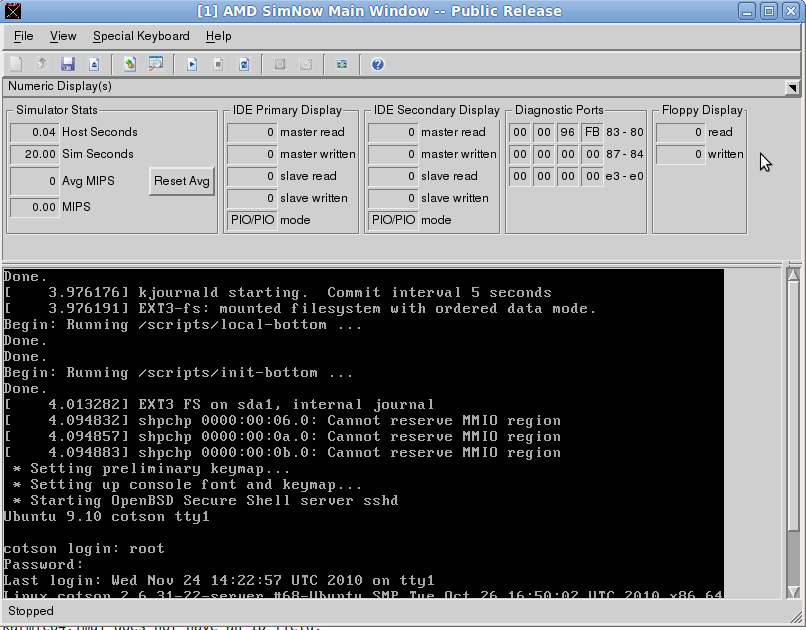
\includegraphics[width=3.0in,height=2.2in]{img1.png}
\par}

{\centering\selectlanguage{english}\sffamily\bfseries
\label{bkm:Ref388171082}Fig.
\stepcounter{Figure}{\theFigure} -- Graphical control window of the
COTSon simulator
\par}

{\selectlanguage{english}
At this point, you can click inside the
{\textquotedblleft}black{\textquotedblright} window (enlarge it to see
the last lines, the icon before the last one in the command bar), press
the {\textquotedblleft}play{\textquotedblright} button (seventh icon of
the command bar in this picture) and issue, e.g., an
{\textquoteleft}ls{\textquoteright} command. Once done, you can close
this window a return to the shell of the host system.}

\subsection[COTSon simulator: look at a glance]{COTSon simulator: look
at a glance}
{\selectlanguage{english}
COTSon is a simulation framework, whose aim is to provide an evaluation
platform for real systems like current multi-core Personal Computers
consisting of x86\_64 processors and all classical peripherals, and
running available operating systems such as Linux (or, not shown here,
Windows{\texttrademark}).}

{\selectlanguage{english}
It was originally developed by HP Labs and AMD, and it targets
cluster-level systems composed of hundreds or thousands of commodity
multi-core nodes and their associated devices connected through a
standard communication network like, e.g., a datacenter. }

{\selectlanguage{english}
An accurate evaluation may require to model not only the functional
behavior (like in common
{\textquotedblleft}virtualizers{\textquotedblright} like
VMWare{\texttrademark}, Virtualbox{\texttrademark} and similar) but
also the timing behavior of the architectural components. With COTSon
the evaluation can range from high-simulation speed (and an
{\textquotedblleft}idealistic timing model{\textquotedblright} of 1
instruction per cycle) through an accurate timing model (up to desired
level of accuracy). Moreover, COTSon can trade simulation speed with
accuracy by offering about seven built-in sampling policies that can
enhance greatly the simulation speed (and the user can provide his/her
own sampling policies).}

\subsection[Supported platforms]{Supported platforms}
{\selectlanguage{english}
In order to run COTSon the user needs a computer equipped with a 64 bit
processor. This is required in order to correctly run the AMD SimNow
\textsuperscript{(TM)} virtualization layer (this component is
available only for Linux AMD64 and Windows XP 64-bit version, however
the entire simulation framework is available only under the Linux
environment. Hereafter we refer to the virtualization layer simply as
SimNow). Currently, \textbf{COTSon} (\textbf{v680}) requires the
\textbf{4.6.2pub} version of SimNow, while it supports the following
Linux distributions:}

\begin{center}
\tablehead{}
\begin{supertabular}{|m{1.9316599in}|m{2.44206in}|m{1.6969599in}|}
\hline
\multicolumn{3}{|m{6.2281604in}|}{\centering
\selectlanguage{english}\bfseries Supported Linux
Distributions}\\\hline
\selectlanguage{english}\bfseries Debian &
\selectlanguage{english}\bfseries Fedora &
\selectlanguage{english}\bfseries Ubuntu\\\hline
\selectlanguage{english} Lenny &
\selectlanguage{english} Werewolf &
\selectlanguage{english} Intrepid\\\hline
\selectlanguage{english} Squeeze &
\selectlanguage{english} Leonidas &
\selectlanguage{english} Jaunty\\\hline
~
 &
\selectlanguage{english} Goddard &
\selectlanguage{english} Karmic\\\hline
~
 &
\selectlanguage{english} Laughlin &
\selectlanguage{english} Lucid\\\hline
~
 &
\selectlanguage{english} Lovelock &
\selectlanguage{english} Maverick\\\hline
~
 &
\selectlanguage{english} Verne &
\selectlanguage{english} Natty\\\hline
~
 &
\selectlanguage{english} Beefy Miracle &
\selectlanguage{english} Oneiric\\\hline
~
 &
\selectlanguage{english} Spherical Cow &
\selectlanguage{english} Precise\\\hline
~
 &
\selectlanguage{english} Schr\"odinger{\textquotesingle}s Cat &
\selectlanguage{english} Quantal\\\hline
~
 &
~
 &
\selectlanguage{english} Raring\\\hline
\end{supertabular}
\end{center}
{\centering\selectlanguage{english}\sffamily\bfseries
Table
\stepcounter{Table}{\theTable} -- COTSon installation: supported Linux
distributions.
\par}

{\selectlanguage{english}
The minimum hardware configuration required for the installation is as
follows: }

\begin{itemize}
\item {\selectlanguage{english}
\foreignlanguage{english}{\textit{Processor}}\foreignlanguage{english}{:
\ AMD
Athlon}\foreignlanguage{english}{\textsuperscript{(TM)}}\foreignlanguage{english}{
64 X2 Dual Core Processor 4600+ or equivalent; }}
\item {\selectlanguage{english}
\foreignlanguage{english}{\textit{Memory}}\foreignlanguage{english}{: 2
GB of main memory (8GB or more recommended);}}
\end{itemize}
{\selectlanguage{english}
Please also note that for licensing issues the simulator should be run
on AMD machines, even though Intel processors are also reported to
function).}


\bigskip

\subsubsection[Running COTSon in a virtualized environment]{\rmfamily
Running COTSon in a virtualized environment}
{\selectlanguage{english}
Installation under Windows environment is supported, through the use of
virtualization software (e.g., VirtualBox, VMware, etc.), by allocating
enough resources to the guest machine. This kind of installation is
also suited for shared environments, where a single server can host
several virtualized machines. In this case virtualized machine can be
remotely accessed. For further information on virtualization software,
please refer to the specific manual of AMD SimNow.}

\subsection[Document structure]{Document structure}
{\selectlanguage{english}
The rest of the document is organized as follows. Section 2 and section
3, are devoted to the description of the main characteristics of the
simulator. In particular, the guide focuses on the general
architecture, the mechanism implemented to collect timing information,
and the description of the main internal components (such as the
virtualization layer, the interleavers, the samplers, etc.). An entire
section is devoted to the user interface used to configure and interact
with the simulator. COTSon adopts the LUA language (see Appendix-1) to
provide a flexible way to describe the configuration of the target
system (i.e., the architecture of the system to be simulated), and the
parameters for the experiment setup (e.g., functional simulation vs.
timing simulation, structure for storing collected measures, commands
for the virtualization layer, etc.). Structures for collecting data
during simulation are deeply described in section 5, while section 6
presents to the user a set of simple examples that illustrate all the
features previously described. Following these examples the user should
be able to set-up the simulation environment, and to run architectural
simulations of interest. Finally, sections from 7 to 17 illustrate
advanced examples that reflect research activity carried out in the
TERAFLUX project at the scale of 1000+ cores [6][18]. They can be used
as a reference for setting-up advanced simulation experiments. In
particular, they can be used to understand how to extend the simulation
infrastructure.}

\section[Understanding COTSon: Design and Architecture]{Understanding
COTSon: Design and Architecture}
{\selectlanguage{english}
Simulation, combining some architectural structures, permits to create
virtual systems in which hardware components are shaped, in order to
make new functional units, or entire microprocessor systems. The aim of
a simulator is to show, record and analyze the performances and the
behavior of applications, and select the best architecture for each of
them. Simulators can be also used to develop new software and hardware
components that can be thus verified in their behavior. The increasing
complexity of computing systems has made simulators the first choice
for their design and analysis. In fact, a good simulator infrastructure
can help researchers, designers and developers in verifying if their
decisions are correct or not, possibly finding some optimal solutions.
Speed, accuracy, full-system capability and ability to extract specific
metrics are the main characteristics of a simulator and also what makes
one simulator different from another.}

{\selectlanguage{english}
{COTSon is a simulation framework targeting many-core
architectures, initially developed by HP Labs. The key feature of
COTSon is the adoption of a
}\textit{{functional-directed
}}{simulation }{approach, where fast
functional emulators and timing models cooperate to improve the
simulation accuracy at a speed sufficient to simulate the full stack of
applications, middleware and OS. }{Functional
simulation}\textit{{ }}{emulates the
behavior of the hardware components (e.g., common devices such as
disks, video, and network interfaces) of the target system, without
considering latency information. On the contrary,
}{timing simulation}\textit{{
}}{is used to assess the performance of the system. It
models the operation latency of devices simulated by the functional
simulator and assures that events generated by these devices are
simulated in a correct time ordering.}}

\subsection[Major Design Characteristics and comparison with other
simulators]{Major Design Characteristics and comparison with other
simulators}
{\selectlanguage{english}
Depending on how the functional and the timing parts of the simulator
are controlled and on their relationship, it is possible to define
different types of simulations:}

\begin{itemize}
\item {\selectlanguage{english}
\textit{Timing-directed or execution-driven}: here the timing model of
the simulator is in charge of driving the functional simulation. In
this case the functional and timing parts are programmed tightly
coupled to let the two parts cooperate easily;}
\item {\selectlanguage{english}
\textit{Functional-first or trace-driven}: in this case the functional
simulation produces an open-loop trace of the instructions that have
been executed. Then, these instructions will be passed to the timing
simulator. This type of simulator is usually built using particular
libraries such as Atom or Pin;}
\item {\selectlanguage{english}
\textit{Timing-first}: timing and functional models are decoupled and
timing drives the simulation. In this approach the timing simulator
precedes the functional simulator, and uses the latter to periodically
check and correct the simulation state (eventually functional execution
may have to be undone);}
\item {\selectlanguage{english}
\textit{Functional-directed}: timing and functional models are decoupled
and functional drives the simulation. In this approach was proposed to
treat better complex benchmarks and to afford greater speed
scalability; the timing feedback corrects the timing so that it becomes
visible to the application running on the simulated machine.}
\end{itemize}
{\selectlanguage{english}
COTSon uses the later approach (functional directed simulation: the
functional and timing simulation are clearly separated using two
interfaces. This approach allows reusing existing functional simulators
(very difficult to implement and maintain). COTSon{\textquotesingle}s
functional simulator is SimNow that functionally models most of the
existing hardware that can be found on a modern AMD system (in this
sense it supports generic X86\_64 architectures). SimNow contains also
the internal capability of timing simulation but such information is
completely discarded when used in conjunction with COTSon: only the CPU
capability is used in this case. COTSon is highly modular, and this
characteristic enables users to select different timing models,
depending on the particular experiment they want to perform. It is also
possible to program new timing models (e.g., a new coherence protocol)
or to adapt the existing ones (e.g., cache timing with MESI protocol),
and incorporate them into COTSon. Another very important aspect of
COTSon is the speed. In fact even if it is not significant in terms of
simulation results, a full system model simulator can be five or six
orders of magnitude slower than the real system, and this may become
unsustainable, as it limits the coverage of experiments. To speed up
the simulations COTSon uses virtual machine techniques for its
functional simulation (that comprehends just in time compiling and code
caching) and also sophisticated techniques such as
{\textquotedblleft}dynamic sampling{\textquotedblright}.}

\subsection[Timing Feedback]{Timing Feedback}
{\selectlanguage{english}
As discussed in the previous section, the aim of COTSon is to achieve
the best possible trade-off between simulation speed and accuracy for
many-cores systems (e.g., systems equipped with hundreds or even
thousands cores). To this end the design choice made was to use a
functional-directed approach, where the functional simulation of the
target architecture (fast) is periodically updated and its timing is
integrated with information coming from timing models of the
architecture components. }

{\selectlanguage{english}
In a pure trace-driven systems in fact, there is no influence on the
functional part coming from the timing part. This does not represent a
big limitation in case of single core systems, but can be a problem in
multicore systems. In fact the latter usually change their functional
behavior depending on their performance. For example, threads in a
multi-threaded application exhibit different interleaving patterns,
depending on the performance of each thread (possibly running on
different cores). On another level, many networking libraries such as
Message Passing Interface (MPI) change their policies and algorithms
depending on the particular performance of the network }

{\centering 
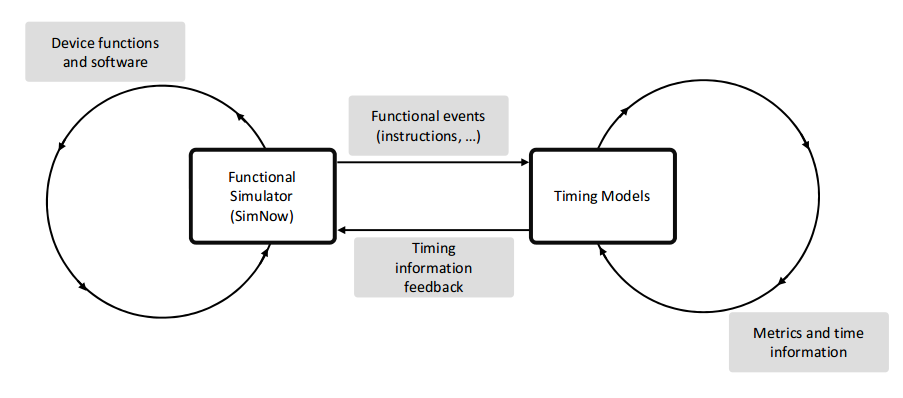
\includegraphics[width=4.6654in,height=2.0646in]{img2.png}
\par}

{\centering\selectlanguage{english}\sffamily\bfseries
Fig.
\stepcounter{Figure}{\theFigure} - Interaction between functional
simulation components and timing components in COTSon simulator.
\par}

{\selectlanguage{english}
Having \textit{timing feedback}, i.e., a communication path from the
timing to the functional simulator becomes fundamental for analyzing
this kind of situations. From this viewpoint, COTSon makes its
functional simulator run for a time interval ${\Delta}$t that is
dynamically set. The produced stream of references (i.e., instructions
and data memory accesses, but in general
{\textquotedblleft}events{\textquotedblright}) is sent to the
respective CPU timing models. At the end of such interval using the
metrics coming from the CPU models, the actual time interval to process
such stream of reference is known (say ${\Delta}$t{\textquoteright})
and it is given back to the functional simulator. The user can select
different interval sizes to choose the accuracy-speed trade-off.
Therefore, COTSon (realizing this trade-off between accuracy and speed)
enables users to avoid uninteresting parts of the code (such as initial
loading of the system) simulating them at lower accuracy.}

\subsection[Architecture]{Architecture}
{\selectlanguage{english}
The COTSon architecture has been developed having in mind the simulation
of clusters. From this viewpoint COTSon uses a SimNow instance to
represent each node of the cluster. SimNow has been augmented, by
HP-Labs and AMD, with a double communication layer to allow any device
to export functional events and obtain timing information. All the
events are directed by COTSon to the timing models. }

{\selectlanguage{english}
There are two types of communication mechanisms exhibited by devices:
synchronous and asynchronous. \textit{Synchronous }communication is
used for devices that immediately respond with timing information for
each event received (and the event does not occur very frequently). An
example of synchronous communication is the simulation of a disk read
by the functional simulator: a read event (instead of an interrupt) is
issued to COTSon, which delivers this event to a disk model that
determines the operation{\textquotesingle}s latency, which is used by
SimNow to schedule the functional interrupt, which signals the end of
the read. }

{\selectlanguage{english}
Synchronous communication is not usable when there is a high frequency
of events of this type (e.g., main memory accesses, CPU simulation,
etc.). In these cases \textit{asynchronous communication} is needed.
Differently from the synchronous case, the SimNow simulator does not do
a call per event, but produces
{\textquotedblleft}tokens{\textquotedblright} describing dynamic
events, that will be parsed by COTSon and delivered to the appropriate
timing modules. These modules will be asked by COTSon at specific
moments to aggregate timing information (in term of number of
instructions and cycles) and give them back to each functional core. }

{\centering 
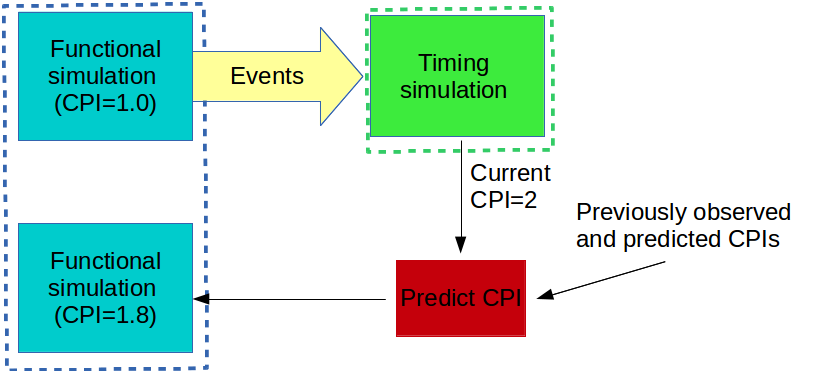
\includegraphics[width=3.8583in,height=1.7591in]{img3.png}
\par}

{\centering\selectlanguage{english}\sffamily\bfseries
\label{bkm:Ref388169507}Fig.
\stepcounter{Figure}{\theFigure} -- Example of timing feedback with
asynchronous communication for estimating the IPC in COTSon.
\par}

{\selectlanguage{english}
For example, in Fig. 3 we show the situation when a timing module is
used for a processor pipeline with the purpose of estimating the number
of Cycles Per Instruction (CPI). The resulting CPI, given back to the
functional module, is used by SimNow to schedule the progress of
instructions in each core and in this way the timing feedback is used
for the functional simulations. However in many situations the timing
feedback has to be filtered and modified, in order to obtain an
increase in simulation accuracy. For example if a particular core is
mostly idle it doesn{\textquotesingle}t give an accurate estimate of
the CPI. To solve this problem, COTSon offers a timing feedback
interface that handles these modifications transparently. This
interface is able to correct and predict future CPI by using
mathematical models, such as Auto-Regressive-Moving-Average (ARMA)
model, that is used, e.g., in forecasting time series. A simple example
of the timing feedback mechanism is shown in Fig. 3.}

\subsection[COTSon installation structure]{COTSon
\foreignlanguage{english}{installation} structure}
{\selectlanguage{english}
Once COTSon is installed the user will get a directory structure as
follows:}

\begin{itemize}
\item {\selectlanguage{english}
\textit{bin}: contains binaries of the simulator;}
\item {\selectlanguage{english}
\textit{data}: contains the \textit{bsd} images and the \textit{disk}
images used to run simulations;}
\item {\selectlanguage{english}
\textit{share contains some common scripting files};}
\item {\selectlanguage{english}
\textit{src}: contains all the files related to the development of the
simulator;}
\item {\selectlanguage{english}
\textit{sandbox}: it{\textquoteright}s the template of a
{\textquoteleft}sandbox{\textquoteright} on the host used to control a
node during the simulation}
\item {\selectlanguage{english}
\textit{etc}: COTSon general configuration files}
\item {\selectlanguage{english}
\textit{sbin}: COTSon general system binaries}
\item {\selectlanguage{english}
\textit{daemon}: contains files for running the simulator in a
distributed environment (not described in this document);}
\item {\selectlanguage{english}
\textit{web}: COTSon web control (not described in this document)}
\end{itemize}
{\selectlanguage{english}
The \textit{src} directory has the following structure:}

\begin{itemize}
\item {\selectlanguage{english}
\textit{src/abaeterno}\textbf{\textit{/}} it is the core COTSon
infrastructure. This directory contains timers, samplers and the simnow
interface; }
\item {\selectlanguage{english}
\textit{src/common/} common utilities (metrics, options, etc.) for
abaeterno and network;}
\item {\selectlanguage{english}
\textit{src/disksim/} disksim distribution for COTSon;}
\item {\selectlanguage{english}
\textit{src/distorm/} distorm (x86 disassembler) for COTSon;}
\item {\selectlanguage{english}
\textit{src/examples/} simple simulation examples (we will analyze them
after );}
\item {\selectlanguage{english}
\textit{src/libluabind/} C++ binding for LUA (used for COTSon
scripting);}
\item {\selectlanguage{english}
\textit{src/network/} COTSon (HP) network mediator (for distributed
synchronization);}
\item {\selectlanguage{english}\itshape
src/mcpat \ used for power and area estimation through the \ HP McPAT
tool}
\item {\selectlanguage{english}
\textit{src/slirp/} slirp library (NAT access from guest) for COTSon;}
\item {\selectlanguage{english}
\textit{src/test.regression/} simple regression tests;}
\item {\selectlanguage{english}
\textit{src/tools/} tools to support simulation experiments;}
\end{itemize}

\bigskip

\section[COTSon components: SimNOW, Samplers, Interleaver,
Timers]{COTSon components: SimNOW, Samplers, Interleaver, Timers}
{\selectlanguage{english}
The main parts of a COTSon node, are the functional simulator SimNow,
the timing models (timers), the sampler, the interleaver, and the time
predictor. Moreover, the network \textit{Mediator} and the
\textit{Control} are two components of COTSon that allow the simulation
of cluster configurations (Fig. 4). The dynamically loaded library
(DLL) \textit{abaeterno}, is also a fundamental part of COTSon,
because, when loaded by SimNow, it determines the time the simulation
is taking, and it contains the implementation of all types of timers,
samplers, etc., that can be used by COTSon.}

{\centering 
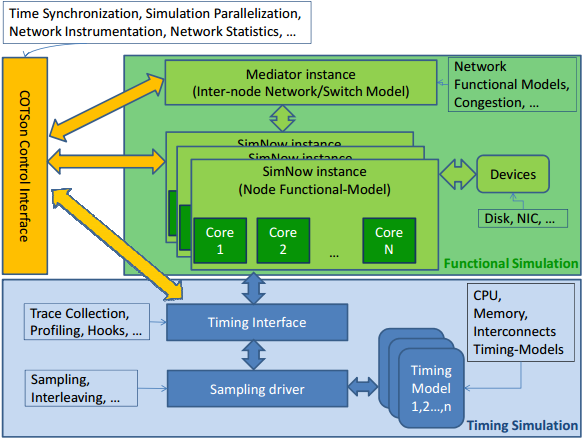
\includegraphics[width=5.7965in,height=4.3591in]{img4.png}
\par}

{\centering\selectlanguage{english}\sffamily\bfseries
\label{bkm:Ref388170339}Fig.
\stepcounter{Figure}{\theFigure} -- COTSon components overview
\par}

\subsection[Virtualizer: short introduction to SimNow]{Virtualizer:
short introduction to SimNow}
{\selectlanguage{english}
It implements the x86 and x86\_64 instruction sets, including system
devices. It allows the user to configure a full-system architecture by
changing the various components (i.e., CPU type, number of CPUs,
organization, main memory size, etc.). }

{\selectlanguage{english}
SimNow provides several CPU models, dynamic translation of instructions
(the instruction input stream is translated into C-like language and
then is compiled for the native machine) and deterministic execution;
it can simulate the majority of existing hardware uniprocessor and
multiprocessor that are available on a modern AMD system. It also uses
caching techniques and supports the booting of an unmodified Operating
System (such as Windows and Linux) over which some complex applications
can be executed. In full-speed mode SimNow performance is around
100-200 MIPS (i.e., it has a 10x slowdown with respect to the native
execution). It comes with several Broad-Sword Document (BSD)
configurations, i.e., files containing setup parameters of a simulated
target machine. The host machine, in which the simulator runs, and the
guest machine, i.e. the simulated machine, can communicate through a
toolbox called \textit{Xtools}, mainly constituted of two commands: i)
xput, which is run on the guest to copy a file from the guest to the
host and ii) xget, which is run in th guest to copy a file from the
host to the guest SimNow can be controlled from the shell (command line
mode) or through a User Interface Window (graphical mode -- see Fig.
5). When using the graphical mode, users see and modify the target
system configuration (i.e., the configuration of simulated devices such
as disk images, BIOS, DRAM and CPU) from the main windows, and they can
access to the results of the simulation as well. The main window is
divided in two main parts: one shows time results of the simulation,
while in the other a console provides a textual interface for status
information and a command-line control for the guest OS running in the
host.}

{\selectlanguage{english}
The part showing time results is called SimStats and it is composed of 4
components:}

\begin{itemize}
\item {\selectlanguage{english}
\textit{Host Seconds} (1): showing the number of seconds spent (both in
user and system mode) by the host CPU, since the simulation has
started;}
\item {\selectlanguage{english}
\textit{Sim Seconds} (2): showing the time spent in the simulation since
it has started;}
\item {\selectlanguage{english}
\textit{Avg MIPS} (3): showing the instantaneous values of the simulator
performances, that is measured in millions of executed (simulated)
instructions per host.}
\end{itemize}
\begin{itemize}
\item {\selectlanguage{english}
\textit{MIPS} (4): showing the number of simulated instructions from the
start of the simulation, divided by host seconds;}
\end{itemize}

\bigskip

{\selectlanguage{english}
Below there is the \textit{Console Window} (5): providing the guest
output and control for the guest OS;}

{\centering 
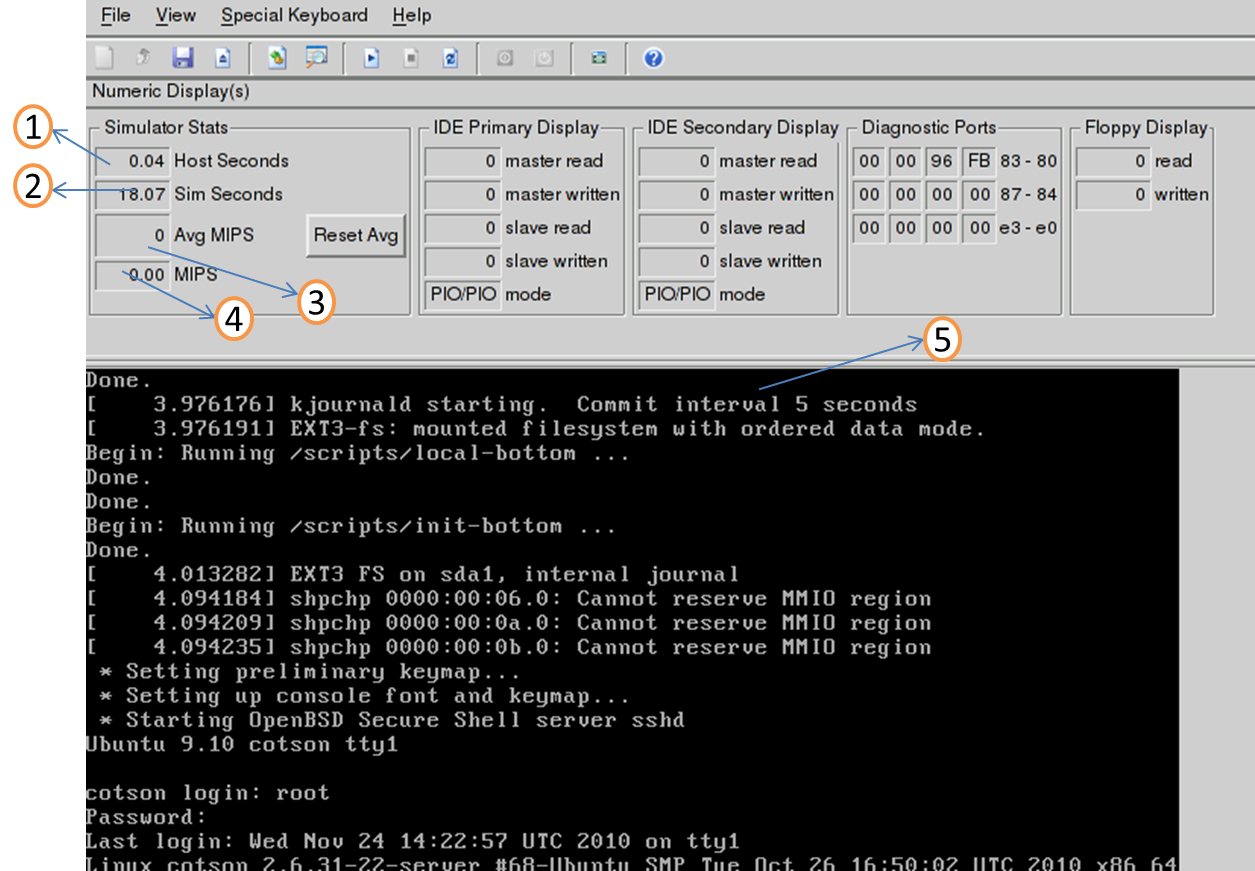
\includegraphics[width=5.2453in,height=3.652in]{img5.png}
\par}

{\centering\selectlanguage{english}\sffamily\bfseries
\label{bkm:Ref388170369}Fig.
\stepcounter{Figure}{\theFigure} -- Graphical interface of the COTSon
simulator. The window contains a toolbar from which interact with the
simulator, a panel displaying statistical information, and a control
panel from which interact with the guest system.
\par}

\subsection[Samplers]{Samplers}
{\selectlanguage{english}
COTSon can be configured to use a full-speed functional modality or a
sampled modality. The samplers are one of the most important parts of
COTSon infrastructure, as they represent the way functional and timing
simulations are integrated together. This can be seen also in Fig. 4,
where the sampler is placed between the front-end (functional
simulator) and the back-end (timing models of the architectural
components) of the COTSon node. Sampling is crucial for asynchronous
devices and it is the process through which the timing simulation (or
simply simulation) is turned off or on. A good sampler is required to
select a simulation interval such that the simulation metrics taken in
that interval well approximates the statistics of the whole execution.
So the timing simulation will be performed only in appropriate moments
and for an appropriate duration, thus avoiding the slow-down of timing
simulation.}

{\selectlanguage{english}
The type of sampler required for a certain experiment and the lengths
and the type of the samples can be configured by writing proper values
in the COTSon configuration file (see Section 4). With this
information, the sampler gives a command to enter one of the following
phases:}

\begin{itemize}
\item {\selectlanguage{english}
\textit{Functional}: during this phase only functional simulation is
performed and so no events are produced by the simulated devices, that
so are simulated at full speed;}
\item {\selectlanguage{english}
\textit{Warming} (simple/detailed): this phase is necessary to pass from
functional to timing simulation; during it the timing models are warmed
up to prepare them to the timing simulation. If only the
high-hysteresis elements (such as caches and branch target buffers) are
warmed up, the warming is said to be simple, otherwise, if also the
low-hysteresis elements (such as reorder buffers and renaming tables)
are warmed up, the warming is called detailed;}
\item {\selectlanguage{english}
\textit{Simulation}: this phase is the opposite of the functional phase.
Here the devices must produce events that are sent to the timing
models, so that timing simulation can be performed;}
\end{itemize}
{\selectlanguage{english}
In order to determine sampling intervals, it is necessary to find out
what are the most representative and relevant parts of the
application{\textquotesingle}s execution. This selection is based on
the phase analysis, which determines the phases of a program, i.e., the
parts of the execution that have a similar behavior, independently of
temporal adjacency. Depending on how the phases of a program are
detected different samplers can be implemented. The most important
samplers are \textit{SMARTS}, \textit{SimPoint}, \textit{dynamic
}samplers, and \textit{interval-based} samplers. The first two require
an a priori profiling or a preprocessing of the code and
don{\textquotesingle}t allow timing feedback. }

{\centering 
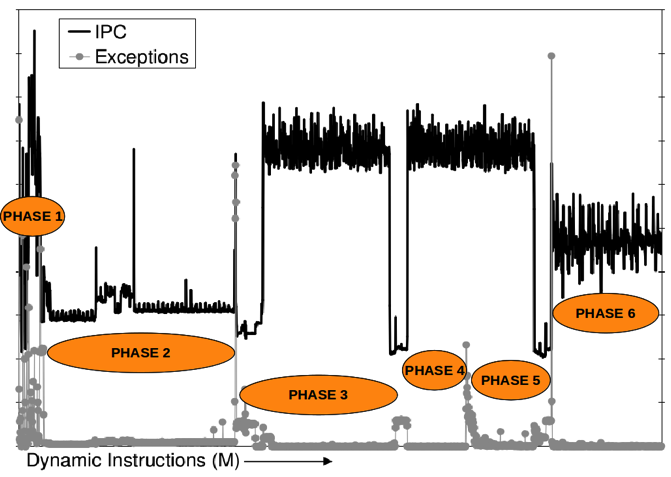
\includegraphics[width=3.0465in,height=2.1654in]{img6.png}
\par}

{\centering\selectlanguage{english}\sffamily\bfseries
\label{bkm:Ref388170448}Fig.
\stepcounter{Figure}{\theFigure} -- Correlation of the performance
information acquired by the simulator with the running application
phases.
\par}

{\selectlanguage{english}
Because of these two characteristics, they result to be less flexible
than dynamic samplers and may be subject to errors due to the absence
of timing feedback. In the interval-based sampler the duration of each
phase (state) of the sampling (functional, warming, simulation) is
fixed. Dynamic Sampling is based on the consideration that all
functional simulators (such as fast emulators, like SimNow, or virtual
machines, like VMware) keep track of internal statistics of two types:}

\begin{itemize}
\item {\selectlanguage{english}
Those related to their internal structures (translation cache, software
TLB), such as code cache invalidations, code exceptions, and I/O
operations;}
\item {\selectlanguage{english}
Those related to the emulated code, such as number of executed
instructions, memory accesses, exceptions, and bytes read or written to
or from a device;}
\end{itemize}
{\selectlanguage{english}
Both types of metrics are strictly related to the behavior and the
performance of the emulated software and can be used to detect phase
changes in an application{\textquotesingle}s execution. Fig. 6 shows an
example of how an internal statistic (number of code Exceptions) is
correlated to the application{\textquotesingle}s performance (IPC) and
thus to the application{\textquotesingle}s phases. The dynamic sampler
lets a timing simulation start whenever the first-derivative of the
chosen internal statistic overcomes a threshold. After a certain number
of instructions, the simulation returns to be functional, until the
next phase change is detected, and so on. Fig. 7 shows a schematic view
of how Dynamic Sampling works.}

{\centering 
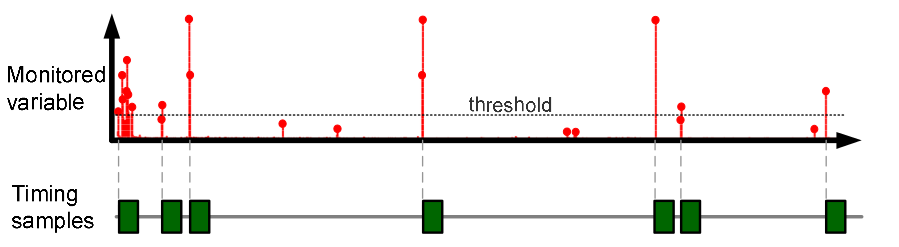
\includegraphics[width=5.3752in,height=1.4819in]{img7.png}
\par}

{\centering\selectlanguage{english}\sffamily\bfseries
\label{bkm:Ref388170462}Fig.
\stepcounter{Figure}{\theFigure} - A schematic representation of how
dynamic sampling works.
\par}

{\selectlanguage{english}
Different types of samplers can be selected by the user, writing
appropriate values in the COTSon (LUA) configuration file. }

\subsection[Interleavers]{Interleavers}
{\selectlanguage{english}
The interleaver is a component that is used during the simulation of SMP
(Symmetric Multi-Processor), i.e., multi-core systems. In fact, it
supervises the buffering and the reordering of the events coming from
the functional simulation. These operations are fundamental when
multiple cores are simulated. To this end, SimNow simulates multi-cores
with an interleaved sequence. After a certain interval of time, called
\textit{synchronization quantum}, during which the cores operate
independently, all the cores arrive to the same point in time. After
the synchronization quantum, all the events are stored in a queue and
then they are interleaved. Only at this moment they are ready to be
carried to the timing models of the CPUs.}

\subsection[Timers]{Timers}
{\selectlanguage{english}
There is a timer for each architectural component that can be simulated,
and its role is to collect events coming from the functional
simulation, and use them to update the timing model of the component.
In other words a timer is software that simulates the timing behavior
of each component. There are timers for the CPU, for the Memory, for
the disks, and for the NIC (Network Interface). The type of timer
(e.g., timer0 -- for an in-order superscalar processor, timer1 -- for
an out-of-order superscalar processor, bandwidth -- for measuring the
memory bandwidth, etc.) can be set in the COTSon configuration file.
The feedback information is governed by the \textit{time predictor}:
based on the metrics collected by the timing simulation, it decides how
to feedback information to the functional simulator.}

\section[COTSon configuration]{COTSon configuration}
{\selectlanguage{english}
A simple COTSon configuration file (written in lua file
{\textquoteleft}functional.in{\textquoteright}) to run a functional
simulation is shown in Fig. 8. It uses the {\textquoteleft}functional
template (first line), shows a graphical display for Simnow (second
line), where ({\textquoteleft}simnow.commands{\textquoteright}) the
architectural configuration of the SimNow uses the
{\textquoteleft}1p.bsd{\textquoteright} (fourth line, that also stores
the snapshots and modifications of the running simulation), an
off-the-shelf hard disk image with the Operating System (this remains
unmodified during the simulation, fifth line), and we enable the
journaling of the file system (sixth line)}

{\centering 
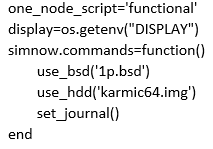
\includegraphics[width=2.2189in,height=1.552in]{img8.png}
\par}

{\centering\selectlanguage{english}\sffamily\bfseries
\label{bkm:Ref388172416}Fig.
\stepcounter{Figure}{\theFigure} -- A simple COTSon configuration file
(written in lua file {\textquoteleft}functional.in{\textquoteright}
\par}

\subsection[Lua Scripting]{\selectlanguage{english} Lua Scripting}
{\selectlanguage{english}
The COTSon simulation infrastructure is controlled by setting all the
relevant information about simulation and the target system
configuration in an input configuration file. COTSon uses \textit{Lua
scripting language} to manage this configuration file. The Lua
scripting language is powerful, fast, lightweight, and embeddable. It
combines simple procedural syntax with powerful data description
constructs based on associative arrays and extensible semantics. Lua is
dynamically typed, runs by interpreting bytecode for a register-based
virtual machine, and has automatic memory management with incremental
garbage collection, making it ideal for configuration, scripting, and
rapid prototyping. For further information about Lua language syntax,
see Appendix A -- Lua lexical conventions, and Appendix B -- Lua
language features.}

{\selectlanguage{english}
Suppose the user wants to run the functional example
(\textit{functional.in}) present in the directory
\texttt{cotson/src/examples}:}

\begin{flushleft}
\tablehead{}
\begin{supertabular}{|m{6.29346in}|}
\hline
\selectlanguage{english} \texttt{\$ cd cotson/src/examples}\\\hline
\end{supertabular}
\end{flushleft}
{\selectlanguage{english}
Then simply issue the command:}

\begin{flushleft}
\tablehead{}
\begin{supertabular}{|m{6.29346in}|}
\hline
\selectlanguage{english} \texttt{\$ ../../bin/cotson
functional.in}\\\hline
\end{supertabular}
\end{flushleft}
{\selectlanguage{english}
This will launch the SimNow window as explained in Section 1.2 (Step 2:
running a first example).}

{\selectlanguage{english}
One of the nice features of the Lua scripts is that they accept Lua
parameters either in files or in the command line. Anything that is not
strictly an existing object, is considered part of the Lua syntax (see
Appendix A -- Lua lexical conventions). The Lua script is the
concatenation of the contents of all the files and the Lua syntax, and
it is passed to any part of COTSon that would need it (like the COTSon
Control script -- named {\textquoteleft}cotson{\textquoteright}, the
{\textquoteleft}abaeterno{\textquoteright} library). Even if not every
part of the elements written in the Lua file is needed by these
components, each of them can select the parts that are needed.}

\subsection[Changing the configuration]{Changing the
\foreignlanguage{english}{configuration}}
{\selectlanguage{english}
The Lua configuration file used in COTSon is divided into 3 main
sections:}

\begin{itemize}
\item {\selectlanguage{english}
\textit{LUA-SECTION-1}: describes general simulation options. This part
is called \textit{options table;}}
\item {\selectlanguage{english}
\textit{LUA-SECTION-2}: describes options/commands for SimNow. This part
is called \textit{SimNow table}, and is used by the control scripts to
determine how to set up the SimNow execution;}
\item {\selectlanguage{english}
\textit{LUA-SECTION-3}: describes the target system configuration in
details. This part is called \textit{build function. }Anything inside
it or in the \textit{options table} is used by the abaeterno library.
(Anything that follows may be by the COTSon control and web interface
to determine what kind of execution to make);}
\end{itemize}
\subsubsection[Lua{}-Section{}-1 {}--options
table]{\foreignlanguage{english}{\textrm{Lua-}}\textrm{S}\foreignlanguage{english}{\textrm{ection-}}\textrm{1}\foreignlanguage{english}{\textrm{
}}\foreignlanguage{english}{\textrm{{}--}}\foreignlanguage{english}{\textrm{o}}\textrm{ptions}\foreignlanguage{english}{\textrm{
table}}}
{\selectlanguage{english}
This first section in the Lua file is delimited by:}

\begin{flushleft}
\tablehead{}
\begin{supertabular}{|m{6.29346in}|}
\hline
\selectlanguage{english}\ttfamily options=\{\}\\\hline
\end{supertabular}
\end{flushleft}

\bigskip

{\selectlanguage{english}
Here several options can be specified, in particular, the following
variables can be set:}

\begin{itemize}
\item {\selectlanguage{english}
\textit{max\_nanos}: is the variable where we specify how long we want
the simulation to last in terms of nanoseconds (e.g.
{\textquotedblleft}10M{\textquotedblright}, see Fig. 9);}
\item {\selectlanguage{english}
\textit{sampler}: where the type and the various options of the sampler
chosen can be specified (e.g.
type={\textquotedblright}simple{\textquotedblright} indicates a
detailed timing simulation (the opposite of the pure functional
simulation) and quantum={\textquotedblright}100k{\textquotedblright}
indicates how often the functional part has to synchronize with the
timing part -- see Fig. 9); also note how we can nest multiple lua
commands.}
\item {\selectlanguage{english}
\textit{heartbeat: }this is used to specify how to log statistics (e.g.,
type={\textquotedblright}file\_last{\textquotedblright} indicates to
dump all statistics in a file at the end of the simulation and in such
case
logfile={\textquotedblright}on\_cpu\_simple.log{\textquotedblright}
indicates the name of the file -- see Fig. 9). There can be
instantiated up to eight heartbeat options
({\textquotedblleft}heartbeat={\textquotedblright},
{\textquotedblleft}heartbeat1={\textquotedblright},
{\dots},{\textquotedblright} heartbeat7={\textquotedblright}).}
\end{itemize}

\bigskip

{\selectlanguage{english}
Other general options can be:}

\begin{itemize}
\item {\selectlanguage{english}
\textit{max\_samples}: here the maximum number of samples is specified;}
\item {\selectlanguage{english}
\textit{fastforward}: here it can be specified an amount of time that
will be skipped by the simulation;}
\end{itemize}
{\selectlanguage{english}
There are also several other types of sampler available like dynamic,
interval (see Section 6.3 {\textquotedblleft}Samplers: timing
simulation{\textquotedblright}). Similarly for the \textit{heartbeat,
}it is possible to use the sqlite database (or files) and the
statistics can be dumped at intervals during the simulation -- see
Section 5.2 Database structure for more details). Whenever the results
are stored in the database, the user has to specify also two particular
fields that are \textit{experiment\_id} and \textit{experiment\_
description}, needed to store the data in the correct field inside the
database tables for storing more experiments. Below (Fig. 9) an example
of COTSon configuration file -- section 1, taken from the file
\textit{one\_cpu\_simple.in} is shown.}

{\centering 
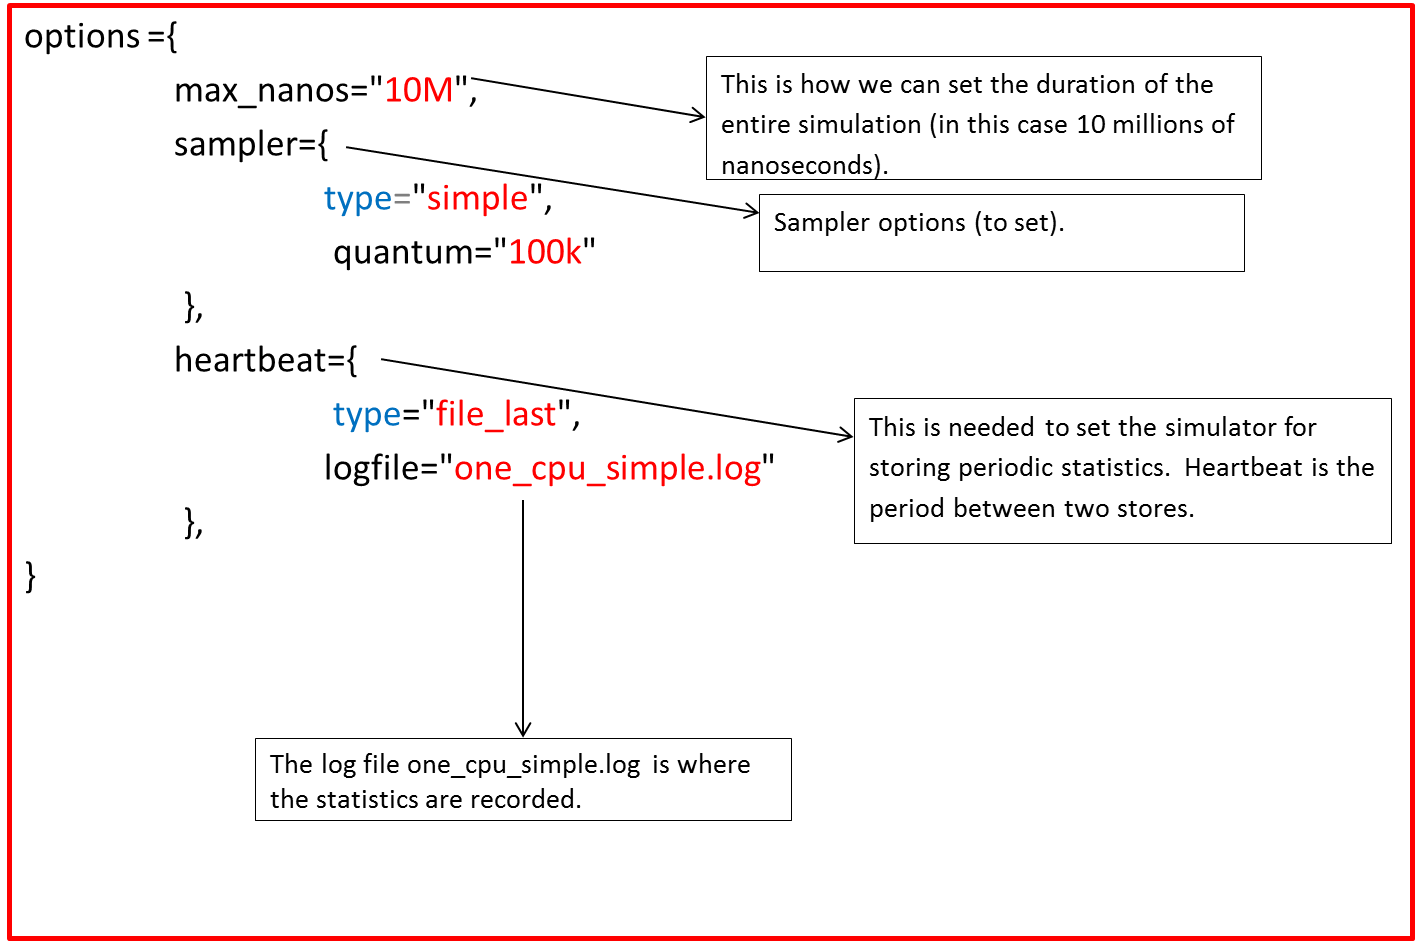
\includegraphics[width=5.2252in,height=3.4811in]{img9.png}
\par}

{\centering\selectlanguage{english}\sffamily\bfseries
\label{bkm:Ref388170511}Fig.
\stepcounter{Figure}{\theFigure} - An example of lua-section-1 of the
COTSon configuration file (see also the example
src/example/one\_simple\_cpu.in).
\par}

\subsubsection[Lua{}-Section{}-2 {}-- SimNow
options/commands]{\foreignlanguage{english}{\textrm{Lua-}}\textrm{S}\foreignlanguage{english}{\textrm{ection-}}\textrm{2}\foreignlanguage{english}{\textrm{
}}\foreignlanguage{english}{\textrm{{}--
}}\foreignlanguage{english}{\textrm{SimNow options/commands}}}
{\selectlanguage{english}
This section is opened by the line:}

\begin{flushleft}
\tablehead{}
\begin{supertabular}{|m{6.29346in}|}
\hline
\selectlanguage{english}\ttfamily simnow.commands=function()\\\hline
\end{supertabular}
\end{flushleft}
{\selectlanguage{english}
This part is where the SimNow commands are grouped. Then the following
options must be set (depending on the type of example the user is
running, it can use a subset of the options listed below):}

\begin{itemize}
\item {\selectlanguage{english}
\textit{use\_bsd( )}: here the bsd location is set. Possible types of
bsd are available in the folder cotson/data.}
\item {\selectlanguage{english}
\textit{use\_hdd( )}: here we set the position of where the hard disk
image is located, for example karmic64.img is available in the folder
cotson/data.}
\item {\selectlanguage{english}
\textit{set\_journal( )}: this function is needed to enable the
journaling of the file system.}
\item {\selectlanguage{english}
\textit{send\_keyboard( )}: this function allows the user to run a
command inside the OS of the simulated machine.}
\end{itemize}
{\selectlanguage{english}
In Fig. 10 the reader can see an example of lua-section-2, taken from
\textit{one\_cpu\_simple.in}. Other option (not show in Fig. 10 - An
example of lua-section-2 of the COTSon configuration file (see also
one\_simple\_cpu.in)) can be:}

\begin{itemize}
\item {\selectlanguage{english}
\textit{execute( )}: here the user can select the name of a (guest) file
to be executed during the simulation (e.g., a bash script file). This
file is copied from the host to the guest at the beginning of the
simulation and has to be in the same folder where the lua script is
stored.}
\item {\selectlanguage{english}
\textit{subscribe\_result( )}: serves to automatically copy the listed
files from the guest to the host at the end of the simulation.}
\end{itemize}
{\centering\selectlanguage{english}
\ \ 
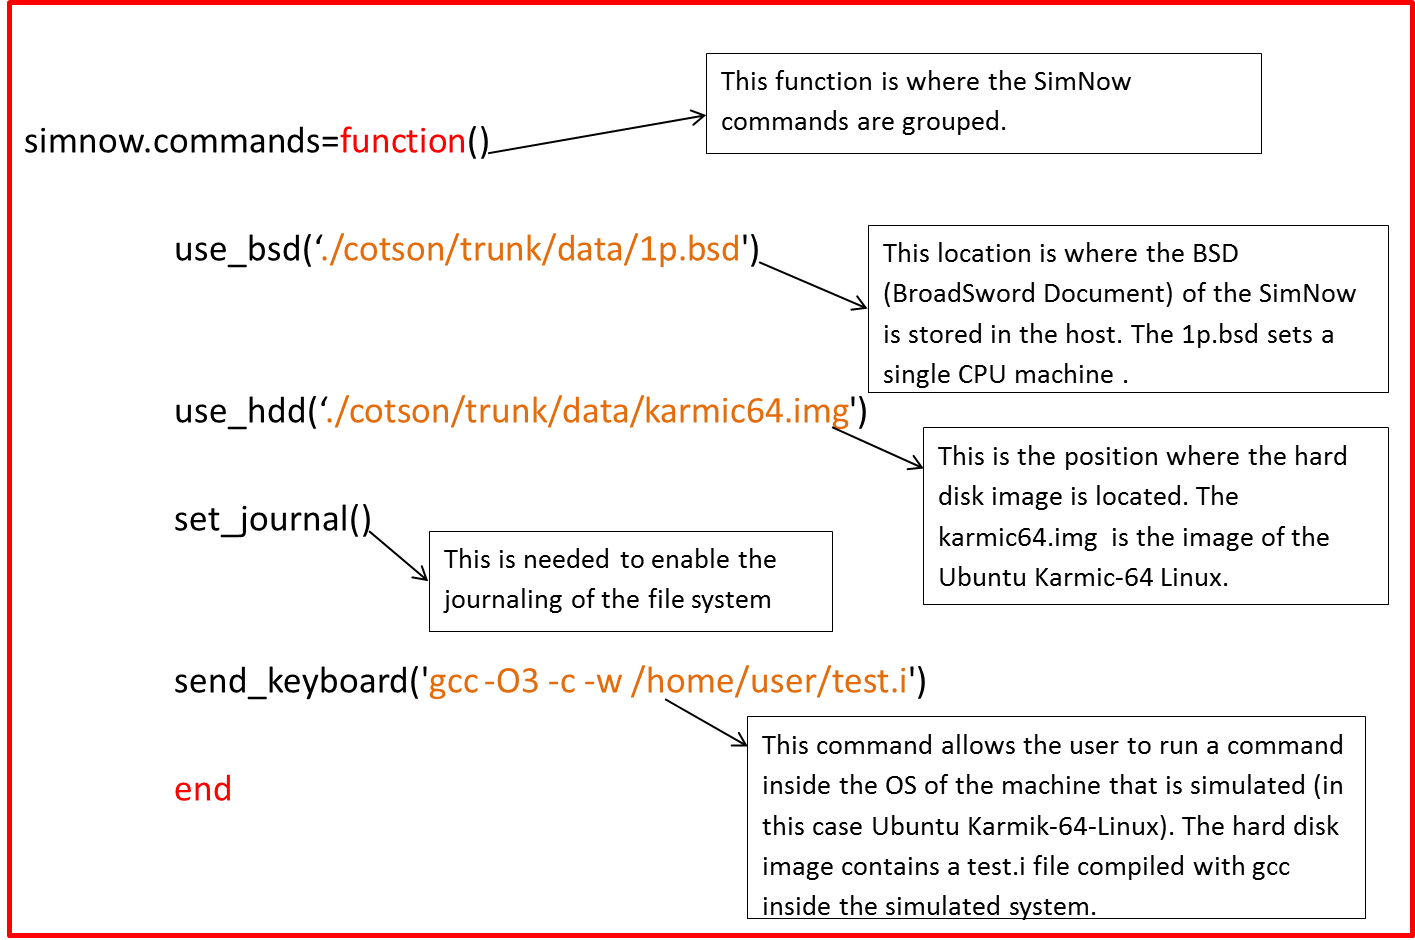
\includegraphics[width=4.4709in,height=2.9756in]{img10.png}

\par}

{\centering\selectlanguage{english}\sffamily\bfseries
\label{bkm:Ref388176688}\label{bkm:Ref388170520}Fig.
\stepcounter{Figure}{\theFigure} - An example of lua-section-2 of the
COTSon configuration file (see also one\_simple\_cpu.in)
\par}

\subsubsection[Lua{}-Section{}-3 {}-- configuration
options]{\foreignlanguage{english}{\textrm{Lua-}}\textrm{S}\foreignlanguage{english}{\textrm{ection-}}\foreignlanguage{english}{\textrm{3
}}\foreignlanguage{english}{\textrm{{}--
}}\foreignlanguage{english}{\textrm{configuration o}}\textrm{ptions}}
{\selectlanguage{english}
This section begins with the command (see Fig. 11):}

\begin{flushleft}
\tablehead{}
\begin{supertabular}{|m{6.29346in}|}
\hline
\selectlanguage{english}\ttfamily function build()\\\hline
\end{supertabular}
\end{flushleft}
{\selectlanguage{english}
After that, there is a part where the number of disks in the system is
specified and for each disk the appropriate timer is set. Then, in the
same way, it is found the number of the various Network Interfaces
attached to the system and to each one a timer is assigned. Then we can
specify the number of CPUs that are in the system. If the number is
zero, the simulation is stopped. The numbering of the disks, NICs, CPUs
will begin from zero (i.e., in a multi-core system CPUs are named as
cpu0, cpu1, etc.). Similarly to disks and NICs, to each CPU a
particular timer is assigned (e.g.
{\textquotedblleft}timer0{\textquotedblright} means a simple
superscalar in-order processor). For the memory and caches, it is
possible to decide the values of their main features, such as the
latency. The memory is set following a hierarchical approach, in other
words, usually the setting starts from the main memory, then the cache
with its levels. For each cache level, we can set the values of some
important variables, such as:}

\begin{itemize}
\item {\selectlanguage{english}
\textit{name}: determines the name of the considered cache level;}
\item {\selectlanguage{english}
\textit{size}: determines the total size of the considered cache level;}
\item {\selectlanguage{english}
\textit{latency}: determines the hit latency to access the considered
cache level;}
\item {\selectlanguage{english}
\textit{num\_sets}: determines the number of sets that are present in
the considered cache level;}
\end{itemize}
\begin{itemize}
\item {\selectlanguage{english}
\textit{write\_policy}: determines the write policy of the considered
cache level ({\textquotedblleft}WB{\textquotedblright} means Write
Back, {\textquotedblleft}WT{\textquotedblright} means Write Through);}
\item {\selectlanguage{english}
\textit{write\_allocate}: if it is set to true, it means that the
considered cache level is of type {\textquotedblleft}write
allocate{\textquotedblright}, otherwise, the cache is of type
{\textquotedblleft}write-no-allocate{\textquotedblright};}
\end{itemize}

\bigskip

{\selectlanguage{english}
Once all the memory components are set, we can connect them to the CPU
using some particular commands such as:}

\begin{flushleft}
\tablehead{}
\begin{supertabular}{|m{6.29346in}|}
\hline
{\selectlanguage{english}\ttfamily cpu:instruction\_cache(ic)}

{\selectlanguage{english}\ttfamily cpu:data\_cache(dc)}

{\selectlanguage{english}\ttfamily cpu:instruction\_tlb(it)}

\selectlanguage{english}\ttfamily cpu:data\_tlb(dt).\\\hline
\end{supertabular}
\end{flushleft}
{\selectlanguage{english}
All the various parts previously described, can be seen in Fig. 11,
which is an example of lua-sections3, again taken from
\textit{one\_cpu\_simple.in}.}

{\centering
% Unhandled or unsupported graphics:
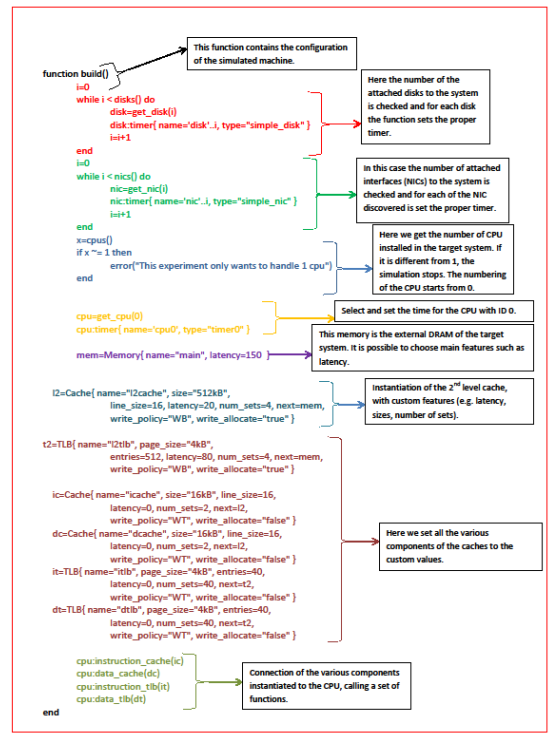
\includegraphics[width=5.7807in,height=7.7654in]{img11.png}
 \par}

{\centering\selectlanguage{english}\sffamily\bfseries
\label{bkm:Ref388170491}Fig.
\stepcounter{Figure}{\theFigure} - An example of lua-section-3 of the
COTSon configuration file (see also the example
src/example/one\_simple\_cpu.in)
\par}

\section[Collecting Metrics]{Collecting Metrics}
{\selectlanguage{english}
All the collected simulation measures can be permanently stored in a
specific data structure. The user can chose which structure to use for
storing information. The simulator provides two types of storing
structures: the simplest is a \textit{log file}, while the more
advanced is represented by a \textit{database}. Log file is generally
enough to store data collected during a simulation. However, for
keeping track of measures collected over several simulations, the
database is the best choice. It allows maintaining information
structured and it allows easily finding specific data by simply
querying it. COTSon uses a flexible data storage resorting to a SQL
server. By doing so, COTSon allows to search through simulation results
in a more consistent way using a familiar declarative language like
SQL.}

\subsection[Log structure]{Log structure}
{\selectlanguage{english}
A \textit{log file} is a simple text file, where all the information
gathered by the simulator during a simulation is written. Since it is a
text file, it can be automatically parsed at the end of the simulation.
The main drawback of this structure is that it grows rapidly with the
increase of simulation complexity. }

\subsection[Database structure]{Database structure}
\label{bkm:Ref388175692}\label{bkm:Ref388175687}{\selectlanguage{english}
The simplest way to use a SQL server to store simulation heartbeats
(i.e., periodic information collected by the simulator, such as
instruction count, memory read misses, etc.) is to use SQLite server
(currently at version 3). It should be installed by default with the
Linux distribution. However, it is possible to check for its presence
by using the following command:}

\begin{flushleft}
\tablehead{}
\begin{supertabular}{|m{6.29346in}|}
\hline
\selectlanguage{english} \foreignlanguage{english}{\texttt{\$
sqlite3}}\\\hline
\end{supertabular}
\end{flushleft}

%\bigskip

\begin{flushleft}
\tablehead{}
\begin{supertabular}{|m{6.29346in}|}
\hline
\selectlanguage{english} \foreignlanguage{english}{\texttt{\$ cd
src/examples; make run\_sqlite}}\\\hline
\end{supertabular}
\end{flushleft}
{\selectlanguage{english}
\foreignlanguage{english}{One example that uses the database is governed
by the {\textquotedblleft}sqlite.in{\textquotedblright} lua script in
the
}\foreignlanguage{english}{\texttt{src/examples}}\foreignlanguage{english}{
directory. To run it:}}

{\selectlanguage{english}
You can check the content of the database by issuing:}

\begin{flushleft}
\tablehead{}
\begin{supertabular}{|m{6.29346in}|}
\hline
\selectlanguage{english}\ttfamily \$ sqlite3 /tmp/test.db\\\hline
\end{supertabular}
\end{flushleft}
{\selectlanguage{english}
\foreignlanguage{english}{The tables in the database (hereafter DB for
simplicity) can be analyzed by typing the following command (the
}SQLite\foreignlanguage{english}{ server prompt is presented to the
user):}}

\begin{flushleft}
\tablehead{}
\begin{supertabular}{|m{6.29346in}|}
\hline
\selectlanguage{english}\ttfamily sqlite{\textgreater} .tables\\\hline
\end{supertabular}
\end{flushleft}
{\selectlanguage{english}
\foreignlanguage{english}{This should be the output the list of tables
where results of the experiment are stored:}}


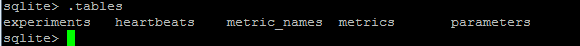
\includegraphics[width=6.0417in,height=0.4791in]{img12.png}


{\selectlanguage{english}
These are the tables where the SQLite module stores the data if we
select \textit{sqlite} as output for the simulation heartbeats and the
data related to the experiment. In general, to enable the use of SQLite
storage, the user has to change the configuration file adding the
{\textquotedblleft}heartbeat{\textquotedblright} line in the options
section, as in the following example (see file
{\textquoteleft}sqlite.in{\textquoteright} in the \texttt{src/examples}
directory):}

\begin{flushleft}
\tablehead{}
\begin{supertabular}{|m{6.29346in}|}
\hline
{\selectlanguage{english}\ttfamily options = \{}

{\selectlanguage{english}\ttfamily \ \ \ \ \ \ \ heartbeat=\{ }

{\selectlanguage{english}\ttfamily
\ \ \ \ \ \ \ \ \ \ \ \ \ \ \ \ \ \ \ \ \ type={\textquotedbl}sqlite{\textquotedbl},
}

{\selectlanguage{english}\ttfamily
\ \ \ \ \ \ \ \ \ \ \ \ \ \ \ \ \ \ \ \ \ dbfile={\textquotedbl}/tmp/test.db{\textquotedbl},
}

{\selectlanguage{english}\ttfamily
\ \ \ \ \ \ \ \ \ \ \ \ \ \ \ \ \ \ \ \ \ experiment\_id=1, }

{\selectlanguage{english}\ttfamily
\ \ \ \ \ \ \ \ \ \ \ \ \ \ \ \ \ \ \ \ \ experiment\_description={\textquotedbl}T1{\textquotedbl}
}

{\selectlanguage{english}\ttfamily
\ \ \ \ \ \ \ \ \ \ \ \ \ \ \ \ \ \ \},}

{\selectlanguage{english}\ttfamily \ \ \ \ \ \}}

\selectlanguage{english}\ttfamily \}\\\hline
\end{supertabular}
\end{flushleft}
{\selectlanguage{english}
\foreignlanguage{english}{In order to get same the data from this DB the
user should first look for the needed metric id:}}

\begin{flushleft}
\tablehead{}
\begin{supertabular}{|m{6.29346in}|}
\hline
\selectlanguage{english}\ttfamily sqlite{\textgreater} select * from
metric\_names where name like
{\textquotesingle}\%dcache.write\_miss\%{\textquotesingle};\\\hline
\end{supertabular}
\end{flushleft}
{\selectlanguage{english}
\foreignlanguage{english}{The user should get the following output:}}


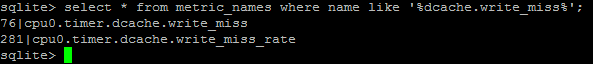
\includegraphics[width=6.1772in,height=0.6665in]{img13.png}


{\selectlanguage{english}
And then look for the associated data in the metrics table using the
{\textquotedblleft}metric\_id{\textquotedblright} values.}

\begin{flushleft}
\tablehead{}
\begin{supertabular}{|m{6.29346in}|}
\hline
\selectlanguage{english}
\foreignlanguage{english}{\texttt{sqlite{\textgreater} select * from
metrics where metric\_id = 76;}}\\\hline
\end{supertabular}
\end{flushleft}
{\selectlanguage{english}
And obtain a long list (here we show only the last three elements):}


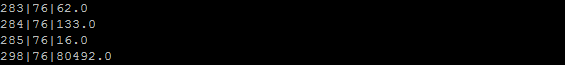
\includegraphics[width=5.8854in,height=0.6772in]{img14.png}


{\selectlanguage{english}
\foreignlanguage{english}{This is where things may not seem clear at
first. The table is organized so that the first n-1 records contain the
value for every sample in the value field. The last one contains the
actual result (in this case the sum of all of the previous records). So
the user can get the actual result with:}}

\begin{flushleft}
\tablehead{}
\begin{supertabular}{|m{6.29346in}|}
\hline
\selectlanguage{english}
\foreignlanguage{english}{\texttt{sqlite{\textgreater} select value
from metrics where metric\_id=76 and heartbeat\_id is (select
max(heartbeat\_id) from metrics);}}\\\hline
\end{supertabular}
\end{flushleft}
{\selectlanguage{english}
\foreignlanguage{english}{The user should be the one showed below, which
should also be the same obtained from the flat file:}}


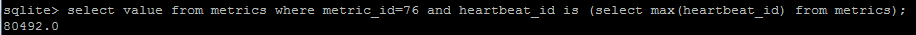
\includegraphics[width=6.2689in,height=0.239in]{img15.png}


{\selectlanguage{english}
\foreignlanguage{english}{As far as the write miss rate is concerned
things, again, change a bit. This time we are
not}\foreignlanguage{english}{ }\foreignlanguage{english}{looking for
the sum but for a rate so we can only get the value directly:}}

\begin{flushleft}
\tablehead{}
\begin{supertabular}{|m{6.29346in}|}
\hline
\selectlanguage{english}
\foreignlanguage{english}{\texttt{sqlite{\textgreater} select value
from metrics where metric\_id=281 and heartbeat\_id is (select
max(heartbeat\_id) from metrics);}}\\\hline
\end{supertabular}
\end{flushleft}
{\selectlanguage{english}
This time the expected values is:}


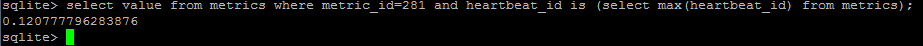
\includegraphics[width=6.2681in,height=0.3118in]{img16.png}


{\selectlanguage{english}
\foreignlanguage{english}{You get more digits from this than from the
flat file because the value field is a
{\textquotedblleft}float8{\textquotedblright}. You can see this by
looking at the table schema:}}

\begin{flushleft}
\tablehead{}
\begin{supertabular}{|m{6.29346in}|}
\hline
\selectlanguage{english}\ttfamily sqlite{\textgreater} .schema
metrics\\\hline
\end{supertabular}
\end{flushleft}
{\selectlanguage{english}
which outputs:}


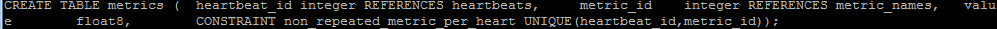
\includegraphics[width=6.272in,height=0.1827in]{img17.png}


\subsubsection[Using a PostgreSQL server:]{\rmfamily Using a PostgreSQL
server:}
{\selectlanguage{english}
\foreignlanguage{english}{While using SQLite can be very convenient as
it gives you the ability to store your heartbeats in a SQL server
without the hassle of configuring a real SQL server it may not be the
best solution if the user wants to store a very big amount of data and
if it wants to offload the burden of saving data to
}\foreignlanguage{english}{another machine. In this case the best
solution, albeit more demanding from the administrator viewpoint, might
be setting up a second computer with PostgreSQL and using it to store
the heartbeats produced by the simulations.}}

{\selectlanguage{english}
\foreignlanguage{english}{As an example in the following the PostgreSQL
server is supposed to run on the same machine running COTSon (note that
the process to run it in a classical client-server configuration is the
same as explained here).}}

{\selectlanguage{english}
\foreignlanguage{english}{As PostgreSQL is not usually installed by
default it is necessary to install it. Type:}}

\begin{flushleft}
\tablehead{}
\begin{supertabular}{|m{6.29346in}|}
\hline
\selectlanguage{english} \foreignlanguage{english}{\texttt{\$
}}\foreignlanguage{english}{\texttt{sudo apt-get --y install postgresql
postgresql-client}}\\\hline
\end{supertabular}
\end{flushleft}
{\selectlanguage{english}
\foreignlanguage{english}{Now the user should have its instance of
PostgreSQL up and running on the specified machine. To verify it, the
user can issue this command:}}

\begin{flushleft}
\tablehead{}
\begin{supertabular}{|m{6.29346in}|}
\hline
\selectlanguage{english}\ttfamily \$ netstat -atp {\textbar} grep
post\\\hline
\end{supertabular}
\end{flushleft}
{\selectlanguage{english}
\foreignlanguage{english}{This should be the output the user obtains:}}


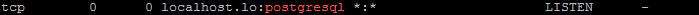
\includegraphics[width=6.2689in,height=0.1339in]{img18.png}


{\selectlanguage{english}
\foreignlanguage{english}{If so then you can start configuring
PostgreSQL to make it talk to COSTon.}}

\subsubsection[Creating the COTSon PostgreSQL database:]{\rmfamily
Creating the COTSon PostgreSQL database:}
{\selectlanguage{english}
\foreignlanguage{english}{In order to configure PostgreSQL the user has
to create the {\textquotedblleft}cotson{\textquotedblright} user in the
database:}}

\begin{flushleft}
\tablehead{}
\begin{supertabular}{|m{6.29346in}|}
\hline
{\selectlanguage{english} \foreignlanguage{english}{\texttt{\$ sudo
--i}}}

{\selectlanguage{english} \foreignlanguage{english}{\texttt{\$ su -
postgres}}}

{\selectlanguage{english}\ttfamily \$ cd}

\selectlanguage{english}\ttfamily \$ createuser cotson\\\hline
\end{supertabular}
\end{flushleft}
{\selectlanguage{english}

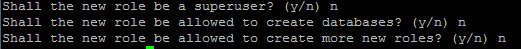
\includegraphics[width=5.4272in,height=0.5102in]{img19.png}
\foreignlanguage{english}{ }}

{\selectlanguage{english}
Answer {\textquotedblleft}NO{\textquotedblright} (n) to the three
questions following this command and then issue:}

\begin{flushleft}
\tablehead{}
\begin{supertabular}{|m{6.29346in}|}
\hline
\selectlanguage{english}\ttfamily \$ createdb cotson -O cotson\\\hline
\end{supertabular}
\end{flushleft}
{\selectlanguage{english}
\foreignlanguage{english}{The user can verify that everything is ok by
querying PostgreSQL and asking for the databases list:}}

\begin{flushleft}
\tablehead{}
\begin{supertabular}{|m{6.29346in}|}
\hline
\selectlanguage{english} \foreignlanguage{english}{\texttt{\$ psql
-l}}\\\hline
\end{supertabular}
\end{flushleft}
{\selectlanguage{english}
The output should be similar to the following}

{\centering\selectlanguage{english}

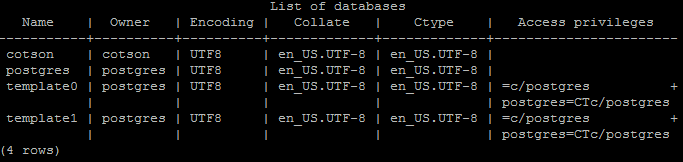
\includegraphics[width=5.9047in,height=1.4035in]{img20.png}
\foreignlanguage{english}{:}
\par}

\subsubsection[Configuring PostgreSQL for COTSon connection:]{\rmfamily
Configuring PostgreSQL for COTSon connection:}
{\selectlanguage{english}
\foreignlanguage{english}{Once the database is ready, the user needs to
configure it, in order to allow incoming connections from COTSon. To do
so the user (still as {\textquoteleft}postgres{\textquoteright} user is
ok) has to modify the following file:}\foreignlanguage{english}{ }}

\begin{flushleft}
\tablehead{}
\begin{supertabular}{|m{6.29346in}|}
\hline
\selectlanguage{english}
\foreignlanguage{english}{\texttt{/etc/postgresql/*/main/pg\_hba.conf}}\\\hline
\end{supertabular}
\end{flushleft}
{\selectlanguage{english}
\foreignlanguage{english}{Becoming root, then the user can change the
file adding the lines highlighted below:}}

\begin{flushleft}
\tablehead{}
\begin{supertabular}{|m{6.29346in}|}
\hline
{\selectlanguage{english}\ttfamily \# TYPE \ DATABASE \ \ \ USER
\ \ \ \ \ \ \ CIDR-ADDRESS \ \ \ \ \ \ \ \ \ METHOD
\ \ \ \ \ \ \ \ \ \ \ \ \ \ \ \ \ \ \ \ \ \ \ \ \ \ \ \ \ \ \ \ \ \ \ \ \ \ \ \ \ \ \ \ \ \ \ \ \ \ \ \ \ \ \ \ \ \ \ \ \ \ \ \ \ \ \ \ \ \ \ \ \ \ \ \ \ \ \ \ \ \ \ \ \ \ \ \ \ \ \ \ \ \ \ \ \ \ \ \ \ \ \ \ \ \ \ \ \ \ \ \ \ \ \ \ \ }

~

{\selectlanguage{english}\ttfamily \#
{\textquotedbl}local{\textquotedbl} is for Unix domain socket
connections only
\ \ \ \ \ \ \ \ \ \ \ \ \ \ \ \ \ \ \ \ \ \ \ \ \ \ \ \ \ \ \ \ \ \ \ \ \ \ \ \ \ \ \ \ \ \ \ \ \ \ \ \ \ \ \ \ \ \ \ \ \ \ \ \ \ \ \ \ \ \ \ \ \ \ \ \ \ \ \ \ \ \ \ \ \ \ \ \ \ \ \ \ \ \ \ \ \ \ \ \ \ \ \ \ \ \ \ \ \ \ \ \ \ \ \ \ \ \ \ \ \ \ \ \ \ }

{\selectlanguage{english}\ttfamily local \ \ all \ \ \ \ \ \ \ \ all
\ \ \ \ \ \ \ \ \ \ \ \ \ \ \ \ \ \ \ \ \ \ \ \ \ \ \ \ \ \ ident}

{\selectlanguage{english}\ttfamily \# IPv4 local connections:
\ \ \ \ \ \ \ \ \ \ \ \ \ \ \ \ \ \ \ \ \ \ \ \ \ \ \ \ \ \ \ \ \ \ \ \ \ \ \ \ \ \ \ \ \ \ \ \ \ \ \ \ \ \ \ \ \ \ \ \ \ \ \ \ \ \ \ \ \ \ \ \ \ \ \ \ \ \ \ \ \ \ \ \ \ \ \ \ \ \ \ \ \ \ \ \ \ \ \ \ \ \ \ \ \ \ \ \ \ \ \ \ \ \ \ \ \ \ \ \ \ \ \ \ \ \ \ \ \ \ \ \ \ \ \ \ \ \ \ \ \ \ \ \ \ \ \ \ \ \ \ \ }

{\selectlanguage{english} \foreignlanguage{english}{\texttt{host
\ \ \ cotson \ \ \ \ \ cotson \ \ \ \ \ \ \ \ \ \ \ \ \ 127.0.0.1/32
\ \ \ \ trust \# add this line in this
place}}\foreignlanguage{english}{\texttt{
\ \ \ \ \ \ \ \ \ \ \ \ \ \ \ \ \ \ \ \ \ \ \ \ \ \ \ \ \ \ \ \ \ \ \ \ \ \ \ \ \ \ \ \ \ \ \ \ \ \ \ \ \ \ \ \ \ \ \ \ \ \ \ \ \ \ \ \ \ \ \ \ \ \ \ \ \ \ \ }}}

{\selectlanguage{english}\ttfamily host \ \ \ all \ \ \ \ \ \ \ \ all
\ \ \ \ \ \ \ \ 127.0.0.1/32 \ \ \ \ \ \ \ \ \ md5}

{\selectlanguage{english}\ttfamily \# IPv6 local connections:
\ \ \ \ \ \ \ \ \ \ \ \ \ \ \ \ \ \ \ \ \ \ \ \ \ \ \ \ \ \ \ \ \ \ \ \ \ \ \ \ \ \ \ \ \ \ \ \ \ \ \ \ \ \ \ \ \ \ \ \ \ \ \ \ \ \ \ \ \ \ \ \ \ \ \ \ \ \ \ \ \ \ \ \ \ \ \ \ \ \ \ \ \ \ \ \ \ \ \ \ \ \ \ \ \ \ \ \ \ \ \ \ \ \ \ \ \ \ \ \ \ \ \ \ \ \ \ \ \ \ \ \ \ \ \ \ \ \ \ \ \ \ \ \ \ \ \ \ \ \ \ \ }

{\selectlanguage{english} \foreignlanguage{english}{\texttt{host
\ \ \ cotson \ \ \ \ \ cotson \ \ \ \ \ \ \ \ ::1/128
\ \ \ \ \ \ \ \ \ \ \ \ \ \ trust \# add this line in this
place}}\foreignlanguage{english}{\texttt{
\ \ \ \ \ \ \ \ \ \ \ \ \ \ \ \ \ \ \ \ \ \ \ \ \ \ \ \ \ \ \ \ \ \ \ \ \ \ \ \ \ \ \ \ \ \ \ \ \ \ \ \ \ \ \ \ \ \ \ \ \ \ \ \ \ \ \ \ \ \ \ \ \ \ \ \ \ \ \ \ \ \ \ \ \ }}}

\selectlanguage{english}\ttfamily host \ \ \ all \ \ \ \ \ \ \ \ all
\ \ \ \ \ \ \ \ ::1/128 \ \ \ \ \ \ \ \ \ \ \ \ \ \ md5\\\hline
\end{supertabular}
\end{flushleft}
{\selectlanguage{english}
\foreignlanguage{english}{Then the last thing to do is to restart the
PostgreSQL server. Still as a root issue the command:}}

\begin{flushleft}
\tablehead{}
\begin{supertabular}{|m{6.29346in}|}
\hline
\selectlanguage{english} \foreignlanguage{english}{\texttt{\$
/etc/init.d/postgresql restart}}\\\hline
\end{supertabular}
\end{flushleft}
{\selectlanguage{english}
Finally:}

\begin{flushleft}
\tablehead{}
\begin{supertabular}{|m{6.29346in}|}
\hline
{\selectlanguage{english} \foreignlanguage{english}{\texttt{\$ psql -d
cotson -U postgres -c {\textquotedbl}GRANT ALL PRIVILEGES ON DATABASE
cotson TO cotson;{\textquotedbl}}}}

\selectlanguage{english} \foreignlanguage{english}{\texttt{\$ psql -d
cotson -U postgres -c {\textquotedbl}ALTER USER cotson WITH PASSWORD
{\textquoteleft}cotson{\textquoteright};{\textquotedblright}}}\\\hline
\end{supertabular}
\end{flushleft}
{\selectlanguage{english}
At this point the user can press two times the
{\textquotedblleft}Ctrl-D{\textquotedblright} to exit the postgres user
shell and the root shell.}


\bigskip

\subsubsection[Creating the PostgreSQL COTSon db
schema:]{\textrm{Creating the
}\foreignlanguage{english}{\textrm{PostgreSQL }}\textrm{COTSon db
schema:}}
{\selectlanguage{english}
\foreignlanguage{english}{Then, there is need for creating the database
structure using the file
{\textquotedblleft}}\foreignlanguage{english}{\texttt{experiment\_definition}}\foreignlanguage{english}{{\textquotedblright}
in the
{\textquoteleft}}\foreignlanguage{english}{\texttt{src/tools/}}\foreignlanguage{english}{{\textquoteright}directory.
}}

\begin{flushleft}
\tablehead{}
\begin{supertabular}{|m{6.29346in}|}
\hline
\selectlanguage{english}\ttfamily \$ cd src/tools\\\hline
\end{supertabular}
\end{flushleft}
{\selectlanguage{english}
We modify for example add the following line at the end of the file,
instead of:}


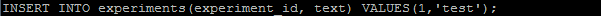
\includegraphics[width=6.2602in,height=0.1665in]{img21.png}


{\selectlanguage{english}
\foreignlanguage{english}{We can write: }}

\begin{flushleft}
\tablehead{}
\begin{supertabular}{|m{6.29346in}|}
\hline
\selectlanguage{english}\ttfamily INSERT INTO
experiments(experiment\_id, description)
VALUES(1,{\textquotesingle}T1{\textquotesingle});\\\hline
\end{supertabular}
\end{flushleft}
{\selectlanguage{english}
\foreignlanguage{english}{Then we can enter again the DB with:}}

\begin{flushleft}
\tablehead{}
\begin{supertabular}{|m{6.29346in}|}
\hline
\selectlanguage{english} \foreignlanguage{english}{\texttt{\$ psql -h
localhost -d cotson -U cotson}}\\\hline
\end{supertabular}
\end{flushleft}
{\selectlanguage{english}
At the prompt, provide the password
{\textquoteleft}cotson{\textquoteright}}

{\selectlanguage{english}
To setup the database schema:}

\begin{flushleft}
\tablehead{}
\begin{supertabular}{|m{6.29346in}|}
\hline
\selectlanguage{english} \foreignlanguage{english}{\texttt{Postgres=\#
{\textbackslash}i experiments\_definition}}\\\hline
\end{supertabular}
\end{flushleft}
{\selectlanguage{english}
\foreignlanguage{english}{This should output:}}


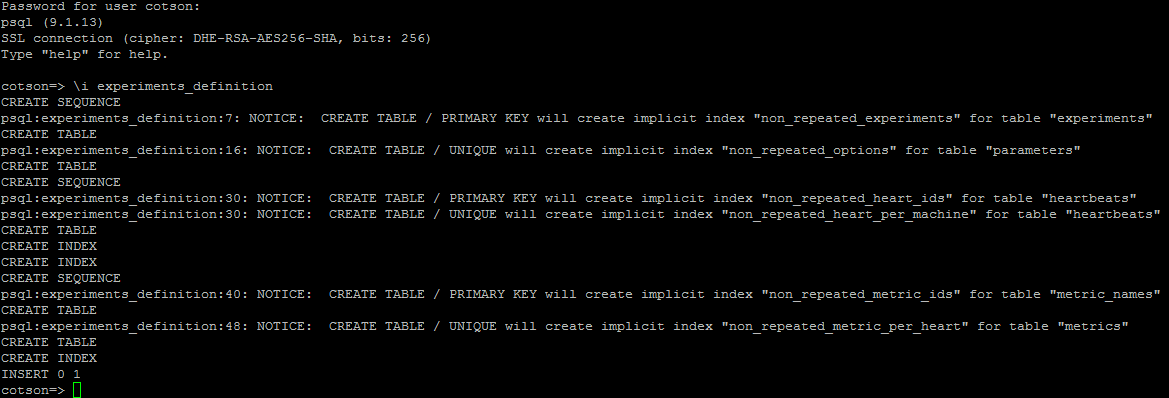
\includegraphics[width=6.2709in,height=2.1346in]{img22.png}


{\selectlanguage{english}
Then we return to the shell with
{\textquotedblleft}Ctrl-D{\textquotedblright}.}

\subsubsection[Modifying the {\textquotedblleft}.in{\textquotedblright}
file to save our heartbeats in PostgreSQL:]{\rmfamily Modifying the
{\textquotedblleft}.in{\textquotedblright} file to save our heartbeats
in PostgreSQL:}
{\selectlanguage{english}
\foreignlanguage{english}{At this point the configuration phase is
completed. To check that this works, we can modify the sqlite.in
example as follows:}}

\begin{flushleft}
\tablehead{}
\begin{supertabular}{|m{6.29346in}|}
\hline
{\selectlanguage{english}\ttfamily \$ cd src/examples}

\selectlanguage{english}\ttfamily \$ cp sqlite.in pgsql.in\\\hline
\end{supertabular}
\end{flushleft}
{\selectlanguage{english}
\foreignlanguage{english}{Then we can modify the file
{\textquotedblleft}pgsql.in{\textquotedblright}, by changing the
heartbeat type from {\textquotedblleft}sqlite{\textquotedblright} to
{\textquotedblleft}pgsql{\textquotedblright} and setup the
{\textquotedblleft}dbconn={\dots}{\textquotedblright} line as shown
below:}}

\begin{flushleft}
\tablehead{}
\begin{supertabular}{|m{6.29346in}|}
\hline
{\selectlanguage{english}
\foreignlanguage{english}{\texttt{\ \ \ \ \ \ \ \ }}\foreignlanguage{english}{\texttt{heartbeat
= \{}}}

{\selectlanguage{english}\ttfamily
\ \ \ \ \ \ \ \ \ \ \ \ \ \ \ \ type={\textquotedbl}pgsql{\textquotedbl},}

{\selectlanguage{english}\ttfamily
\ \ \ \ \ \ \ \ \ \ \ \ \ \ \ \ dbconn={\textquotedbl}host=localhost
dbname=cotson user=cotson password=cotson{\textquotedbl},}

{\selectlanguage{english}\ttfamily
\ \ \ \ \ \ \ \ \ \ \ \ \ \ \ \ experiment\_id=EXP,}

{\selectlanguage{english}
\foreignlanguage{english}{\texttt{\ \ \ \ \ \ \ \ \ \ \ \ \ \ \ \ }}\foreignlanguage{english}{\texttt{experiment\_description={\textquotedbl}T1{\textquotedblright}}}}

\selectlanguage{english}
\foreignlanguage{english}{\texttt{\ \ \ \ \ \ \ \ }}\foreignlanguage{english}{\texttt{\},}}\foreignlanguage{english}{\texttt{\}}}\\\hline
\end{supertabular}
\end{flushleft}
\subsubsection[Running COTSon with PostgreSQL]{\textrm{Running COTSon
with PostgreSQ}\foreignlanguage{english}{\textrm{L}}}
{\selectlanguage{english}
\foreignlanguage{english}{Now, the user is ready to run a complete
experiment on COTSon and stores the collected statistics in the
PostgreSQL database server. }}

\begin{flushleft}
\tablehead{}
\begin{supertabular}{|m{6.29346in}|}
\hline
\selectlanguage{english} \foreignlanguage{english}{\texttt{\$
}}\ \foreignlanguage{english}{\texttt{../../bin/cotson
pgsql.in}}\\\hline
\end{supertabular}
\end{flushleft}
{\selectlanguage{english}
\foreignlanguage{english}{The user should be aware that using PostgreSQL
server on the same machine can be painful slow. As a rule of thumb, the
user should expect that flat files are the fastest way to save your
data, there is SQLite server as a middle speed solution, while
PostgreSQL server (on the same machine) is the slowest option.}}

\section[Simple Examples]{Simple Examples}
{\selectlanguage{english}
All the examples that will be refer to, can be found in the following
path: }

\begin{flushleft}
\tablehead{}
\begin{supertabular}{|m{6.21846in}|}
\hline
\selectlanguage{english}\ttfamily cotson/src/examples\\\hline
\end{supertabular}
\end{flushleft}
{\selectlanguage{english}
A more complete verification test can be launched by typing the
following command:}

\begin{flushleft}
\tablehead{}
\begin{supertabular}{|m{6.21846in}|}
\hline
\selectlanguage{english}\ttfamily \$ make run\\\hline
\end{supertabular}
\end{flushleft}
{\selectlanguage{english}
In this case, several examples contained in the example folder are
sequentially executed. Following this verification procedure, the
reader can see different examples executing, each of them targeting a
specific feature of the simulator.}

{\selectlanguage{english}
From this folder, the user can also run a specific example that have
been setup through the Makefile, by typing the following command:}

\begin{flushleft}
\tablehead{}
\begin{supertabular}{|m{6.21846in}|}
\hline
\selectlanguage{english} \texttt{\$ make
run\_}\texttt{\textit{name\_of\_the\_example}}\\\hline
\end{supertabular}
\end{flushleft}
{\selectlanguage{english}
Where the string \texttt{\textit{name\_of\_the\_example }}identifies the
file name associated to the example (type {\textquotedblleft}ls
*.in{\textquotedblright} to see names of possible examples. E.g., for
running the {\textquotedblleft}functional.in{\textquotedblright}
example type:}

\begin{flushleft}
\tablehead{}
\begin{supertabular}{|m{6.20526in}|}
\hline
\selectlanguage{english} \texttt{\$ make
run\_}\texttt{\textit{functional}}\\\hline
\end{supertabular}
\end{flushleft}
\subsection[Functional Simulation example (functional.in)]{Functional
Simulation\foreignlanguage{english}{ example (functional.in)}}
{\selectlanguage{english}
As said in the first part of the guide, a functional simulation
doesn{\textquotesingle}t use timing at all. For this reason it is very
fast but assuming an ideal
({\textquotedblleft}CPI=1{\textquotedblright} timing model). Here, the
Lua file \textit{functional.in} (see Fig. 12 below) that will be used.}

{\centering 
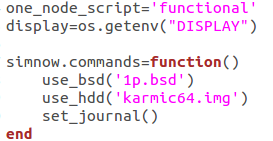
\includegraphics[width=2.35in,height=1.2138in]{img23.png}
\par}

{\centering\selectlanguage{english}\sffamily\bfseries
\label{bkm:Ref388170548}Fig.
\stepcounter{Figure}{\theFigure} -- Lua configuration file for running
a pure functional simulation with COTSon.
\par}

\subsubsection[Goal of the experiment or example]{\rmfamily Goal of the
experiment or example}
{\selectlanguage{english}
As can be seen in the previous figure, in the script there is the option
{\textquotedblleft}\textit{one\_node\_script={\dots}{\textquotedblright}}
that tells COTSon to refer to a template
{\textquotedblleft}functional{\textquotedblright}, which contains
default options for running a functional simulation. The second line of
the code is needed to display the SimNow Graphical User Interface.
Then, there are the SimNow commands that allow the user to choose the
bsd and hdd by inserting their absolute paths or otherwise by placing
the desired bsd and hdd in the directory cotson/data.}

\subsubsection[Location of the involved files]{\rmfamily Location of the
involved files}
{\selectlanguage{english}
All the files needed to run the example are contained in the following
folder:}

\begin{flushleft}
\tablehead{}
\begin{supertabular}{|m{6.21846in}|}
\hline
\selectlanguage{english}
\texttt{\$COTSONHOME}\foreignlanguage{english}{\texttt{/src/examples}}\\\hline
\end{supertabular}
\end{flushleft}
{\selectlanguage{english}
Where \$\textbf{COTSONHOME }is an environment variable identifying the
installation path of the COTSon simulator.}

\subsubsection[Detailed instructions to start]{\rmfamily Detailed
instructions to start}
{\selectlanguage{english}
\ To run one example, move on the following folder and launch the
simulator:}

\begin{flushleft}
\tablehead{}
\begin{supertabular}{|m{6.21846in}|}
\hline
{\selectlanguage{english}\ttfamily \$ cd src/examples}

\selectlanguage{english} \texttt{\$ make run\_functional}\\\hline
\end{supertabular}
\end{flushleft}
{\selectlanguage{english}
To start the simulation it is necessary to press the start button
(circled in red in Fig. 13 -- see subsection 6.1.4). At this point the
simulation has started and the prompt of the guest (emulated) machine
can be used. }

\subsubsection[Expected output]{\rmfamily Expected output}
{\selectlanguage{english}
After launching the application the graphical user interface should
appear as follows:}


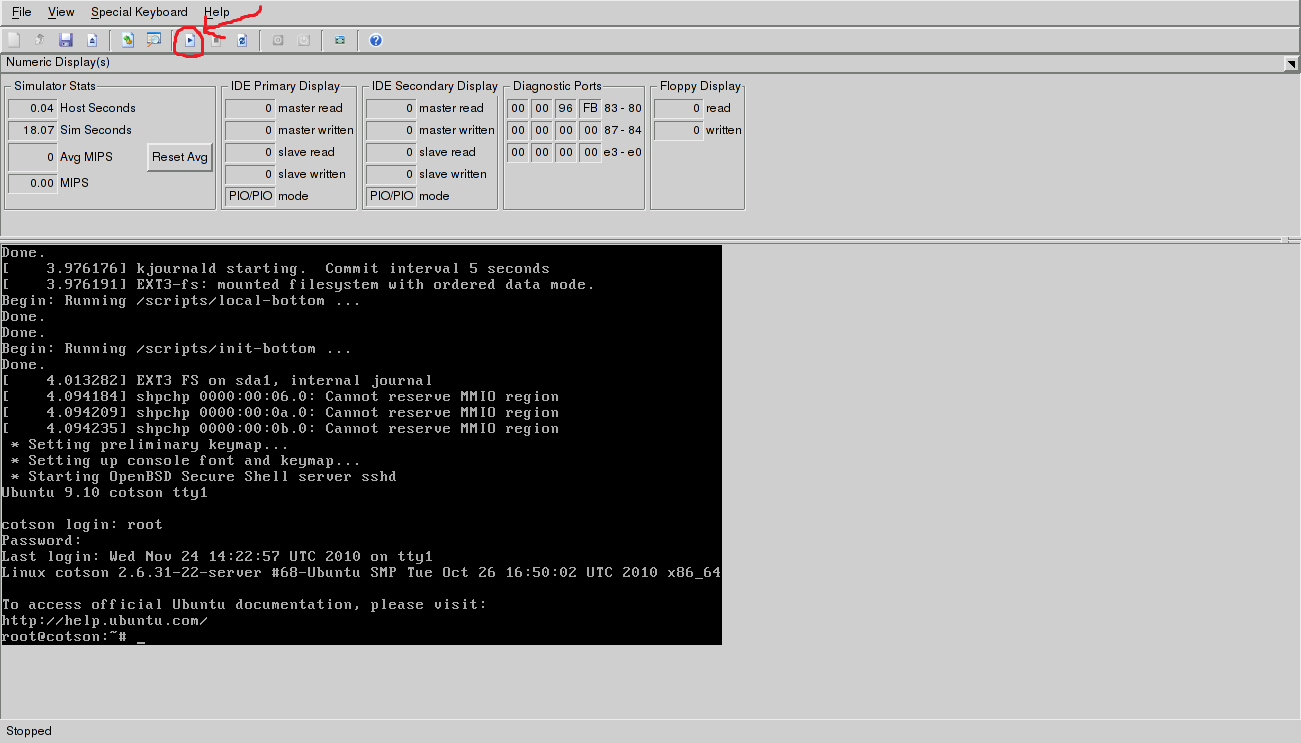
\includegraphics[width=6.2602in,height=3.5673in]{img24.png}


{\centering\selectlanguage{english}\sffamily\bfseries
\label{bkm:Ref388170568}Fig.
\stepcounter{Figure}{\theFigure} -- Expected output for the
{\textquotedblleft}functional.in{\textquotedblright} example
\par}

\subsection[Memory tracing example
(mem\_tracer.in)]{\selectlanguage{english} Memory tracing example
(mem\_tracer.in)}
{\selectlanguage{english}
To analyze in detail the performance of a system, it is often useful to
record a trace of the references that are flowing through the system.
This is supported in COTSon through the
{\textquotedblleft}tracers{\textquotedblright}. In the
{\textquotedblleft}mem\_tracer.in{\textquotedblright} example we can
see how to setup a tracer.}

{\centering 
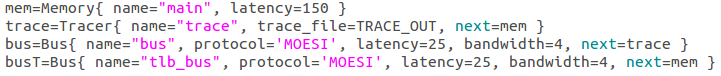
\includegraphics[width=6.2709in,height=0.6575in]{img25.png}
\par}

{\centering\selectlanguage{english}\sffamily\bfseries
\label{bkm:Ref388170583}Fig.
\stepcounter{Figure}{\theFigure} -- Relevant lines of the Lua
configuration file for the memory tracer example. In this case the lua
script contains another variable (not shown here) that sets
TRACE\_FILE={\textquotedblright}/tmp/mem\_tracer.txt.gz{\textquotedblright}
\par}

\subsubsection[Goal of the experiment or example]{\rmfamily Goal of the
experiment or example}
{\selectlanguage{english}
Memory tracing is achieved by placing a transparent object that
intercepts every memory request and dumps this information to a file
for further analysis. This is how it is specified in the example
\textbf{mem\_tracer.in}. The
{\textquotedblleft}\textit{trace={\textquotedblright}} option inside
the \textit{build} function specifies to intercept every access to the
main memory. The tracer is not only limited to the main memory, it is
also possible to intercept a request to any memory unit in the memory
hierarchy. Simply placing the tracer before L2 or L1 cache, it is
possible to intercept every access to the respective cache. A memory
tracer is added to the memory hierarchy through the line (see also Fig.
14):}

\begin{flushleft}
\tablehead{}
\begin{supertabular}{|m{6.21846in}|}
\hline
\selectlanguage{english} \texttt{trace=Tracer\{
name={\textquotedblright}{\dots}{\textquotedblright},
trace\_file={\textquotedblright}{\dots}{\textquotedblright},
next={\textquotedblright}{\dots}{\textquotedblright}\}}\\\hline
\end{supertabular}
\end{flushleft}

The tracer is defined inside the \textit{build} function of the Lua
configuration script. Its parameters must be defined in a Lua table
called \textit{Tracer}. This table has three fields: (i) the field
\textit{name} specifies the name of the {\textquotedblleft}tracer
object{\textquotedblright}, (ii) the field \textit{trace\_file}
specifies the file where the trace output is dumped, and (iii) the
field \textit{next} specifies the name of the memory unit whose access
is intercepted by the tracer. As mentioned above, this type of objects
can be placed in any position of the memory hierarchy to trace
different hardware blocks. In the example \textit{mem\_tracer.in} it is
placed just before the main memory (setting next=mem), so it will
record each memory access in a file, specified by writing:

\begin{flushleft}
\tablehead{}
\begin{supertabular}{|m{6.21846in}|}
\hline
\selectlanguage{english}
\texttt{trace\_file={\textquotesingle}}\texttt{\textit{path\_of\_the\_file}}\texttt{{\textquotesingle}}\\\hline
\end{supertabular}
\end{flushleft}

The output of the tracer is a gzip compressed text file. A line in the
output corresponds to a single memory access where each line is
composed of five fields. The first field is a time-stamp of the access,
the second field indicates the access type, i.e.,
{\textquotesingle}r{\textquotesingle} for read and
{\textquotesingle}w{\textquotesingle} for write, the third and fourth
fields indicate the physical and virtual addresses, respectively;
finally, the fifth field specifies from the cpu where the access is
originated and the type of transactions generated at each level of the
memory hierarchy (see Fig. 15).

\subsubsection[Location of the involved files]{\rmfamily Location of the
involved files}
{\selectlanguage{english}
All the files needed to run the example are contained in the following
folder:}

\begin{flushleft}
\tablehead{}
\begin{supertabular}{|m{6.21846in}|}
\hline
\selectlanguage{english}
\texttt{\$COTSONHOME}\foreignlanguage{english}{\texttt{/src/examples}}\\\hline
\end{supertabular}
\end{flushleft}
{\selectlanguage{english}
Where \$\textbf{COTSONHOME }is an environment variable identifying the
installation path of the COTSon simulator.}

\subsubsection[Detailed instructions to start]{\rmfamily Detailed
instructions to start}
{\selectlanguage{english}
\ To run the example, move on the example folder and then run the
example as follows:}

\begin{flushleft}
\tablehead{}
\begin{supertabular}{|m{6.21846in}|}
\hline
{\selectlanguage{english}\ttfamily \$ cd src/examples}

\selectlanguage{english} \texttt{\$ make run\_mem\_tracer}\\\hline
\end{supertabular}
\end{flushleft}
\subsubsection[Expected output]{\rmfamily Expected output}
{\selectlanguage{english}
After launching the application the following trace is produced by the
program, and displayed on the host shell:}


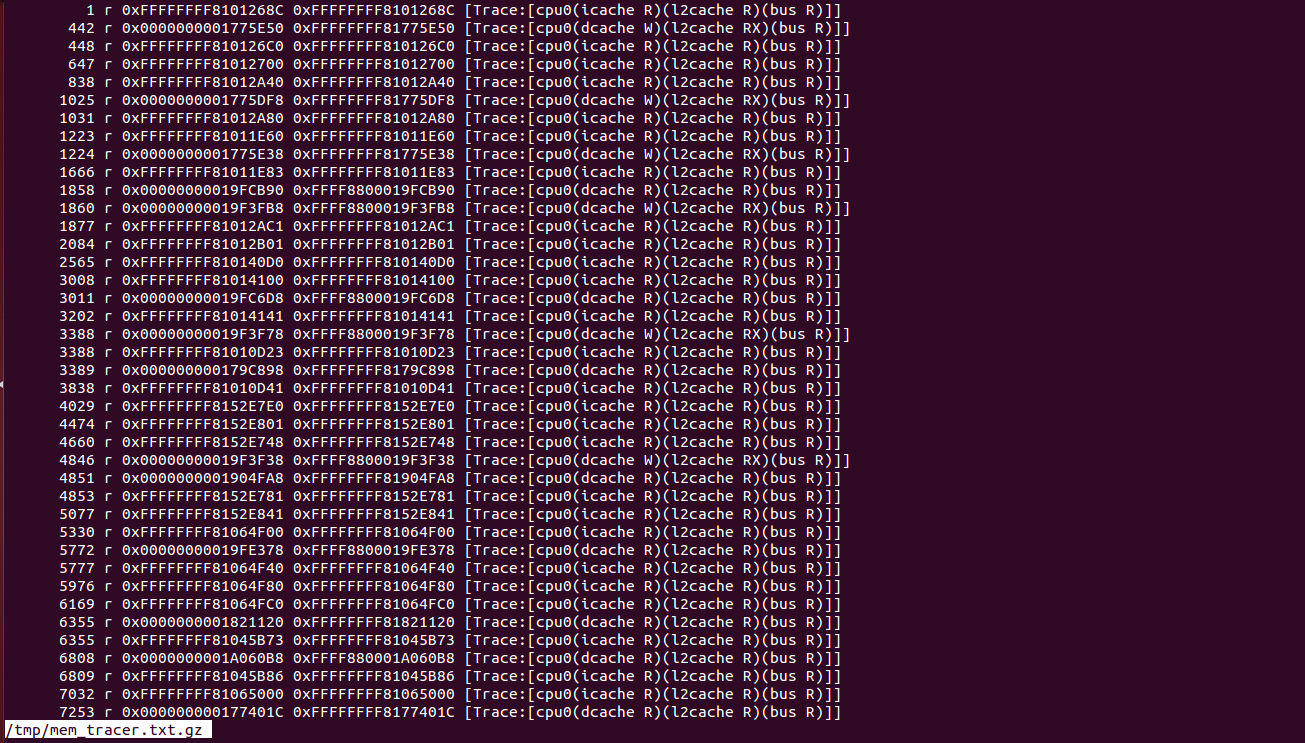
\includegraphics[width=6.2661in,height=3.5673in]{img26.png}


{\centering\selectlanguage{english}\sffamily\bfseries
\label{bkm:Ref388193842}Fig.
\stepcounter{Figure}{\theFigure} -- Expected output for the memory
trace simulation with COTSon simulator.
\par}

{\selectlanguage{english}
The same result can be found in the host file:}

\begin{flushleft}
\tablehead{}
\begin{supertabular}{|m{6.21846in}|}
\hline
\selectlanguage{english}\ttfamily /tmp/mem\_tracer.txt.gz\\\hline
\end{supertabular}
\end{flushleft}
{\selectlanguage{english}
As can be seen in the Lua configuration file \textit{mem\_tracer.in},
the chosen sampler is of type interval, meaning that a timing
simulation is done after fixed intervals of time, and has a fixed
duration (more details on samplers are in Section 6.3). During the
simulation, for each sample the time elapsed from the beginning of the
simulation and the calculated IPC are printed on the shell screen (see
below).}

{\centering 
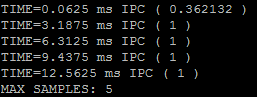
\includegraphics[width=2.1736in,height=0.8201in]{img27.png}
\par}

{\selectlanguage{english}
Modification to the sampling policy is available in the examples
\textit{trace\_stats.in} and \textit{mem\_tracer2.in.} Here, the traces
are obtained by changing the type of the CPU{\textquotesingle}s timer
(see Fig. 16) and setting
TRACE\_OUT={\textquotesingle}/tmp/mem\_tracer.txt.gz{\textquotesingle}.}

{\centering 
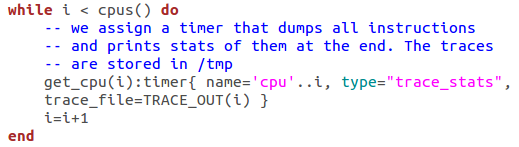
\includegraphics[width=4.011in,height=1.1283in]{img28.png}
\par}

{\centering\selectlanguage{english}\sffamily\bfseries
\label{bkm:Ref388170597}Fig.
\stepcounter{Figure}{\theFigure} -- Lua configuration file for setting
the timer to trace\_stats.in example
\par}

{\selectlanguage{english}
The trace\_stats is in this case a
{\textquotedblleft}fake{\textquotedblright} CPU timer (see
{\textquoteleft}./abaeterno/timer\_cpu/trace\_stats.cpp{\textquoteright}
for more details) that prints some trace statistics in the specified
file. The output on the host screen in this case is:}

{\centering 
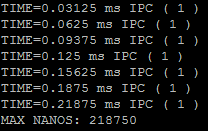
\includegraphics[width=1.8736in,height=1.1827in]{img29.png}
\par}

{\selectlanguage{english}
While the trace file shows a detailed disassembly of the instructions:}

{\centering 
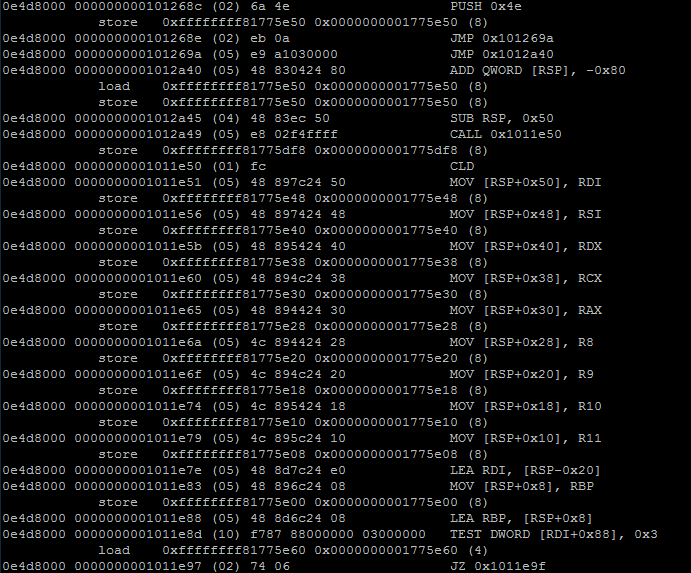
\includegraphics[width=4.6134in,height=3.8256in]{img30.png}
\par}

{\selectlanguage{english}
In the case of \textit{mem\_tracer2.in} example (see Fig. 17 below) the
{\textquotedblleft}fake{\textquotedblright} timer is
{\textquotedblleft}memtracer (see
{\textquoteleft}./abaeterno/timer\_cpu/memory\_tracer.cpp for more
details). }

{\centering 
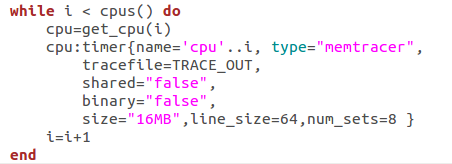
\includegraphics[width=3.3846in,height=1.228in]{img31.png}
\par}

{\centering\selectlanguage{english}\sffamily\bfseries
\label{bkm:Ref388170603}Fig.
\stepcounter{Figure}{\theFigure} - Lua configuration file for setting
the timer to mem\_tracer2.in example.
\par}

{\selectlanguage{english}
The output on the screen is:}

{\centering 
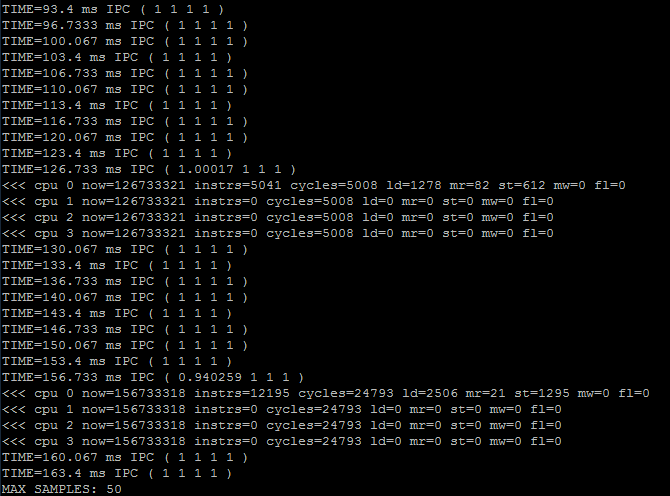
\includegraphics[width=4.7102in,height=3.4874in]{img32.png}
\par}

{\selectlanguage{english}
And the content of trace file is:}

{\centering 
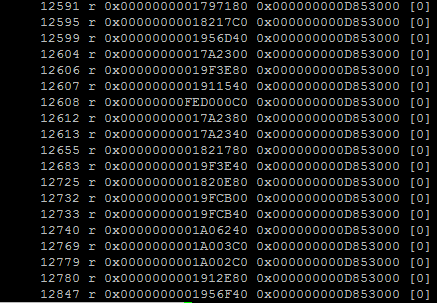
\includegraphics[width=3.172in,height=2.1992in]{img33.png}
\par}

{\selectlanguage{english}
The values in this case represent in order: i) the number of nanoseconds
(timestamp), ii) he type of operation (r for read, w for write), iii)
the address involved, iv) the content of the x86 CR3 register, and v)
the cpu identifier.}

\subsubsection[Defining the Region Of Interest
(ROI)]{\foreignlanguage{english}{\textrm{Defining the Region Of
Interest (ROI)}}}
{\selectlanguage{english}
Although the discussion of how to setup a the Region Of Interest is
presented as part of a tracer example, the technique is general and
serves to measure metrics related to the portion of the code that is
marked by the user.}

{\selectlanguage{english}\ttfamily
\textrm{COTSon comes with the capability of timing simulation of a
specific part of a benchmark, hereafter referred to as
}\textrm{\textit{Region Of Interest}}\textrm{ (ROI). Currently this is
achieved in two ways, the first one is to enable the timing just before
the benchmark starts and to disable it right after the benchmark
finishes. This approach considers the whole benchmark as the ROI. The
second approach is to mark a portion of the benchmark for which a
timing simulation is required. A practical example of the first
approach is provided inside }\textrm{\textit{src/examples/tracer/
}}\textrm{(see }\textrm{Fig. 18}\textrm{).}}

{\centering 
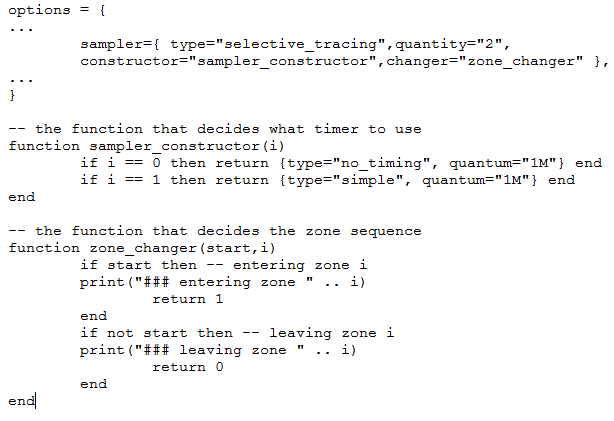
\includegraphics[width=3.6264in,height=2.4862in]{img34.png}
\par}

{\centering\selectlanguage{english}\sffamily\bfseries
\label{bkm:Ref388197251}Fig.
\stepcounter{Figure}{\theFigure} -- The definition of the ROI in the
example cotson\_tracer.in
\par}

{\selectlanguage{english}\ttfamily
\textrm{To achieve this, the sampler to be used must be of type
{\textquotedblleft}}\textrm{\textit{selective\_tracing{\textquotedblright}}}\textrm{,
which in essence is a collection of other samplers, each of which is
used when a certain condition is met during the entire simulation. For
the specific scenario, the selective sampler is composed of two
samplers: }\textrm{\textit{no\_timing}}\textrm{ and
}\textrm{\textit{simple}}\textrm{. In this case, the simulation runs in
a timing mode or in functional mode until a certain trigger is given by
the application (see below), then another trigger stops the timing
simulation, therefore freezing the timing statistics update. }}

{\selectlanguage{english}\ttfamily
\textrm{The configuration file
}\textrm{\textit{cotson\_tracer.in}}\textrm{ (}\textrm{Fig.
18}\textrm{) is an example, which shows how these parameters are
specified. }\textrm{\textit{run.sh}}\textrm{ is the script that
executes inside SimNow (since it is specified by the
{\textquotedblleft}execute({\textquoteleft}run.sh{\textquoteright}){\textquotedblright}
simnow.commands function) and it contains specific commands (or
{\textquotedblleft}triggers{\textquotedblright}) to mark the start and
the end of the timing simulation. This requires that the selected
hard-disk image (hdd) provides the
{\textquoteleft}cotson\_tracer{\textquoteright} executable (this is the
case for the {\textquotedblleft}karmic64,img{\textquotedblright} hdd
that comes by default with COTSon) \ essentially, the
}\textrm{\textit{cotson\_tracer}}\textrm{ is an helper program that
takes three arguments and is supposed to be used inside the execution
script as in the following format:}}

\begin{flushleft}
\tablehead{}
\begin{supertabular}{|m{6.21846in}|}
\hline
{\selectlanguage{english}\ttfamily
cotson\_tracer 10 1 0}

{\selectlanguage{english}\ttfamily
./benchmark}

\selectlanguage{english}\ttfamily
cotson\_tracer 10 1 1\\\hline
\end{supertabular}
\end{flushleft}
{\selectlanguage{english}
The first argument specifies the type of the sampler used, number 10 is
reserved for \textit{selective\_tracing}. The second argument is an
integer value used as an identification of the simulation zone for
which timing simulation is enable/disabled (in this case this indicates
{\textquotedblleft}Zone 1{\textquotedblright}). Finally, the third
argument is a switch to enable/disable the timing simulation. Hence,
cotson\_tracer 10 1 0 implies that timing is enabled for zone 1 and
cotson\_tracer 10 1 1 implies that timing is disabled for zone 1.}

{\selectlanguage{english}
A finer grain control is possible too. In this case, the steps are the
following:}

\begin{enumerate}
\item {\selectlanguage{english}
The user as to include the
{\textquotedblleft}cotson\_tracer.h{\textquotedblright} header provided
in the src/example/tracer directory;}
\item {\selectlanguage{english}
The user can then mark the portion of code of interest (ROI) with a
COTSON\_INTERNAL(10,1,0) to start the timing simulation for
{\textquotedblleft}Zone 1{\textquotedblright} and
COTSON\_INTERNAL(10,1,1) to stop the timing simulation for
{\textquotedblleft}Zone 1{\textquotedblright};}
\end{enumerate}
{\selectlanguage{english}
Note that, in this case, it is not necessary to have the
{\textquotedblleft}cotson\_tracer{\textquotedblright} helper program in
the hdd image.}

\subsection[Samplers: timing simulation]{Samplers: timing simulation}
\label{bkm:Ref388194089}\label{bkm:Ref388175073}\label{bkm:Ref388175045}{\selectlanguage{english}
There are several types of samplers available (check their
implementations in the folder cotson/src/abaeterno/sampler). Here we
discuss more details about the following four samplers:}

\begin{itemize}
\item {\selectlanguage{english}
\textbf{simple}: timing simulation is always on. For example this type
of sampler is used in the example configuration
\textit{one\_cpu\_simple.in};}
\item {\selectlanguage{english}
\textbf{interval}: the duration of each phase (state) of the sampling
(functional, warming, simulation) is fixed. This type of sampler is
used in the example configuration in
\textit{multiple\_cpu\_interval.in};}
\item {\selectlanguage{english}
\textbf{dynamic}: the sample intervals are determined dynamically by the
sampler according to the variation of a monitored variable This type of
sampler is used in the example configuration in \textit{dynamic.in};}
\item {\selectlanguage{english}
\textbf{SMARTS:} the duration of each phase (state) of the sampling
(functional, warming, simulation) is fixed, but the sampling instants
are determined by a previous profiling phase. This type of sampler is
used in the example configuration in \textit{smarts.in};}
\end{itemize}
{\selectlanguage{english}
To specify the full timing simulation the lua file contains the
following (see file \textit{one\_cpu\_simple.in}):}

\begin{flushleft}
\tablehead{}
\begin{supertabular}{|m{6.21846in}|}
\hline
\selectlanguage{english}\ttfamily sampler=\{
type={\textquotedbl}simple{\textquotedbl},
quantum={\textquotedbl}100k{\textquotedbl} \}, -{}- quantum is in
cycles\\\hline
\end{supertabular}
\end{flushleft}
{\selectlanguage{english}
To specify the interval based simulation, where the execution takes
systematically a given amount of time for the functional, warming and
timing simulation, the lua file contains the following (see file
\textit{multiple\_cpu\_interval.in}):}

\begin{flushleft}
\tablehead{}
\begin{supertabular}{|m{6.21846in}|}
\hline
{\selectlanguage{english}\ttfamily sampler=\{
type={\textquotedbl}interval{\textquotedbl},
functional={\textquotedbl}1M{\textquotedbl},
warming={\textquotedbl}100k{\textquotedbl},
simulation={\textquotedbl}100k{\textquotedbl}, \},}

{\selectlanguage{english}\ttfamily
\ \ \ \ \ \ \ \ \ \ \ \ \ \ \ \ {}-{}- the sampler will execute
warming, simulation and then functional for}

{\selectlanguage{english}\ttfamily
\ \ \ \ \ \ \ \ \ \ \ \ \ \ \ \ {}-{}- their respective interval
lengths. After the first simulation sample,}

\selectlanguage{english}
\texttt{\ \ \ \ \ \ \ \ \ \ \ \ \ \ \ \ }\texttt{{}-{}- though it will
finish (due to max\_samples being 1)}\\\hline
\end{supertabular}
\end{flushleft}
{\selectlanguage{english}
To specify the interval based simulation, where the execution takes
systematically a given amount of time for the functional, warming and
timing simulation, the lua file contains the following (see file
\textit{smarts.in}); this is similar to the {\textquotedblleft}interval
sampling{\textquotedblright} but in this case a profiling phase is also
required{\textquotedblright}:}

\begin{flushleft}
\tablehead{}
\begin{supertabular}{|m{6.21846in}|}
\hline
{\selectlanguage{english}\ttfamily sampler=\{
type={\textquotedbl}smarts{\textquotedbl},
functional={\textquotedbl}100k{\textquotedbl},
warming={\textquotedbl}100k{\textquotedbl},
simulation={\textquotedbl}100k{\textquotedbl}, \},}

{\selectlanguage{english}\ttfamily
\ \ \ \ \ \ \ \ \ \ \ \ \ \ \ \ {}-{}- the sampler will execute
warming, simulation and then functional for}

\selectlanguage{english}\ttfamily \ \ \ \ \ \ \ \ \ \ \ \ \ \ \ \ {}-{}-
their respective interval lengths until reaching 1M nanos\\\hline
\end{supertabular}
\end{flushleft}
{\selectlanguage{english}
To specify the dynamic based simulation, where the execution is switched
to full timing according to phases that are detected through an
{\textquotedblleft}non-timing{\textquotedblright} variable (in this
case the variable is the number of exceptions on any cpu simulated),
the lua file contains the following (see file \textit{dynamic.in}):}

\begin{flushleft}
\tablehead{}
\begin{supertabular}{|m{6.21846in}|}
\hline
{\selectlanguage{english}\ttfamily sampler=\{
type={\textquotedbl}dynamic{\textquotedbl},
functional={\textquotedbl}100k{\textquotedbl},
warming={\textquotedbl}100k{\textquotedbl},
simulation={\textquotedbl}100k{\textquotedbl},}

{\selectlanguage{english}\ttfamily
\ \ \ \ \ \ \ \ \ \ \ \ \ \ \ \ \ \ maxfunctional=10,
sensitivity={\textquotedbl}90{\textquotedbl},}

{\selectlanguage{english}\ttfamily
\ \ \ \ \ \ \ \ \ \ \ \ \ \ \ \ \ \ variable=\{{\textquotedbl}cpu.*.other\_exceptions{\textquotedbl}\},
\},}

{\selectlanguage{english}\ttfamily
\ \ \ \ \ \ \ \ \ \ \ \ \ \ \ \ {}-{}- the sampler will execute
warming, simulation and then functional for}

\selectlanguage{english}\ttfamily \ \ \ \ \ \ \ \ \ \ \ \ \ \ \ \ {}-{}-
their respective interval lengths until reaching 1M nanos\\\hline
\end{supertabular}
\end{flushleft}
{\selectlanguage{english}
The length of the intervals, where functional, warming, full-timing
simulation is performed, is specified in a way similar to the interval
simulation. If the first-derivative of this variable goes beyond the
sensitivity (set by the line
\textit{sensitivity={\textquotedblright}90{\textquotedblright}}) there
is a phase change in the program and so a timing simulation can start.
The variable
\textit{maxfunctional={\textquotedblright}10{\textquotedblright}} is
needed to set the maximum number of time intervals passed in the
functional state before a new timing simulation starts. This type of
sampler is used in dynamic.in. As you can see from Fig. 20 the
intervals between the printed values of time are not regular but they
are variable.}

\subsubsection[Goal of the experiment or example]{\rmfamily Goal of the
experiment or example}
{\selectlanguage{english}
The main purpose of the example is the illustration of the use of
different sampler.}

\subsubsection[Location of the involved files]{\rmfamily Location of the
involved files}
{\selectlanguage{english}
All the files needed to run the example are contained in the following
folder:}

\begin{flushleft}
\tablehead{}
\begin{supertabular}{|m{6.21846in}|}
\hline
\selectlanguage{english}
\texttt{\$COTSONHOME}\foreignlanguage{english}{\texttt{/src/examples}}\\\hline
\end{supertabular}
\end{flushleft}
{\selectlanguage{english}
where \$\textbf{COTSONHOME }is an environment variable identifying the
installation path of the COTSon simulator.}

\subsubsection[Detailed instructions to start for NO Sampling
({\textquotedblleft}simple{\textquotedblright})]{\textrm{Detailed
instructions to start}\foreignlanguage{english}{\textrm{ for NO
Sampling ({\textquotedblleft}simple{\textquotedblright})}}}
{\selectlanguage{english}
\ To run the example, move on the example folder and then run the
example as follows:}

\begin{flushleft}
\tablehead{}
\begin{supertabular}{|m{6.21846in}|}
\hline
{\selectlanguage{english}\ttfamily \$ cd src/examples}

\selectlanguage{english} \texttt{\$ make
run\_one\_cpu\_simple.in}\\\hline
\end{supertabular}
\end{flushleft}
\subsubsection[Expected output for NO Sampling
({\textquotedblleft}simple{\textquotedblright})]{\textrm{Expected
output}\foreignlanguage{english}{\textrm{ for NO Sampling
({\textquotedblleft}simple{\textquotedblright})}}}
{\selectlanguage{english}
After launching the application the following output should be obtained
(see Fig. 21). In this case, the timing simulation is always on:}

{\centering 
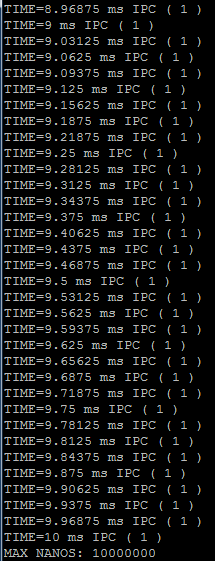
\includegraphics[width=1.4756in,height=3.8563in]{img35.png}
\par}

{\centering\selectlanguage{english}\sffamily\bfseries
Fig.
\stepcounter{Figure}{\theFigure} -- Expected output for
{\textquotedblleft}simple{\textquotedblright} sampler example. The
example is based on the one\_cpu\_simple.in Lua configuration file.
\par}

\subsubsection[Detailed instructions to start for Dynamic
Sampling]{\textrm{Detailed instructions to
start}\foreignlanguage{english}{\textrm{ for Dynamic Sampling}}}
{\selectlanguage{english}
\ To run the example, move on the example folder and then run the
example as follows:}

\begin{flushleft}
\tablehead{}
\begin{supertabular}{|m{6.21846in}|}
\hline
{\selectlanguage{english}\ttfamily \$ cd src/examples}

\selectlanguage{english} \texttt{\$ make run\_dynamic}\\\hline
\end{supertabular}
\end{flushleft}
\subsubsection[Expected output for Dynamic Sampling]{\textrm{Expected
output}\foreignlanguage{english}{\textrm{ for Dynamic Sampling}}}
{\selectlanguage{english}
After launching the application the following output should be obtained
(see Fig. 20):}

{\centering 
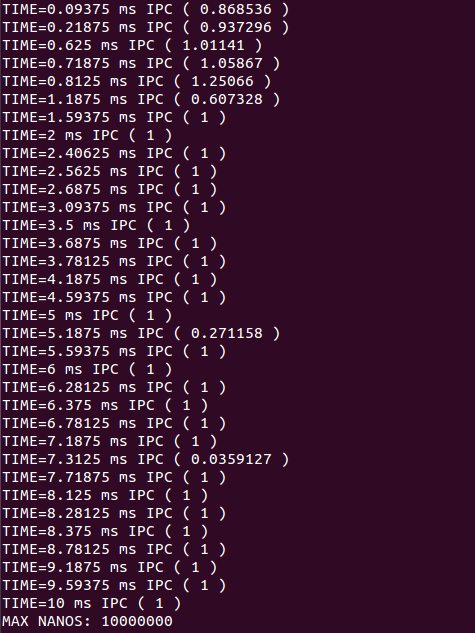
\includegraphics[width=3.2319in,height=4.3335in]{img36.png}
\par}

{\centering\selectlanguage{english}\sffamily\bfseries
\label{bkm:Ref388170618}Fig.
\stepcounter{Figure}{\theFigure} -- Expected output for dynamic sampler
example. The example is based on the dynamic.in Lua configuration file.
\par}

\subsubsection[Detailed instructions to start for Interval
Sampling]{\textrm{Detailed instructions to
start}\foreignlanguage{english}{\textrm{ for Interval Sampling}}}
{\selectlanguage{english}
\ To run the example, move on the example folder and then run the
example as follows:}

\begin{flushleft}
\tablehead{}
\begin{supertabular}{|m{6.21846in}|}
\hline
{\selectlanguage{english}\ttfamily \$ cd src/examples}

\selectlanguage{english} \texttt{\$ make
run\_multiple\_cpu\_interval}\\\hline
\end{supertabular}
\end{flushleft}
\subsubsection[Expected output for Interval Sampling]{\textrm{Expected
output}\foreignlanguage{english}{\textrm{ for Interval Sampling}}}
{\selectlanguage{english}
After launching the application the following output should be obtained
(see Fig. 21). As a variant, in this case 4 CPUs are simulated, the
simulation is fast-forwarded for 2 second and then the next 50 ms are
simulated with full timing but up to 5 samples that are taken at
successive regular instants:}

{\centering 
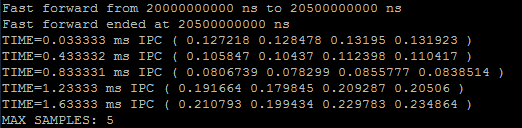
\includegraphics[width=4.5346in,height=1.1075in]{img37.png}
\par}

{\centering\selectlanguage{english}\sffamily\bfseries
\label{bkm:Ref388204406}Fig.
\stepcounter{Figure}{\theFigure} -- Expected output for interval based
sampler example. The example is based on the multiple\_cpu\_interval.in
Lua configuration file.
\par}

\subsubsection[Detailed instructions to start for SMARTS
Sampling]{\textrm{Detailed instructions to
start}\foreignlanguage{english}{\textrm{ for SMARTS Sampling}}}
{\selectlanguage{english}
\ To run the example, move on the example folder and then run the
example as follows:}

\begin{flushleft}
\tablehead{}
\begin{supertabular}{|m{6.21846in}|}
\hline
{\selectlanguage{english}\ttfamily \$ cd src/examples}

\selectlanguage{english} \texttt{\$ make run\_smarts}\\\hline
\end{supertabular}
\end{flushleft}
\subsubsection[Expected output for SMARTS Sampling]{\textrm{Expected
output}\foreignlanguage{english}{\textrm{ for SMARTS Sampling}}}
{\selectlanguage{english}
After launching the application the following output should be obtained
(see Fig. 21). In this case, similarly to the dynamic sampling, the
sampling instant are not uniformly distributed with the time:}

{\centering 
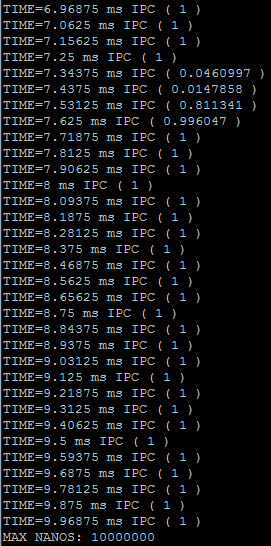
\includegraphics[width=2.0917in,height=4.2138in]{img38.png}
\par}

{\centering\selectlanguage{english}\sffamily\bfseries
Fig.
\stepcounter{Figure}{\theFigure} -- Expected output for SMARTS sampler
example. The example is based on the smarts.in Lua configuration file.
\par}

\subsection[Simulation of Ethernet connected
clusters]{\foreignlanguage{english}{Simulation of Ethernet connected
c}lusters}
{\selectlanguage{english}
A cluster is a set of loosely coupled computers that work together as if
they were a single computer. COTSon has the capability of simulating
clusters that are interconnected through an Ethernet based network card
and through a simulated switch (called
{\textquotedblleft}mediator{\textquotedblright}) by using an individual
full-system instance of SimNow for each node. It is worth of notice
that the SimNow instance run in parallel if the simulation host has
enough cores.}

\subsubsection[Goal of the experiment or example]{\rmfamily Goal of the
experiment or example}
{\selectlanguage{english}
When simulating a cluster with COTSon there is a software component that
is needed to connect all the SimNow instances of the different COTSon
nodes, called \textit{Mediator }(i.e., a component in the simulator
architecture that is responsible to manage the network communication
among different nodes of the simulated system -- see also Fig. 4). This
application, together with other external tools such as \textit{Slirp},
allows more than one COTSon node (i.e., an instance of SimNow plus
abaeterno) to communicate with the rest of the network. COTSon is
responsible for coordinating the activity of the nodes, which are
possibly running in different machines. The simplest example about
clusters is \textbf{\textit{twonodes.in}} that implements a cluster of
two nodes pinging each other.}

\subsubsection[Location of the involved files]{\rmfamily Location of the
involved files}
{\selectlanguage{english}
All the files needed to run the example are contained in the following
folder:}

\begin{flushleft}
\tablehead{}
\begin{supertabular}{|m{6.21846in}|}
\hline
\selectlanguage{english}
\texttt{\$COTSONHOME}\foreignlanguage{english}{\texttt{/src/examples}}\\\hline
\end{supertabular}
\end{flushleft}
{\selectlanguage{english}
Where \$\textbf{COTSONHOME }is an environment variable identifying the
installation path of the COTSon simulator.}

\subsubsection[Detailed instructions to start]{\rmfamily Detailed
instructions to start}
{\selectlanguage{english}
\ To run the example, move on the example folder and then run the
example as follows:}

\begin{flushleft}
\tablehead{}
\begin{supertabular}{|m{6.21846in}|}
\hline
{\selectlanguage{english}\ttfamily \$ cd src/examples}

\selectlanguage{english}\ttfamily \$ make run\_twonodes\\\hline
\end{supertabular}
\end{flushleft}
\subsubsection[Expected output]{\rmfamily Expected output}
{\selectlanguage{english}
After launching the application the following output should be obtained
(see Fig. 23):}

{\centering 
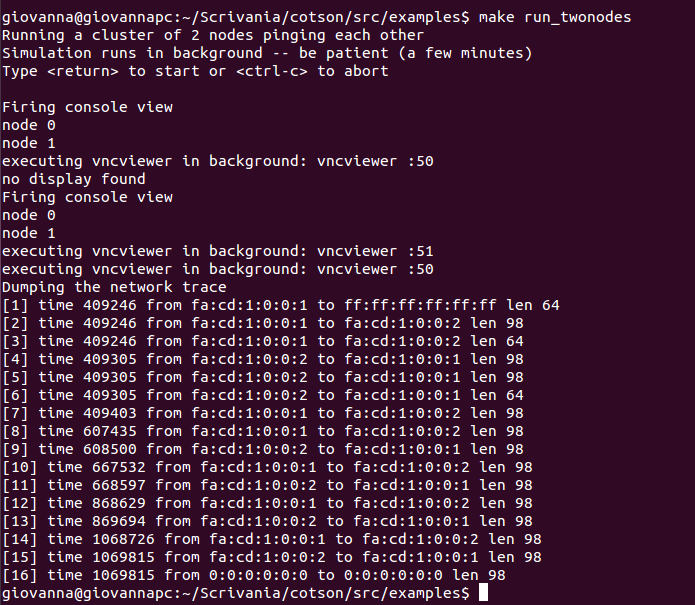
\includegraphics[width=4.8071in,height=3.5917in]{img39.png}
\par}

{\centering\selectlanguage{english}\sffamily\bfseries
\label{bkm:Ref388170779}Fig.
\stepcounter{Figure}{\theFigure} expected output for the example where
mediator component is used. The example is based on the twonodes.in Lua
configuration file.
\par}

{\selectlanguage{english}
While the simulation is running, the following windows (see Fig. 24)
should appear on the screen indicating that the two nodes have been
booted up and they are communicating each other:}

{\centering 
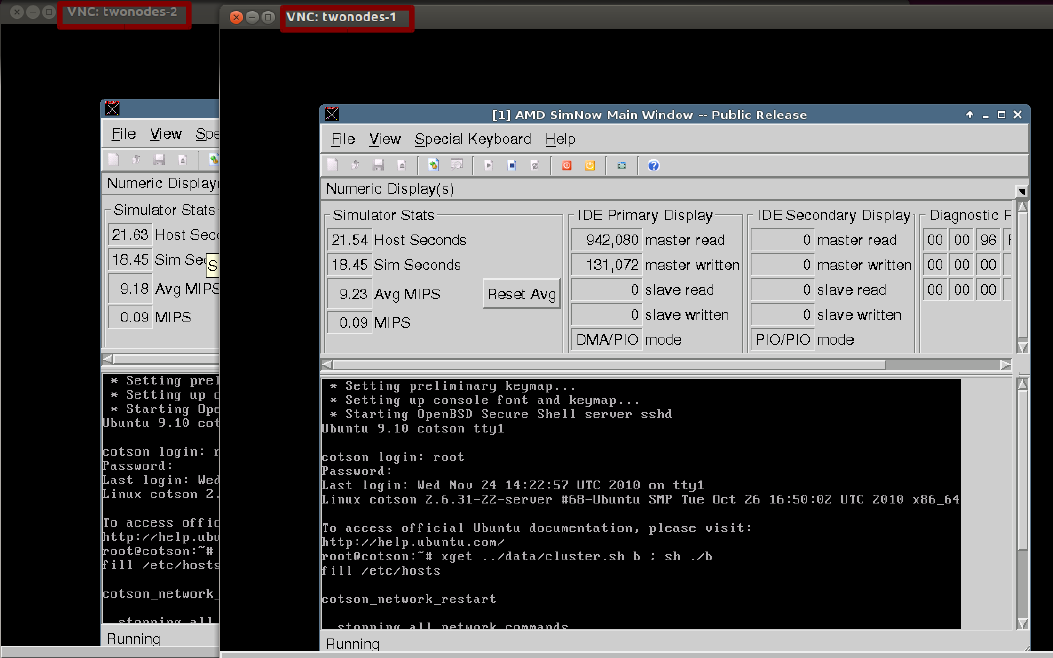
\includegraphics[width=5.1445in,height=3.2055in]{img40.png}
\par}

{\centering\selectlanguage{english}\sffamily\bfseries
\label{bkm:Ref388205414}Fig.
\stepcounter{Figure}{\theFigure}{}-- Two simulator windows are used to
manage the two communicating nodes of the simulated system.
\par}

\section[Research Use Case from BSC]{Research Use Case from BSC}
\label{bkm:Ref388218396}{\selectlanguage{english}
This section shows how to use the TERAFLUX system image and benchmark
repository that has been put in place to ensure partners use a common
development platform and can reproduce each other{\textquotesingle}s
results.}

\subsection[\ Goal of the experiment or example]{\ Goal of the
experiment or example}
{\selectlanguage{english}
The goal is two-fold: to show how the system image can be used for
development, and show how experiments from the benchmark repository can
be run.}

\subsection[Location of the involved files]{Location of the involved
files}
{\selectlanguage{english}
First of all, one must download the system image and verify its
integrity by downloading files}

\begin{flushleft}
\tablehead{}
\begin{supertabular}{|m{6.22196in}|}
\hline
\selectlanguage{english}\ttfamily wget
http://www.teraflux.eu/sites/teraflux.eu/files/teraflux-v5.img.bz2\\\hline
\end{supertabular}
\end{flushleft}
{\selectlanguage{english}
Then:}

\begin{flushleft}
\tablehead{}
\begin{supertabular}{|m{6.22196in}|}
\hline
\selectlanguage{english} \texttt{wget
http://www.teraflux.eu/sites/teraflux.eu/files/teraflux-v5.img.bz2.md5}\\\hline
\end{supertabular}
\end{flushleft}
{\selectlanguage{english}
Then executing:}

\begin{flushleft}
\tablehead{}
\begin{supertabular}{|m{6.22196in}|}
\hline
{\selectlanguage{english}\ttfamily \$ md5sum -c teraflux-v5.img.bz2.md5}

{\selectlanguage{english}\ttfamily teraflux-v5.img.bz2: OK}

\selectlanguage{english} \texttt{\$ bzip2 -d
teraflux-v5.img.bz2}\\\hline
\end{supertabular}
\end{flushleft}
{\selectlanguage{english}
Next, one must download the \textit{Teraflux Simulation Manager}
(\textit{tfsm}), a simple script to help using the image:}

\begin{flushleft}
\tablehead{}
\begin{supertabular}{|m{6.22196in}|}
\hline
\selectlanguage{english} \texttt{\$ svn co
}\texttt{https://teraflux.eu/svn/tfx/tfsm}\\\hline
\end{supertabular}
\end{flushleft}
{\selectlanguage{english}
This script requires installing a few packages, as well as support for
hardware virtualization in order to provide maximum performance during
development and native testing:}

\begin{flushleft}
\tablehead{}
\begin{supertabular}{|m{6.22196in}|}
\hline
{\selectlanguage{english} \texttt{\$ sudo apt-get --y install qemu-kvm
libvirt-bin vinagre qemu-system virt-manager gcc-4.4}}

{\selectlanguage{english}\ttfamily {\dots}}

{\selectlanguage{english}\ttfamily \$ sudo adduser
{\textasciigrave}whoami{\textasciigrave} kvm}

{\selectlanguage{english}\ttfamily \$ sudo addgroup libvirt}

{\selectlanguage{english}\ttfamily \$ sudo adduser
{\textasciigrave}whoami{\textasciigrave} libvirt}

\selectlanguage{english}\ttfamily \$ sudo modprobe kvm-amd\\\hline
\end{supertabular}
\end{flushleft}
{\selectlanguage{english}
The benchmark repository is included in the image file, but it can also
be independently downloaded:}

\begin{flushleft}
\tablehead{}
\begin{supertabular}{|m{6.22196in}|}
\hline
\selectlanguage{english} \texttt{\$ svn co
}\texttt{https://teraflux.eu/svn/tfx/ems}\\\hline
\end{supertabular}
\end{flushleft}
\subsection[Detailed instructions to start]{Detailed instructions to
start}
{\selectlanguage{english}
\ To start developing with the image, one must start \textit{tfsm} with
the following command:}

\begin{flushleft}
\tablehead{}
\begin{supertabular}{|m{6.22196in}|}
\hline
\selectlanguage{english}\ttfamily \$ ./tfsm/tfsm edit teraflux-v5.img
512 2\\\hline
\end{supertabular}
\end{flushleft}
{\selectlanguage{english}
This will start a virtual machine with 2 cores and 512 MB of memory,
ready to use for development and benchmark testing. Once the virtual
machine is running, one can start installing programs and developing.
Both the login and password are \textit{user}.}

{\selectlanguage{english}
After the changes are ready, one can launch multiple nodes to test the
benchmarks natively. First of all, the maximum number of nodes must be
established (2 in this case), and the editable virtual machine must be
stopped. The following commands have to be issued at the virtual
machine prompt:}

\begin{flushleft}
\tablehead{}
\begin{supertabular}{|m{6.22196in}|}
\hline
{\selectlanguage{english}\ttfamily \$ sudo ./guest/nodes 2}

\selectlanguage{english}\ttfamily \$ sudo halt\\\hline
\end{supertabular}
\end{flushleft}
{\selectlanguage{english}
One can then start two identical nodes to run distributed benchmarks
natively with \textit{tfsm}:}

\begin{flushleft}
\tablehead{}
\begin{supertabular}{|m{6.22196in}|}
\hline
{\selectlanguage{english}\ttfamily \$ ./tfsm/tfsm qemu teraflux-v5.img 2
512 2}

{\selectlanguage{english}\ttfamily Creating inter-node network...}

{\selectlanguage{english}\ttfamily Creating VMs...}

{\selectlanguage{english} \texttt{You can now connect to the VMs (e.g.,
{\textquotesingle}virt-manager{\textquotesingle} or
{\textquotesingle}vinagre :5900{\textquotesingle})}}

\selectlanguage{english}\ttfamily [Press enter to destroy all
Vms]\\\hline
\end{supertabular}
\end{flushleft}
{\selectlanguage{english}
The benchmarks are run with the \textit{Experiment Management System}
(\textit{ems}) that is included in the image (this command again can be
issued inside the virtual machine):}

\begin{flushleft}
\tablehead{}
\begin{supertabular}{|m{6.22196in}|}
\hline
{\selectlanguage{english}\ttfamily \$ cd ems}

\selectlanguage{english}\ttfamily \$ ./ems run kernels/cholesky
small\\\hline
\end{supertabular}
\end{flushleft}
\subsection[Expected output]{Expected output}
\begin{flushleft}
\tablehead{}
\begin{supertabular}{|m{6.22196in}|}
\hline
{\selectlanguage{english}\ttfamily Running
{\textquotesingle}kernels/cholesky/smpss{\textquotesingle} small into
kernels/cholesky/smpss//run/1}

{\selectlanguage{english}\ttfamily \$ cat
kernels/cholesky/smpss/run/1/ems\_output}

{\selectlanguage{english}\ttfamily + cholesky\_simple 64 64}

\selectlanguage{english}\ttfamily 25003147; \ \ \ \ \ \ 907\\\hline
\end{supertabular}
\end{flushleft}
{\selectlanguage{english}
Since the experiment is natively run in
{\textquotedblleft}\textit{qemu}{\textquotedblright} mode (using
hardware virtualization), the actual contents of the
\textit{ems\_output} file will change.}

\subsection[Further references to more in{}-depths]{Further references
to more in-depths}
{\selectlanguage{english}
The \textit{tfsm} script also includes commands to start SimNOW and
COTSon nodes. Please refer to the README file in the \textit{tfsm}
repository, and the environment-specific details of other partners for
more information on the necessary arguments.}

{\selectlanguage{english}
The \textit{ems} script also handles benchmark compilation, even though
the TERAFLUX disk image comes with pre-compiled benchmarks. Please run
\textit{ems} without arguments and read the \textit{README} file in the
\textit{ems} repository for more details. To update the benchmark
repository in the TERAFLUX disk image run:}

\begin{flushleft}
\tablehead{}
\begin{supertabular}{|m{6.22196in}|}
\hline
{\selectlanguage{english}\ttfamily \$ cd ems}

\selectlanguage{english} \texttt{\$ svn
}\texttt{https://teraflux.eu/svn/tfx/ems}
\texttt{update}\\\hline
\end{supertabular}
\end{flushleft}

\bigskip

\section[Research Use Case from CAPS]{Research Use Case from CAPS}
{\selectlanguage{english}
This section describe the experimental platform used to evaluate, first,
the new CAPS compiler back-end developed during the project, and second
the OpenACC dataflow extension, on the common TERAFLUX architecture
using the SimNOW virtualization system and the COTSon simulation
platform. The experimentation has been performed on a Convolution
benchmark programmed in OpenHMPP and offloading the parallel
computation on the CPU using a C back-end.}

\subsection[Goal of the experiment or example]{Goal of the experiment or
example}
{\selectlanguage{english}
The goal of the experiment is to validate the execution of the OpenHMPP
Convolution benchmark on the COTSon system. This experiment will
perform a functional validation of a code pre-compiled by the CAPS
compiler by the execution of the binary together with the CAPS compiler
runtime.}

\subsection[Location of the involved files]{Location of the involved
files}
{\selectlanguage{english}
To run the experiment, one has to use the tools implemented by the
collaborative effort from UNISI \& BSC: the COTSon simulation platform
with the associated SimNow virtualization system, and the
\textit{Teraflux Simulation Manager} (\textit{tfsm}). The COTSon system
is taken from the trunk:}

\begin{flushleft}
\tablehead{}
\begin{supertabular}{|m{6.15046in}|}
\hline
\selectlanguage{english}\ttfamily \$ svn co
https://svn.code.sf.net/p/cotson/code/trunk cotson\\\hline
\end{supertabular}
\end{flushleft}
{\selectlanguage{english}
The tfsm is fetched from the original source:}

\begin{flushleft}
\tablehead{}
\begin{supertabular}{|m{6.15046in}|}
\hline
\selectlanguage{english} \texttt{\$ svn co
}{\texttt{{https://teraflux.eu/svn/tfx/tfsm}}}\\\hline
\end{supertabular}
\end{flushleft}
{\selectlanguage{english}
The other files have been developed at CAPS entreprise using a branch of
the CAPS many-core compiler and the access is subject to a formal
request to CAPS entreprise:}

\begin{itemize}
\item {\selectlanguage{english}
\textit{karmic64-capse.img}: the image containing the CAPS compilation
framework and the Convolution example, it contains pre-compiled files
from the CAPS compiler, and requires only a minimal SDK;}
\item {\selectlanguage{english}
\textit{CAPSCompilersRuntimes-3.3.4-TF.tar.bz2}: the CAPS compiler
run-times for compiling the OpenHMPP applications;}
\item {\selectlanguage{english}
\textit{CAPSCompilersSDK-3.3.4-TF.tar.bz2}: the CAPS compiler SDK
(partial, without the compiler binaries, does not need a license token
generator);}
\item {\selectlanguage{english}
\textit{CAPSCompilersRuntimes-install.sh}: the automatic deployment
script;}
\item {\selectlanguage{english}
\textit{capse.in}: the Lua configuration script running the experiment
with timing enabled;}
\item {\selectlanguage{english}
\textit{capse-interactive.in}: the Lua configuration script running the
functional simulator in interactive mode;}
\end{itemize}
\subsection[Detailed instructions to start]{Detailed instructions to
start}
{\selectlanguage{english}\bfseries
Deployment}

{\selectlanguage{english}
This experiment requires the deployment of the CAPS-compiler run-time,
and the recompilation of the Convolution application on a virtual
machine image. For that purpose one has to use the
{\textquotedblleft}edit{\textquotedblright} mode of the \textit{tfsm}
(see previous section):}

\begin{flushleft}
\tablehead{}
\begin{supertabular}{|m{6.15046in}|}
\hline
\selectlanguage{english} \texttt{\$ ./tfsm edit karmic64-capse.img 512
2}\\\hline
\end{supertabular}
\end{flushleft}
{\selectlanguage{english}
Then, one has to perform a standard installation of the prototype
CAPS-compiler run-time and simply builds the Convolution application.
Note that these operations are easier to perform when \textit{tfsm} is
modified to run QEMU with a tunnel for SSH in port 2222:}

\begin{flushleft}
\tablehead{}
\begin{supertabular}{|m{6.15046in}|}
\hline
{\selectlanguage{english}\ttfamily \$ cp tfsm tfsm-capse}

{\selectlanguage{english}\ttfamily {\textless}REPLACE the corresponding
lines below in tfsm-capse{\textgreater}}

{\selectlanguage{english}\ttfamily cmd\_edit () \{}

{\selectlanguage{english} \ \ \ \ \texttt{which \$QEMU
{\textgreater}/dev/null {\textbar}{\textbar} error
{\textquotedbl}cannot find QEMU: \$QEMU{\textquotedbl}}}

{\selectlanguage{english} \ \ \ \ \texttt{sys \$QEMU -enable-kvm -hda
\$IMAGE -m \$MEM -smp \$NCORES -redir tcp:2222::22}}

\selectlanguage{english}\ttfamily \}\\\hline
\end{supertabular}
\end{flushleft}
{\selectlanguage{english}
Doing so, the update process can be automatize using \texttt{rsync} and
\texttt{ssh} commands from the host:}

\begin{flushleft}
\tablehead{}
\begin{supertabular}{|m{6.15046in}|}
\hline
{\selectlanguage{english} \texttt{\$ ./tfsm-capse edit
karmic64-capse.img 2048 8 \&}}

{\selectlanguage{english} \texttt{\$ scp -P 2222
CAPSCompilersRuntimes-install.sh root@localhost:/home/user/CAPSe/}}

{\selectlanguage{english} \texttt{\$ scp -P 2222
CAPSCompilersRuntimes-3.3.4-TF.tar.bz2
root@}\texttt{localhost}\texttt{:/home/user/CAPSe/}}

{\selectlanguage{english} \texttt{\$ scp -P 2222
CAPSCompilersSDK-3.3.4-TF.tar.bz2
root@}\texttt{localhost}\texttt{:/home/user/CAPSe/}}

{\selectlanguage{english} \texttt{\$ ssh -p 2222 root@localhos7
/home/user/CAPSe/CAPSCompilersRuntimes-install.sh}}

\selectlanguage{english} \texttt{\$ ssh -p 2222 root@localhost
{\textquotesingle}shutdown -h now{\textquotesingle}}\\\hline
\end{supertabular}
\end{flushleft}
{\selectlanguage{english}
On Ubuntu/Debian Linux distributions, the usage of the QEMU virtual
machine requires the user to belong to the
{\textquotedblleft}kvm{\textquotedblright} group (as in the previous
example of Section 7). Note that in this example, the host machine is
called {\textquotedblleft}localhost{\textquotedblright} and executes
the COTSon system. Once the deployment of the CAPS-compiler performed
on the COTSon system has been done, the experimental snapshot is
prepared using the SimNOW: }

\begin{flushleft}
\tablehead{}
\begin{supertabular}{|m{6.15046in}|}
\hline
{\selectlanguage{english}\ttfamily \$ export
PATH={\textquotedblright}\$PATH:.{\textquotedblright}; ln --s
../simnow-linux64-4.6.2pub/simnow}

\selectlanguage{english} \texttt{\$ }\texttt{./tfsm-capse simnow
karmic64-capse.img 4 4p-reset.bsd}\\\hline
\end{supertabular}
\end{flushleft}
{\selectlanguage{english}
Note also that the \textit{tfsm} script needs to know the installation
location of the SimNow virtualization system (it can be set through the
SIMNOW environmental variable). At the end of the boot process, the
snapshot is prepared with the appropriate environment (in the console
after the login root/root):}

\begin{flushleft}
\tablehead{}
\begin{supertabular}{|m{6.15046in}|}
\hline
{\selectlanguage{english}\ttfamily \$ cd /home/user/CAPSe}

{\selectlanguage{english}\ttfamily \$ source CAPSMC/bin/capsrt-env.sh}

{\selectlanguage{english}\ttfamily \$ cd Convolution}

\selectlanguage{english}\ttfamily \$ make clean \&\& make \\\hline
\end{supertabular}
\end{flushleft}
{\selectlanguage{english}
After the initialization is completed, the user should stop the
simulation and save the snapshot under the name
{\textquotedblleft}4p-capse.bsd{\textquotedblright} in the COTSon data
directory.}

{\selectlanguage{english}\bfseries
COTSon Simulation}

{\selectlanguage{english}
The functional validation is performed using a snapshot containing the
CAPS-compiler run-time and the Convolution example ready to run. A very
simple Lua configuration script (\textit{capse.in}) is called using the
following command:}

\begin{flushleft}
\tablehead{}
\begin{supertabular}{|m{6.15046in}|}
\hline
\selectlanguage{english} \texttt{\$ ../cotson/bin/cotson
capse.in}\foreignlanguage{english}{\texttt{ }}\\\hline
\end{supertabular}
\end{flushleft}
{\selectlanguage{english}
The lua configuration script activates the standard timing of the
simulation using the abaeterno library and the
{\textquotedblleft}build{\textquotedblright} function. It also uses the
{\textquotedblleft}fastforward{\textquotedblright} keyword to delay the
simulation up to the OpenHMPP kernel execution. The simulation can be
switched in visual mode if the appropriate line comments are removed
from the Lua configuration script. The core command of the script is
the following:}

\begin{flushleft}
\tablehead{}
\begin{supertabular}{|m{6.15046in}|}
\hline
{\selectlanguage{english}\ttfamily simnow.commands=function()}

{\selectlanguage{english}\ttfamily
\ \ \ use\_bsd({\textquotesingle}4p-capse.bsd{\textquotesingle})}

{\selectlanguage{english}\ttfamily
\ \ \ use\_hdd({\textquotesingle}karmic64-capse.img{\textquotesingle})}

{\selectlanguage{english}\ttfamily \ \ \ set\_journal()}

{\selectlanguage{english}
\texttt{\ \ }\texttt{send\_keyboard({\textquotesingle}./convol-hmpp.exe
-e 1 data/Michal-*.tif -o ./Michal.tif{\textquotesingle})}}

\selectlanguage{english}\ttfamily end\\\hline
\end{supertabular}
\end{flushleft}
{\selectlanguage{english}
The functional validation of the computation is done by the comparison
of the picture generated by the Convolution execution with a valid
reference. The timing result of the simulation is stored in the file
{\textquotedblleft}node.1.hmpp\_simple.log{\textquotedblright}.}

{\selectlanguage{english}
An interactive mode is available with the script
{\textquotedblleft}capse-interactive.in{\textquotedblright}, a variant
of the previous one activating the functional simulator with the SimNow
window enabled. The user has to run the simulator, and then it can
interact with the application. An overview of the simulator window is
given in Fig. 25.}

\subsection[Expected output]{Expected output}
{\selectlanguage{english}
The deployment and installation output is the following. It must contain
a correct compilation of the Convolution example and a proper
execution.}

\begin{flushleft}
\tablehead{}
\begin{tiny}
\begin{supertabular}{|m{6.15046in}|}
\hline
{\selectlanguage{english} \texttt{\textbf{[laorans@nova18 \~{}]\$ ssh -p
2222 root@localhost
/home/user/CAPSe/CAPSCompilersRuntimes-install.sh}}}

{\selectlanguage{english}
\texttt{\textbf{root@localhost{\textquotesingle}s password:}}}

{\selectlanguage{english}\ttfamily\bfseries Uncompress package}

{\selectlanguage{english}\ttfamily\bfseries {}-{}-{}-{}-{}-{}- Clean
Convolution -{}-{}-{}-{}-}

{\selectlanguage{english}\ttfamily\bfseries rm -rf
\ \ \ *convolution*\_c.hmg \ \ \ *convolution*\_c.hmg.o
\ \ \ \ \ \ *convolution*\_c.hmg.rc.o
\ \ \ *convolution*\_c.hmg.fatbin}

{\selectlanguage{english}\ttfamily\bfseries rm -rf}

{\selectlanguage{english}\ttfamily\bfseries rm -rf
src/pictureInterface.o src/mainutils.o src/filters5x5.hmpp.o
src/main-hmpp.hmpp.o convol-hmpp.exe src/filters5x5\_c.translated.o
src/main-hmpp\_c.translated.o}

{\selectlanguage{english}\ttfamily\bfseries rm -rf src/*.hmpp.o
src/*.translated.o}

{\selectlanguage{english}\ttfamily\bfseries rm -rf
properties\_tune\_*.psc}

{\selectlanguage{english}\ttfamily\bfseries rm -rf *\_out.tif out*.tif}

{\selectlanguage{english}\ttfamily\bfseries rm -rf core.*}

{\selectlanguage{english}\ttfamily\bfseries rm -rf *.translated.i
*.extracted.* *.halt.* *.hdpp.* *.inline.* *.preproc.* *.capstune.i}

{\selectlanguage{english}\ttfamily\bfseries rm -rf
*\_\_hmpp\_acc\_region\_\_*.o *\_\_hmpp\_acc\_region\_\_*.fatbin
*\_\_hmpp\_acc\_region\_\_*.hmf}

{\selectlanguage{english}\ttfamily\bfseries {}-{}-{}-{}-{}-{}- Build
Convolution -{}-{}-{}-{}-}

{\selectlanguage{english}\ttfamily\bfseries gcc -Wall -fopenmp
-DHMPP\_V3b -DHMPP\_OPTIM\_2 -DHMPP\_C -c -O3 -Isrc/ -o
src/pictureInterface.o src/pictureInterface.c}

{\selectlanguage{english}\ttfamily\bfseries gcc -Wall -fopenmp
-DHMPP\_V3b -DHMPP\_OPTIM\_2 -DHMPP\_C -c -O3 -Isrc/ -o src/mainutils.o
src/mainutils.c}

{\selectlanguage{english}\ttfamily\bfseries gcc -Wall -fopenmp
-DHMPP\_V3b -DHMPP\_OPTIM\_2 -DHMPP\_C -c -O3 -Isrc/ -o
src/filters5x5.hmpp.o src/filters5x5\_c.translated.i}

{\selectlanguage{english} \texttt{\textbf{src/filters5x5.c:48: warning:
[2592?]hmppsi\_lookup[2592?] defined but not used}}}

{\selectlanguage{english}\ttfamily\bfseries src/filters5x5.c:54:
warning: [2592?]hmppsi\_g\_convolution\_lookup[2592?] defined but not
used}

{\selectlanguage{english} \texttt{\textbf{gcc -Wall -fopenmp -DHMPP\_V3b
-DHMPP\_OPTIM\_2 -DHMPP\_C -c -O3 -Isrc/ -o src/main-hmpp.hmpp.o
src/main-hmpp\_c.translated.i}}}

{\selectlanguage{english}\ttfamily\bfseries src/main-hmpp.c: In function
[2592?]main[2592?]:}

{\selectlanguage{english}\ttfamily\bfseries src/main-hmpp.c:49: warning:
ignoring \#pragma hmpp}

{\selectlanguage{english}\ttfamily\bfseries src/main-hmpp.c:58: warning:
ignoring \#pragma hmpp}

{\selectlanguage{english}\ttfamily\bfseries src/main-hmpp.c:59: warning:
ignoring \#pragma hmpp}

{\selectlanguage{english}\ttfamily\bfseries src/main-hmpp.c:60: warning:
ignoring \#pragma hmpp}

{\selectlanguage{english} \texttt{\textbf{src/main-hmpp.c: At top
level:}}}

{\selectlanguage{english}\ttfamily\bfseries src/main-hmpp.c:108:
warning: [2592?]hmppsi\_lookup[2592?] defined but not used}

{\selectlanguage{english}\ttfamily\bfseries g++ -c
-I/home/user/CAPSe/CAPSMC//include
-I/home/user/CAPSe/CAPSMC//include/openacc \ {}-fPIC -o
convolution\_c.hmg.o convolution\_c.hmg.cc}

{\selectlanguage{english} \texttt{\textbf{g++ -shared \ {}-fPIC -o
convolution\_c.hmg convolution\_c.hmg.o}}}

{\selectlanguage{english}\ttfamily\bfseries gcc -Wall -fopenmp
-DHMPP\_V3b -DHMPP\_OPTIM\_2 -DHMPP\_C -O3 -o convol-hmpp.exe
src/pictureInterface.o src/mainutils.o src/filters5x5.hmpp.o
src/main-hmpp.hmpp.o convolution\_c.hmg -lm -ltiff -lz
-Wl,-rpath,/home/user/CAPSe/CAPSMC//slib
-Wl,-rpath,/home/user/CAPSe/CAPSMC//lib -L/home/user/CAPSe/CAPSMC//lib
-lhmpprti -lhmpprt -lhmpperr -lhmppstr -lhmppos -lhmppabi -lhmppos
-lhmpplog -lphmpp -lhmpprl -lopenacci -lopenacc}

{\selectlanguage{english}\ttfamily\bfseries {}-{}-{}-{}-{}-{}- Run
Convolution -{}-{}-{}-{}-}

{\selectlanguage{english}\ttfamily\bfseries ./convol-hmpp.exe -e 1
data/Michal-Osmenda-Mont\_Saint\_Michel-CC\_BY\_SA\_2.0.tif -o
\ ./Michal-Osmenda-Mont\_Saint\_Michel-CC\_BY\_SA\_2.0\_out.tif}

{\selectlanguage{english}\ttfamily\bfseries [ \ \ \ \ 0.056758] ( 0)
WARN : Cannot find libOpenCL.so: dlopen() failed: libOpenCL.so: cannot
open shared object file: No such file or directory, disabling OPENCL
support.}

{\selectlanguage{english}\ttfamily\bfseries [ \ \ \ \ 0.058255] ( 0)
INFO : -{}-{\textgreater} allocate {\textless}convolution{\textgreater}
at src/main-hmpp.c:48}

{\selectlanguage{english}\ttfamily\bfseries [ \ \ \ \ 0.058295] ( 0)
INFO : \ \ \ \ \ \ \ \ \ \ \ \ \ \ {}- Acquire the device
{\textquotesingle}host\#0{\textquotesingle}}

{\selectlanguage{english}\ttfamily\bfseries [ \ \ \ \ 0.058362] ( 0)
INFO : \ \ \ \ \ \ {}- Allocate buffer
{\textquotesingle}filter5x5\_1::heigh{\textbar}filter5x5\_2::heigh{\textquotesingle}
(4 x [] = 4 bytes of host memory on device
{\textquotesingle}host\#0{\textquotesingle})}

{\selectlanguage{english}\ttfamily\bfseries [ \ \ \ \ 0.058408] ( 0)
INFO : \ \ \ \ \ \ {}- Allocate buffer
{\textquotesingle}filter5x5\_1::width{\textbar}filter5x5\_2::width{\textquotesingle}
(4 x [] = 4 bytes of host memory on device
{\textquotesingle}host\#0{\textquotesingle})}

{\selectlanguage{english}\ttfamily\bfseries [ \ \ \ \ 0.058440] ( 0)
INFO : \ \ \ \ \ \ {}- Allocate buffer
{\textquotesingle}filter5x5\_1::inRaster{\textbar}filter5x5\_2::outRaster{\textquotesingle}
(4 x [2793, 1920] = 21450240 bytes of host memory on device
{\textquotesingle}host\#0{\textquotesingle})}

{\selectlanguage{english}\ttfamily\bfseries [ \ \ \ \ 0.058473] ( 0)
INFO : \ \ \ \ \ \ {}- Allocate buffer
{\textquotesingle}filter5x5\_1::outRaster{\textbar}filter5x5\_2::inRaster{\textquotesingle}
(4 x [2793, 1920] = 21450240 bytes of host memory on device
{\textquotesingle}host\#0{\textquotesingle})}

{\selectlanguage{english}\ttfamily\bfseries [ \ \ \ \ 0.058505] ( 0)
INFO : {\textless}-{}- allocate {\textless}convolution{\textgreater} at
src/main-hmpp.c:48}

{\selectlanguage{english}\ttfamily\bfseries [ \ \ \ \ 0.058526] ( 0)
INFO : -{}-{\textgreater} allocate, data
{\textless}convolution{\textgreater} at src/main-hmpp.c:50}

{\selectlanguage{english}\ttfamily\bfseries [ \ \ \ \ 0.058551] ( 0)
INFO : \ \ \ \ \ \ \ \ {}- Allocate mirror 0x4040a0
{\textquotedbl}stencil1{\textquotedbl} (4 x [25] = 100 bytes of host
memory on device {\textquotesingle}host\#0{\textquotesingle})}

{\selectlanguage{english}\ttfamily\bfseries [ \ \ \ \ 0.058581] ( 0)
INFO : \ \ \ \ \ \ \ \ {}- Allocate mirror 0x404120
{\textquotedbl}stencil2{\textquotedbl} (4 x [25] = 100 bytes of host
memory on device {\textquotesingle}host\#0{\textquotesingle})}

{\selectlanguage{english}\ttfamily\bfseries [ \ \ \ \ 0.058610] ( 0)
INFO : {\textless}-{}- allocate, data
{\textless}convolution{\textgreater} at src/main-hmpp.c:50}

{\selectlanguage{english}\ttfamily\bfseries [ \ \ \ \ 0.058633] ( 0)
INFO : -{}-{\textgreater} advancedload, data
{\textless}convolution{\textgreater} at src/main-hmpp.c:54}

{\selectlanguage{english}\ttfamily\bfseries [ \ \ \ \ 0.058654] ( 0)
INFO : \ \ \ \ \ \ \ \ {}- Upload mirror 0x4040a0
{\textquotedbl}stencil1{\textquotedbl} (4 x [25] = 100 bytes to device
{\textquotesingle}host\#0{\textquotesingle})}

{\selectlanguage{english}\ttfamily\bfseries [ \ \ \ \ 0.058697] ( 0)
INFO : \ \ \ \ \ \ \ \ {}- Upload mirror 0x404120
{\textquotedbl}stencil2{\textquotedbl} (4 x [25] = 100 bytes to device
{\textquotesingle}host\#0{\textquotesingle})}

{\selectlanguage{english}\ttfamily\bfseries [ \ \ \ \ 0.058721] ( 0)
INFO : {\textless}-{}- advancedload, data
{\textless}convolution{\textgreater} at src/main-hmpp.c:54}

{\selectlanguage{english}\ttfamily\bfseries [ \ \ \ \ 0.058743] ( 0)
INFO : -{}-{\textgreater} advancedload, args
{\textless}convolution{\textgreater} at src/main-hmpp.c:57}

{\selectlanguage{english}\ttfamily\bfseries [ \ \ \ \ 0.058759] ( 0)
INFO : \ \ \ \ \ \ {}- Bind buffer
{\textquotesingle}filter5x5\_1::heigh{\textbar}filter5x5\_2::heigh{\textquotesingle}
to address 0x7fff69c4afd8 {\textquotesingle}opt.m\_expansion *
BYTES\_PER\_PIXEL * heigh{\textquotesingle}}

{\selectlanguage{english}\ttfamily\bfseries [ \ \ \ \ 0.058775] ( 0)
INFO : \ \ \ \ \ \ {}- Bind buffer
{\textquotesingle}filter5x5\_1::width{\textbar}filter5x5\_2::width{\textquotesingle}
to address 0x7fff69c4afd4 {\textquotesingle}width{\textquotesingle}}

{\selectlanguage{english}\ttfamily\bfseries [ \ \ \ \ 0.058790] ( 0)
INFO : \ \ \ \ \ \ {}- Bind buffer
{\textquotesingle}filter5x5\_1::inRaster{\textbar}filter5x5\_2::outRaster{\textquotesingle}
to address 0x2af3ac422010 {\textquotesingle}raster1{\textquotesingle}}

{\selectlanguage{english}\ttfamily\bfseries [ \ \ \ \ 0.058811] ( 0)
INFO : \ \ \ \ \ \ {}- Upload buffer
{\textquotesingle}filter5x5\_1::heigh{\textbar}filter5x5\_2::heigh{\textquotesingle}
(4 x [] = 4 bytes to device
{\textquotesingle}host\#0{\textquotesingle})}

{\selectlanguage{english}\ttfamily\bfseries [ \ \ \ \ 0.058835] ( 0)
INFO : \ \ \ \ \ \ {}- Upload buffer
{\textquotesingle}filter5x5\_1::width{\textbar}filter5x5\_2::width{\textquotesingle}
(4 x [] = 4 bytes to device
{\textquotesingle}host\#0{\textquotesingle})}

{\selectlanguage{english}\ttfamily\bfseries [ \ \ \ \ 0.058858] ( 0)
INFO : \ \ \ \ \ \ {}- Upload buffer
{\textquotesingle}filter5x5\_1::inRaster{\textbar}filter5x5\_2::outRaster{\textquotesingle}
(4 x [2793, 1920] = 21450240 bytes to device
{\textquotesingle}host\#0{\textquotesingle})}

{\selectlanguage{english}\ttfamily\bfseries [ \ \ \ \ 0.070573] ( 0)
INFO : {\textless}-{}- advancedload, args
{\textless}convolution{\textgreater} at src/main-hmpp.c:57}

{\selectlanguage{english}\ttfamily\bfseries [ \ \ \ \ 0.070656] ( 0)
INFO : -{}-{\textgreater} callsite {\textless}convolution{\textgreater}
at src/main-hmpp.c:62}

{\selectlanguage{english}\ttfamily\bfseries [ \ \ \ \ 0.070673] ( 0)
INFO : \ \ \ \ \ \ {}- Bind buffer
{\textquotesingle}filter5x5\_1::heigh{\textbar}filter5x5\_2::heigh{\textquotesingle}
to address 0x7fff69c4afd8 {\textquotesingle}opt.m\_expansion *
BYTES\_PER\_PIXEL * heigh{\textquotesingle}}

{\selectlanguage{english}\ttfamily\bfseries [ \ \ \ \ 0.070690] ( 0)
INFO : \ \ \ \ \ \ {}- Bind buffer
{\textquotesingle}filter5x5\_1::width{\textbar}filter5x5\_2::width{\textquotesingle}
to address 0x7fff69c4afdc {\textquotesingle}width{\textquotesingle}}

{\selectlanguage{english}\ttfamily\bfseries [ \ \ \ \ 0.070705] ( 0)
INFO : \ \ \ \ \ \ {}- Bind buffer
{\textquotesingle}filter5x5\_1::filter{\textquotesingle} to address
0x4040a0 {\textquotesingle}stencil1{\textquotesingle}}

{\selectlanguage{english}\ttfamily\bfseries [ \ \ \ \ 0.070720] ( 0)
INFO : \ \ \ \ \ \ {}- Bind buffer
{\textquotesingle}filter5x5\_1::inRaster{\textbar}filter5x5\_2::outRaster{\textquotesingle}
to address 0x2af3ac422010 {\textquotesingle}(Raster2D\_C )
raster1{\textquotesingle}}

{\selectlanguage{english}\ttfamily\bfseries [ \ \ \ \ 0.070735] ( 0)
INFO : \ \ \ \ \ \ {}- Bind buffer
{\textquotesingle}filter5x5\_1::outRaster{\textbar}filter5x5\_2::inRaster{\textquotesingle}
to address 0x2af3ad897010 {\textquotesingle}(Raster2D )
raster2{\textquotesingle}}

{\selectlanguage{english}\ttfamily\bfseries [ \ \ \ \ 0.070759] ( 0)
INFO : \ \ \ \ \ \ {}- Call codelet
{\textquotesingle}filter5x5\_1{\textquotesingle} (on device
{\textquotesingle}host\#0{\textquotesingle})}

{\selectlanguage{english}\ttfamily\bfseries [ \ \ \ \ 0.401762] ( 0)
INFO : {\textless}-{}- callsite {\textless}convolution{\textgreater} at
src/main-hmpp.c:62}

{\selectlanguage{english}\ttfamily\bfseries [ \ \ \ \ 0.401860] ( 0)
INFO : -{}-{\textgreater} callsite {\textless}convolution{\textgreater}
at src/main-hmpp.c:65}

{\selectlanguage{english}\ttfamily\bfseries [ \ \ \ \ 0.401878] ( 0)
INFO : \ \ \ \ \ \ {}- Bind buffer
{\textquotesingle}filter5x5\_1::heigh{\textbar}filter5x5\_2::heigh{\textquotesingle}
to address 0x7fff69c4afd8 {\textquotesingle}opt.m\_expansion *
BYTES\_PER\_PIXEL * heigh{\textquotesingle}}

{\selectlanguage{english}\ttfamily\bfseries [ \ \ \ \ 0.401895] ( 0)
INFO : \ \ \ \ \ \ {}- Bind buffer
{\textquotesingle}filter5x5\_1::width{\textbar}filter5x5\_2::width{\textquotesingle}
to address 0x7fff69c4afd4 {\textquotesingle}width{\textquotesingle}}

{\selectlanguage{english}\ttfamily\bfseries [ \ \ \ \ 0.401911] ( 0)
INFO : \ \ \ \ \ \ {}- Bind buffer
{\textquotesingle}filter5x5\_2::filter{\textquotesingle} to address
0x404120 {\textquotesingle}stencil2{\textquotesingle}}

{\selectlanguage{english}\ttfamily\bfseries [ \ \ \ \ 0.401926] ( 0)
INFO : \ \ \ \ \ \ {}- Bind buffer
{\textquotesingle}filter5x5\_1::outRaster{\textbar}filter5x5\_2::inRaster{\textquotesingle}
to address 0x2af3ad897010 {\textquotesingle}(Raster2D\_C )
raster2{\textquotesingle}}

{\selectlanguage{english}\ttfamily\bfseries [ \ \ \ \ 0.401941] ( 0)
INFO : \ \ \ \ \ \ {}- Bind buffer
{\textquotesingle}filter5x5\_1::inRaster{\textbar}filter5x5\_2::outRaster{\textquotesingle}
to address 0x2af3ac422010 {\textquotesingle}(Raster2D )
raster1{\textquotesingle}}

{\selectlanguage{english}\ttfamily\bfseries [ \ \ \ \ 0.401961] ( 0)
INFO : \ \ \ \ \ \ {}- Call codelet
{\textquotesingle}filter5x5\_2{\textquotesingle} (on device
{\textquotesingle}host\#0{\textquotesingle})}

{\selectlanguage{english}\ttfamily\bfseries [ \ \ \ \ 0.730020] ( 0)
INFO : {\textless}-{}- callsite {\textless}convolution{\textgreater} at
src/main-hmpp.c:65}

{\selectlanguage{english}\ttfamily\bfseries [ \ \ \ \ 0.730122] ( 0)
INFO : -{}-{\textgreater} delegatedstore, args
{\textless}convolution{\textgreater} at src/main-hmpp.c:68}

{\selectlanguage{english}\ttfamily\bfseries [ \ \ \ \ 0.730146] ( 0)
INFO : \ \ \ \ \ \ {}- Download buffer
{\textquotesingle}filter5x5\_1::inRaster{\textbar}filter5x5\_2::outRaster{\textquotesingle}
(4 x [2793, 1920] = 21450240 bytes from device
{\textquotesingle}host\#0{\textquotesingle})}

{\selectlanguage{english}\ttfamily\bfseries [ \ \ \ \ 0.735362] ( 0)
INFO : {\textless}-{}- delegatedstore, args
{\textless}convolution{\textgreater} at src/main-hmpp.c:68}

{\selectlanguage{english}\ttfamily\bfseries [ \ \ \ \ 0.839454] ( 0)
INFO : -{}-{\textgreater} free, data
{\textless}convolution{\textgreater} at src/main-hmpp.c:89}

{\selectlanguage{english}\ttfamily\bfseries [ \ \ \ \ 0.839540] ( 0)
INFO : \ \ \ \ \ \ \ \ {}- Free mirror 0x4040a0
{\textquotedbl}stencil1{\textquotedbl} (4 x [25] = 100 bytes on device
{\textquotesingle}host\#0{\textquotesingle})}

{\selectlanguage{english}\ttfamily\bfseries [ \ \ \ \ 0.839600] ( 0)
INFO : \ \ \ \ \ \ \ \ {}- Free mirror 0x404120
{\textquotedbl}stencil2{\textquotedbl} (4 x [25] = 100 bytes on device
{\textquotesingle}host\#0{\textquotesingle})}

{\selectlanguage{english}\ttfamily\bfseries [ \ \ \ \ 0.839626] ( 0)
INFO : {\textless}-{}- free, data {\textless}convolution{\textgreater}
at src/main-hmpp.c:89}

{\selectlanguage{english}\ttfamily\bfseries [ \ \ \ \ 0.839645] ( 0)
INFO : -{}-{\textgreater} release {\textless}convolution{\textgreater}
at src/main-hmpp.c:90}

{\selectlanguage{english}\ttfamily\bfseries [ \ \ \ \ 0.839663] ( 0)
INFO : \ \ \ \ \ \ \ \ {}- Free buffer
{\textquotesingle}filter5x5\_1::outRaster{\textbar}filter5x5\_2::inRaster{\textquotesingle}
(4 x [2793, 1920] = 21450240 bytes on device
{\textquotesingle}host\#0{\textquotesingle})}

{\selectlanguage{english}\ttfamily\bfseries [ \ \ \ \ 0.841287] ( 0)
INFO : \ \ \ \ \ \ \ \ {}- Free buffer
{\textquotesingle}filter5x5\_1::inRaster{\textbar}filter5x5\_2::outRaster{\textquotesingle}
(4 x [2793, 1920] = 21450240 bytes on device
{\textquotesingle}host\#0{\textquotesingle})}

{\selectlanguage{english}\ttfamily\bfseries [ \ \ \ \ 0.842541] ( 0)
INFO : \ \ \ \ \ \ \ \ {}- Free buffer
{\textquotesingle}filter5x5\_1::heigh{\textbar}filter5x5\_2::heigh{\textquotesingle}
(4 x [] = 4 bytes on device
{\textquotesingle}host\#0{\textquotesingle})}

{\selectlanguage{english}\ttfamily\bfseries [ \ \ \ \ 0.842586] ( 0)
INFO : \ \ \ \ \ \ \ \ {}- Free buffer
{\textquotesingle}filter5x5\_1::width{\textbar}filter5x5\_2::width{\textquotesingle}
(4 x [] = 4 bytes on device
{\textquotesingle}host\#0{\textquotesingle})}

{\selectlanguage{english}\ttfamily\bfseries [ \ \ \ \ 0.842627] ( 0)
INFO : \ \ \ \ \ \ \ \ \ \ {}- Release the device
{\textquotesingle}host\#0{\textquotesingle}}

{\selectlanguage{english}\ttfamily\bfseries [ \ \ \ \ 0.842655] ( 0)
INFO : {\textless}-{}- release {\textless}convolution{\textgreater} at
src/main-hmpp.c:90}

\selectlanguage{english} \texttt{\textbf{Kernel time:
0.676843}}\texttt{\textbf{ }}\\\hline
\end{supertabular}
\end{tiny}
\end{flushleft}
{\selectlanguage{english}
The correct result of the COTSon simulation in visual mode is showed in
Fig. 25. Please note that the warning message is normal, considering
that the platform does not support OpenCL.}

{\centering 
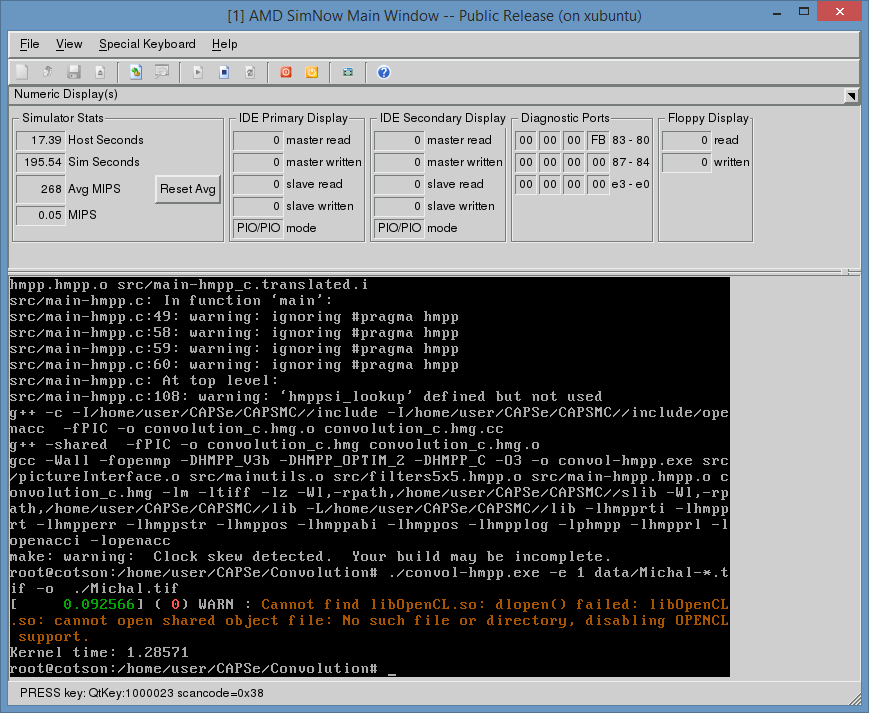
\includegraphics[width=3.9374in,height=3.2307in]{img41.png}
\par}

{\centering\selectlanguage{english}\sffamily\bfseries
\label{bkm:Ref388170667}Fig.
\stepcounter{Figure}{\theFigure} -- Results of a COTSon simulation on
the OpenHMPP Convolution example.
\par}

\subsection[Further references to more in{}-depths]{Further references
to more in-depths}
{\selectlanguage{english}
Further details about the CAPS many-core compiler can be found CAPS
ENTERPRISE web site.}


\bigskip

\section[Research Use Case from HP]{Research Use Case from HP}
{\selectlanguage{english}
This section describes the mapping of TERAFLUX applications, compiled to
T* ISA, and running on the simulation platform. This work was driven by
HP in collaboration with all partners.}

\subsection[Goal of the experiment or example]{Goal of the experiment or
example}
{\selectlanguage{english}
By performing simulations and analyzing the results with a full-system
simulator, one can gain a thorough understanding of how the proposed
architecture behaves, how to improve it, and how to validate the
results. The focus of this section is not the precise timing model in
simulation, but the capability to simulate interesting benchmarks on
thousands of cores, and multiple nodes, through the T* ISA. While the
current evaluation does not yet provide precise inter-node timing
results, the preliminary evaluation already enables scalability
measurements, addressing the dominant performance bottlenecks of the
applications.}

{\selectlanguage{english}
Another aspect of this section is the mitigation of resource
requirements in many-node simulation. Multiple nodes simulation of
parallel programs requires more resources than single node simulation.
Unless precautions are taken, programs with tremendous parallelism or
running on a large number of nodes will saturate memory resources, and
even deadlock, on any host machine. In the following the resource
requirements in the host and guest machine will be analyzed, and a set
of solutions to reduce the memory usage both in host machine and guest
machine will be also proposed. The solutions are implemented and
integrated in the COTSon simulator.}

\begin{center}
\begin{minipage}{6.2492in}
{\centering 
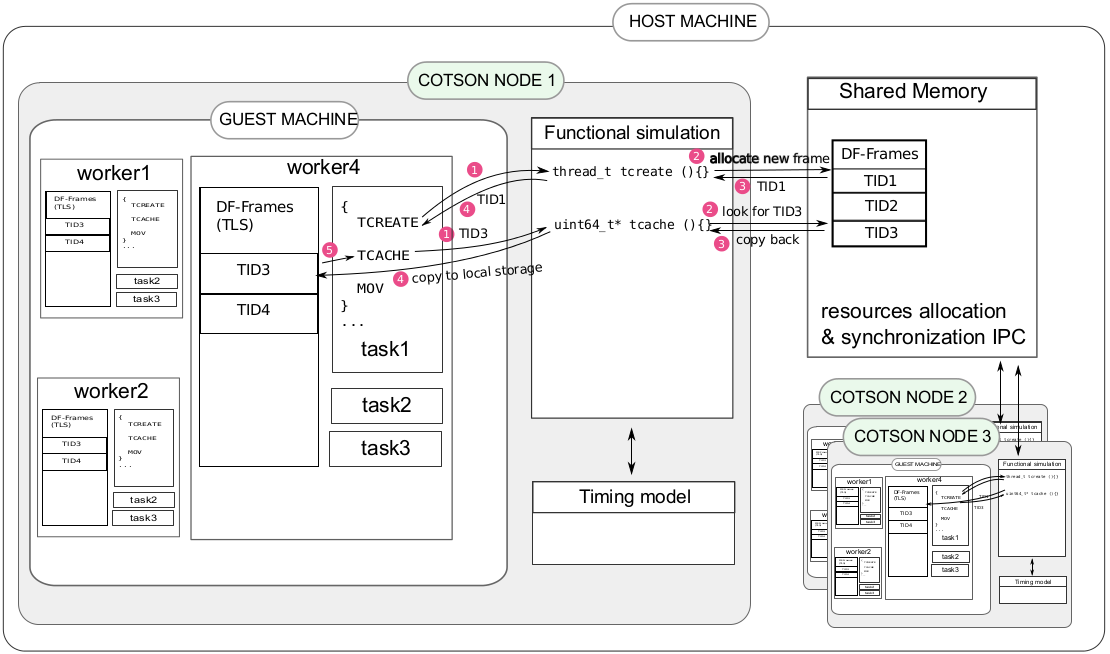
\includegraphics[width=6.2736in,height=3.6957in]{img42.png}
\par}

{\centering\selectlanguage{english}\sffamily\bfseries
\label{bkm:Ref388170757}Fig. \stepcounter{Figure}{\theFigure} --
Multi-node simulation with COTSon
\par}


\bigskip
\end{minipage}
\end{center}
{\selectlanguage{english}
Fig. 26 shows the multiple-nodes simulation structure on COTSon. The
host machine is where the COTSon instances are running on. COTSon
supports multiple-nodes simulation by allowing multiple instances of
COTSon, while the communication and synchronization of the instances go
through the mediator component. The \textit{guest} machine is the
machine (both hardware and operating system level) that is simulated by
a COTSon instance. One worker for each CPU within the guest machine is
created. Each worker will poll the centralized task queue for ready
tasks. At the execution of each task, the T* instructions will be
trapped by COTSon for functional simulation. In the figure, task 1 in
worker 4 (COTSon node 1), TCREATE (i.e., TSCHEDULE in [6]) and TCACHE
will be trapped by COTSon, and call the registered functions
\textit{tcreate} and \textit{tload} on the COTSon node where the guest
machine is simulated on, respectively. For the purpose of illustrating
how dataflow applications are managed within the simulation platform,
the T* instructions{\textquoteright} implementation in the COTSon
simulator is briefly recalled:}

\begin{itemize}
\item {\selectlanguage{english}
\textbf{\textit{TCREATE}} is trapped by COTSon to the functional
simulation, and then the registered function \textit{tcreate} will be
called (Fig. 23, step 1 and 2). It will try to allocate a new DF-frame
for the new DF-thread in the shared memory. If allocation is
successful, the new identifier for the DF-frame (TID1 in this case)
will be returned as the result of the execution of the assemble
TCREATE. DF-frames in shared memory is shared by all COTSon processes,
and protected with locks.}
\item {\selectlanguage{english}
\textbf{\textit{TCACHE}} is used to cache the remote frame locally. It
will be trapped by the functional simulation, and then the registered
function \textit{tcache} will be called. The DF-frame id is passed
along with TCACHE. In step 2, it will look up for TID3 in the shared
DF-Frames, if it is found, the entire DF-frame will be copied from host
to guest. More precisely, the DF-frame will be copied from the shared
memory to the local heap for this worker thread and the local
copy{\textquoteright}s pointer will be returned to TCACHE finally (step
5). Then in this task, one could directly modify/read this DF-frame. At
the time \textit{tdestroy} is called, the modifications will be
synchronized and could be seen by other tasks/nodes.}
\item {\selectlanguage{english}
\textbf{\textit{TLOAD}} is a shortcut for a specialized, current-thread
version of TCACHE. It will be trapped by the functional simulation, and
then the registered function \textit{tload} will be called. The current
thread id is stored within thread local storage and used to get current
DF-frame in the shared DF-Frames, if it is found, the DF-Frame will be
copied from host to guest, and the local copy{\textquoteright}s pointer
will be returned to TLOAD. Another difference between TLOAD and TCACHE
is that the frame loaded by TLOAD is read-only. The data stored in the
DF-frame is needed by the computations in the current thread.}
\item {\selectlanguage{english}
\textbf{\textit{TDECREASE}} makes the target thread designated by thread
id to be decremented by \textit{n} either at the time it is called
(eager tdecrease) or upon termination of the current thread (lazy
tdecrease, at the time TDESTORY is called). It will be trapped by the
functional simulation, and the registered function \textit{tdecrease}
will be called. In eager tdecrease, the target DF-frame id and is
passed along with TDECREASE. It will look up for the target DF-frame,
once it is found, it decreases the synchronization Count (SC) by
\textit{n}. Then it checks the value SC after decrement, if it reaches
to zero, the corresponding thread is moved to the ready queue. In lazy
tdecrease, the TDECREASE instruction will be cached.}
\item {\selectlanguage{english}
\textbf{\textit{TDESTROY}} is trapped to the functional simulation,
resulting in a call to the registered function \textit{tdestroy}. This
function will terminate the current thread and deallocate its DF-frame
in Shared DF-Frames. If running in lazy mode, it will aggregate and
execute the cached instructions (e.g. several TDECREASE to the same
thread will be aggregated to a single TDECREASE) before deallocation.}
\end{itemize}
{\selectlanguage{english}
Note that the implementation of the T* ISA extension in the COTSon
simulator covers the development of the distributed Thread Scheduling
Unit models (TSUF described in this section, and TSU4 described in
section 17).}

{\selectlanguage{english}
With the aim of investigating the performance of the T* instruction
implementation in the COTSon simulator, a set of experiments with
multiple-node simulations using 5 benchmarks (Fibonacci, Gauss Seidel,
Matrix Multiplication, Sparse LU and Viola Jones -
Thales{\textquotesingle}s pedestrian detection) have been conducted.
Except for Fibonacci, all benchmarks make use of the Owner Writable
Memory (OWM) support. The benchmarks have been implemented in two
different flavors. One flavor is to write programs with the low level
T* instruction set using C-level
{\textquotedblleft}built-in{\textquotedblright}s (Fibonacci and Matrix
Multiplication); the other flavor uses OpenStream and the TERAFLUX
compiler support to express dataflow parallelism, and has been used for
the more complex benchmarks (Gauss Seidel, Sparse LU and Viola Jones).
The multi-node implementation for the latter benchmarks uses the
OpenStream extension for OWM. The run-time support library for
OpenStream (to match dependences over streams) is integrated into the
COTSon run-time. }

\begin{itemize}
\item {\centering 
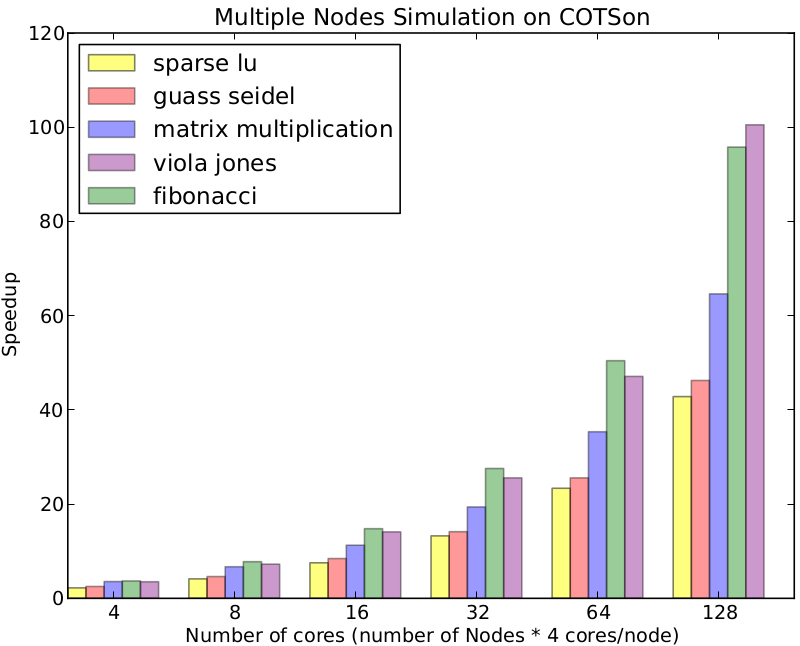
\includegraphics[width=3.3772in,height=2.7181in]{img43.png}
\par}
\end{itemize}
{\centering\selectlanguage{english}\sffamily\bfseries
\label{bkm:Ref388222100}Fig.
\stepcounter{Figure}{\theFigure} -- Speedup of five different dataflow
benchmarks running on different number of cores/nodes.
\par}

{\selectlanguage{english}
A few results on 128 cores and 32 nodes are shown in Fig. 27. More
details can be found in the WP2 deliverable. With the aim of enabling
the reader to run one of these specific benchmarking examples, in the
following the single node simulation of Matrix Multiplication benchmark
is described in details.}

\subsection[Location of the involved files]{Location of the involved
files}
{\selectlanguage{english}
All example files and instructions are provided on the TSUF branch of
COTSon (we assume here that the checkout of \$COTSON-ROOT involves not
only the trunk as in Sect. 1.1, but also the branches):}

\begin{flushleft}
\tablehead{}
\begin{supertabular}{|m{6.34626in}|}
\hline
\selectlanguage{english}\ttfamily
\$COTSON-ROOT/branches/tflux-test/tsuf\\\hline
\end{supertabular}
\end{flushleft}
{\selectlanguage{english}
The software stack uses the DF-proxies branch of the OpenStream
compiler, where we integrated our T* backend implementation and OWM
support. The simulated architecture uses SimNow version 4.6.2, and the
most recent version of COTSon with support for T* architecture (the
TSUF branch). }

\subsection[Detailed instructions to start]{Detailed instructions to
start}
{\selectlanguage{english}
The \textit{Matrix Multiply} kernel generates a moderate number of
dataflow threads (namely DF-Threads), but stress more the TERAFLUX
architecture from the computational viewpoint. In order to run the
example, move on the correct folder:}

\begin{flushleft}
\tablehead{}
\begin{supertabular}{|m{6.34626in}|}
\hline
\selectlanguage{english}\ttfamily \$ cd
\$COTSON-ROOT/branches/tflux-test/tsuf\\\hline
\end{supertabular}
\end{flushleft}
{\selectlanguage{english}
Open the \textit{Makefile} file with a text editor and check that the
first line is correctly pointing the main COTSon folder. Then, in the
same file set the variable \textit{TESTS} to \textit{matmul}, in order
to run the selected benchmark:}

\begin{flushleft}
\tablehead{}
\begin{supertabular}{|m{6.34626in}|}
\hline
\selectlanguage{english}\ttfamily \$ vi Makefile\\\hline
{\selectlanguage{english}\ttfamily COTSON\_ROOT=\$(shell bash -c
{\textquotesingle}cd ../../../trunk; pwd{\textquotesingle})}

{\selectlanguage{english}\ttfamily COTSON\_SRC=\$(COTSON\_ROOT)/src}

{\selectlanguage{english}\ttfamily TSUSIM=tflux\_tsu.so}

{\selectlanguage{english}\ttfamily TESTS = matmul}

\selectlanguage{english}\ttfamily ...\\\hline
\end{supertabular}
\end{flushleft}
{\selectlanguage{english}
At this point one needs to run the build process for the local folder.
This operation is necessary to build the shared object library
(\textit{tflux\_tsu.so}) that contains the code used to implement the
thread scheduling unit:}

\begin{flushleft}
\tablehead{}
\begin{supertabular}{|m{6.34626in}|}
\hline
\selectlanguage{english}\ttfamily \$ make\\\hline
\end{supertabular}
\end{flushleft}
{\selectlanguage{english}
The next step is to enter in the benchmark folder and modify the local
\textit{Makefile} file (through a text editor), setting up the proper
configuration of the simulated system (i.e., size of the input of the
benchmark, number of cores, etc.). In particular, set the variable
\textit{COTSON} to point the main simulation folder corresponding to
the position \textit{COTSON-ROOT/trunk}. Then, set the size of the
benchmark input modifying the value associated to the variable
\textit{SZ} (here the value is 35). The number of cores used by the
simulated system is expressed by the value of the \textit{NT} variable
(in this example we run on a single node with 4 cores).}

\begin{flushleft}
\tablehead{}
\begin{supertabular}{|m{6.34626in}|}
\hline
{\selectlanguage{english}\ttfamily all: \$(TESTS)}

{\selectlanguage{english}\ttfamily COTSON=\$(shell bash -c
{\textquotesingle}cd ../../../../trunk;
pwd{\textquotesingle})/bin/cotson}

{\selectlanguage{english}\ttfamily DFDIR= \$(shell bash -c
{\textquotesingle}cd ..; pwd{\textquotesingle})}

{\selectlanguage{english}\ttfamily DFRT=\$(DFDIR)/dflib.o}

{\selectlanguage{english}\ttfamily DFLIBS=-lpthread}

{\selectlanguage{english}\ttfamily TSUSIM=\$(DFDIR)/tflux\_tsu.so}

{\selectlanguage{english}\ttfamily PWD=\$(shell pwd)}

{\selectlanguage{english}\ttfamily RM=rm -rf}

{\selectlanguage{english}\ttfamily TSCRIPT=\$(PWD)/tsutest}

{\selectlanguage{english}\ttfamily WSDIR=./libworkstream\_df}

{\selectlanguage{english}\ttfamily WSOPTS=-g -O0 -ffast-math
-D\_GNU\_SOURCE -I . -fPIC -Wall -Wextra -lpthread}

{\selectlanguage{english}\ttfamily OWMSZ=32000000}

{\selectlanguage{english}\ttfamily SZ=35}

{\selectlanguage{english}\ttfamily NT=4}

{\selectlanguage{english}\ttfamily TESTS = matmul}

{\selectlanguage{english}\ttfamily HTMTESTS = tmtest\_htm}

\selectlanguage{english}\ttfamily ...\\\hline
\end{supertabular}
\end{flushleft}
{\selectlanguage{english}
With the next step the reader has to check the Lua configuration file.
Since a single node simulation is running, the reader needs to open the
\textit{tsu\_single.lua} file with a text editor, and comment the
\textit{display} variable so that the whole simulation output will be
displayed on the console and copied also on text file. The
\textit{use\_bsd()} function is set to \textit{4p.bsd} in order to
launch a 4-cores system with SimNow. Similarly, the \textit{sampler}
object is set to \textit{no\_timing}, in order to run a pure functional
simulation. To run a timing simulation, the user must change the value
of this object to \textit{simple}.}

\begin{flushleft}
\tablehead{}
\begin{tiny}
\begin{supertabular}{|m{6.34626in}|}
\hline
{\selectlanguage{english}\ttfamily
runid={\textquotedbl}tsu{\textquotedbl}}

{\selectlanguage{english}\ttfamily abaeterno\_so=TSUSIM}

~

{\selectlanguage{english}\ttfamily
wd=os.getenv({\textquotedbl}PWD{\textquotedbl})}

{\selectlanguage{english}\ttfamily tmpdir=wd}

{\selectlanguage{english}\ttfamily debug=true}

{\selectlanguage{english}\ttfamily {}-{}- clean\_sandbox=false}

{\selectlanguage{english}\ttfamily TSULAT=1}

~

{\selectlanguage{english}\ttfamily options = \{}

{\selectlanguage{english}\ttfamily
\ \ \ \ {}-{}-max\_nanos={\textquotesingle}3G{\textquotesingle},}

{\selectlanguage{english}\ttfamily
\ \ \ \ exit\_trigger={\textquotesingle}terminate{\textquotesingle},}

{\selectlanguage{english}
\texttt{\ \ \ \ }\texttt{sampler=\{type={\textquotedbl}no\_timing{\textquotedbl},
quantum={\textquotedbl}10M{\textquotedbl}\},}}

{\selectlanguage{english}\ttfamily \ \ \ \ {}-{}-
sampler=\{type={\textquotedbl}interval{\textquotedbl},functional={\textquotedbl}20M{\textquotedbl},warming={\textquotedbl}100k{\textquotedbl},simulation={\textquotedbl}100k{\textquotedbl}\},}

{\selectlanguage{english} \texttt{\ \ \ \ }\texttt{{}-{}-
sampler=\{type={\textquotedbl}simple{\textquotedbl},
quantum={\textquotedbl}3M{\textquotedbl}\},}}

{\selectlanguage{english}\ttfamily \ \ \ \ heartbeat=\{
type={\textquotedbl}file\_last{\textquotedbl},
logfile=runid..{\textquotedbl}.log{\textquotedbl} \},}

{\selectlanguage{english}\ttfamily \ \ \ \ {}-{}-
interleaver\_order={\textquotedbl}round\_robin{\textquotedbl},}

{\selectlanguage{english}\ttfamily \ \ \ \ custom\_asm=true,}

{\selectlanguage{english}\ttfamily \ \ \ \ time\_feedback=true,}

{\selectlanguage{english}\ttfamily
\ \ \ \ tsu\_ignore\_errors={\textquotedbl}true{\textquotedbl},}

{\selectlanguage{english}\ttfamily \ \ \ \ {}-{}-
tsu\_speculative\_threads=true,}

{\selectlanguage{english}\ttfamily
\ \ \ \ tsu\_statfile={\textquotedbl}/tmp/xx.dat{\textquotedbl},}

{\selectlanguage{english}\ttfamily \ \ \ \ {}-{}-
tsu\_destroy\_polls=true,}

{\selectlanguage{english}\ttfamily \ \ \ \ {}-{}-
tsu\_keep\_target\_frames={\textquotedbl}false{\textquotedbl},}

~

{\selectlanguage{english}\ttfamily \ \ \ \ tsu\_def\_lat=1*TSULAT,}

{\selectlanguage{english}\ttfamily \ \ \ \ tsu\_rd\_lat=20*TSULAT,}

{\selectlanguage{english}\ttfamily \ \ \ \ tsu\_wr\_lat=10*TSULAT,}

{\selectlanguage{english}\ttfamily \ \ \ \ tsu\_sub\_lat=100*TSULAT,}

{\selectlanguage{english}\ttfamily \ \ \ \ tsu\_sch\_lat=1000*TSULAT,}

{\selectlanguage{english}\ttfamily \}}

~

{\selectlanguage{english}\ttfamily
one\_node\_script={\textquotedbl}run\_interactive{\textquotedbl}}

{\selectlanguage{english}\ttfamily {}-{}-
display=os.getenv({\textquotedbl}DISPLAY{\textquotedbl})}

{\selectlanguage{english}\ttfamily
copy\_files\_prefix=runid..{\textquotedbl}.{\textquotedbl}}

{\selectlanguage{english}\ttfamily {}-{}- clean\_sandbox=false}

~

{\selectlanguage{english}\ttfamily simnow.commands=function()}

{\selectlanguage{english}\ttfamily \ \ \ \ {}-{}-
use\_bsd({\textquotesingle}8p.bsd{\textquotesingle})}

{\selectlanguage{english}\ttfamily \ \ \ \ {}-{}-
use\_bsd({\textquotesingle}16p.bsd{\textquotesingle})}

{\selectlanguage{english}\ttfamily \ \ \ \ {}-{}-
use\_bsd({\textquotesingle}32p.bsd{\textquotesingle})}

{\selectlanguage{english}
\texttt{\ \ \ \ }\texttt{use\_bsd({\textquotesingle}4p.bsd{\textquotesingle})}}

{\selectlanguage{english}\ttfamily
\ \ \ \ use\_hdd({\textquotesingle}karmic64.img{\textquotesingle})}

{\selectlanguage{english}\ttfamily \ \ \ \ set\_journal()}

{\selectlanguage{english}\ttfamily \ \ \ \ execute(SCRIPT)}

{\selectlanguage{english}\ttfamily end}

~

{\selectlanguage{english}\ttfamily function build()}

{\selectlanguage{english}\ttfamily \ \ \ \ i=0}

{\selectlanguage{english}\ttfamily \ \ \ \ while i {\textless} disks()
do}

{\selectlanguage{english}\ttfamily \ \ \ \ \ \ \ \ disk=get\_disk(i)}

{\selectlanguage{english}\ttfamily \ \ \ \ \ \ \ \ disk:timer\{
name={\textquotesingle}disk{\textquotesingle}..i,
type={\textquotedbl}simple\_disk{\textquotedbl}, \}}

{\selectlanguage{english}\ttfamily \ \ \ \ \ \ \ \ i=i+1}

{\selectlanguage{english}\ttfamily \ \ \ \ end}

{\selectlanguage{english}\ttfamily \ \ \ \ i=0}

{\selectlanguage{english}\ttfamily \ \ \ \ while i {\textless} nics()
do}

{\selectlanguage{english}\ttfamily \ \ \ \ \ \ \ \ nic=get\_nic(i)}

\selectlanguage{english}\ttfamily ...\\\hline
\end{supertabular}
\end{tiny}
\end{flushleft}
{\selectlanguage{english}
At this point is possible to launch the simulation as follows:}

\begin{flushleft}
\tablehead{}
\begin{supertabular}{|m{6.34626in}|}
\hline
\selectlanguage{english}\ttfamily \$ make run\_single\\\hline
\end{supertabular}
\end{flushleft}
\subsection[Expected output]{Expected output}
{\selectlanguage{english}
The following files are involved in the output process. The file
\textit{node.1.tsu.log }contains the statistics gathered by COTSon
during the simulation:}

\begin{flushleft}
\tablehead{}
\begin{tiny}
\begin{supertabular}{|m{6.34626in}|}
\hline
{\selectlanguage{english}\ttfamily Input values:}

~

{\selectlanguage{english}\ttfamily cpu0.bpred\_perfect
\ \ \ \ \ \ \ \ \ \ \ \ \ \ \ \ \ \ \ \ \ \ \ \ \ \ \ \ \ \ \ \ \ \ \ \ \ \ \ \ \ false}

{\selectlanguage{english}\ttfamily
cpu0.branch\_mispred\_penalty
\ \ \ \ \ \ \ \ \ \ \ \ \ \ \ \ \ \ \ \ \ \ \ \ \ \ \ \ \ \ \ \ 8}

{\selectlanguage{english}\ttfamily cpu0.commit\_cpi
\ \ \ \ \ \ \ \ \ \ \ \ \ \ \ \ \ \ \ \ \ \ \ \ \ \ \ \ \ \ \ \ \ \ \ \ \ \ \ \ \ \ \ \ 1.0}

{\selectlanguage{english}\ttfamily cpu0.dcache.fudge
\ \ \ \ \ \ \ \ \ \ \ \ \ \ \ \ \ \ \ \ \ \ \ \ \ \ \ \ \ \ \ \ \ \ \ \ \ \ \ \ \ \ 1.0}

{\selectlanguage{english}\ttfamily cpu0.icache.fudge
\ \ \ \ \ \ \ \ \ \ \ \ \ \ \ \ \ \ \ \ \ \ \ \ \ \ \ \ \ \ \ \ \ \ \ \ \ \ \ \ \ \ 1.0}

{\selectlanguage{english}\ttfamily cpu0.twolev.hlength
\ \ \ \ \ \ \ \ \ \ \ \ \ \ \ \ \ \ \ \ \ \ \ \ \ \ \ \ \ \ \ \ \ \ \ \ \ \ \ \ 14}

{\selectlanguage{english}\ttfamily cpu0.twolev.l1\_size
\ \ \ \ \ \ \ \ \ \ \ \ \ \ \ \ \ \ \ \ \ \ \ \ \ \ \ \ \ \ \ \ \ \ \ \ \ \ \ \ 1}

{\selectlanguage{english}\ttfamily cpu0.twolev.l2\_size
\ \ \ \ \ \ \ \ \ \ \ \ \ \ \ \ \ \ \ \ \ \ \ \ \ \ \ \ \ \ \ \ \ \ \ \ \ \ \ \ 16kB}

{\selectlanguage{english}\ttfamily cpu0.twolev.use\_xor
\ \ \ \ \ \ \ \ \ \ \ \ \ \ \ \ \ \ \ \ \ \ \ \ \ \ \ \ \ \ \ \ \ \ \ \ \ \ \ \ 1}

{\selectlanguage{english}\ttfamily cpu0.type
\ \ \ \ \ \ \ \ \ \ \ \ \ \ \ \ \ \ \ \ \ \ \ \ \ \ \ \ \ \ \ \ \ \ \ \ \ \ \ \ \ \ \ \ \ \ \ \ \ \ timer0}

{\selectlanguage{english}\ttfamily cpu1.bpred\_perfect
\ \ \ \ \ \ \ \ \ \ \ \ \ \ \ \ \ \ \ \ \ \ \ \ \ \ \ \ \ \ \ \ \ \ \ \ \ \ \ \ \ false}

{\selectlanguage{english}\ttfamily
cpu1.branch\_mispred\_penalty
\ \ \ \ \ \ \ \ \ \ \ \ \ \ \ \ \ \ \ \ \ \ \ \ \ \ \ \ \ \ \ \ 8}

{\selectlanguage{english}\ttfamily cpu1.commit\_cpi
\ \ \ \ \ \ \ \ \ \ \ \ \ \ \ \ \ \ \ \ \ \ \ \ \ \ \ \ \ \ \ \ \ \ \ \ \ \ \ \ \ \ \ \ 1.0}

{\selectlanguage{english}\ttfamily cpu1.dcache.fudge
\ \ \ \ \ \ \ \ \ \ \ \ \ \ \ \ \ \ \ \ \ \ \ \ \ \ \ \ \ \ \ \ \ \ \ \ \ \ \ \ \ \ 1.0}

{\selectlanguage{english}\ttfamily cpu1.icache.fudge
\ \ \ \ \ \ \ \ \ \ \ \ \ \ \ \ \ \ \ \ \ \ \ \ \ \ \ \ \ \ \ \ \ \ \ \ \ \ \ \ \ \ 1.0}

{\selectlanguage{english}\ttfamily cpu1.twolev.hlength
\ \ \ \ \ \ \ \ \ \ \ \ \ \ \ \ \ \ \ \ \ \ \ \ \ \ \ \ \ \ \ \ \ \ \ \ \ \ \ \ 14}

{\selectlanguage{english}\ttfamily cpu1.twolev.l1\_size
\ \ \ \ \ \ \ \ \ \ \ \ \ \ \ \ \ \ \ \ \ \ \ \ \ \ \ \ \ \ \ \ \ \ \ \ \ \ \ \ 1}

{\selectlanguage{english}\ttfamily cpu1.twolev.l2\_size
\ \ \ \ \ \ \ \ \ \ \ \ \ \ \ \ \ \ \ \ \ \ \ \ \ \ \ \ \ \ \ \ \ \ \ \ \ \ \ \ 16kB}

{\selectlanguage{english}\ttfamily ...}

{\selectlanguage{english}\ttfamily ...}

~

{\selectlanguage{english}\ttfamily Output values:}

~

{\selectlanguage{english}\ttfamily cpu0.cycles
\ \ \ \ \ \ \ \ \ \ \ \ \ \ \ \ \ \ \ \ \ \ \ \ \ \ \ \ \ \ \ \ \ \ \ \ \ \ \ \ \ \ \ \ \ \ \ \ 1309999869}

{\selectlanguage{english}\ttfamily cpu0.haltcount
\ \ \ \ \ \ \ \ \ \ \ \ \ \ \ \ \ \ \ \ \ \ \ \ \ \ \ \ \ \ \ \ \ \ \ \ \ \ \ \ \ \ \ \ \ 819583852}

{\selectlanguage{english}\ttfamily cpu0.hb\_ATC\_flush
\ \ \ \ \ \ \ \ \ \ \ \ \ \ \ \ \ \ \ \ \ \ \ \ \ \ \ \ \ \ \ \ \ \ \ \ \ \ \ \ \ \ 0}

{\selectlanguage{english}\ttfamily cpu0.hb\_CR3\_different
\ \ \ \ \ \ \ \ \ \ \ \ \ \ \ \ \ \ \ \ \ \ \ \ \ \ \ \ \ \ \ \ \ \ \ \ \ \ 0}

{\selectlanguage{english}\ttfamily cpu0.hb\_CR3\_equal
\ \ \ \ \ \ \ \ \ \ \ \ \ \ \ \ \ \ \ \ \ \ \ \ \ \ \ \ \ \ \ \ \ \ \ \ \ \ \ \ \ \ 0}

{\selectlanguage{english}\ttfamily cpu0.hb\_ev\_Exception
\ \ \ \ \ \ \ \ \ \ \ \ \ \ \ \ \ \ \ \ \ \ \ \ \ \ \ \ \ \ \ \ \ \ \ \ \ \ \ 0}

{\selectlanguage{english}\ttfamily cpu0.hb\_ev\_HW\_interrupt
\ \ \ \ \ \ \ \ \ \ \ \ \ \ \ \ \ \ \ \ \ \ \ \ \ \ \ \ \ \ \ \ \ \ \ \ 0}

{\selectlanguage{english}\ttfamily cpu0.hb\_ev\_SW\_interrupt
\ \ \ \ \ \ \ \ \ \ \ \ \ \ \ \ \ \ \ \ \ \ \ \ \ \ \ \ \ \ \ \ \ \ \ \ 0}

{\selectlanguage{english}\ttfamily cpu0.idlecount
\ \ \ \ \ \ \ \ \ \ \ \ \ \ \ \ \ \ \ \ \ \ \ \ \ \ \ \ \ \ \ \ \ \ \ \ \ \ \ \ \ \ \ \ \ 823247239}

{\selectlanguage{english}\ttfamily cpu0.instcount
\ \ \ \ \ \ \ \ \ \ \ \ \ \ \ \ \ \ \ \ \ \ \ \ \ \ \ \ \ \ \ \ \ \ \ \ \ \ \ \ \ \ \ \ \ 486752630}

{\selectlanguage{english}\ttfamily cpu0.invalid\_translation\_bytes
\ \ \ \ \ \ \ \ \ \ \ \ \ \ \ \ \ \ \ \ \ \ \ \ \ \ \ \ \ 318860}

{\selectlanguage{english}\ttfamily cpu0.iocount
\ \ \ \ \ \ \ \ \ \ \ \ \ \ \ \ \ \ \ \ \ \ \ \ \ \ \ \ \ \ \ \ \ \ \ \ \ \ \ \ \ \ \ \ \ \ \ 1946489}

{\selectlanguage{english}\ttfamily cpu0.metadata\_bytes
\ \ \ \ \ \ \ \ \ \ \ \ \ \ \ \ \ \ \ \ \ \ \ \ \ \ \ \ \ \ \ \ \ \ \ \ \ \ \ \ 23073536}

{\selectlanguage{english}\ttfamily cpu0.other\_exceptions
\ \ \ \ \ \ \ \ \ \ \ \ \ \ \ \ \ \ \ \ \ \ \ \ \ \ \ \ \ \ \ \ \ \ \ \ \ \ 896760}

{\selectlanguage{english}\ttfamily cpu0.plain\_invalidations
\ \ \ \ \ \ \ \ \ \ \ \ \ \ \ \ \ \ \ \ \ \ \ \ \ \ \ \ \ \ \ \ \ \ \ 1297}

{\selectlanguage{english}\ttfamily cpu0.range\_invalidations
\ \ \ \ \ \ \ \ \ \ \ \ \ \ \ \ \ \ \ \ \ \ \ \ \ \ \ \ \ \ \ \ \ \ \ 77}

{\selectlanguage{english}\ttfamily cpu0.read\_mmios
\ \ \ \ \ \ \ \ \ \ \ \ \ \ \ \ \ \ \ \ \ \ \ \ \ \ \ \ \ \ \ \ \ \ \ \ \ \ \ \ \ \ \ \ 650}

{\selectlanguage{english}\ttfamily cpu0.read\_pios
\ \ \ \ \ \ \ \ \ \ \ \ \ \ \ \ \ \ \ \ \ \ \ \ \ \ \ \ \ \ \ \ \ \ \ \ \ \ \ \ \ \ \ \ \ 603}

{\selectlanguage{english}\ttfamily cpu0.segv\_exceptions
\ \ \ \ \ \ \ \ \ \ \ \ \ \ \ \ \ \ \ \ \ \ \ \ \ \ \ \ \ \ \ \ \ \ \ \ \ \ \ 62303}

{\selectlanguage{english}\ttfamily cpu0.timer.cycles
\ \ \ \ \ \ \ \ \ \ \ \ \ \ \ \ \ \ \ \ \ \ \ \ \ \ \ \ \ \ \ \ \ \ \ \ \ \ \ \ \ \ 0}

{\selectlanguage{english}\ttfamily cpu0.timer.instructions
\ \ \ \ \ \ \ \ \ \ \ \ \ \ \ \ \ \ \ \ \ \ \ \ \ \ \ \ \ \ \ \ \ \ \ \ 0}

{\selectlanguage{english}\ttfamily cpu0.timer.twolev.lookup
\ \ \ \ \ \ \ \ \ \ \ \ \ \ \ \ \ \ \ \ \ \ \ \ \ \ \ \ \ \ \ \ \ \ \ 0}

{\selectlanguage{english}\ttfamily cpu0.timer.twolev.misses
\ \ \ \ \ \ \ \ \ \ \ \ \ \ \ \ \ \ \ \ \ \ \ \ \ \ \ \ \ \ \ \ \ \ \ 0}

{\selectlanguage{english}\ttfamily cpu0.timer.twolev.reset
\ \ \ \ \ \ \ \ \ \ \ \ \ \ \ \ \ \ \ \ \ \ \ \ \ \ \ \ \ \ \ \ \ \ \ \ 0}

{\selectlanguage{english}\ttfamily cpu0.timer.twolev.update
\ \ \ \ \ \ \ \ \ \ \ \ \ \ \ \ \ \ \ \ \ \ \ \ \ \ \ \ \ \ \ \ \ \ \ 0}

{\selectlanguage{english}\ttfamily cpu0.trace\_cache\_size
\ \ \ \ \ \ \ \ \ \ \ \ \ \ \ \ \ \ \ \ \ \ \ \ \ \ \ \ \ \ \ \ \ \ \ \ \ \ 0}

{\selectlanguage{english}\ttfamily cpu0.valid\_translation\_bytes
\ \ \ \ \ \ \ \ \ \ \ \ \ \ \ \ \ \ \ \ \ \ \ \ \ \ \ \ \ \ \ 36613967}

{\selectlanguage{english}\ttfamily cpu0.write\_mmios
\ \ \ \ \ \ \ \ \ \ \ \ \ \ \ \ \ \ \ \ \ \ \ \ \ \ \ \ \ \ \ \ \ \ \ \ \ \ \ \ \ \ \ 886}

{\selectlanguage{english}\ttfamily cpu0.write\_pios
\ \ \ \ \ \ \ \ \ \ \ \ \ \ \ \ \ \ \ \ \ \ \ \ \ \ \ \ \ \ \ \ \ \ \ \ \ \ \ \ \ \ \ \ 2063}

{\selectlanguage{english}\ttfamily cpu1.cycles
\ \ \ \ \ \ \ \ \ \ \ \ \ \ \ \ \ \ \ \ \ \ \ \ \ \ \ \ \ \ \ \ \ \ \ \ \ \ \ \ \ \ \ \ \ \ \ \ 1309999869}

{\selectlanguage{english}\ttfamily cpu1.haltcount
\ \ \ \ \ \ \ \ \ \ \ \ \ \ \ \ \ \ \ \ \ \ \ \ \ \ \ \ \ \ \ \ \ \ \ \ \ \ \ \ \ \ \ \ \ 859197061}

{\selectlanguage{english}\ttfamily cpu1.hb\_ATC\_flush
\ \ \ \ \ \ \ \ \ \ \ \ \ \ \ \ \ \ \ \ \ \ \ \ \ \ \ \ \ \ \ \ \ \ \ \ \ \ \ \ \ \ 0}

{\selectlanguage{english}\ttfamily cpu1.hb\_CR3\_different
\ \ \ \ \ \ \ \ \ \ \ \ \ \ \ \ \ \ \ \ \ \ \ \ \ \ \ \ \ \ \ \ \ \ \ \ \ \ 0}

{\selectlanguage{english}\ttfamily cpu1.hb\_CR3\_equal
\ \ \ \ \ \ \ \ \ \ \ \ \ \ \ \ \ \ \ \ \ \ \ \ \ \ \ \ \ \ \ \ \ \ \ \ \ \ \ \ \ \ 0}

{\selectlanguage{english}\ttfamily cpu1.hb\_ev\_Exception
\ \ \ \ \ \ \ \ \ \ \ \ \ \ \ \ \ \ \ \ \ \ \ \ \ \ \ \ \ \ \ \ \ \ \ \ \ \ \ 0}

{\selectlanguage{english}\ttfamily cpu1.hb\_ev\_HW\_interrupt
\ \ \ \ \ \ \ \ \ \ \ \ \ \ \ \ \ \ \ \ \ \ \ \ \ \ \ \ \ \ \ \ \ \ \ \ 0}

{\selectlanguage{english}\ttfamily cpu1.hb\_ev\_SW\_interrupt
\ \ \ \ \ \ \ \ \ \ \ \ \ \ \ \ \ \ \ \ \ \ \ \ \ \ \ \ \ \ \ \ \ \ \ \ 0}

{\selectlanguage{english}\ttfamily cpu1.idlecount
\ \ \ \ \ \ \ \ \ \ \ \ \ \ \ \ \ \ \ \ \ \ \ \ \ \ \ \ \ \ \ \ \ \ \ \ \ \ \ \ \ \ \ \ \ 860191233}

{\selectlanguage{english}\ttfamily ...}

\selectlanguage{english}\ttfamily ...\\\hline
\end{supertabular}
\end{tiny}
\end{flushleft}
{\selectlanguage{english}
The file \textit{node.1.stdout.log }contains the output generated by the
benchmark and the simulator during the simulation:}

\begin{flushleft}
\tablehead{}
\begin{tiny}
\begin{supertabular}{|m{6.34626in}|}
\hline
{\selectlanguage{english}\ttfamily
kernel.randomize\_va\_space = 0}

{\selectlanguage{english}\ttfamily + /etc/init.d/ssh stop}

{\selectlanguage{english}\ttfamily \ * Stopping OpenBSD
Secure Shell server sshd}

{\selectlanguage{english}\ttfamily \ \ \ ...done.}

{\selectlanguage{english}\ttfamily + pkill -9 dhclient3}

{\selectlanguage{english}\ttfamily + ifconfig eth0 down}

{\selectlanguage{english}\ttfamily + echo performance}

{\selectlanguage{english}\ttfamily + cat
/sys/devices/system/cpu/cpu0/cpufreq/cpuinfo\_max\_freq}

{\selectlanguage{english}\ttfamily + cat
/sys/devices/system/cpu/cpu0/cpufreq/cpuinfo\_max\_freq}

{\selectlanguage{english}\ttfamily + echo performance}

{\selectlanguage{english}\ttfamily + cat
/sys/devices/system/cpu/cpu1/cpufreq/cpuinfo\_max\_freq}

{\selectlanguage{english}\ttfamily + cat
/sys/devices/system/cpu/cpu1/cpufreq/cpuinfo\_max\_freq}

{\selectlanguage{english}\ttfamily + echo performance}

{\selectlanguage{english}\ttfamily + cat
/sys/devices/system/cpu/cpu2/cpufreq/cpuinfo\_max\_freq}

{\selectlanguage{english}\ttfamily + cat
/sys/devices/system/cpu/cpu2/cpufreq/cpuinfo\_max\_freq}

{\selectlanguage{english}\ttfamily + echo performance}

{\selectlanguage{english}\ttfamily + cat
/sys/devices/system/cpu/cpu3/cpufreq/cpuinfo\_max\_freq}

{\selectlanguage{english}\ttfamily + cat
/sys/devices/system/cpu/cpu3/cpufreq/cpuinfo\_max\_freq}

{\selectlanguage{english}\ttfamily + echo Local config
done}

{\selectlanguage{english}\ttfamily Local config done}

~

{\selectlanguage{english}\ttfamily RUNNING matmul}

{\selectlanguage{english}\ttfamily DF owm 0x7ffff6179000
32000000}

{\selectlanguage{english}\ttfamily Creating 4 workers for 4
cores}

{\selectlanguage{english}\ttfamily Starting workers}

{\selectlanguage{english}\ttfamily Starting master node 1
nodes 1 workers 4}

{\selectlanguage{english}\ttfamily Deallocate OWM at
0x7ffff6179000}

{\selectlanguage{english}\ttfamily All workers done,
goodbye}

{\selectlanguage{english}\ttfamily
===============================================}

{\selectlanguage{english}\ttfamily block 2 sum = 6183107}

{\selectlanguage{english}\ttfamily block 0 sum = 6279596}

{\selectlanguage{english}\ttfamily block 1 sum = 6434683}

{\selectlanguage{english}\ttfamily block 7 sum = 6514228}

{\selectlanguage{english}\ttfamily block 4 sum = 6256864}

{\selectlanguage{english}\ttfamily block 5 sum = 6292689}

{\selectlanguage{english}\ttfamily block 9 sum = 6359774}

{\selectlanguage{english}\ttfamily block 8 sum = 6118062}

{\selectlanguage{english}\ttfamily block 11 sum = 6462022}

{\selectlanguage{english}\ttfamily block 6 sum = 6273600}

{\selectlanguage{english}\ttfamily block 3 sum = 6374453}

{\selectlanguage{english}\ttfamily block 13 sum = 6488416}

{\selectlanguage{english}\ttfamily block 10 sum = 6295426}

{\selectlanguage{english}\ttfamily block 12 sum = 6443866}

{\selectlanguage{english}\ttfamily block 14 sum = 6361545}

{\selectlanguage{english}\ttfamily block 15 sum = 6359904}

{\selectlanguage{english}\ttfamily block 17 sum = 6445377}

{\selectlanguage{english}\ttfamily block 19 sum = 6307741}

{\selectlanguage{english}\ttfamily block 20 sum = 6313001}

{\selectlanguage{english}\ttfamily block 16 sum = 6475514}

{\selectlanguage{english}\ttfamily block 23 sum = 6785729}

{\selectlanguage{english}\ttfamily block 18 sum = 6426926}

{\selectlanguage{english}\ttfamily block 25 sum = 6543575}

{\selectlanguage{english}\ttfamily block 21 sum = 6345925}

{\selectlanguage{english}\ttfamily block 26 sum = 6163990}

{\selectlanguage{english}\ttfamily block 29 sum = 6219195}

{\selectlanguage{english}\ttfamily block 22 sum = 6139551}

{\selectlanguage{english}\ttfamily block 31 sum = 6299559}

{\selectlanguage{english}\ttfamily block 30 sum = 6272789}

{\selectlanguage{english}\ttfamily block 24 sum = 6353918}

{\selectlanguage{english}\ttfamily block 33 sum = 6275531}

{\selectlanguage{english}\ttfamily block 34 sum = 6361807}

{\selectlanguage{english}\ttfamily block 27 sum = 6375751}

{\selectlanguage{english}\ttfamily block 35 sum = 6657941}

{\selectlanguage{english}\ttfamily block 36 sum = 6500855}

{\selectlanguage{english}\ttfamily block 37 sum = 6081004}

{\selectlanguage{english}\ttfamily block 32 sum = 6534934}

{\selectlanguage{english}\ttfamily block 39 sum = 6283410}

{\selectlanguage{english}\ttfamily block 38 sum = 6244325}

{\selectlanguage{english}\ttfamily block 28 sum = 6293559}

{\selectlanguage{english}\ttfamily *** SUCCESS ***}

{\selectlanguage{english}\ttfamily ==================== \ \ \ DF STATS
\ \ ======================}

{\selectlanguage{english}\ttfamily df time: \ 145072751 ns (145.073 ms)}

{\selectlanguage{english}\ttfamily \ \ core \ 0: 435126644 insts
435126651 xc \ \ \ \ 91602 ic, 435218253 cycles}

{\selectlanguage{english}\ttfamily \ \ core \ 1: 435144577 insts
435144856 xc \ \ \ \ 73397 ic, 435218253 cycles}

{\selectlanguage{english}\ttfamily \ \ core \ 2: 435166946 insts
435167225 xc \ \ \ \ 51028 ic, 435218253 cycles}

\selectlanguage{english}\ttfamily \ \ core \ 3: 435079704 insts
435050187 xc \ \ \ 168066 ic, 435218253 cycles\\\hline
\end{supertabular}
\end{tiny}
\end{flushleft}
{\selectlanguage{english}
On the screen of the console, the user should observe the following
output:}

\begin{flushleft}
\tablehead{}
\begin{supertabular}{|m{6.34626in}|}
\hline
{\selectlanguage{english}\ttfamily ...}

{\selectlanguage{english}\ttfamily \$1 exec{\textgreater}
keyboard.key 23 A3}

{\selectlanguage{english}\ttfamily \$}

{\selectlanguage{english}\ttfamily \$1 exec{\textgreater}
keyboard.key 39 B9}

{\selectlanguage{english}\ttfamily \$}

{\selectlanguage{english}\ttfamily \$1 exec{\textgreater}
keyboard.key 34 B4}

{\selectlanguage{english}\ttfamily \$}

{\selectlanguage{english}\ttfamily \$1 exec{\textgreater}
keyboard.key 35 B5}

{\selectlanguage{english}\ttfamily \$}

{\selectlanguage{english}\ttfamily \$1 exec{\textgreater}
keyboard.key 30 B0}

{\selectlanguage{english}\ttfamily \$}

{\selectlanguage{english}\ttfamily \$1 exec{\textgreater}
keyboard.key 1C 9C}

{\selectlanguage{english}\ttfamily \$}

{\selectlanguage{english}\ttfamily \$1 exec{\textgreater}
go}

{\selectlanguage{english}\ttfamily \$+++ TRESET(START)
nanos 179838554}

{\selectlanguage{english}\ttfamily \$+++ TSchedule 83
TDestroy 82 TCache 1478582 TLoad 162 Polls 82 TDecrease 80}

{\selectlanguage{english}\ttfamily \$+++ TFINISH nanos
328405990 (diff 148567436 ns, 148.567 ms)}

{\selectlanguage{english}\ttfamily \$EXIT TRIGGER:
terminate}

{\selectlanguage{english}\ttfamily \$copying node 1 output
to /home/scionti/Tools/cotson-release/branches/tflux-\$test/tsuf/test}

\selectlanguage{english}\ttfamily \$cleaning
sandboxes\\\hline
\end{supertabular}
\end{flushleft}
\subsection[Further references to more in{}-depths]{Further references
to more in-depths}
{\selectlanguage{english}
Resource usage optimization involves a careful memory management
technique, and a heuristic for task creation throttling. These are
described in Chapter 7 of Feng Li{\textquotesingle}s thesis (INRIA) --
an extract of which is presented in the next Section 10. }

\section[Research Use Case from INRIA]{Research Use Case from INRIA}
\label{bkm:Ref388223343}{\selectlanguage{english}
One general criticism targeting dataflow computing is the
cumbersome/inefficient management of complex data structures. The
functional nature of pure dataflow programs implies that all operations
are side-effect free. The absence of side effect means that if tokens
are allowed to carry vectors, arrays, or other complex data structures,
an operation on a data structure results in a new data structure. Which
will greatly increase the communication overhead in practice. The
problem of efficiently representing and manipulating complex data
structures in a dataflow execution model has remained a fundamental and
practical challenge. The vertically integrated design and flow of
TERAFLUX addresses this challenge. In the following, the design and
usage scenarios of Owner Writable Memory (OWM, designed in WP3 and WP6)
is described. The OWM memory model is loosely coupled. Compared to
word-based cache coherence, the protocol is largely simplified with the
assumption that users have to synchronize all the tasks that access to
the same OWM subregion to preserve the ownership atomicity. There is
usually a trade-off between programmability and flexibility, in
TERAFLUX some of the complexity of the hardware design is shifted to
the user, but at the same time, it provides a compilation tool chain to
simplify this procedure. The OWM extension to OpenStream provides an
easy to use compilation support. Complementary support for complex data
structures also involve \textit{Transactional Memory}.}

\subsection[Goal of the experiment or example]{Goal of the experiment or
example}
{\selectlanguage{english}
The Owner Writable Memory model (OWM) has been proposed in TERAFLUX to
reduce the communication overheads when complex data structures are
passed over threads. The name and idea originates from Prof. Ian Watson
from the University of Manchester. This section mainly covers the
execution model for OWM and its application to concrete use cases.}

{\selectlanguage{english}
The OWM protocol was first formalized by Fran\c{c}ois Gindraud during
his Master{\textquotesingle}s thesis. A short overview is provided in
this deliverable. The OWM protocol is inspired from a distributed,
directory-based MSI cache coherence protocol. The global OWM memory
address is mapped locally to each node on the NoC. Before a task can
access to an OWM subregion, it has to claim ownership beforehand
through a TSUBSCRIBE. The owner will always keep track of the nodes
that hold a valid copy of the subregion. One important property of
resolving the ownership of an OWM subregion is handled as follows:}

\begin{itemize}
\item {\selectlanguage{english}
The globally addressable OWM is distributed over the
platform{\textquotesingle}s nodes. For a given OWM region, one may tell
the node it is originates from (i.e., its allocation) by the address.
This node is the region{\textquotesingle}s first owner.}
\item {\selectlanguage{english}
When ownership changes, the first owner always keeps the information of
the current owner. When claim ownership or data requests have been
received, it forwards the requests to its owner and renew the ownership
information. One problem with the MSI is the atomicity of bus events.
On the NoC, one can assume that all the messages will eventually arrive
without packet loss or duplication, in any order. So it must be ensured
that a task accesses a region in W mode will invalidate all the copies
of that region on other nodes before the tasks depends on being
executed. Adding a memory semantic TPUBLISH can enforce this property.
When all the modifications are done within the OWM subregion, the owner
task has to execute TPUBLISH on the region explicitly to ensure all the
other nodes depend on the new data will be invalidated.}
\end{itemize}
{\selectlanguage{english}
Each node on the NoC operates on two message queues, a send queue and a
receive queue. Nodes communicate via messages. The message sending is
abstracted as removing one message from the send queue of the source
node, and add it atomically to the receive queue of the destination
node. The protocol could be divided into three message types: }

\begin{itemize}
\item {\selectlanguage{english}
\textbf{DataRequest }and \textbf{DataAnswer} messages are equivalent to
a BusRd event in the MSI coherence protocol for directory caches. The
request will be sent to the first owner of this region, and forwarded
to the current owner. When the owner node receives this request, it
replies with a DataAnswer message containing the fresh data, and add
the request node to the list of valid nodes. When the request node
receives the DataAnswer, it updates the local copy of the OWM region,
sets the valid flag as true, and resets the requested flag.}
\item {\selectlanguage{english}
\textbf{OwnerRequest} and \textbf{OwnerAnswer} are similar to the BusM
event in MSI. In snooping MSI the bus is guaranteed that only one busM
event could occur. In OWM memory model, the enforced dependences are
added between tasks so that no ownership change could occur if there is
another node claimed the ownership and did not publish the data yet.
The request message will be sent to the first owner of this region, and
will be forwarded to the current owner. The first owner will update the
ownership information by checking the OwnerRequest message. When the
destination node receives this message, it sets the valid flag to be
true, and send OwnerAnswer which packs the data and ownership response
metadata information to the new owner. When the request node receives
this message, it will update the region it requests by the data
received. The valid set information is also sent in the metadata by the
previous owner, the request node will update this information, and add
the previous owner to this set.}
\item {\selectlanguage{english}
Invalidation complements the ownership transfer process. In this case an
explicitly invalidation request is sent to other nodes that have a
local copy upon modification. The \textbf{InvalidateRequest} is sent to
all the nodes in the valid set. The valid set will be copied to Waiting
Invalidation Acknowledge Set (WIAS) before it is reset. When the node
receives an InvalidateRequest, it sets the valid flag to false, and
send back the \textbf{InvalidateAck} message to acknowledge the sender.
When the sender receives InvalidateAck, it removes the source node from
WIAS.}
\end{itemize}
{\selectlanguage{english}
OWM is one single memory region, but it could be further divided into
smaller subregions for finer granularity. The \textbf{owm\_tsubscribe}
and \textbf{owm\_tpublish} are introduced as an extension to the T* ISA
extension for supporting OWM. One could subscribe (by calling
\textit{owm\_tsubscribe}) part of OWM region to a thread, which means,
before this thread is executed, the ownership of the subregion should
be acquired, and ready for access. One thread could publish the
modifications to the OWM region it acquired by calling
\textit{owm\_tpublish}. Before the modifications are published, any
read from another thread is not guaranteed to see consistent data. OWM
is a weak memory model; it is the programmer{\textquoteright}s
responsibility to take care of data consistency and dependences.}

{\selectlanguage{english}
Here is the detailed description for the OWM instructions extending the
T* ISA:}

\begin{itemize}
\item {\selectlanguage{english}\bfseries\itshape
void owm\_tsubscribe(void *tid, int off, int offowm, int size, int
mode)}
\end{itemize}
{\selectlanguage{english}
Subscribes the OWM subregion described by \textit{offowm, size, mode} to
be cached before executing dataflow thread with thread id
(\textit{tid}): offowm is the initial offset to the global OWM region,
size is the size of the OWM subregion to be subscribed, mode describes
the access mode to the region, it could be read-only, write-only or
read-write. The pointer to the local cached OWM region is stored in
DF-frame described by (tid, off), where tid is the thread id, and off
is the offset in the thread{\textquoteright}s DF-frame.}

\begin{itemize}
\item {\selectlanguage{english}\bfseries\itshape
void owm\_tpublish(void *regptr, int size)}
\end{itemize}
{\selectlanguage{english}
Publishes the modification to the OWM region described by
\textit{regptr, size}. If size is 0, it writes the region starting at
regptr using the size that was registered during the owm subscribe
operation. This way, different threads can be subscribed to different
segments of the same region using different sizes.}

{\selectlanguage{english}
OWM is integrated into the OpenStream compiler as a language extension.
One could use OpenStream to decompose programs into tasks and to
explicit the flow of data among them, thus exposing data, task, and
pipeline parallelism. The OWM extension of OpenStream takes the form of
a simple cache clause in the task pragma:}

\begin{flushleft}
\tablehead{}
\begin{supertabular}{|m{6.22196in}|}
\hline
\selectlanguage{english}\ttfamily \#pragma omp task cache
(ACCESS\_MODE:MEM[OFF:SIZE])\\\hline
\end{supertabular}
\end{flushleft}
{\selectlanguage{english}
The cache clause subscribes the task with the OWM subregion described by
\textit{MEM[off:size]} with read (R), write (W) or read-write (RW)
access mode (\textit{ACCESS\_MODE}). The current syntax supports only
one dimensional arrays, but it could be easily extended to multiple
dimension arrays. }

{\selectlanguage{english}
As illustrated below with matrix multiplication, the OWM extension can
be easily integrated into dataflow programs. The user may use
OpenStream constructs to synchronize between tasks. Feng
Li{\textquotesingle}s PhD thesis presents other use cases. OWM support
is implemented in the OpenStream compiler. The lowered built-in
functions are translated directly to the T* ISA, linked with part of
the OpenStream library (run-time related with streaming operations),
and part of the run-time support in the COTSon simulator. In the
implementation of benchmarks where two-dimensional arrays are used, one
usually has to remap the memory regions as a single dimension array,
which might have extra cost. An abstract polyhedral representation
could be used in this case to represent an OWM region in multiple
dimension arrays situation.}

\subsection[Location of the involved files]{Location of the involved
files}
{\selectlanguage{english}
All example files and instructions are provided on the TSUF branch of
COTSon.}

\begin{flushleft}
\tablehead{}
\begin{supertabular}{|m{6.22196in}|}
\hline
\selectlanguage{english}\ttfamily
http://sourceforge.net/p/cotson/code/HEAD/tree/branches/tflux-test/tsuf/README\\\hline
\end{supertabular}
\end{flushleft}
{\selectlanguage{english}
The software stack uses the DF-proxies branch of the OpenStream
compiler, where the T* back-end implementation and OWM support are
integrated. Information regarding the OpenStream compiler can be found
at:}

\begin{flushleft}
\tablehead{}
\begin{supertabular}{|m{6.22196in}|}
\hline
\selectlanguage{english}
\texttt{http://openstream.info/download}\\\hline
\end{supertabular}
\end{flushleft}
{\selectlanguage{english}
And for the GIT repository itself:}

\begin{flushleft}
\tablehead{}
\begin{supertabular}{|m{6.22196in}|}
\hline
\selectlanguage{english} \texttt{git clone
http://git.code.sf.net/p/open-stream/code}\\\hline
\end{supertabular}
\end{flushleft}
{\selectlanguage{english}
The simulated architecture uses SimNow version 4.6.2, and the most
recent version of COTSon with support for T* architecture (the TSUF
branch).}

\subsection[Detailed instructions to start]{Detailed instructions to
start}
{\selectlanguage{english}
The sources for the compiler can be downloaded directly from the
official repository (see previous section), using the following
command:}

\begin{flushleft}
\tablehead{}
\begin{supertabular}{|m{6.22196in}|}
\hline
\selectlanguage{english}\ttfamily \$ git clone
git://git.code.df.net/p/open-stream/code
\$COTSON-HOME/open-stream\\\hline
\end{supertabular}
\end{flushleft}
{\selectlanguage{english}
After having downloaded the sources from the official repository the
following actions should be done for installing the compiler:}

\begin{flushleft}
\tablehead{}
\begin{supertabular}{|m{6.22196in}|}
\hline
{\selectlanguage{english} \texttt{\$ cd \$COTSON-HOME/open-stream/}}

\selectlanguage{english} \texttt{\$ make}\texttt{ }\\\hline
\end{supertabular}
\end{flushleft}
{\selectlanguage{english}
This automatically performs the following actions:}

\begin{itemize}
\item {\selectlanguage{english}
Download the sources of any missing libraries needed by OpenStream;}
\item {\selectlanguage{english}
Build and locally install these dependences;}
\item {\selectlanguage{english}
Build and locally install the compiler and runtime libraries in
\textbf{open-stream/install/} folder;}
\item {\selectlanguage{english}
Build the OpenStream codes in the \textbf{open-stream/examples/}
folder;}
\end{itemize}
{\selectlanguage{english}
After the compilation process has finished it is possible to move on the
example directory and launch one of the available examples. For the
purposes of this document the Matrix Multiplication example is
illustrated. Matrix Multiplication is a good example to show the
expressiveness of OWM in concrete use cases. This characteristic will
be illustrated in this example in three phases: in the first phase, one
task allocates and initializes all the matrices in the OWM memory; in
the second phase, the matrix is partitioned to several blocks, each
task will cache the OWM subregion it needs and compute the results,
then store the results to the output matrix; and a final task will wait
till the end of all the previously created tasks, print and verify the
results. A detailed description is provided following the path of the
three phases.}

\subsection[Expected output]{Expected output}
{\selectlanguage{english}
The code fragment in Fig. 28 shows the code for matrix allocation and
initialization. The input matrices A, B and output matrix C are
allocated by calling \textit{tstar\_owm\_allocate}, while
\textit{fill\_matrix} initializes all the matrices. The cache pragma
subscribes matrices A, B, C in write mode. At the time fill\_matrix is
executed, all the OWM subregion it subscribes will be ready for
writing. The modification will be published at the end of the task.
Stream \textit{init} is used to synchronize between phase one and phase
two, so that the computation could only be started when the
initialization finishes. }

{\centering 
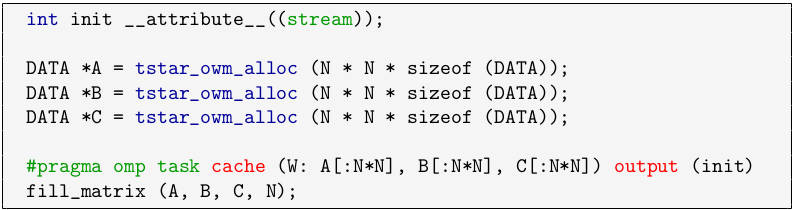
\includegraphics[width=5.122in,height=1.361in]{img44.png}
\par}

{\centering\selectlanguage{english}\sffamily\bfseries
\label{bkm:Ref388170820}Fig.
\stepcounter{Figure}{\theFigure} -- Matrix product -- input.
\par}

{\centering 
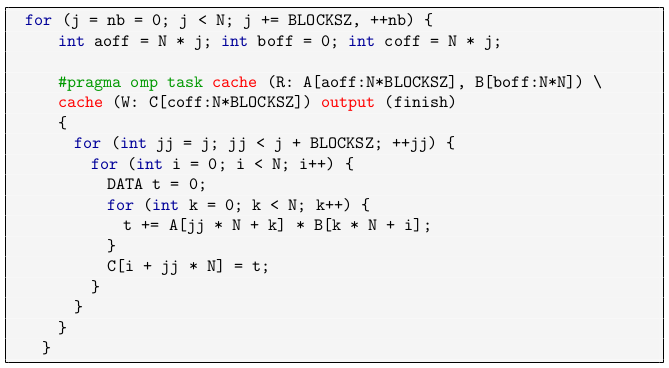
\includegraphics[width=4.2362in,height=2.3354in]{img45.png}
\par}

{\centering\selectlanguage{english}\sffamily\bfseries
\label{bkm:Ref388170843}Fig.
\stepcounter{Figure}{\theFigure} -- Matrix product -- input.
\par}

{\selectlanguage{english}
The main computations are done in the following phase. Fig. 29 shows the
code for matrix multiplication. The matrix is divided into blocks, each
thread caches BLOCKSZ rows of matrix A, and the entire matrix B in read
mode, and BLOCKSZ rows of matrix C in write mode. Once the thread is
executed, it computes
ABLOCKSZ{\textbullet}N{\textbullet}BN{\textbullet}N =
CBLOCKSZ{\textbullet}N. At the end of each thread, the modification to
matrix C is published and thus available for reading by other threads.
Each task created in this phase writes a single value to stream
\textit{finish}. Stream finish acts as a waiting barrier in the last
task, which will wait for the termination of all threads created in
this phase.}

{\centering 
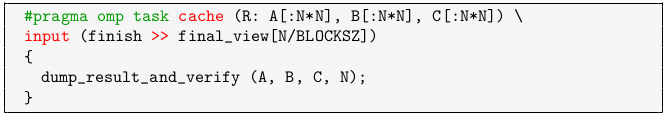
\includegraphics[width=5.361in,height=0.9071in]{img46.png}
\par}

{\centering\selectlanguage{english}\sffamily\bfseries
\label{bkm:Ref388170857}Fig.
\stepcounter{Figure}{\theFigure} -- Matrix product -- input.
\par}

{\selectlanguage{english}
Fig. 30 shows the final thread, which waits for the termination of all
the threads created in phase two. Once all the computations are done,
it will output the results and do the verification if necessary. Stream
finish acts as a barrier, waits for N/BLOCKSZ inputs from stream
finish. Each thread created in phase two writes to stream finish once
finished.}

\subsection[Further references to more in{}-depths]{Further references
to more in-depths}
{\selectlanguage{english}
The semantics, dedicated memory model and coherence protocol for OWM
will be the subject of a joint publication of the project partners. The
Master thesis of Fran\c{c}ois Gindraud is currently the most accurate
information and is available on request. We have studied four
benchmarks with OWM support: matrix multiplication, sparse LU, Gauss
Seidel and Viola \& Jones (pedestrian detection); those benchmarks are
validated with COTSon{\textquotesingle}s TSUF branch.}

\section[Research Use Case from MSFT]{Research Use Case from MSFT}
{\selectlanguage{english}
This section demonstrates how to run the TERAFLUX operating system
prototype that was developed to support research and experimentation
with the various parallel, distributed and reliable execution
algorithms that are suggested in TERAFLUX. Specifically, the operating
system supports execution of a distributed application over the
many-core device using dataflow threads, it was designed to handle core
soft errors with Double Execution mechanism and can handle node
hard-failures such that the application can transparently continue
execution as the work that was pending on the failed node is recovered
and executed by the remaining nodes.}

{\selectlanguage{english}
The system is simulated over COTSon (running a SimNow instance for each
of the nodes) with a slightly modified version of TSUF, which
implements a shared memory mechanism with a weak consistency model
similar to acquire/release. This shared memory is the only mechanism
utilized by the operating system for inter-node communications and
shared data.}

\subsection[Goal of the experiment or example]{Goal of the experiment or
example}
{\selectlanguage{english}
This experiment launches a distributed Fibonacci sequence computation
over the TERAFLUX operating system. Its goal is to demonstrate how the
operating system executes a massively parallel application made of
dataflow threads over all of the cores in the system.}

{\selectlanguage{english}
During execution, the simulation displays the operations performed by
the run-time and the user code in the virtual monitor of each SimNow
instance, additionally, the output is logged and can be examined after
execution. Soft-errors can be injected randomly to the results to
demonstrate the Double Execution in action, and complete node failure
can be triggered by the user to watch the recovery mechanism.}

{\selectlanguage{english}
Various compile flags control some of the run-time mechanisms (e.g.,
scheduling algorithm, Double Execution, etc.), and what type of log
messages are seen.}

\subsection[Location of the involved files]{Location of the involved
files}
{\selectlanguage{english}
The runtime files and sample application are contained in the following
folder:}

\begin{flushleft}
\tablehead{}
\begin{supertabular}{|m{6.29346in}|}
\hline
\selectlanguage{english}
\texttt{\$COTSONHOME/branches/tflux-test/tfos/}\\\hline
\end{supertabular}
\end{flushleft}
{\selectlanguage{english}
Where \textbf{COTSONHOME }is an environmental variable identifying the
path where the COTSon simulator was checked out with: }

\begin{flushleft}
\tablehead{}
\begin{supertabular}{|m{6.29346in}|}
\hline
\selectlanguage{english}\ttfamily \$ svn co
https://svn.code.sf.net/p/cotson/code/ \$COTSONHOME\\\hline
\end{supertabular}
\end{flushleft}
\subsection[Detailed instructions to start]{Detailed instructions to
start}
{\selectlanguage{english}
To run this example first checkout and build COTSon, then go to the
\textit{tfos-tsuf} folder mentioned above:}

\begin{flushleft}
\tablehead{}
\begin{supertabular}{|m{6.29346in}|}
\hline
\selectlanguage{english} \texttt{\$ cd
\$COTSONHOME/branches/tflux-test/tfos/}\\\hline
\end{supertabular}
\end{flushleft}
{\selectlanguage{english}
Now start the simulation by executing:}

\begin{flushleft}
\tablehead{}
\begin{supertabular}{|m{6.29346in}|}
\hline
\selectlanguage{english} \texttt{\$ make run\_multi}\\\hline
\end{supertabular}
\end{flushleft}
{\selectlanguage{english}
After startup, the default simulation view will display general
information about the node and list several commands (e.g., show logs,
test node failure, etc.) that can be interactively triggered by the
user with keyboard command on the SimNow window.}

{\selectlanguage{english}
Some parameters can be configured similarly to those in TSUF, for
example the number of nodes in the system is specified in
\textit{os-tests/tsu\_multi.lua}:}

\begin{flushleft}
\tablehead{}
\begin{supertabular}{|m{6.29346in}|}
\hline
\selectlanguage{english}\ttfamily cluster\_nodes=4\\\hline
\end{supertabular}
\end{flushleft}
{\selectlanguage{english}
The number of cores in each node is specified by the bsd file used:}

\begin{flushleft}
\tablehead{}
\begin{supertabular}{|m{6.29346in}|}
\hline
{\selectlanguage{english}
\texttt{{}-{}-use\_bsd({\textquotesingle}4p.bsd{\textquotesingle})}}

{\selectlanguage{english}\ttfamily
use\_bsd({\textquotesingle}16p.bsd{\textquotesingle})}

\selectlanguage{english}\ttfamily
{}-{}-use\_bsd({\textquotesingle}32p.bsd{\textquotesingle})\\\hline
\end{supertabular}
\end{flushleft}
{\selectlanguage{english}
To test node crashes it is recommended to have more than 4 cores in each
node. Notice that the bsd{\textquoteright}s with large number of cores
are not created using the default build configuration, they can be
downloaded from:}

\begin{flushleft}
\tablehead{}
\begin{supertabular}{|m{6.3031597in}|}
\hline
\selectlanguage{english}\ttfamily
https://upload.teraflux.eu/uploads/BSDS/bsds\_images\_initialized\_for\_karmc64\_1Ghz.tar.gz\\\hline
\end{supertabular}
\end{flushleft}
{\selectlanguage{english}
Some other parameters are specified in \textit{os-tests/Makefile}:}

\begin{flushleft}
\tablehead{}
\begin{supertabular}{|m{6.29346in}|}
\hline
{\selectlanguage{english}\ttfamily OWMSZ=67108864 \# Size of the shared
region.}

{\selectlanguage{english}\ttfamily SZ=44 \# Parameter for the
application (e.g. Fibonacci number).}

\selectlanguage{english}\ttfamily \#NT=32 \# Number of TSUF workers.
Leave undefined to use the number of cores.\\\hline
\end{supertabular}
\end{flushleft}
{\selectlanguage{english}
Several parameters are specified as compile time flags. Some flags
control the nature of the dataflow jobs. For example:}

\begin{flushleft}
\tablehead{}
\begin{supertabular}{|m{6.29346in}|}
\hline
{\selectlanguage{english}\ttfamily \#define DOUBLE\_EXECUTION}

\selectlanguage{english}\ttfamily //\#define INJECT\_CORRUPTIONS\\\hline
\end{supertabular}
\end{flushleft}
{\selectlanguage{english}
The above macro is used to determine whether to globally enable Double
Execution, and whether to randomly corrupt some of the threads results
to see the mechanism in action.}

{\selectlanguage{english}
The following macro defines whether to include the actual job binary in
the control message or only its name: }

\begin{flushleft}
\tablehead{}
\begin{supertabular}{|m{6.29346in}|}
\hline
\selectlanguage{english}\ttfamily \#define SEND\_JOB\_NAMES\\\hline
\end{supertabular}
\end{flushleft}
{\selectlanguage{english}
When it{\textquoteright}s disabled, each job message is self-contained
and allows immediate execution on any node without access to shared
storage (of the precompiled jobs), at the cost of possibly sending the
same binary code many times. Although jobs are usually small (100-200
bytes for Fibonacci) this can be avoided by sending a small job
identifier instead of the binary code, later used to load the job from
the common file system (subsequent requests are loaded from cache).}

{\selectlanguage{english}
Simple scheduling algorithms can be chosen with the macros:}

\begin{flushleft}
\tablehead{}
\begin{supertabular}{|m{6.29346in}|}
\hline
{\selectlanguage{english}\ttfamily // Prefer to schedule on the local
node until memory usage is high, then}

{\selectlanguage{english}\ttfamily // a secondary method is used. If
this is not defined, the method chosen below is // immediately used.}

{\selectlanguage{english}\ttfamily \#define PREFER\_LOCAL}

{\selectlanguage{english}\ttfamily // Define only one of the following:}

{\selectlanguage{english}\ttfamily //\#define RANDOM\_SCHED\_POLICY}

\selectlanguage{english}\ttfamily \#define
UNIFORM\_DISTRIBUTION\_POLICY\\\hline
\end{supertabular}
\end{flushleft}
{\selectlanguage{english}
Those are very simple but demonstrate how the information gathered from
heartbeats can be used to help load balancing among nodes.}

\subsection[Expected output]{Expected output}
{\selectlanguage{english}
When launched, node instances will open in SimNow windows and display
the simulation progress:}


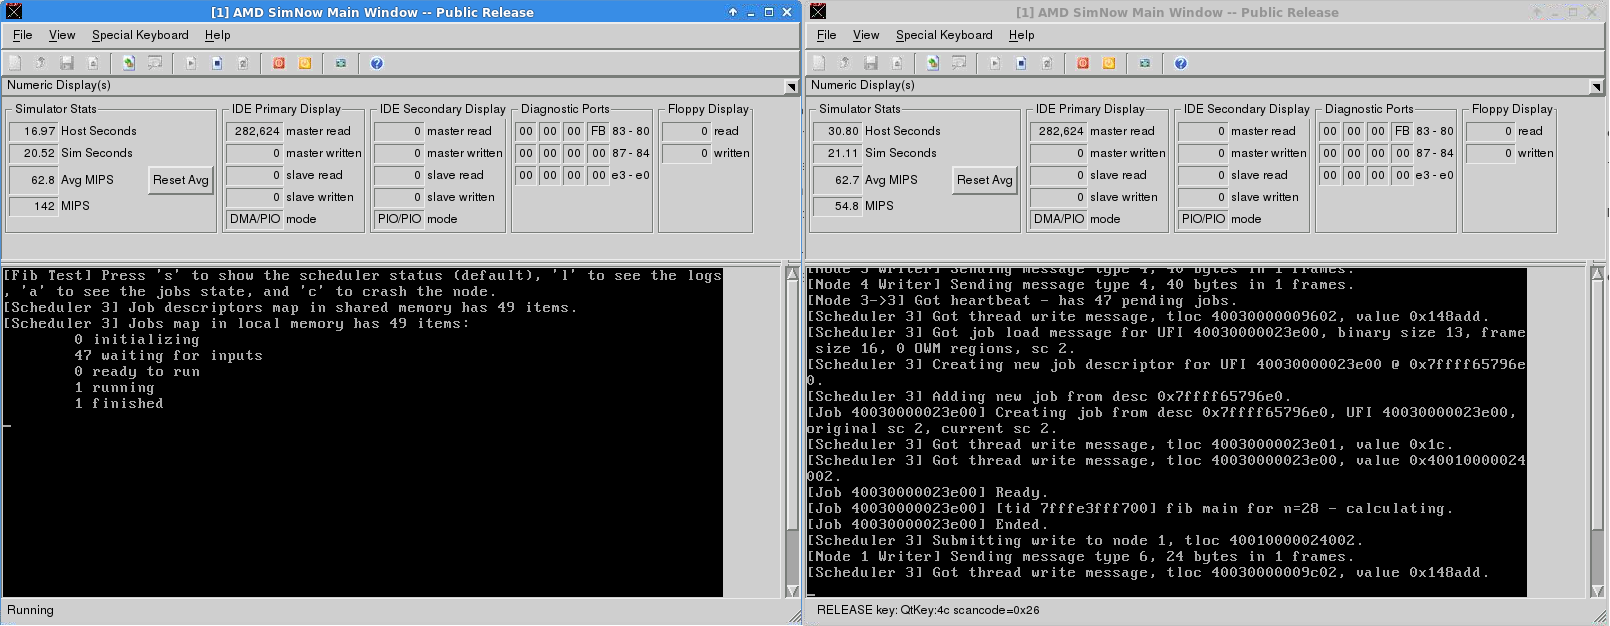
\includegraphics[width=6.2547in,height=2.4319in]{img47.png}


{\centering\selectlanguage{english}\sffamily\bfseries
Fig.
\stepcounter{Figure}{\theFigure} -- Two nodes (two SimNow instances)
running on the COTSon simulator.
\par}

{\selectlanguage{english}
When the simulation completes, the output of each node can be examined
in the \textit{stdout} log files, the output of node 1 could be for
example:}

\begin{flushleft}
\tablehead{}
\begin{supertabular}{|m{6.4018598in}|}
\hline
{\selectlanguage{english} \texttt{[[Manager 1] Simulation parameters:}}

{\selectlanguage{english}\ttfamily [Manager 1] \ \ 16 cores in 4 nodes
with 4 cores each.}

{\selectlanguage{english}\ttfamily [Manager 1] \ \ 64MB public shared
memory, 16MB per node.}

{\selectlanguage{english}\ttfamily [Manager 1] \ \ 4*1MB message queues,
leaves 12MB for dynamic allocation.}

{\selectlanguage{english}\ttfamily [Manager 1] Starting service thread,
ip 0x4202e0.}

{\selectlanguage{english}\ttfamily [Scheduler 1] Dynamic allocation area
rounded from 0x7ffff46f4140 to 0x7ffff46f5000, size 12MB.}

{\selectlanguage{english}\ttfamily [Manager 1] Starting service thread,
ip 0x40c360.}

{\selectlanguage{english}\ttfamily [Test] Computing fibonacci(41).}

{\selectlanguage{english}\ttfamily [Scheduler 1] Starting message pump.}

{\selectlanguage{english}\ttfamily [Scheduler 1] Submitting job
fib\_reporter\_job with UFI 10010000000200.}

{\selectlanguage{english}\ttfamily [Node 1 Writer] Sending message type
1, 73 bytes in 2 frames.}

{\selectlanguage{english}\ttfamily [Scheduler 1] Submitting job
fib\_main\_job with UFI 10010000000400.}

{\selectlanguage{english}\ttfamily [Node 1 Writer] Sending message type
1, 77 bytes in 2 frames.}

{\selectlanguage{english}\ttfamily [Scheduler 1] Finalizing 0: Write
destination updated from VFP 200 to UFI 10010000000400.}

{\selectlanguage{english}\ttfamily [Scheduler 1] Submitting write to
node 1, tloc 10010000000400.}

{\selectlanguage{english}\ttfamily [Node 1 Writer] Sending message type
6, 24 bytes in 1 frames.}

{\selectlanguage{english}\ttfamily [Scheduler 1] Finalizing 0: Write
destination updated from VFP 200 to UFI 10010000000400.}

{\selectlanguage{english}\ttfamily [Scheduler 1] Submitting write to
node 1, tloc 10010000000401.}

{\selectlanguage{english}\ttfamily [Node 1 Writer] Sending message type
6, 24 bytes in 1 frames.}

{\selectlanguage{english}\ttfamily [Scheduler 1] Got job load message
for UFI 10010000000200, binary size 17, frame size 8, sc 1.}

{\selectlanguage{english}\ttfamily [Scheduler 1] Creating new job
descriptor for UFI 10010000000200 @ 0x7ffff46f5140.}

{\selectlanguage{english}\ttfamily [Job 10010000000200] Creating job
from desc 0x7ffff46f5140, UFI 10010000000200, original sc 1, current sc
1.}

{\selectlanguage{english}\ttfamily [BinariesStore] Adding job binary:
fib\_reporter\_job, 142 bytes.}

{\selectlanguage{english}\ttfamily [Scheduler 1] Got job load message
for UFI 10010000000400, binary size 13, frame size 16 , sc 2.}

{\selectlanguage{english}\ttfamily [Scheduler 1] Creating new job
descriptor for UFI 10010000000400 @ 0x7ffff46f51e0.}

{\selectlanguage{english}\ttfamily [Job 10010000000400] Creating job
from desc 0x7ffff46f51e0, UFI 10010000000400, original sc 2, current sc
2.}

{\selectlanguage{english}\ttfamily [BinariesStore] Adding job binary:
fib\_main\_job, 618 bytes.}

{\selectlanguage{english}\ttfamily [Scheduler 1] Got thread write
message, tloc 10010000000400, value 0x10010000000200.}

{\selectlanguage{english}\ttfamily [Scheduler 1] Got thread write
message, tloc 10010000000401, value 0x29.}

{\selectlanguage{english}\ttfamily [Job 10010000000400] Ready.}

{\selectlanguage{english}\ttfamily [Job 10010000000400] [tid
7fffe3fff700] fib main for n=41 - spawning.}

{\selectlanguage{english}\ttfamily [Job 10010000000400] Ended.}

{\selectlanguage{english}\ttfamily ...}

{\selectlanguage{english}\ttfamily [Scheduler 1] Got thread write
message, tloc 10010000000200, value 0x9de8d6d.}

{\selectlanguage{english}\ttfamily [Job 10010000000200] Ready.}

{\selectlanguage{english}\ttfamily [Job 10010000000200] [tid
7fffe3fff700] report: fib result = 165580141}

{\selectlanguage{english}\ttfamily [Job 10010000000200] [tid
7fffe3fff700] Exit requested.}

{\selectlanguage{english}\ttfamily [Job 10010000000200] Ended.}

{\selectlanguage{english}\ttfamily [Scheduler 1] Sending termination
requests...}

{\selectlanguage{english}\ttfamily [Node 1 Writer] Sending message type
7, 8 bytes in 1 frames.}

{\selectlanguage{english}\ttfamily [Node 2 Writer] Sending message type
7, 8 bytes in 1 frames.}

{\selectlanguage{english}\ttfamily [Node 3 Writer] Sending message type
7, 8 bytes in 1 frames.}

{\selectlanguage{english}\ttfamily [Node 4 Writer] Sending message type
7, 8 bytes in 1 frames.}

{\selectlanguage{english}\ttfamily [Node 1-{\textgreater}1] Got
terminate message.}

\selectlanguage{english}\ttfamily [Scheduler 1] Exiting.\\\hline
\end{supertabular}
\end{flushleft}
{\selectlanguage{english}
If a node (node 3 in the example) was killed by user input, the recovery
node (node 1 was chosen in the example) will begin to take over and
process the work of the failed node and display:}

{\centering 
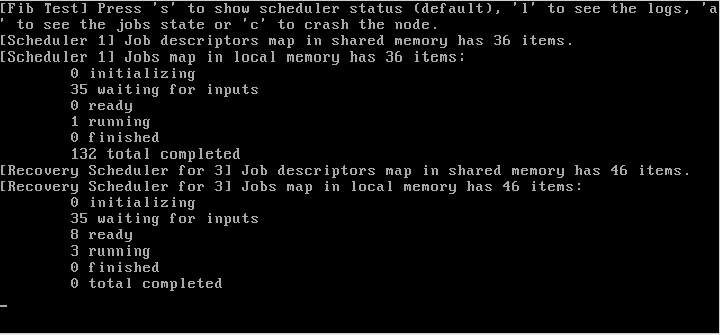
\includegraphics[width=4.1555in,height=1.7453in]{img48.png}
\par}

{\centering\selectlanguage{english}\sffamily\bfseries
Fig.
\stepcounter{Figure}{\theFigure} -- Output of the simulation when a
node in the system fails.
\par}

{\selectlanguage{english}
The log should show:}

\begin{flushleft}
\tablehead{}
\begin{supertabular}{|m{6.4018598in}|}
\hline
{\selectlanguage{english}\ttfamily ...}

{\selectlanguage{english}\ttfamily [Watchdog] Node 3 probably died, no
heart beat received in the last 189 milliseconds.}

{\selectlanguage{english}\ttfamily [Manager 1] Starting recovery
procedure for node 3.}

{\selectlanguage{english}\ttfamily [Manager 1] Starting service thread,
ip 0x406d60.}

{\selectlanguage{english}\ttfamily [Recovery Scheduler for 3] Checking
shared segment sanity...}

{\selectlanguage{english}\ttfamily [Recovery Scheduler for 3] Job
descriptors map in shared memory has 37 items.}

{\selectlanguage{english}\ttfamily [Recovery Scheduler for 3] Adding new
job from desc 0x7ffff65793c0.}

{\selectlanguage{english}\ttfamily [Job 1003000000bc00] Creating job
from desc 0x7ffff65793c0, UFI 1003000000bc00, original sc 2, current sc
0.}

{\selectlanguage{english}\ttfamily [Job 1003000000bc00] Ready.}

{\selectlanguage{english}\ttfamily [Job 1003000000bc00] [tid
7fffe3fff700] fib main for n=29 - calculating.}

{\selectlanguage{english}\ttfamily [Recovery Scheduler for 3] Adding new
job from desc 0x7ffff65791e0.}

{\selectlanguage{english}\ttfamily [Job 2003000000e600] Creating job
from desc 0x7ffff65791e0, UFI 2003000000e600, original sc 2, current sc
2.}

{\selectlanguage{english}\ttfamily [Recovery Scheduler for 3] Adding new
job from desc 0x7ffff6579140.}

{\selectlanguage{english}\ttfamily [Job 30030000000c00] Creating job
from desc 0x7ffff6579140, UFI 30030000000c00, original sc 3, current sc
2.}

{\selectlanguage{english}\ttfamily ... {\textless}More recovered jobs
information{\textgreater} ...}

{\selectlanguage{english}\ttfamily [Recovery Scheduler for 3] Has 46
jobs in local memory:}

{\selectlanguage{english}\ttfamily \ \ 0 initializing}

{\selectlanguage{english}\ttfamily \ \ 35 waiting for inputs}

{\selectlanguage{english}\ttfamily \ \ 8 ready}

{\selectlanguage{english}\ttfamily \ \ 3 running}

{\selectlanguage{english}\ttfamily \ \ 0 finished}

{\selectlanguage{english}\ttfamily \ \ 0 total completed}

{\selectlanguage{english}\ttfamily [Recovery Scheduler for 3] Starting
message pump.}

{\selectlanguage{english}\ttfamily [Recovery Scheduler for 3] Got job
load message for UFI 1003000000c200, binary size 13, frame size 16, sc
2.}

{\selectlanguage{english}\ttfamily [Recovery Scheduler for 3] Creating
new job descriptor for UFI 1003000000c200 @ 0x7ffff657a860.}

{\selectlanguage{english}\ttfamily [Job 1003000000c200] Creating job
from desc 0x7ffff657a860, UFI 1003000000c200, original sc 2, current sc
2.}

{\selectlanguage{english}\ttfamily [Recovery Scheduler for 3] Got thread
write message, tloc 2003000000e601, value 0x1e.}

\selectlanguage{english}\ttfamily ... {\textless}More recovered messages
processing{\textgreater} ...\\\hline
\end{supertabular}
\end{flushleft}
{\selectlanguage{english}
If Double Execution and random error injections are enabled, an injected
soft-error will produce output similar to the following:}

{\centering 
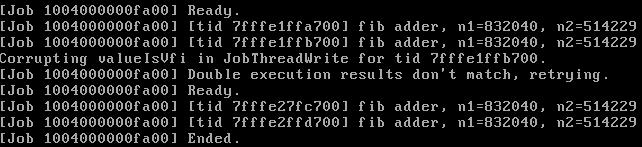
\includegraphics[width=4.1055in,height=0.9429in]{img49.png}
\par}

{\centering\selectlanguage{english}\sffamily\bfseries
Fig.
\stepcounter{Figure}{\theFigure} -- Double Execution of dataflow
threads, and the corresponding verification output.
\par}

{\selectlanguage{english}
This is a simple implementation of Double Execution; each job is
executed twice (notice the different \textit{tid} on each execution),
and the results are not committed to the shared memory until the
results of both threads are ready and compared equal. When an error is
injected, the mechanism detects it and launches the job again on two
threads.}

\subsection[Further references to more in{}-depths]{Further references
to more in-depths}
{\selectlanguage{english}
For more details on the operating system structure and its mechanisms
that support the reliable execution of Data-Flow threads while assuming
incoherent shared memory and possibility of node hard-failures. This
information is also contained in the \textit{TFOS.pdf} document in the
source folder.}

\section[Research Use Case from THALES]{Research Use Case from THALES}
{\selectlanguage{english}
This section shows a subset of the experiments performed on the
applications provided by Thales, to evaluate the TERAFLUX architecture
and associated tools in an industrial context. }

{\selectlanguage{english}
THALES provided the following two use-cases: the Radar application and
the Pedestrian Detection application. This document focuses on the
later one, the Radar application, providing some easy instructions for
its installation and test. }

{\selectlanguage{english}
The Radar application is an airborne radar application embedded in
planes to detect the position and radial speed of another flying target
despite the presence of jamming devices. It is based on the Space-Time
Adaptive Processing (STAP) algorithm. This application is characterized
by:}

\begin{itemize}
\item {\selectlanguage{english}
Real-time constraints expressed in the form of throughput requirements;}
\item {\selectlanguage{english}
The pure dataflow behavior of a signal processing application;}
\item {\selectlanguage{english}
But very large data (5\textsuperscript{th} dimensional data) being
transferred between each task/filter;}
\item {\selectlanguage{english}
T necessity to manipulate this data (e.g., rotate, transpose, etc.) for
each filter to benefits from cache locality;}
\end{itemize}
\subsection[Goal of the experiment or example]{Goal of the experiment or
example}
{\selectlanguage{english}
The goals of the experiments are: first, to evaluate the scalability of
the proposed architecture and associated dataflow execution models in
the context of real-time applications, selecting one application that
is very dataflow friendly (radar).}

{\selectlanguage{english}
Second, to evaluate the ergonomics of the tools and associated dataflow
languages, and to evaluate the cost of porting legacy single-core
applications to the TERAFLUX platform, including the parallelization
costs versus the obtained speedups, using the available execution
models.}

{\selectlanguage{english}
Third, to estimate what are the best parallelization options for porting
classification algorithms and signal-processing algorithms to
teradevices. In the case of the Radar application its parallelization
is quite straightforward alongside the dataflow pipeline.}

\subsection[Location of the involved files]{Location of the involved
files}
{\selectlanguage{english}
\ To start, the \textit{tsuf} version of TSU must be checked out with:}

\begin{flushleft}
\tablehead{}
\begin{supertabular}{|m{6.29346in}|}
\hline
\selectlanguage{english} \texttt{\$ svn co
}\url{https://svn.code.sf.net/p/cotson/code/branches/tflux-test/tsuf/}\texttt{
\$TSUF\_HOME}\\\hline
\end{supertabular}
\end{flushleft}
{\selectlanguage{english}
The Radar benchmark (STAP) can be checked out with:}

\begin{flushleft}
\tablehead{}
\begin{supertabular}{|m{6.29346in}|}
\hline
\selectlanguage{english} \texttt{\$ svn co
https://svn.code.sf.net/p/teraflux-stap/code \$STAP\_HOME}\\\hline
\end{supertabular}
\end{flushleft}
\subsection[Detailed instructions to start]{Detailed instructions to
start}
{\selectlanguage{english}
\ Before using the Radar application the following steps must be
followed:}

\begin{enumerate}
\item {\selectlanguage{english}
Checkout, build and install COTSON;}
\item {\selectlanguage{english}
Checkout, build and install the TSUF version of the distributed Thread
Scheduling Unit (TSU);}
\item {\selectlanguage{english}
Checkout, build and install the SimNow simulator;}
\item {\selectlanguage{english}
Checkout, build and install the TERAFLUX-version of the OpenStream
compiler;}
\item {\selectlanguage{english}
(Optional) Checkout, build and install the OmpSs compiler (not
compatible with the Thread Scheduling Unit models);}
\end{enumerate}
{\selectlanguage{english}
A \texttt{Makefile} is included with the application. Simply type
\texttt{make} to see all the available options. The \texttt{makefile}
should be updated with the paths of the previously installed software
(i.e., COTSon, SimNow, OpenStream and optionally OmpSs). Below the
options that concern the OpenStream with TSU support version of the
Radar application:}

\begin{flushleft}
\tablehead{}
\begin{supertabular}{|m{6.29346in}|}
\hline
{\selectlanguage{english} \texttt{\$ make
{\textless}stap-os-cotson{\textbar}run-os-cotson-small{\textbar}run-os-cotson-large{\textbar}run-os-cotson-huge{\textbar}}\texttt{run-os-cotson-multi-small{\textbar}run-os-cotson-multi-large{\textbar}run-os-cotson-multi-huge{\textbar}clean-os-cotson{\textgreater}}}

{\selectlanguage{english} \texttt{\$ \ \ Build OpenStream version of the
application.}}

{\selectlanguage{english} \texttt{\$ \ \ Run COTSON OpenStream version
on small input.}}

{\selectlanguage{english} \texttt{\$ \ \ Run COTSON OpenStream version
on large input.}}

{\selectlanguage{english} \texttt{\$ \ \ Run COTSON OpenStream version
on huge input.}}

{\selectlanguage{english} \texttt{\$ \ \ Run multi COTSON OpenStream
version on small input.}}

{\selectlanguage{english} \texttt{\$ \ \ Run multi COTSON OpenStream
version on large input.}}

{\selectlanguage{english} \texttt{\$ \ \ Run multi COTSON OpenStream
version on huge input.}}

\selectlanguage{english} \texttt{\$ \ \ Clean files created by the
OpenStream application.}\\\hline
\end{supertabular}
\end{flushleft}
{\selectlanguage{english}
To launch a single node TSU execution with the small dataset just launch
\textit{make run-os-cotson-small}. The \textit{{}-cotson-multi-}
variations will execute a multiple node TSU simulation. Three different
input sets are provided for evaluation.}

{\selectlanguage{english}
The sources provide a \textit{\$STAP\_HOME/resources} folder with the
TSU configuration files, the default use machine configurations
provided by COTSon, modify them to use larger/smaller configurations.}

\subsection[\ Expected output]{\foreignlanguage{english}{\ }Expected
output}
{\selectlanguage{english}
The Radar application doesn{\textquoteright}t provide any visual output.
It takes a radar signal and detects moving objects. When running the
TERAFLUX version of the application with the \texttt{make
run-os-cotson-{\textless}small{\textbar}large{\textbar}huge{\textgreater}}
command it generates as output the detected objects in a text file with
the name of the selected input set:
\texttt{{\textless}small{\textbar}large{\textbar}huge{\textgreater}.txt}.
The \texttt{Makefile} command
\texttt{run-os-cotson-{\textless}small{\textbar}large{\textbar}huge{\textgreater}}
places the output file in
\texttt{run/{\textless}os-cotson{\textgreater}}. The user can check
that the result is correct by comparing this output against the output
of the sequential single core x86 version that can be run with the
\texttt{make
run-seq-{\textless}small{\textbar}large{\textbar}huge{\textgreater}}
command that generates its output file in \texttt{run/seq }folder.}

{\selectlanguage{english}
Some speedup results for the Radar application observed with different
configurations (4 cores per node) of the TERAFLUX machine compared to
the sequential version are reported in table 2.}

{\centering\selectlanguage{english}\sffamily\bfseries
Table
\stepcounter{Table}{\theTable} -- Radar application speedup against
sequential execution
\par}

\begin{center}
\tablehead{}
\begin{supertabular}{|m{0.47885987in}|m{0.6434598in}|m{1.1025599in}|m{0.9129598in}|}
\hline
\multicolumn{4}{|m{3.37406in}|}{\centering
\selectlanguage{english}\bfseries Dataset}\\\hline
\selectlanguage{english}\bfseries Cores &
\centering \selectlanguage{english}\bfseries Small &
\centering \selectlanguage{english}\bfseries Large &
\centering\arraybslash \selectlanguage{english}\bfseries Huge\\\hline
\centering \selectlanguage{english} 4 &
\centering \selectlanguage{english} 3.48 &
\centering \selectlanguage{english} 3.48 &
\centering\arraybslash \selectlanguage{english} 3.48\\\hline
\centering \selectlanguage{english} 8 &
\centering \selectlanguage{english} 6.22 &
\centering \selectlanguage{english} 6.24 &
\centering\arraybslash \selectlanguage{english} 6.26\\\hline
\centering \selectlanguage{english} 16 &
\centering \selectlanguage{english} 10.28 &
\centering \selectlanguage{english} 10.41 &
\centering\arraybslash \selectlanguage{english} 10.44\\\hline
\centering \selectlanguage{english} 32 &
\centering \selectlanguage{english} 14.33 &
\centering \selectlanguage{english} 14.59 &
\centering\arraybslash \selectlanguage{english} 14.63\\\hline
\centering \selectlanguage{english} 64 &
\centering \selectlanguage{english} 16.96 &
\centering \selectlanguage{english} 18.08 &
\centering\arraybslash \selectlanguage{english} 17.92\\\hline
\end{supertabular}
\end{center}
\subsection[\ Further references to more
in{}-depths]{\foreignlanguage{english}{\ }Further references to more
in-depths}
{\selectlanguage{english}
none.}

\section[Research Use Case from UAU]{Research Use Case from UAU}
{\selectlanguage{english}
This section shows a simplified experiment to investigate the
performance overhead induced by the fault detection mechanisms
developed in TERAFLUX. }

\subsection[Goal of the experiment ]{Goal of the experiment }
{\selectlanguage{english}
The goal of this experiment is to show the performance overhead of
pessimistic and optimistic Double Execution of \textit{Fibonacci(31)}
for one TERAFLUX node with 4 cores. Location of the involved files }

{\selectlanguage{english}
To start, the fault-tolerant version of the Thread Scheduling Unit (TSU)
must be checked out with:}

\begin{flushleft}
\tablehead{}
\begin{supertabular}{|m{6.29346in}|}
\hline
\selectlanguage{english}\ttfamily \$ svn co
https://svn.code.sf.net/p/cotson/code/branches/tflux-test/ft-tsu/
\$FT\_TSU\_HOME\\\hline
\end{supertabular}
\end{flushleft}
{\selectlanguage{english}
The fault-tolerant version of the TSU (\textit{tflux\_tsu.cpp}), the
used cpu timer (\textit{timer\_uau.cpp}), and the COTSon configuration
skeleton (\textit{tsu\_bench.lua}) used for the experiment can all be
found in \textit{\$FT\_TSU\_HOME.}}

{\selectlanguage{english}
The benchmarks are stored in:}

\begin{flushleft}
\tablehead{}
\begin{supertabular}{|m{6.29346in}|}
\hline
\selectlanguage{english}\ttfamily \$ FT\_TSU\_HOME/examples\\\hline
\end{supertabular}
\end{flushleft}
\subsection[Detailed instructions to start ]{Detailed instructions to
start }
{\selectlanguage{english}
Before the experiment can be started, the required dependencies must be
installed by:}

\begin{flushleft}
\tablehead{}
\begin{supertabular}{|m{6.29346in}|}
\hline
\selectlanguage{english} \texttt{\$ FT\_TSU\_HOME/configure
--{}-simnow\_dir /path/to/simnow}\\\hline
\end{supertabular}
\end{flushleft}
{\selectlanguage{english}
The \textit{configure} script will perform the following tasks:}

\begin{enumerate}
\item {\selectlanguage{english}
Checkout and build the COTSon simulator;}
\item {\selectlanguage{english}
Build and link all required files in \textit{\$FT\_TSU\_HOME};}
\end{enumerate}
{\selectlanguage{english}
Afterwards the experiment can be started with:}

\begin{flushleft}
\tablehead{}
\begin{supertabular}{|m{6.29346in}|}
\hline
\selectlanguage{english} \texttt{\$ FT\_TSU\_HOME/run\_example
--{}-res\_folder /path/to/results\_folder}\\\hline
\end{supertabular}
\end{flushleft}
{\selectlanguage{english}
Where the \textit{res\_folder} option describes the folder where the
results of the experiments will be stored.}

\subsection[Expected output]{Expected output}
{\selectlanguage{english}
After the experiment has finished the execution, the raw output files of
the simulator runs can be found in the \textit{res\_folder}.}

{\selectlanguage{english}
Finally, the simulator outputs can be aggregated by a script, which
creates an \textit{example\_results.csv }file in the\textit{
res\_folder}:}

\begin{flushleft}
\tablehead{}
\begin{supertabular}{|m{6.29346in}|}
\hline
\selectlanguage{english} \texttt{\$
FT\_TSU\_HOME/build\_example\_table.sh --{}-res\_folder
/path/to/results\_folder}\\\hline
\end{supertabular}
\end{flushleft}
{\selectlanguage{english}
The following tables show the results extracted from the
\textit{example\_results.csv} for regular dataflow execution (Table 3),
pessimistic Double Execution (Table 4), and optimistic Double Execution
(Table 5). For a better classification of the example execution, we
also present the results for TERAFLUX nodes with 1, 2, 8, 16, and 32
cores. The results extracted from the \textit{example\_results.csv} are
highlighted in yellow. Based on the execution times, the run-time
overhead for pessimistic and optimistic Double Execution (compared to
the baseline regular execution) can be additionally calculated. Since
the objective is to depict the overhead solely induced by Double
Execution, the overhead has been normalized to the regular execution
time using half of the cores.}

{\centering\selectlanguage{english}\sffamily\bfseries
Table
\stepcounter{Table}{\theTable} -- Node Utilization and Execution Time
of the Baseline Dataflow Execution
\par}

\begin{center}
\tablehead{}
\begin{supertabular}{|m{1.0268599in}|m{1.2504599in}|m{1.2455599in}|}
\hline
\selectlanguage{english}\bfseries Cores &
\centering \selectlanguage{english}\bfseries Node Utilization [\%] &
\centering\arraybslash \selectlanguage{english}\bfseries Execution Time
[ns]\\\hline
\selectlanguage{english}\bfseries 1 &
\centering \selectlanguage{english}\bfseries 99.9 &
\centering\arraybslash \selectlanguage{english}\bfseries
34,762,104\\\hline
\selectlanguage{english}\bfseries 2 &
\centering \selectlanguage{english}\bfseries 99.9 &
\centering\arraybslash \selectlanguage{english}\bfseries
17,769,355\\\hline
\selectlanguage{english}\bfseries 4 &
\centering \selectlanguage{english}\bfseries 99.7 &
\centering\arraybslash \selectlanguage{english}\bfseries
9,209,017\\\hline
\selectlanguage{english}\bfseries 8 &
\centering \selectlanguage{english}\bfseries 98.4 &
\centering\arraybslash \selectlanguage{english}\bfseries
4,864,722\\\hline
\selectlanguage{english}\bfseries 16 &
\centering \selectlanguage{english}\bfseries 96.7 &
\centering\arraybslash \selectlanguage{english}\bfseries
2,550,796\\\hline
\end{supertabular}
\end{center}

\bigskip

{\centering\selectlanguage{english}\sffamily\bfseries
Table
\stepcounter{Table}{\theTable} -- Node Utilization and Execution Time
of Pessimistic Double Execution
\par}

\begin{center}
\tablehead{}
\begin{supertabular}{|m{1.0268599in}|m{1.2504599in}|m{1.2386599in}|m{1.2455599in}|}
\hline
\selectlanguage{english}\bfseries Cores &
\centering \selectlanguage{english}\bfseries Node Utilization[\%] &
\centering \selectlanguage{english}\bfseries Execution Time[ns] &
\centering\arraybslash \selectlanguage{english}\bfseries Runtime
Overhead [\%]\\\hline
\selectlanguage{english}\bfseries 2 &
\centering \selectlanguage{english}\bfseries 99.2 &
\centering \selectlanguage{english}\bfseries 35,751,164 &
\centering\arraybslash \selectlanguage{english}\bfseries 2.8\\\hline
\selectlanguage{english}\bfseries 4 &
\centering \selectlanguage{english}\bfseries 99.0 &
\centering \selectlanguage{english}\bfseries 18,741,358 &
\centering\arraybslash \selectlanguage{english}\bfseries 5.4\\\hline
\selectlanguage{english}\bfseries 8 &
\centering \selectlanguage{english}\bfseries 99.2 &
\centering \selectlanguage{english}\bfseries 9,680,112 &
\centering\arraybslash \selectlanguage{english}\bfseries 5.1\\\hline
\selectlanguage{english}\bfseries 16 &
\centering \selectlanguage{english}\bfseries 98.3 &
\centering \selectlanguage{english}\bfseries 5,080,112 &
\centering\arraybslash \selectlanguage{english}\bfseries 4.4\\\hline
\selectlanguage{english}\bfseries 32 &
\centering \selectlanguage{english}\bfseries 94.1 &
\centering \selectlanguage{english}\bfseries 2,921,200 &
\centering\arraybslash \selectlanguage{english}\bfseries 14.5\\\hline
\end{supertabular}
\end{center}

\bigskip

{\centering\selectlanguage{english}\sffamily\bfseries
\textrm{Table
}\textrm{\stepcounter{Table}{\theTable}}\textrm{ -- Node Utilization
and Execution Time of Optimistic Double Execution}
\par}

\begin{center}
\tablehead{}
\begin{supertabular}{|m{1.0268599in}|m{1.2504599in}|m{1.2386599in}|m{1.2455599in}|}
\hline
\selectlanguage{english}\bfseries Cores &
\centering \selectlanguage{english}\bfseries Node Utilization [\%] &
\centering \selectlanguage{english}\bfseries Execution Time [ns] &
\centering\arraybslash \selectlanguage{english}\bfseries Runtime
Overhead [\%]\\\hline
\selectlanguage{english}\bfseries 2 &
\selectlanguage{english}\bfseries 99.7 &
\selectlanguage{english}\bfseries 35,611,170 &
\centering\arraybslash \selectlanguage{english}\bfseries 2.4\\\hline
\selectlanguage{english}\bfseries 4 &
\selectlanguage{english}\bfseries 99.5 &
\selectlanguage{english}\bfseries 18,358,568 &
\centering\arraybslash \selectlanguage{english}\bfseries 3.3\\\hline
\selectlanguage{english}\bfseries 8 &
\selectlanguage{english}\bfseries 99.7 &
\selectlanguage{english}\bfseries 9,500,460 &
\centering\arraybslash \selectlanguage{english}\bfseries 3.1\\\hline
\selectlanguage{english}\bfseries 16 &
\selectlanguage{english}\bfseries 98.4 &
\selectlanguage{english}\bfseries 4,996,302 &
\centering\arraybslash \selectlanguage{english}\bfseries 2.7\\\hline
\selectlanguage{english}\bfseries 32 &
\selectlanguage{english}\bfseries 97.0 &
\selectlanguage{english}\bfseries 2,723,690 &
\centering\arraybslash \selectlanguage{english}\bfseries 6.7\\\hline
\end{supertabular}
\end{center}

\bigskip

\subsection[Further references to more in{}-depths]{Further references
to more in-depths}
{\selectlanguage{english}
none}

\section[Research Use Case from UCY]{Research Use Case from UCY}
{\selectlanguage{english}
In this document the steps followed to integrate the DDM-Style TSU in
the COTSon/SimNow simulation framework are described. The integration
allows using the features of the TSU from a client code without having
the TSU executing at user level. The DDM-style TSU has been integrated
into COTSon by using as template the TSU version 2 developed in the
project -- namely \textit{TSU2} (it integrates also a simplified timing
model), and the TSU++ implementation for DDM-style execution. The
\textit{TSU2} operates as an intermediate API to provide communication
between the user application and the simulator. A single queue has been
used to store threads that are ready for execution and a FIFO policy
for scheduling. The TSU does not operate in busy-wait mode but instead
it is performing event-driven execution, which seems to make simulation
faster.}

\subsection[Goal of the experiment or example]{Goal of the experiment or
example}
{\selectlanguage{english}
The goal of the experiment is to show the execution of a given benchmark
application (i.e., in this case the \textit{Cholesky decomposition}
application) upon the TSU++ implementation for the TERAFLUX
architecture using the DDM-style execution model.}

{\selectlanguage{english}
The Data-Driven Multithreading Virtual Machine (DDM-VM) is a virtual
machine that supports DDM execution on homogeneous and heterogeneous
multicore systems. The DDM-VM is composed of:}

\begin{itemize}
\item {\selectlanguage{english}
Thread Scheduling Unit (TSU), which is implemented as a software module
executing on one of the cores. Such TSU model is written in C
language;}
\item {\selectlanguage{english}
Run-time support system that (with the help of the TSU) handles the
tasks of thread scheduling, execution instantiation and data management
implicitly on the rest of the cores;}
\end{itemize}
{\selectlanguage{english}
The TSU++ is a software implementation of the DDM-VM{\textquoteright}s
TSU that is written in C++ language. It allows a programmer to write
parallel data-driven programs using the object oriented styling. A
program is described as a graph of tasks and dependencies between those
tasks. The TSU++ also supports distributed execution on independent
multi-core systems/nodes. For this functionality, a Network Interface
Unit (NIU) is implemented as a software module that is executing on the
same core as the TSU, as well as a Shared Global Address Space (S-GAS)
is supported across all the nodes in the system to facilitate data
movement.}

{\selectlanguage{english}\bfseries
Differences over DDM-VM{\textquoteright}s TSU}

\begin{itemize}
\item {\selectlanguage{english}
The TSU++ it consists of C++ classes which have a well-defined purpose
and are easy to test;}
\item {\selectlanguage{english}
Tasks are defined as functions; hence, there is no need for
{\textquotedblleft}\textit{goto{\textquotedblright}} statements;}
\item {\selectlanguage{english}
The development of DDM programs is easier since there is no need to
program using macros. All the programmer{\textquoteright}s TSU
communication needs are accessible via a TSU object. \ }
\end{itemize}
{\selectlanguage{english}
The TSU++ is supported also on Windows OS.}

\subsection[Location of the involved files]{Location of the involved
files}
{\selectlanguage{english}
The directory containing all the involved files is located at: }

\begin{flushleft}
\tablehead{}
\begin{supertabular}{|m{6.29346in}|}
\hline
\selectlanguage{english}\ttfamily
\$COTSONHOME/code/branches/timing-unisi/tsu.ddm\\\hline
\end{supertabular}
\end{flushleft}
{\selectlanguage{english}
The directory containing the source code of the TSU++ implementation is
located at: }

\begin{flushleft}
\tablehead{}
\begin{supertabular}{|m{6.29346in}|}
\hline
\selectlanguage{english}\ttfamily
\$COTSONHOME/code/branches/timing-unisi/tsu.ddm/TSU\\\hline
\end{supertabular}
\end{flushleft}
{\selectlanguage{english}
The directory containing the applications that can be run on COTSon is
located at:}

\begin{flushleft}
\tablehead{}
\begin{supertabular}{|m{6.29346in}|}
\hline
\selectlanguage{english}\ttfamily
\$COTSONHOME/code/branches/timing-unisi/tsu.ddm/App\\\hline
\end{supertabular}
\end{flushleft}
\subsection[Detailed instructions to start]{Detailed instructions to
start}
{\selectlanguage{english}
The steps for integrating the TSU++ implementation of DDM-Style based on
\textit{TSU2} are the following: }


\bigskip

\begin{itemize}
\item {\selectlanguage{english}
Download COTSon and SimNow}

\begin{itemize}
\item {\selectlanguage{english}
Download COTSon from COTSon Repository by typing in the shell: }
\end{itemize}
\end{itemize}
{\selectlanguage{english}
\ \ \ \ \ svn co https://svn.code.sf.net/p/cotson/code/
\textbf{\$COTSONHOME} }

{\selectlanguage{english}
\textbf{\ \ \ \ \ \ \ }\textbf{\ \  For Example:} svn co
https://svn.code.sf.net/p/cotson/code/ cotson}

\begin{itemize}
\item \begin{itemize}
\item {\selectlanguage{english}
Download SimNow Simulator from: }
\end{itemize}
\end{itemize}
{\selectlanguage{english}
http://developer.amd.com/tools-and-sdks/cpu-development/simnow-simulator/}

\begin{itemize}
\item \begin{itemize}
\item {\selectlanguage{english}
Uncompressed the SimNow file}
\end{itemize}
\end{itemize}

\bigskip

\begin{itemize}
\item {\selectlanguage{english}
Configure and Install Cotson With TSU++}

\begin{itemize}
\item {\selectlanguage{english}
cd \$COTSONHOME/branches/timing-unisi/trunk}
\item {\selectlanguage{english}
sudo sysctl -w vm.max\_map\_count=4194304 (every time the system
restarts)}
\item {\selectlanguage{english}
sudo apt-get install ruby1.8 ruby1.9.1}
\item {\selectlanguage{english}
sudo ./configure -{}-simnow\_dir \textit{{\textless}the file where the
SimNow is located{\textgreater}}}
\end{itemize}
\end{itemize}
{\selectlanguage{english}
\ \ \ \ \ \ \ \ \ \ \ \ \ \textbf{For Example:} \ sudo ./configure
-{}-simnow\_dir ../../../../simnow-linux64-4.6.2pub/}

\begin{itemize}
\item \begin{itemize}
\item {\selectlanguage{english}
sudo mount -o remount,size=8G /dev/shm (set the size of your RAM. Here
it{\textquotesingle}s 8GB)}
\item {\selectlanguage{english}
cd \$COTSONHOME/branches/timing-unisi/; \ sudo make build}
\item {\selectlanguage{english}
Download the DDM file (tsu.ddm) from this URL:
\url{https://www8.cs.ucy.ac.cy/projects/ddmgroup/wp/teraflux/cotson/}}
\item {\selectlanguage{english}
Extract the file. You should have a folder named tsu.ddm}
\item {\selectlanguage{english}
Move the tsu.ddm folder into this path:
\$COTSONHOME/branches/timing-unisi/}
\item {\selectlanguage{english}
cd \$COTSONHOME/branches/timing-unisi/tsu.ddm and execute:}

\begin{itemize}
\item {\selectlanguage{english}
make clean; make}
\end{itemize}
\end{itemize}
\end{itemize}

\bigskip

\begin{itemize}
\item {\selectlanguage{english}
Executing DDM applications}

\begin{itemize}
\item {\selectlanguage{english}
Go to \$COTSONHOME/branches/timing-unisi/tsu.ddm}
\item {\selectlanguage{english}
Modify the \textit{script.bash} file}
\end{itemize}
\end{itemize}
\begin{flushleft}
\tablehead{}
\begin{supertabular}{|m{6.29346in}|}
\hline
{\selectlanguage{english} \texttt{\$ xget
}\texttt{\$COTSONHOME/}\texttt{branches/timing-unisi/tsu.ddm/TSUClient
./TSUClient}}

{\selectlanguage{english} \texttt{\$ chmod +x ./TSUClient}}

\selectlanguage{english}\ttfamily \$ ./TSUClient 1 4 5 1024 32\\\hline
\end{supertabular}
\end{flushleft}
{\selectlanguage{english}
The \textit{script.bash} file contains the appropriate script code to
execute the TSU{\textquoteright}s executable. Below is the content of
the script.bash file. The command of the first line is responsible for
transferring the executable (\textit{TSUClient}) in the simulator. The
command of the second line changes the permissions of the executable,
i.e., it gives execution permissions to the current user. Finally, the
command of the third line executes the DDM application in the
simulator. The TSUClient takes the following arguments:}

\begin{itemize}
\item {\selectlanguage{english}
\textit{Program Id}: it indicates the benchmark that the user wants to
execute. For example, 0 corresponds to matrix multiply and 1
corresponds to Cholesky decomposition;}
\item {\selectlanguage{english}
\textit{Cores:} represents the number of cores;}
\item {\selectlanguage{english}
\textit{AQ Threshold}: it determines how many tasks will be given to the
least loaded worker before checking for the next worker with the
minimum load. The default is 5;}
\item {\selectlanguage{english}
\textit{Matrix Size}: is the size of the matrix to be used (valid only
for specific benchmarks);}
\item {\selectlanguage{english}
\textit{Block Size}: another parameter considered only in specific
benchmarks;}
\item {\selectlanguage{english}
\textit{Iterations}: it represents the number of times the user wants to
execute the application (this argument is optional);}
\end{itemize}
\begin{itemize}
\item \begin{itemize}
\item {\selectlanguage{english}
make run}
\end{itemize}
\end{itemize}
\subsection[Expected output]{Expected output}
{\selectlanguage{english}
For the purpose of evaluation, the \textit{Cholesky decomposition}
application (which is one of the most complex applications available at
the moment) has been chosen. Fig. 34 shows a screenshot for the
execution of TSU++ on the COTSon simulator. The output timings are
shown on the right. }

{\centering 
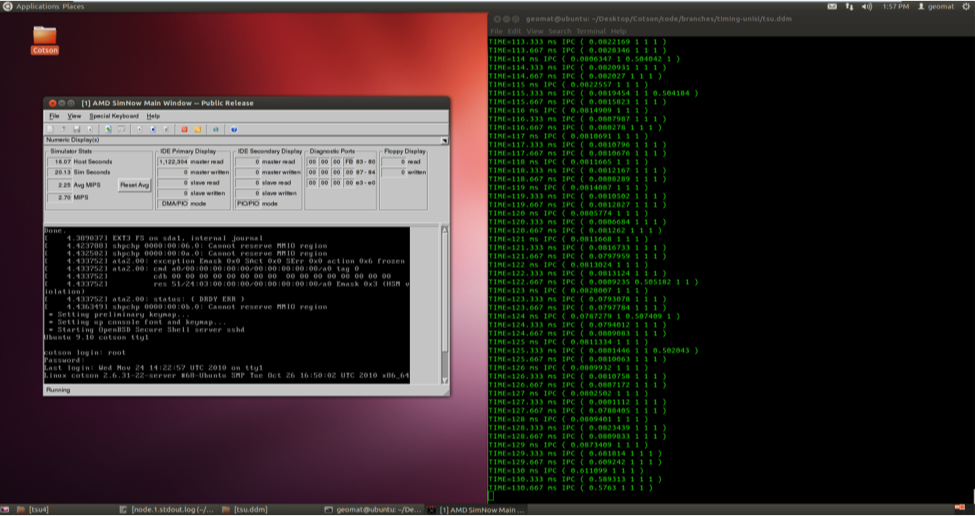
\includegraphics[width=6.4146in,height=3.3945in]{img50.png}
\par}

{\centering\selectlanguage{english}\sffamily\bfseries
\label{bkm:Ref388170875}Fig.
\stepcounter{Figure}{\theFigure} - Executing TSU++ on COTSon.
\par}

{\selectlanguage{english}
The output is stored in the \textit{node.1.stdout.log }file. It should
display a content similar to the following:}



\begin{center}
\begin{minipage}{6.3465in}
{\selectlanguage{english}
Worker 0: stack 0xa2f000 16384}

{\selectlanguage{english}
Worker 1: stack 0xa34000 16384}

{\selectlanguage{english}
Worker 2: stack 0xa39000 16384}

{\selectlanguage{english}
Worker 3: stack 0xa3e000 16384}

{\selectlanguage{english}
Program: Cholesky decomposition, Cores 4, AQ threshold: 2, Matrix Size:
2048, BlockSize: 32}

{\selectlanguage{english}
Deallocate worker frame at 0xa2f000}

{\selectlanguage{english}
Deallocate worker frame at 0xa34000}

{\selectlanguage{english}
Deallocate worker frame at 0xa39000}

{\selectlanguage{english}
Deallocate worker frame at 0xa3e000}

{\selectlanguage{english}
All workers done, goodbye}

{\selectlanguage{english}
Speedup: \ \ \ \ \ \ 3.480233}

{\selectlanguage{english}
Serial time: \ \ 24.089845}

{\selectlanguage{english}
Parallel time: 6.921906}
\end{minipage}
\end{center}

\bigskip


\bigskip


\bigskip


\bigskip


\bigskip


\bigskip


\bigskip


\bigskip

\subsection[Further references to more in{}-depths]{Further references
to more in-depths}
{\selectlanguage{english}
none.}

\section[Research Use Case from UD]{Research Use Case from UD}
{\selectlanguage{english}
{The
}\textit{{Delaware
Adaptive Run-Time
System}}{ (DARTS)
is a software implementation of the
}\textit{{Codelet
Model}}{ proposed
by Zuckerman et al. [4]. It was written with two main objectives in
mind: (1) to be a faithful implementation of the Codelet Model, and (2)
to be modular, so that further research to explore fine-grain
event-driven program execution models could be performed.}}

{\selectlanguage{english}
{DARTS relies on the
}\textit{{hwloc
library}}{ [1] to
map the topology of the underlying hardware to the Codelet abstract
machine model required to specify how many synchronization units
(similar to DF-Threads{\textquotesingle} thread scheduling units) and
compute units (or cores) there should be, and how they should be
physically grouped. It also relies on the lock-free data structures
provided by Intel Threading Building Blocks [3] if they are present on
the system for efficient work queuing.}}

{\selectlanguage{english}
{Further details
about the implementation of DARTS on the generic X86 architecture can
be found in the Euro-Par publication [2]. A detailed explanation of the
port of DARTS to the TERAFLUX simulation infrastructure, including a
discussion of the necessary trade-offs.}}

\subsection[Goal of the experiment or example]{Goal of the experiment or
example}
{\selectlanguage{english}
This example demonstrates how to build and run examples that come with
the port of DARTS on COTSon simulation infrastructure. In the following
it will be demonstrated how to first build DARTS, then run the
experiments. The focus will be on the \textit{merge sort} example,
however all the other experiments can be built using a similar
methodology.}

\subsection[Location of the involved files]{Location of the involved
files}
{\selectlanguage{english}
The archive for DARTS-TSUF can be found at: \ }

\begin{flushleft}
\tablehead{}
\begin{supertabular}{|m{6.29346in}|}
\hline
\selectlanguage{english}
\texttt{\$COTSON\_ROOT/branches/ud-darts/darts-tsuf}\\\hline
\end{supertabular}
\end{flushleft}
{\selectlanguage{english}
The directory containing scripts to run the recursive Fibonacci sequence
computation, Matrix Multiplication, and Merge Sort examples is located
at: }

\begin{flushleft}
\tablehead{}
\begin{supertabular}{|m{6.29346in}|}
\hline
\selectlanguage{english}
\texttt{\$COTSON\_ROOT/branches/ud-darts/scripts}\\\hline
\end{supertabular}
\end{flushleft}
\subsection[Detailed instructions to start]{Detailed instructions to
start}
{\selectlanguage{english}
The Merge Sort example can be run by typing the following commands. In
the following, it is considered that the COTSon repository is located
in the path pointed by the variable \textbf{\$COTSON}. The directory
where to install and run the experiments is pointed by the variable
\textbf{\$PATH\_TO\_EXPERIMENTS }(note that the two variables can be
defined by the user).}

\begin{itemize}
\item {\selectlanguage{english}
Building DARTS-TSUF. \ After having checked the
COTSon{\textquotesingle}s files out, do:}
\end{itemize}
\begin{flushleft}
\tablehead{}
\begin{supertabular}{|m{6.29346in}|}
\hline
{\selectlanguage{english}\ttfamily \$ cd \$PATH\_TO\_EXPERIMENTS/}

{\selectlanguage{english}\ttfamily \$ mkdir
\$PATH\_TO\_EXPERIMENTS/darts-build}

{\selectlanguage{english}\ttfamily \$ cd
\$PATH\_TO\_EXPERIMENTS/darts-build}

{\selectlanguage{english} \texttt{\$ cmake
\$COTSON\_ROOT/branches/ud-darts/darts-tsuf}}

\selectlanguage{english}\ttfamily \$ make\\\hline
\end{supertabular}
\end{flushleft}
\begin{itemize}
\item {\selectlanguage{english}
Running the DARTS-TSUF merge-sort example. First, copy the scripts from
the script folder as follows:}
\end{itemize}
\begin{flushleft}
\tablehead{}
\begin{supertabular}{|m{6.29346in}|}
\hline
{\selectlanguage{english}\ttfamily \$ mkdir
\$PATH\_TO\_EXPERIMENTS/scripts}

{\selectlanguage{english}\ttfamily \$ cd
\$PATH\_TO\_EXPERIMENTS/scripts}

\selectlanguage{english} \texttt{\$ cp
\$COTSON\_ROOT/branches/ud-darts/scripts/* .}\\\hline
\end{supertabular}
\end{flushleft}
{\selectlanguage{english}
Configure the \textit{config.lua}\texttt{ }script so that it points to
the right \textit{tflux\_tsu.so}\texttt{ }library, as well as the right
script to run (in this example, \textit{msort.sh}). Then edit
\textit{msort.sh}{\textquotesingle}s variables:}

\begin{flushleft}
\tablehead{}
\begin{supertabular}{|m{6.29346in}|}
\hline
{\selectlanguage{english}\ttfamily \$ export
OUTPUT\_PATH=\$PATH\_TO\_EXPERIMENTS}

{\selectlanguage{english}\ttfamily \$ export
DARTS\_PATH=\$PATH\_TO\_EXPERIMENTS/darts-build}

{\selectlanguage{english} \texttt{\$ export
COTSON\_PATH=\$COTSON\_ROOT/trunk/bin}}

\selectlanguage{english}\ttfamily \$ ./launch.sh\\\hline
\end{supertabular}
\end{flushleft}
\subsection[Expected output]{Expected output}
{\selectlanguage{english}
The output is stored in the \textit{results.txt} file. It should display
a content similar to the following:}

\begin{flushleft}
\tablehead{}
\begin{supertabular}{|m{6.29346in}|}
\hline
{\selectlanguage{english}\ttfamily DF owm 0x7ffff7674000 10000000}

{\selectlanguage{english}\ttfamily Creating 1 workers for 1 cores}

{\selectlanguage{english}\ttfamily Starting workers}

{\selectlanguage{english}\ttfamily Starting master node 1 nodes 1
workers 1}

{\selectlanguage{english}\ttfamily mergesort(500)}

{\selectlanguage{english}\ttfamily Done}

{\selectlanguage{english}\ttfamily Time:2.39678e+08 ns}

{\selectlanguage{english}\ttfamily Deallocate OWM at 0x7ffff7674000}

{\selectlanguage{english}\ttfamily All workers done, goodbye}

{\selectlanguage{english}
\texttt{=========================================================}}

{\selectlanguage{english}\ttfamily ==================== \ \ \ DF STATS
\ \ ======================}

{\selectlanguage{english}\ttfamily df time: \ 240736779 ns (240.737 ms)}

\selectlanguage{english}\ttfamily core \ 0: \ 23360631 insts 240736779
xc \ \ \ \ \ \ \ \ 0 ic, 240736779 cycles\\\hline
\end{supertabular}
\end{flushleft}
{\selectlanguage{english}
The number of elements to be sorted is displayed (the example tries to
merge 500 random numbers). If the simulation went through, the
{\textquotedblleft}Done{\textquotedblright} message is displayed,
followed (on the next line) by the amount of in-simulation nanoseconds
it took to run the experiment.}

\subsection[Further references to more in{}-depths]{Further references
to more in-depths}
{\selectlanguage{english}
none. }

\section[Research Use Case from UNIMAN]{Research Use Case from UNIMAN}
{\selectlanguage{english}
Our main goal is the design and implementation of Transactional memory
(TM) system in the COTSon simulator. We have developed TM system that
supports lazy and eager version management and conflict detection
mechanism. The TM models have been extended and a scalable TM system
has been developed. The scalable system is a purely lazy implementation
but the commit process takes advantage of a hierarchical organization
of cores into nodes. The committed changes are broadcasted within the
node but outside the node the invalidations are sent only to the nodes
that were actually sharing the committed data. In order to implement
the scalable TM system we have used directory based cache coherence
protocol as a starting point for our baseline version.}

{\selectlanguage{english}
In the following subsections, we will be explaining in detail of how to
run our TM models in the COTSon simulator along with the directory
based protocols on which our scalable TM version is based on.}

\subsection[Goal of the experiment or example]{Goal of the experiment or
example}
{\selectlanguage{english}
The main goal of the experiment is to show how to run different
benchmarks on the TM system developed in COTSon. We will show how to
run applications on scalable directory based simulator as well as the
TM system implemented on top of the directory infrastructure. We will
also be giving detailed description of running dataflow benchmarks with
transactions running on the simulator. We will be showing how the TM
model works along with the TSU to run dataflow plus transactional
memory benchmarks.}

\subsection[Location of the involved files]{Location of the involved
files}
{\selectlanguage{english}
The complete TM infrastructure is present in the following two
locations.}

\begin{flushleft}
\tablehead{}
\begin{supertabular}{|m{6.29346in}|}
\hline
\selectlanguage{english}\ttfamily
\$COTSONHOME/branches/tm-uniman\\\hline
\end{supertabular}
\end{flushleft}
{\selectlanguage{english}
And}

\begin{flushleft}
\tablehead{}
\begin{supertabular}{|m{6.29346in}|}
\hline
\selectlanguage{english}\ttfamily
\$COTSONHOME/branches/tflux-test/tsuf\\\hline
\end{supertabular}
\end{flushleft}
{\selectlanguage{english}
First is the cache coherent NUMA architecture. The code for this
directory based coherent architecture is present in:}

\begin{flushleft}
\tablehead{}
\begin{supertabular}{|m{6.29346in}|}
\hline
\selectlanguage{english}
\texttt{\$COTSONHOME/branches/tm-uniman/trunk/src}\\\hline
\end{supertabular}
\end{flushleft}
{\selectlanguage{english}
The configuration files for the scalable system are present in:}

\begin{flushleft}
\tablehead{}
\begin{supertabular}{|m{6.29346in}|}
\hline
\selectlanguage{english}
\texttt{\$COTSONHOME/branches/tm-uniman/trunk/src/example/uniman/cc\_numa\_tracer}\\\hline
\end{supertabular}
\end{flushleft}
{\selectlanguage{english}
The code for the TM system developed at uniman is present in}

\begin{flushleft}
\tablehead{}
\begin{supertabular}{|m{6.29346in}|}
\hline
\selectlanguage{english}
\texttt{\$COTSONHOME/branches/tm-uniman/trunk/src}\\\hline
\end{supertabular}
\end{flushleft}
{\selectlanguage{english}
And the configuration files are in}

\begin{flushleft}
\tablehead{}
\begin{supertabular}{|m{6.29346in}|}
\hline
\selectlanguage{english}
\texttt{\$COTSONHOME/branches/tm-uniman/trunk/src/example/uniman/tm\_tracer}\\\hline
\end{supertabular}
\end{flushleft}
{\selectlanguage{english}
The code for the scalable TM system is present in}

{\selectlanguage{english}
\texttt{\$COTSONHOME/branches/tm-uniman/trunk/src}}

{\selectlanguage{english}
And the configuration files are in}

\begin{flushleft}
\tablehead{}
\begin{supertabular}{|m{6.29346in}|}
\hline
\selectlanguage{english}
\texttt{\$COTSONHOME/branches/tm-uniman/trunk/src/example/uniman/tm\_tracer\_scalable}\\\hline
\end{supertabular}
\end{flushleft}
{\selectlanguage{english}
Finally the configuration files to run TM system along with the TSU to
run dataflow plus transactional benchmarks are present in}

\begin{flushleft}
\tablehead{}
\begin{supertabular}{|m{6.29346in}|}
\hline
\selectlanguage{english}
\texttt{\$COTSONHOME/branches/tflux-test/tsuf/test}\\\hline
\end{supertabular}
\end{flushleft}
{\selectlanguage{english}
We will be looking at all these files and give example of running simple
benchmarks on all these configurations in order to help the user in
using our TM infrastructure for further experimentation.}

\subsection[Detailed instructions to start]{Detailed instructions to
start}
{\selectlanguage{english}
The first step is to check out the full COTSon repository (including
branches) and set \texttt{\$COTSONHOME}:}

\begin{flushleft}
\tablehead{}
\begin{supertabular}{|m{6.29346in}|}
\hline
{\selectlanguage{english} \texttt{\$ svn co
}\texttt{https://svn.code.sf.net/p/cotson/code cotson}}

\selectlanguage{english} \texttt{\$ export
COTSONHOME={\textless}installation\_dir{\textgreater}/cotson}\\\hline
\end{supertabular}
\end{flushleft}
{\selectlanguage{english}
Next the user has to compile the main trunk and also the
{\textquoteleft}branches/tm-uniman/trunk{\textquoteright}:}

\begin{flushleft}
\tablehead{}
\begin{supertabular}{|m{6.29346in}|}
\hline
{\selectlanguage{english} \texttt{\$ cd }\texttt{\$COTSONHOME/trunk}}

\selectlanguage{english}\ttfamily \$ ./configure --simnow\_dir
{\textless}path\_to\_simnow\_installation{\textgreater}\\\hline
\end{supertabular}
\end{flushleft}
{\selectlanguage{english}
if the configure terminate successfully than just type:}

\begin{flushleft}
\tablehead{}
\begin{supertabular}{|m{6.29346in}|}
\hline
\selectlanguage{english}\ttfamily \$ make\\\hline
\end{supertabular}
\end{flushleft}
{\selectlanguage{english}
Again for
{\textquotedblleft}branches/tm-uniman/trunk{\textquotedblright}:}

\begin{flushleft}
\tablehead{}
\begin{supertabular}{|m{6.29346in}|}
\hline
{\selectlanguage{english} \texttt{\$ cd
}\texttt{\$COTSONHOME/branches/tm-uniman/trunk}}

{\selectlanguage{english}\ttfamily \$ ./configure --simnow\_dir
{\textless}path\_to\_simnow\_installation{\textgreater}}

\selectlanguage{english}\ttfamily \$ make\\\hline
\end{supertabular}
\end{flushleft}
{\selectlanguage{english}
\textbf{Running benchmarks on Scalable ccNUMA architecture}}

{\selectlanguage{english}
In order to run scalable directory based \textit{ccNUMA} architecture we
need to configure the COTSon simulator:}

\begin{flushleft}
\tablehead{}
\begin{supertabular}{|m{6.29346in}|}
\hline
\selectlanguage{english} \texttt{\$ cd
\$COTSONHOME/branches/tm-uniman/trunk/src/examples/uniman/cc\_numa\_tracer}\\\hline
\end{supertabular}
\end{flushleft}
{\selectlanguage{english}
The main file that configures the system is \textit{cotson\_tracer.in}.
Fig. 35, shows the snapshot of that configuration file.}

{\centering 
\includegraphics[width=5.6091in,height=2.6244in]{img51.png}
\par}

{\centering\selectlanguage{english}\sffamily\bfseries
\label{bkm:Ref388170890}Fig.
\stepcounter{Figure}{\theFigure} -- Configuring ccNUMA architecture in
COTSon.
\par}

{\selectlanguage{english}
The configuration file sets up the number of nodes in the system
\textit{totalNumOfNodes} as well as total number of cores in each node.
It also sets up the directory structure and the protocol being used to
implement coherency.}

{\selectlanguage{english}
In the same directory there is the file \textit{run.sh}, which contains
paths of all the benchmarks that need to run on the simulator (in the
examples directory there are several benchmarks, in this case the
default is Micro-Benchmarks/microtest). In order to run benchmarks the
user just needs to type \textit{make}. The result containing all the
execution statistics is saved in the log file after the simulation
exits successfully, in the same directory.}

{\selectlanguage{english}
\textbf{Running benchmarks on TM architecture}}

{\selectlanguage{english}
Configuration files for TM architecture are reached by issuing:}

\begin{flushleft}
\tablehead{}
\begin{supertabular}{|m{6.29346in}|}
\hline
\selectlanguage{english} \texttt{\$ cd
\$COTSONHOME/branches/tm-uniman/trunk/src/examples/uniman/tm\_tracer}\\\hline
\end{supertabular}
\end{flushleft}
{\selectlanguage{english}
\textit{cotson\_tracer}.\textit{in} file configures the simulator to run
TM benchmarks. Fig. 36 shows the screenshot of that configuration
file.}

{\centering 
\includegraphics[width=6.2661in,height=2.7862in]{img52.png}
\par}

{\centering\selectlanguage{english}\sffamily\bfseries
\label{bkm:Ref388170901}Fig.
\stepcounter{Figure}{\theFigure} -- Configuring TM architecture in
COTSon.
\par}

{\selectlanguage{english}
As shown in the figure, the configuration file sets up the TM protocol.
It configures the network and the caches used in implementing TM
protocol. The caches are modified to contain extra information for
saving and committing transactional data.}

{\selectlanguage{english}
In the same directory there is the file \textit{run.sh}, which contains
paths of all the benchmarks that need to run on the simulator (in this
case, the path to \textit{vacation} binary). In order to run benchmark
the user just needs to type \textit{make}. The result containing all
the statistics of the execution is saved in the log file after the
simulation exits successfully, in the same directory.}

{\selectlanguage{english}
\textbf{Running benchmarks on Scalable TM System }}

{\selectlanguage{english}
Scalable TM system builds on top of directory based protocols. The
configuration files to implement the scalable TM system are reached by
issuing:}

\begin{flushleft}
\tablehead{}
\begin{supertabular}{|m{6.29346in}|}
\hline
\selectlanguage{english} \texttt{\$ cd
\$COTSONHOME/branches/tm-uniman/trunk/src/examples/uniman/tm\_tracer\_scalable}\\\hline
\end{supertabular}
\end{flushleft}
{\selectlanguage{english}
\textit{cotson\_tracer.in} file configures the simulator to run TM
benchmarks. Fig. 37 shows the screenshot of the configuration file.}

{\selectlanguage{english}
As shown in the figure, the configuration file sets up the scalable TM
protocol. It configures the network, the caches and the directories
used in implementing TM protocol. The caches and the directories are
modified to contain extra information for saving and committing
transactional data and implementing the TM protocol. Directories are
configured to implement the TM protocol rather than conventional
coherence protocol.}

{\selectlanguage{english}
To run the benchmark (\textit{Micro-Benchmarks/microtest} in this case)
the user has to do a \textit{make}. The file \textit{run.sh} contains
paths of all the benchmarks and the log file contains all the stats of
the execution.}

{\centering 
\includegraphics[width=5.4709in,height=2.7898in]{img53.png}
\par}

{\centering\selectlanguage{english}\sffamily\bfseries
\label{bkm:Ref388170914}Fig.
\stepcounter{Figure}{\theFigure} -- Configuring TM architecture in
COTSon.
\par}

{\selectlanguage{english}
\textbf{Running dataflow plus TM benchmark in COTSon using TSU and TM
hardware}}

{\selectlanguage{english}
This section explains how to set up the simulator so that it has both
the TSU and TM hardware working together to run applications that have
dataflow and transaction properties.}

{\selectlanguage{english}
In order to run dataflow and transaction benchmarks, the COTSon
simulator needs to implement the TSU hardware as well as TM hardware so
that both aspects of the applications can be handled in hardware for
greater efficiency.}

{\selectlanguage{english}
The configuration files to set up TM mechanism along with TSU hardware
are reached by issuing:}

\begin{flushleft}
\tablehead{}
\begin{supertabular}{|m{6.29346in}|}
\hline
{\selectlanguage{english} \texttt{\$ cd
\$COTSONHOME/branches/tflux-test/tsuf}}

{\selectlanguage{english}\ttfamily \$ make}

{\selectlanguage{english} \texttt{\$ cd
\$COTSONHOME/branches/tflux-test/tsuf/test}}

\selectlanguage{english}\ttfamily \$ make run\_htm\_single \ \ \ (or
make run\_htm\_multi)\\\hline
\end{supertabular}
\end{flushleft}
{\selectlanguage{english}
There are two configuration files \textit{tsu\_tm\_single.lua} and
\textit{tsu\_tm\_multi.lua}\textbf{\textit{ }}to run single node and
multi node simulation respectively. The user has to do a \textit{make}
run\_htm\_single or make run\_htm\_multi. The snapshot of the make file
in shown in Fig. 38.}

{\selectlanguage{english}
As shown in the figure, the makefile sets up TM running on single and
multi-node with the TSU hardware. The \textit{tsu\_tm\_single.lua} and
\textit{tsu\_tm\_multi.lua}\textbf{\textit{ }}\textit{files }configure
the network, the caches and the directories used in implementing TM
protocol.}

{\selectlanguage{english}
To run the benchmark the user has to do a \textit{make}. HTMTESTS
variable in the makefile contains the list of the benchmarks to run.
The log file contains all the stats after the execution exits
successfully.}

{\centering 
\includegraphics[width=5.8965in,height=2.4984in]{img54.png}
\par}

{\centering\selectlanguage{english}\sffamily\bfseries
\label{bkm:Ref388170927}Fig.
\stepcounter{Figure}{\theFigure} -- Makefile to setup TM and TSU
hardware for single and multimode simulation.
\par}

\subsection[Expected output]{Expected output}
{\selectlanguage{english}
This section explains some of the output files that are generated when
the execution successfully exits. We will also be showing some screen
shots to show the execution in progress and the output that should be
expected when running the benchmarks.}

{\selectlanguage{english}
\textbf{Running benchmark on Scalable ccNUMA architecture}}

{\selectlanguage{english}
Fig. 39 shows the devices when running ccNUMA COTSon simulation. The
\textit{cotson\_tracer.in} sets up the number of cores in the system as
shown in Fig. 40. In this example the number of cores is 4, which is
reflected in Fig. 39. The log file is generated when the execution
successfully exits. Fig. 41shows the snapshot of the log file, which is
generated when the matrix multiplication example finished execution.
The log file shows the cache stats of the simulation running with 4
cores.}

{\centering 
\includegraphics[width=2.6874in,height=1.8244in]{img55.png}
\par}

{\centering\selectlanguage{english}\sffamily\bfseries
\label{bkm:Ref388170940}Fig.
\stepcounter{Figure}{\theFigure} -- Device window while running COTSon
simulation
\par}

{\centering 
\includegraphics[width=6.1764in,height=1.1665in]{img56.png}
\par}

{\centering\selectlanguage{english}\sffamily\bfseries
\label{bkm:Ref388170955}Fig.
\stepcounter{Figure}{\theFigure} -- cotson\_tracer.in configuration
file setting up the number of cores in the simulated machine
\par}

{\centering 
\includegraphics[width=3.0402in,height=2.3965in]{img57.png}
\par}

{\centering\selectlanguage{english}\sffamily\bfseries
\label{bkm:Ref388170970}Fig.
\stepcounter{Figure}{\theFigure} -- Log file showing icache statistics
for the cpu 0.
\par}

{\selectlanguage{english}
\textbf{Running benchmarks on TM architecture}}

{\selectlanguage{english}
Fig. 42 shows the COTSon simulation running \textit{vacation}
transactional memory benchmark. As you can see in the figure the number
of commits and aborts are printed in the console. }

{\centering 
\includegraphics[width=5.0382in,height=2.6638in]{img58.png}
\par}

{\centering\selectlanguage{english}\sffamily\bfseries
\label{bkm:Ref388170981}Fig.
\stepcounter{Figure}{\theFigure} -- COTSon graphical main window and
the console output.
\par}

{\selectlanguage{english}
The output of the benchmark is printed on the COTSon main graphical
window. Finally the simulation stats are written to the log file that
is created in the same folder where the configuration files are
present.}

{\selectlanguage{english}\bfseries
Running benchmarks on Scalable TM architecture}

{\selectlanguage{english}
Fig. 43 shows COTSon simulation running \textit{Genome} benchmark. The
figure shows how the scalable TM system is configured containing many
nodes, distributed memory structure and a shared L3 cache within each
node. }

{\centering 
\includegraphics[width=4.9618in,height=2.3728in]{img59.png}
\par}

{\centering\selectlanguage{english}\sffamily\bfseries
\label{bkm:Ref388170993}Fig.
\stepcounter{Figure}{\theFigure} -- Configuring the scalable TM
architecture in COTSon.
\par}

{\selectlanguage{english}
This configuration is setup in the \textit{cotson\_tracer.lua}
configuration file. The structure of the system can be changed by
making modifications in the lua file. The user can increase or decrease
the number of cores within a node. The levels of cache hierarchy, the
directory and network structure can also be configured. The log file is
created when the simulation exits successfully.}

{\centering 
\includegraphics[width=4.9736in,height=2.4126in]{img60.png}
\par}

{\centering\selectlanguage{english}\sffamily\bfseries
\label{bkm:Ref388171011}Fig.
\stepcounter{Figure}{\theFigure} -- COTSon simulation setting up and
running TM and TSU hardware.
\par}

{\selectlanguage{english}
\textbf{Running dataflow plus TM benchmark in COTSon using TSU and TM
hardware}}

{\selectlanguage{english}
The final experiment we will show in this report is how to run TM
hardware along with the TSU hardware for benchmarks that have
transactions and dataflow properties. Fig. 44 shows the COTSon
simulation configuring and then running a simple micro benchmark using
the TM and TSU hardware. The dataflow instructions are handled by the
TSU hardware and the transactional memory instructions are handled by
the TM hardware. The log file is created at the end, with all the
simulation statistics.}

\subsection[Further references to more in{}-depths]{Further references
to more in-depths}
{\selectlanguage{english}
none.}

\section[Research Use Case from UNISI]{Research Use Case from UNISI}
\label{bkm:Ref388221943}{\selectlanguage{english}
One of the main building blocks of the TERAFLUX project is the
implementation of the Thread Scheduling Unit (TSU) model, running in
the COTSon simulation platform. As result of the research activity,
several versions of the TSU model has been implemented and made
available to the other partners. The two most stable versions at the
current moment are the TSUF and the TSU4. Both of them allow the
execution of dataflow benchmark kernels (such as the \textit{recursive
Fibonacci}, and \textit{Matrix Multiplication}) both on a single node
simulated system, and a multi-node simulated system. The purpose of the
TSU model is the scheduling of dataflow threads (namely DF-Threads)
among the available cores, as expected from the hardware counterpart.}

\subsection[Goal of the experiment or example]{Goal of the experiment or
example}
{\selectlanguage{english}
The main goal of the experiment is to show how to run a dataflow
benchmark application using the TSU model developed within the COTSon
simulator. To this end, the following subsections describe how to run a
simple test using the TSU4 model (for the TSUF implementation, refers
to the chapter 9, sections from 9.1 to 9.5). The experiment allows the
user to understand how the scheduling unit model has been integrated in
the simulation platform, and which information it provides to the
user.}

\subsection[Location of the involved files]{Location of the involved
files}
{\selectlanguage{english}
The scheduling unit model is distributed in a dedicated directory
contained in the \textit{branches} folder:}

\begin{flushleft}
\tablehead{}
\begin{supertabular}{|m{6.34626in}|}
\hline
\selectlanguage{english}
\texttt{\$COTSONROOT/branches/timing-unisi/tsu4}\\\hline
\end{supertabular}
\end{flushleft}
\subsection[Detailed instructions to start]{Detailed instructions to
start}
{\selectlanguage{english}
As an example, detailed instructions to run the \textit{recursive
Fibonacci} benchmark kernel on the TSU4 model of the thread scheduling
unit will be provided. This benchmark is used to stress the thread
scheduling unit since it is able to generate a huge number of
DF-Threads even for a small size of the input. In order to run the
example, move on the correct folder:}

\begin{flushleft}
\tablehead{}
\begin{supertabular}{|m{6.34626in}|}
\hline
\selectlanguage{english} \texttt{\$ cd
\$COTSONROOT/branches/timing-unisi/tsu4}\\\hline
\end{supertabular}
\end{flushleft}
{\selectlanguage{english}
Open the \textit{Makefile} file with a text editor and check that the
first line is correctly pointing the source folder in the trunk COTSon
folder. Then, in the same file set the variable \textit{TESTS} to
\textit{fib}, in order to run the selected benchmark:}

\begin{flushleft}
\tablehead{}
\begin{supertabular}{|m{6.34626in}|}
\hline
\selectlanguage{english}\ttfamily \$ vim Makefile\\\hline
{\selectlanguage{english}\ttfamily ROOT=../../../trunk/src}

{\selectlanguage{english}\ttfamily DATE=\$(shell date +\%s)}

{\selectlanguage{english}\ttfamily PWD=\$(shell pwd)}

{\selectlanguage{english}\ttfamily MCAST=\$(shell expr 1 + \$(DATE) \%
250)}

{\selectlanguage{english}\ttfamily DEBUG=1}

{\selectlanguage{english}\ttfamily TESTS = fib}

~

{\selectlanguage{english}\ttfamily all: tsu\_monitor.o tsu\_manager.o
tflux\_tsu.so tsumon \$(TESTS)}

\selectlanguage{english}\ttfamily ...\\\hline
\end{supertabular}
\end{flushleft}
{\selectlanguage{english}
Open the \textit{run\_script.sh} file with a text editor. In the opened
file set the variable \textit{TESTS} to \textit{fib}, in order to run
the selected benchmark. In order to properly set the configuration of
the simulated system (i.e., size of the input of the benchmark, number
of cores, etc.), the following variables must be checked:
\textit{NUM\_NODE} defines the number of nodes composing the system,
\textit{CORES} defines the number of cores in each node, \textit{SZ}
and \textit{MT\_SIZE} define the input size for the used benchmark
(\textit{SZ} refers to the \textit{Fibonacci} kernel, while
\textit{MT\_SIZE} refers to the \textit{Matrix Multiplication} kernel).
In this example the \textit{Fibonacci} kernel with 14 as the input size
is run. \textit{SH\_MEM} variable defines the name of the object in the
host system used to implement the shared memory across the nodes.
Finally, \textit{OUTPUT} variable point to the folder where the
simulation output will be recorded (set also \textit{TSU\_STATS},
\textit{SCRIPT}, and \textit{REPORT\_DIR} variables).}

\begin{flushleft}
\tablehead{}
\begin{supertabular}{|m{6.34626in}|}
\hline
\selectlanguage{english}\ttfamily \$ vim run\_script.sh\\\hline
{\selectlanguage{english}\ttfamily !/bin/bash}

~

{\selectlanguage{english}\ttfamily \# number of nodes}

{\selectlanguage{english}\ttfamily NUM\_NODE=1}

{\selectlanguage{english}\ttfamily \# benchmarks}

{\selectlanguage{english}\ttfamily
TESTS={\textquotedbl}fib{\textquotedbl}}

{\selectlanguage{english}\ttfamily \# number of cores per node}

{\selectlanguage{english}\ttfamily CORES=4}

{\selectlanguage{english}\ttfamily TTCORES=\$((\$CORES*\$NUM\_NODE))}

{\selectlanguage{english}\ttfamily \#for fibonacci}

{\selectlanguage{english}\ttfamily SZ=14}

{\selectlanguage{english}\ttfamily \#for matrix multiply}

{\selectlanguage{english} \texttt{MT\_SIZE=512}\texttt{ \# matrix size}}

{\selectlanguage{english}\ttfamily \#shared memory name (unique for each
simulation)}

{\selectlanguage{english}\ttfamily
SH\_MEM={\textquotedbl}DTHREADSharedMemory{\textquotedbl}}

~

{\selectlanguage{english}\ttfamily if [[ \$SH\_MEM ]]; then}

{\selectlanguage{english}\ttfamily \ \ \ \ export
DTHREAD\_OBJ=\$SH\_MEM{\textquotedbl}1{\textquotedbl}}

{\selectlanguage{english}\ttfamily \ \ \ \ export
DTHREAD\_READY\_OBJ=\$SH\_MEM{\textquotedbl}2{\textquotedbl}}

{\selectlanguage{english}\ttfamily \ \ \ \ export
DTSU\_SYNC\_OBJ=\$SH\_MEM{\textquotedbl}3{\textquotedbl}}

{\selectlanguage{english}\ttfamily fi}

~

{\selectlanguage{english}\ttfamily BIN\_BENCH\_DIR=\$PWD}

~

{\selectlanguage{english} \texttt{if [ -z \$OUTPUT ] ; then
}\texttt{OUTPUT=./S-LOG}\texttt{ ; fi}}

~

{\selectlanguage{english}\ttfamily
SCRIPT={\textquotedbl}\$OUTPUT/script{\textquotedbl}}

{\selectlanguage{english}\ttfamily
TSU\_STATS={\textquotedbl}\$OUTPUT/stats{\textquotedbl}}

{\selectlanguage{english}\ttfamily
FILE\_LAST\_LOG={\textquotedbl}file\_last{\textquotedbl}}

{\selectlanguage{english}\ttfamily
REPORT\_DIR={\textquotedbl}\$OUTPUT/report{\textquotedbl}}

\selectlanguage{english}\ttfamily ...\\\hline
\end{supertabular}
\end{flushleft}
{\selectlanguage{english}
The Lua configuration file is set to run a timing simulation
(\textit{sampler} object is set to \textit{simple}) of the target
system:}

\begin{flushleft}
\tablehead{}
\begin{supertabular}{|m{6.34626in}|}
\hline
\selectlanguage{english}\ttfamily \$ vim tsu.lua\\\hline
{\selectlanguage{english}\ttfamily
abaeterno\_so={\textquotedbl}tflux\_tsu.so{\textquotedbl}}

{\selectlanguage{english}\ttfamily
wd=os.getenv({\textquotedbl}PWD{\textquotedbl})}

~

{\selectlanguage{english}\ttfamily tmpdir=wd}

{\selectlanguage{english}\ttfamily
runid={\textquotedbl}tsu{\textquotedbl}}

{\selectlanguage{english}\ttfamily {}-{}- clean\_sandbox=false}

~

{\selectlanguage{english}\ttfamily options = \{}

{\selectlanguage{english}\ttfamily
\ \ \ \ \ \ \ \ {}-{}-max\_nanos={\textquotesingle}3G{\textquotesingle},}

{\selectlanguage{english}\ttfamily
\ \ \ \ \ \ \ \ exit\_trigger={\textquotesingle}terminate{\textquotesingle},}

{\selectlanguage{english}\ttfamily \ \ \ \ \ \ \ \ {}-{}-
sampler=\{type={\textquotedbl}no\_timing{\textquotedbl},
quantum={\textquotedbl}10M{\textquotedbl}\},}

{\selectlanguage{english}
\texttt{\ \ \ \ \ \ \ \ }\texttt{sampler=\{type={\textquotedbl}simple{\textquotedbl},
quantum={\textquotedbl}10M{\textquotedbl}\},}}

{\selectlanguage{english}\ttfamily \ \ \ \ \ \ \ \ heartbeat=\{
type={\textquotedbl}file\_last{\textquotedbl},
logfile=runid..{\textquotedbl}.log{\textquotedbl} \},}

{\selectlanguage{english}\ttfamily \ \ \ \ \ \ \ \ custom\_asm=true,}

{\selectlanguage{english}\ttfamily
\ \ \ \ \ \ \ \ tsu\_ignore\_errors=true,}

{\selectlanguage{english}\ttfamily \ \ \ \ \ \ \ \ {}-{}-
tsu\_speculative\_threads=true,}

{\selectlanguage{english}\ttfamily \ \ \ \ \ \ \ \ {}-{}-
tsu\_statfile={\textquotedbl}/tmp/xx.dat{\textquotedbl},}

{\selectlanguage{english}\ttfamily \}}

~

{\selectlanguage{english}\ttfamily
one\_node\_script={\textquotedbl}run\_interactive{\textquotedbl}}

{\selectlanguage{english}\ttfamily {}-{}-
display=os.getenv({\textquotedbl}DISPLAY{\textquotedbl})}

{\selectlanguage{english}\ttfamily
copy\_files\_prefix=runid..{\textquotedbl}.{\textquotedbl}}

{\selectlanguage{english}\ttfamily {}-{}- clean\_sandbox=false}

~

{\selectlanguage{english}\ttfamily simnow.commands=function()}

{\selectlanguage{english}\ttfamily \ \ \ \ \ \ \ \ {}-{}-
use\_bsd({\textquotesingle}32p.bsd{\textquotesingle})}

{\selectlanguage{english}\ttfamily
\ \ \ \ \ \ \ \ use\_bsd({\textquotesingle}4p.bsd{\textquotesingle})}

{\selectlanguage{english}\ttfamily \ \ \ \ \ \ \ \ {}-{}-
use\_bsd(BSDS)}

{\selectlanguage{english}\ttfamily
\ \ \ \ \ \ \ \ use\_hdd({\textquotesingle}karmic64.img{\textquotesingle})}

{\selectlanguage{english}\ttfamily
\ \ \ \ \ \ \ \ {}-{}-use\_hdd({\textquotesingle}debian.img{\textquotesingle})}

{\selectlanguage{english}\ttfamily \ \ \ \ \ \ \ \ set\_journal()}

{\selectlanguage{english}\ttfamily
\ \ \ \ send\_keyboard({\textquotesingle}xget
{\textquotesingle}..SCRIPT..{\textquotesingle}
script{\textquotesingle})}

{\selectlanguage{english}\ttfamily
\ \ \ \ send\_keyboard({\textquotesingle}sh -x script {\textbar} tee
LOG 2{\textgreater}\&1{\textquotesingle})}

{\selectlanguage{english}\ttfamily end}

~

{\selectlanguage{english}\ttfamily function build()}

{\selectlanguage{english}\ttfamily \ \ \ \ \ \ \ \ i=0}

\selectlanguage{english}\ttfamily ...\\\hline
\end{supertabular}
\end{flushleft}

At this point is possible to launch the simulation. To this end, the
reader needs to open two console windows. In the first console (after
moving in the \textit{\$COTSON-ROOT/branches/timing-unisi/tsu4}) the
reader launches the external monitor (i.e., the object that is used to
manage the shared memory across the nodes)

\begin{flushleft}
\tablehead{}
\begin{supertabular}{|m{6.34626in}|}
\hline
\selectlanguage{english}\ttfamily \$ make run\_tsumon\\\hline
\end{supertabular}
\end{flushleft}
{\selectlanguage{english}
Once the monitor is running, the following output should be presented:}

\begin{flushleft}
\tablehead{}
\begin{supertabular}{|m{6.34626in}|}
\hline
{\selectlanguage{english}\ttfamily \$Booting TSU Monitor
...}

{\selectlanguage{english}\ttfamily \$Start TSU Monitor}

{\selectlanguage{english}\ttfamily \$TSU Monitor is
configured with 1 nodes}

{\selectlanguage{english}\ttfamily \$TSU Monitor is
initializing shared memory (DTHREADSharedMemory1) \$....}

{\selectlanguage{english}\ttfamily \$TSU Monitor is
initializing ready shared memory (DTHREADSharedMemory2) ....}

{\selectlanguage{english}\ttfamily \$TSU Monitor is
initializing sync shared memory (DTHREADSharedMemory3) ....}

{\selectlanguage{english}\ttfamily \$TSU message queue
m2n(DTHREADSharedMemory1mq\_mon2node0) for node(0) is initializing....}

{\selectlanguage{english}\ttfamily \$TSU message queue
n2m(DTHREADSharedMemory1mq\_node2mon0) for node(0) is initializing....}

\selectlanguage{english}\ttfamily \$Initialization for
shared memory finished!\\\hline
\end{supertabular}
\end{flushleft}
{\selectlanguage{english}
Finally, on the second console the user launches the benchmark execution
as follows:}

\begin{flushleft}
\tablehead{}
\begin{supertabular}{|m{6.34626in}|}
\hline
\selectlanguage{english}\ttfamily \$ make run\\\hline
\end{supertabular}
\end{flushleft}
\subsection[Expected output]{Expected output}
{\selectlanguage{english}
The following files are involved in the output process. The file
\textit{node.1.tsu.log }contains the statistics gathered by COTSon
during the simulation:}

\begin{flushleft}
\tablehead{}
\begin{tiny}
\begin{supertabular}{|m{6.34626in}|}
\hline
{\selectlanguage{english}\ttfamily Input values:}

{\selectlanguage{english}\ttfamily cpu0.bpred\_perfect
\ \ \ \ \ \ \ \ \ \ \ \ \ \ \ \ \ \ \ \ \ \ \ \ \ \ \ \ \ \ \ \ \ \ \ \ \ \ \ \ \ false}

{\selectlanguage{english}\ttfamily
cpu0.branch\_mispred\_penalty
\ \ \ \ \ \ \ \ \ \ \ \ \ \ \ \ \ \ \ \ \ \ \ \ \ \ \ \ \ \ \ \ 8}

{\selectlanguage{english}\ttfamily cpu0.commit\_cpi
\ \ \ \ \ \ \ \ \ \ \ \ \ \ \ \ \ \ \ \ \ \ \ \ \ \ \ \ \ \ \ \ \ \ \ \ \ \ \ \ \ \ \ \ 1.0}

{\selectlanguage{english}\ttfamily cpu0.dcache.fudge
\ \ \ \ \ \ \ \ \ \ \ \ \ \ \ \ \ \ \ \ \ \ \ \ \ \ \ \ \ \ \ \ \ \ \ \ \ \ \ \ \ \ 1.0}

{\selectlanguage{english}\ttfamily cpu0.icache.fudge
\ \ \ \ \ \ \ \ \ \ \ \ \ \ \ \ \ \ \ \ \ \ \ \ \ \ \ \ \ \ \ \ \ \ \ \ \ \ \ \ \ \ 1.0}

{\selectlanguage{english}\ttfamily cpu0.twolev.hlength
\ \ \ \ \ \ \ \ \ \ \ \ \ \ \ \ \ \ \ \ \ \ \ \ \ \ \ \ \ \ \ \ \ \ \ \ \ \ \ \ 14}

{\selectlanguage{english}\ttfamily cpu0.twolev.l1\_size
\ \ \ \ \ \ \ \ \ \ \ \ \ \ \ \ \ \ \ \ \ \ \ \ \ \ \ \ \ \ \ \ \ \ \ \ \ \ \ \ 1}

{\selectlanguage{english}\ttfamily cpu0.twolev.l2\_size
\ \ \ \ \ \ \ \ \ \ \ \ \ \ \ \ \ \ \ \ \ \ \ \ \ \ \ \ \ \ \ \ \ \ \ \ \ \ \ \ 16kB}

{\selectlanguage{english}\ttfamily cpu0.twolev.use\_xor
\ \ \ \ \ \ \ \ \ \ \ \ \ \ \ \ \ \ \ \ \ \ \ \ \ \ \ \ \ \ \ \ \ \ \ \ \ \ \ \ 1}

{\selectlanguage{english}\ttfamily cpu0.type
\ \ \ \ \ \ \ \ \ \ \ \ \ \ \ \ \ \ \ \ \ \ \ \ \ \ \ \ \ \ \ \ \ \ \ \ \ \ \ \ \ \ \ \ \ \ \ \ \ \ timer0}

{\selectlanguage{english}\ttfamily cpu1.bpred\_perfect
\ \ \ \ \ \ \ \ \ \ \ \ \ \ \ \ \ \ \ \ \ \ \ \ \ \ \ \ \ \ \ \ \ \ \ \ \ \ \ \ \ false}

{\selectlanguage{english}\ttfamily
cpu1.branch\_mispred\_penalty
\ \ \ \ \ \ \ \ \ \ \ \ \ \ \ \ \ \ \ \ \ \ \ \ \ \ \ \ \ \ \ \ 8}

{\selectlanguage{english}\ttfamily cpu1.commit\_cpi
\ \ \ \ \ \ \ \ \ \ \ \ \ \ \ \ \ \ \ \ \ \ \ \ \ \ \ \ \ \ \ \ \ \ \ \ \ \ \ \ \ \ \ \ 1.0}

{\selectlanguage{english}\ttfamily cpu1.dcache.fudge
\ \ \ \ \ \ \ \ \ \ \ \ \ \ \ \ \ \ \ \ \ \ \ \ \ \ \ \ \ \ \ \ \ \ \ \ \ \ \ \ \ \ 1.0}

{\selectlanguage{english}\ttfamily cpu1.icache.fudge
\ \ \ \ \ \ \ \ \ \ \ \ \ \ \ \ \ \ \ \ \ \ \ \ \ \ \ \ \ \ \ \ \ \ \ \ \ \ \ \ \ \ 1.0}

{\selectlanguage{english}\ttfamily cpu1.twolev.hlength
\ \ \ \ \ \ \ \ \ \ \ \ \ \ \ \ \ \ \ \ \ \ \ \ \ \ \ \ \ \ \ \ \ \ \ \ \ \ \ \ 14}

{\selectlanguage{english}\ttfamily cpu1.twolev.l1\_size
\ \ \ \ \ \ \ \ \ \ \ \ \ \ \ \ \ \ \ \ \ \ \ \ \ \ \ \ \ \ \ \ \ \ \ \ \ \ \ \ 1}

{\selectlanguage{english}\ttfamily cpu1.twolev.l2\_size
\ \ \ \ \ \ \ \ \ \ \ \ \ \ \ \ \ \ \ \ \ \ \ \ \ \ \ \ \ \ \ \ \ \ \ \ \ \ \ \ 16kB}

{\selectlanguage{english}\ttfamily ...}

{\selectlanguage{english}\ttfamily Output values:}

{\selectlanguage{english}\ttfamily cpu0.cycles
\ \ \ \ \ \ \ \ \ \ \ \ \ \ \ \ \ \ \ \ \ \ \ \ \ \ \ \ \ \ \ \ \ \ \ \ \ \ \ \ \ \ \ \ \ \ \ \ 149999985}

{\selectlanguage{english}\ttfamily cpu0.haltcount
\ \ \ \ \ \ \ \ \ \ \ \ \ \ \ \ \ \ \ \ \ \ \ \ \ \ \ \ \ \ \ \ \ \ \ \ \ \ \ \ \ \ \ \ \ 108195301}

{\selectlanguage{english}\ttfamily cpu0.hb\_ATC\_flush
\ \ \ \ \ \ \ \ \ \ \ \ \ \ \ \ \ \ \ \ \ \ \ \ \ \ \ \ \ \ \ \ \ \ \ \ \ \ \ \ \ \ 67}

{\selectlanguage{english}\ttfamily cpu0.hb\_CR3\_different
\ \ \ \ \ \ \ \ \ \ \ \ \ \ \ \ \ \ \ \ \ \ \ \ \ \ \ \ \ \ \ \ \ \ \ \ \ \ 36}

{\selectlanguage{english}\ttfamily cpu0.hb\_CR3\_equal
\ \ \ \ \ \ \ \ \ \ \ \ \ \ \ \ \ \ \ \ \ \ \ \ \ \ \ \ \ \ \ \ \ \ \ \ \ \ \ \ \ \ 31}

{\selectlanguage{english}\ttfamily cpu0.hb\_ev\_Exception
\ \ \ \ \ \ \ \ \ \ \ \ \ \ \ \ \ \ \ \ \ \ \ \ \ \ \ \ \ \ \ \ \ \ \ \ \ \ \ 692}

{\selectlanguage{english}\ttfamily cpu0.hb\_ev\_HW\_interrupt
\ \ \ \ \ \ \ \ \ \ \ \ \ \ \ \ \ \ \ \ \ \ \ \ \ \ \ \ \ \ \ \ \ \ \ \ 219}

{\selectlanguage{english}\ttfamily cpu0.hb\_ev\_SW\_interrupt
\ \ \ \ \ \ \ \ \ \ \ \ \ \ \ \ \ \ \ \ \ \ \ \ \ \ \ \ \ \ \ \ \ \ \ \ 0}

{\selectlanguage{english}\ttfamily cpu0.idlecount
\ \ \ \ \ \ \ \ \ \ \ \ \ \ \ \ \ \ \ \ \ \ \ \ \ \ \ \ \ \ \ \ \ \ \ \ \ \ \ \ \ \ \ \ \ 112802301}

{\selectlanguage{english}\ttfamily cpu0.instcount
\ \ \ \ \ \ \ \ \ \ \ \ \ \ \ \ \ \ \ \ \ \ \ \ \ \ \ \ \ \ \ \ \ \ \ \ \ \ \ \ \ \ \ \ \ 24655697}

{\selectlanguage{english}\ttfamily cpu0.invalid\_translation\_bytes
\ \ \ \ \ \ \ \ \ \ \ \ \ \ \ \ \ \ \ \ \ \ \ \ \ \ \ \ \ 1936557}

{\selectlanguage{english}\ttfamily cpu0.iocount
\ \ \ \ \ \ \ \ \ \ \ \ \ \ \ \ \ \ \ \ \ \ \ \ \ \ \ \ \ \ \ \ \ \ \ \ \ \ \ \ \ \ \ \ \ \ \ 4069258}

{\selectlanguage{english}\ttfamily cpu0.metadata\_bytes
\ \ \ \ \ \ \ \ \ \ \ \ \ \ \ \ \ \ \ \ \ \ \ \ \ \ \ \ \ \ \ \ \ \ \ \ \ \ \ \ 10468840}

{\selectlanguage{english}\ttfamily cpu0.other\_exceptions
\ \ \ \ \ \ \ \ \ \ \ \ \ \ \ \ \ \ \ \ \ \ \ \ \ \ \ \ \ \ \ \ \ \ \ \ \ \ 210511}

{\selectlanguage{english}\ttfamily cpu0.plain\_invalidations
\ \ \ \ \ \ \ \ \ \ \ \ \ \ \ \ \ \ \ \ \ \ \ \ \ \ \ \ \ \ \ \ \ \ \ 2988}

{\selectlanguage{english}\ttfamily cpu0.range\_invalidations
\ \ \ \ \ \ \ \ \ \ \ \ \ \ \ \ \ \ \ \ \ \ \ \ \ \ \ \ \ \ \ \ \ \ \ 32}

{\selectlanguage{english}\ttfamily cpu0.read\_mmios
\ \ \ \ \ \ \ \ \ \ \ \ \ \ \ \ \ \ \ \ \ \ \ \ \ \ \ \ \ \ \ \ \ \ \ \ \ \ \ \ \ \ \ \ 368}

{\selectlanguage{english}\ttfamily cpu0.read\_pios
\ \ \ \ \ \ \ \ \ \ \ \ \ \ \ \ \ \ \ \ \ \ \ \ \ \ \ \ \ \ \ \ \ \ \ \ \ \ \ \ \ \ \ \ \ 1062}

{\selectlanguage{english}\ttfamily cpu0.segv\_exceptions
\ \ \ \ \ \ \ \ \ \ \ \ \ \ \ \ \ \ \ \ \ \ \ \ \ \ \ \ \ \ \ \ \ \ \ \ \ \ \ 0}

{\selectlanguage{english}\ttfamily cpu0.timer.cycles
\ \ \ \ \ \ \ \ \ \ \ \ \ \ \ \ \ \ \ \ \ \ \ \ \ \ \ \ \ \ \ \ \ \ \ \ \ \ \ \ \ \ 37823009}

{\selectlanguage{english}\ttfamily cpu0.timer.instructions
\ \ \ \ \ \ \ \ \ \ \ \ \ \ \ \ \ \ \ \ \ \ \ \ \ \ \ \ \ \ \ \ \ \ \ \ 24147071}

{\selectlanguage{english}\ttfamily cpu0.timer.twolev.lookup
\ \ \ \ \ \ \ \ \ \ \ \ \ \ \ \ \ \ \ \ \ \ \ \ \ \ \ \ \ \ \ \ \ \ \ 2048709}

{\selectlanguage{english}\ttfamily cpu0.timer.twolev.misses
\ \ \ \ \ \ \ \ \ \ \ \ \ \ \ \ \ \ \ \ \ \ \ \ \ \ \ \ \ \ \ \ \ \ \ 83286}

{\selectlanguage{english}\ttfamily cpu0.timer.twolev.reset
\ \ \ \ \ \ \ \ \ \ \ \ \ \ \ \ \ \ \ \ \ \ \ \ \ \ \ \ \ \ \ \ \ \ \ \ 0}

{\selectlanguage{english}\ttfamily cpu0.timer.twolev.update
\ \ \ \ \ \ \ \ \ \ \ \ \ \ \ \ \ \ \ \ \ \ \ \ \ \ \ \ \ \ \ \ \ \ \ 2048709}

{\selectlanguage{english}\ttfamily cpu0.trace\_cache\_size
\ \ \ \ \ \ \ \ \ \ \ \ \ \ \ \ \ \ \ \ \ \ \ \ \ \ \ \ \ \ \ \ \ \ \ \ \ \ 0}

{\selectlanguage{english}\ttfamily cpu0.valid\_translation\_bytes
\ \ \ \ \ \ \ \ \ \ \ \ \ \ \ \ \ \ \ \ \ \ \ \ \ \ \ \ \ \ \ 90649248}

{\selectlanguage{english}\ttfamily cpu0.write\_mmios
\ \ \ \ \ \ \ \ \ \ \ \ \ \ \ \ \ \ \ \ \ \ \ \ \ \ \ \ \ \ \ \ \ \ \ \ \ \ \ \ \ \ \ 564}

{\selectlanguage{english}\ttfamily cpu0.write\_pios
\ \ \ \ \ \ \ \ \ \ \ \ \ \ \ \ \ \ \ \ \ \ \ \ \ \ \ \ \ \ \ \ \ \ \ \ \ \ \ \ \ \ \ \ 4169}

{\selectlanguage{english}\ttfamily cpu1.cycles
\ \ \ \ \ \ \ \ \ \ \ \ \ \ \ \ \ \ \ \ \ \ \ \ \ \ \ \ \ \ \ \ \ \ \ \ \ \ \ \ \ \ \ \ \ \ \ \ 149999985}

{\selectlanguage{english}\ttfamily cpu1.haltcount
\ \ \ \ \ \ \ \ \ \ \ \ \ \ \ \ \ \ \ \ \ \ \ \ \ \ \ \ \ \ \ \ \ \ \ \ \ \ \ \ \ \ \ \ \ 121463351}

{\selectlanguage{english}\ttfamily cpu1.hb\_ATC\_flush
\ \ \ \ \ \ \ \ \ \ \ \ \ \ \ \ \ \ \ \ \ \ \ \ \ \ \ \ \ \ \ \ \ \ \ \ \ \ \ \ \ \ 24}

{\selectlanguage{english}\ttfamily cpu1.hb\_CR3\_different
\ \ \ \ \ \ \ \ \ \ \ \ \ \ \ \ \ \ \ \ \ \ \ \ \ \ \ \ \ \ \ \ \ \ \ \ \ \ 1}

{\selectlanguage{english}\ttfamily cpu1.hb\_CR3\_equal
\ \ \ \ \ \ \ \ \ \ \ \ \ \ \ \ \ \ \ \ \ \ \ \ \ \ \ \ \ \ \ \ \ \ \ \ \ \ \ \ \ \ 23}

{\selectlanguage{english}\ttfamily cpu1.hb\_ev\_Exception
\ \ \ \ \ \ \ \ \ \ \ \ \ \ \ \ \ \ \ \ \ \ \ \ \ \ \ \ \ \ \ \ \ \ \ \ \ \ \ 504}

{\selectlanguage{english}\ttfamily cpu1.hb\_ev\_HW\_interrupt
\ \ \ \ \ \ \ \ \ \ \ \ \ \ \ \ \ \ \ \ \ \ \ \ \ \ \ \ \ \ \ \ \ \ \ \ 30}

{\selectlanguage{english}\ttfamily cpu1.hb\_ev\_SW\_interrupt
\ \ \ \ \ \ \ \ \ \ \ \ \ \ \ \ \ \ \ \ \ \ \ \ \ \ \ \ \ \ \ \ \ \ \ \ 0}

{\selectlanguage{english}\ttfamily cpu1.idlecount
\ \ \ \ \ \ \ \ \ \ \ \ \ \ \ \ \ \ \ \ \ \ \ \ \ \ \ \ \ \ \ \ \ \ \ \ \ \ \ \ \ \ \ \ \ 121840334}

\selectlanguage{english}\ttfamily ...\\\hline
\end{supertabular}
\end{tiny}
\end{flushleft}
{\selectlanguage{english}
The file \textit{terminal\_fib\_0\_4 }(enter in the subfolder
\textit{S-LOG} -- see the \textit{Makefile} configuration in the
previous subsection) contains the output generated by the benchmark and
the simulator during the simulation:}

\begin{flushleft}
\tablehead{}
\begin{tiny}
\begin{supertabular}{|m{6.34626in}|}
\hline
{\selectlanguage{english}\ttfamily Loading module
abaeterno.so.}

{\selectlanguage{english}\ttfamily Using image path:
{\textquotedbl}/home/scionti/Tools/cotson-release/trunk/data{\textquotedbl}}

{\selectlanguage{english}\ttfamily Known Device: Deerhound
RevB QuadCore Socket L1}

{\selectlanguage{english}\ttfamily Known Device: Intel(R)
Pro/1000 MT/PT Desktop Network Adapter}

{\selectlanguage{english}\ttfamily Known Device: USB
JumpDrive}

{\selectlanguage{english}\ttfamily Known Device: AMD-8111
I/O Hub}

{\selectlanguage{english}\ttfamily Known Device: AMD-8131
PCI-X Controller}

{\selectlanguage{english}\ttfamily Known Device: AMD-8132
PCI-X Controller}

{\selectlanguage{english}\ttfamily Known Device: AMD-8151
AGP Tunnel}

{\selectlanguage{english}\ttfamily Known Device: Debugger}

{\selectlanguage{english}\ttfamily ...}

~

{\selectlanguage{english}\ttfamily 1 exec{\textgreater}
open /home/scionti/Tools/cotson-release/trunk/data/4p.bsd}

{\selectlanguage{english}\ttfamily Opening
{\textquotedbl}/home/scionti/Tools/cotson-release/trunk/data/4p.bsd{\textquotedbl}}

{\selectlanguage{english}\ttfamily created device Machine}

{\selectlanguage{english}\ttfamily Instructions per
Microsecond: 3000}

{\selectlanguage{english}\ttfamily CPU Model Name: Opteron}

{\selectlanguage{english}\ttfamily System Bus Frequency:
100}

{\selectlanguage{english}\ttfamily CPU Clock Mul: 4}

{\selectlanguage{english}\ttfamily Turbo\_Port61: 0}

{\selectlanguage{english}\ttfamily Turbo\_Vsync: 0}

{\selectlanguage{english}\ttfamily Guard Memory Required:
TRUE}

{\selectlanguage{english}\ttfamily CPU Manages Cycles:
TRUE}

{\selectlanguage{english}\ttfamily Disk Block Cache Size:
64K}

{\selectlanguage{english}\ttfamily Disk Block Cache Depth:
5}

{\selectlanguage{english}\ttfamily Disk Block Cache Bits:
12}

{\selectlanguage{english}\ttfamily info: creating device
\#0 {\textquotedbl}AMD 8th Generation Integrated
Northbridge{\textquotedbl}}

{\selectlanguage{english}\ttfamily info: creating device
\#1 {\textquotedbl}Dimm Bank{\textquotedbl}}

{\selectlanguage{english}\ttfamily info: creating device
\#2 {\textquotedbl}AMD-8111 I/O Hub{\textquotedbl}}

{\selectlanguage{english}\ttfamily ATA: Image
[/home/scionti/Tools/cotson-release/trunk/data/karmic64.img] does not
have an ID field.}

{\selectlanguage{english}\ttfamily info: creating device
\#3 {\textquotedbl}Memory Device{\textquotedbl}}

{\selectlanguage{english}\ttfamily info: creating device
\#4 {\textquotedbl}Winbond W83627HF SIO{\textquotedbl}}

{\selectlanguage{english}\ttfamily ...}

{\selectlanguage{english}\ttfamily BSD Load completed!}

~

{\selectlanguage{english}\ttfamily 1 exec{\textgreater}
ide:0.image master
/home/scionti/Tools/cotson-release/trunk/data/karmic64.img}

{\selectlanguage{english}\ttfamily ATA: Image
[/home/scionti/Tools/cotson-release/trunk/data/karmic64.img] does not
have an ID field.}

{\selectlanguage{english}\ttfamily MASTER drive Image file
is now /home/scionti/Tools/cotson-release/trunk/data/karmic64.img}

~

{\selectlanguage{english}\ttfamily 1 exec{\textgreater}
ide:0.journal master on}

{\selectlanguage{english}\ttfamily Journaling was already
enabled}

~

{\selectlanguage{english}\ttfamily 1 exec{\textgreater}
keyboard.key 2D AD}

~

{\selectlanguage{english}\ttfamily 1 exec{\textgreater}
keyboard.key 22 A2}

~

{\selectlanguage{english}\ttfamily 1 exec{\textgreater}
keyboard.key 12 92}

~

{\selectlanguage{english}\ttfamily 1 exec{\textgreater}
keyboard.key 14 94}

~

{\selectlanguage{english}\ttfamily 1 exec{\textgreater}
keyboard.key 39 B9}

~

{\selectlanguage{english}\ttfamily 1 exec{\textgreater}
keyboard.key 34 B4}

~

{\selectlanguage{english}\ttfamily 1 exec{\textgreater}
keyboard.key 35 B5}

{\selectlanguage{english}\ttfamily ...}

{\selectlanguage{english}\ttfamily 1 exec{\textgreater} go}

{\selectlanguage{english}\ttfamily TIME=3.33333 ms IPC (
0.993879 0.707539 1 1 )}

{\selectlanguage{english}\ttfamily TIME=6.66667 ms IPC (
0.991326 0.98112 1 1 )}

{\selectlanguage{english}\ttfamily TIME=10 ms IPC ( 1 1 1 1
)}

{\selectlanguage{english}\ttfamily TIME=13.3333 ms IPC (
0.958046 0.8369 1 0.814146 )}

{\selectlanguage{english}\ttfamily TIME=16.6667 ms IPC (
0.99788 1 1 0.99697 )}

{\selectlanguage{english}\ttfamily TIME=20 ms IPC (
0.968307 0.966541 1 0.995992 )}

{\selectlanguage{english}\ttfamily TIME=23.3333 ms IPC (
0.774968 0.774076 1 0.982427 )}

{\selectlanguage{english}\ttfamily TIME=26.6667 ms IPC (
0.995373 1 1 0.965398 )}

{\selectlanguage{english}\ttfamily TIME=30 ms IPC ( 1 1 1 1
)}

{\selectlanguage{english}\ttfamily TIME=33.3333 ms IPC (
0.998995 0.999206 1 1 )}

{\selectlanguage{english}\ttfamily TIME=36.6667 ms IPC ( 1
1 1 0.99992 )}

{\selectlanguage{english}\ttfamily TIME=40 ms IPC ( 1 1 1 1
)}

{\selectlanguage{english}\ttfamily TIME=43.3333 ms IPC (
0.99907 0.999325 1 1 )}

{\selectlanguage{english}\ttfamily TIME=46.6667 ms IPC ( 1
1 1 0.999914 )}

{\selectlanguage{english}\ttfamily TIME=50 ms IPC ( 1 1 1 1
)}

{\selectlanguage{english}\ttfamily TIME=53.3333 ms IPC (
0.999072 0.999391 1 1 )}

{\selectlanguage{english}\ttfamily TIME=56.6667 ms IPC ( 1
1 1 0.99992 )}

{\selectlanguage{english}\ttfamily TIME=60 ms IPC ( 1 1 1 1
)}

{\selectlanguage{english}\ttfamily TIME=63.3333 ms IPC (
0.998833 0.999323 1 1 )}

{\selectlanguage{english}\ttfamily TIME=66.6667 ms IPC ( 1
1 1 1 )}

{\selectlanguage{english}\ttfamily TIME=70 ms IPC ( 1 1 1 1
)}

{\selectlanguage{english}\ttfamily TIME=73.3333 ms IPC (
0.998844 0.998883 1 1 )}

{\selectlanguage{english}\ttfamily TIME=76.6667 ms IPC ( 1
1 1 1 )}

{\selectlanguage{english}\ttfamily TIME=80 ms IPC ( 1 1 1 1
)}

{\selectlanguage{english}\ttfamily TIME=83.3333 ms IPC (
0.998409 0.999379 1 1 )}

{\selectlanguage{english}\ttfamily TIME=86.6667 ms IPC ( 1
1 1 1 )}

{\selectlanguage{english}\ttfamily TIME=90 ms IPC ( 1 1 1 1
)}

{\selectlanguage{english}\ttfamily TIME=93.3333 ms IPC (
0.998437 0.999356 1 1 )}

{\selectlanguage{english}\ttfamily TIME=96.6667 ms IPC ( 1
1 1 1 )}

{\selectlanguage{english}\ttfamily TIME=100 ms IPC ( 1 1 1
1 )}

{\selectlanguage{english}\ttfamily TIME=103.333 ms IPC (
0.998433 0.999404 1 1 )}

{\selectlanguage{english}\ttfamily TIME=106.667 ms IPC ( 1
1 1 1 )}

{\selectlanguage{english}\ttfamily TIME=110 ms IPC ( 1 1 1
1 )}

\selectlanguage{english}\ttfamily ...\\\hline
\end{supertabular}
\end{tiny}
\end{flushleft}

\bigskip

\subsection[Further references to more in{}-depths]{Further references
to more in-depths}
{\selectlanguage{english}
See paper [6] [18].}

\section[Appendix A {}-- Lua lexical
conventions]{\selectlanguage{english} Appendix A -- Lua lexical
conventions}
{\selectlanguage{english}
\textit{Names}~(also called~\textit{identifiers}) in Lua can be any
string of letters, digits, and underscores, not beginning with a digit.
This coincides with the definition of names in most languages. (The
definition of letter depends on the current locale: any character
considered alphabetic by the current locale can be used in an
identifier.) Identifiers are used to name variables and table fields.
{The
following~}\textit{{keywords}}{~are
reserved and cannot be used as names:}}

\begin{flushleft}
\tablehead{}
\begin{supertabular}{|m{1.1191599in}|m{1.1941599in}|m{1.1941599in}|m{1.1941599in}|m{1.2018598in}|}
\hline
\centering \selectlanguage{english}\bfseries and &
\centering \selectlanguage{english}\bfseries break &
\centering \selectlanguage{english}\bfseries do &
\centering \selectlanguage{english}\bfseries else &
\centering\arraybslash \selectlanguage{english}\bfseries elseif\\\hline
\centering \selectlanguage{english}\bfseries end &
\centering \selectlanguage{english}\bfseries false &
\centering \selectlanguage{english}\bfseries for &
\centering \selectlanguage{english}\bfseries function &
\centering\arraybslash \selectlanguage{english}\bfseries if\\\hline
\centering \selectlanguage{english}\bfseries in &
\centering \selectlanguage{english}\bfseries local &
\centering \selectlanguage{english}\bfseries nil &
\centering \selectlanguage{english}\bfseries not &
\centering\arraybslash \selectlanguage{english}\bfseries or\\\hline
\centering \selectlanguage{english}\bfseries repeat &
\centering \selectlanguage{english}\bfseries return &
\centering \selectlanguage{english}\bfseries then &
\centering \selectlanguage{english}\bfseries true &
\centering\arraybslash \selectlanguage{english}\bfseries until\\\hline
\centering \selectlanguage{english}\bfseries while &
~
 &
~
 &
~
 &
~
\\\hline
\end{supertabular}
\end{flushleft}

\bigskip

{\selectlanguage{english}
Lua is a case-sensitive language:~and~is a reserved word,
but~And~and~AND~are two different, valid names. As a convention, names
starting with an underscore followed by uppercase letters (such
as~VERSION) are reserved for internal global variables used by Lua. The
following strings denote other tokens:}

\begin{flushleft}
\tablehead{}
\begin{supertabular}{|m{1.1191599in}|m{1.1941599in}|m{1.1941599in}|m{1.1941599in}|m{1.2115599in}|}
\hline
\centering \selectlanguage{english}\bfseries + &
\centering \selectlanguage{english}\bfseries {}- &
\centering \selectlanguage{english}\bfseries * &
\centering \selectlanguage{english}\bfseries / &
\centering\arraybslash \selectlanguage{english}\bfseries \%\\\hline
\centering \selectlanguage{english}\bfseries \^{} &
\centering \selectlanguage{english}\bfseries \# &
\centering \selectlanguage{english}\bfseries == &
\centering \selectlanguage{english}\bfseries \~{}= &
\centering\arraybslash \selectlanguage{english}\bfseries
{\textless}=\\\hline
\centering \selectlanguage{english}\bfseries {\textgreater}= &
\centering \selectlanguage{english}\bfseries {\textless} &
\centering \selectlanguage{english}\bfseries {\textgreater} &
\centering \selectlanguage{english}\bfseries = &
\centering\arraybslash \selectlanguage{english}\bfseries (\\\hline
\centering \selectlanguage{english}\bfseries ) &
\centering \selectlanguage{english}\bfseries \{ &
\centering \selectlanguage{english}\bfseries \} &
\centering \selectlanguage{english}\bfseries [ &
\centering\arraybslash \selectlanguage{english}\bfseries ]\\\hline
\centering \selectlanguage{english}\bfseries ; &
\centering \selectlanguage{english}\bfseries : &
\centering \selectlanguage{english}\bfseries , &
\centering \selectlanguage{english}\bfseries . &
\centering\arraybslash \selectlanguage{english}\bfseries ..\\\hline
\centering \selectlanguage{english}\bfseries {\dots} &
~
 &
~
 &
~
 &
~
\\\hline
\end{supertabular}
\end{flushleft}
{\selectlanguage{english}
\textit{Literal strings}~can be delimited by matching single or double
quotes, and can contain the following C-like escape sequences:
{\textquotesingle}{\textbackslash}a{\textquotesingle} (bell),
{\textquotesingle}{\textbackslash}b{\textquotesingle} (backspace),
{\textquotesingle}{\textbackslash}f{\textquotesingle} (form feed),
{\textquotesingle}{\textbackslash}n{\textquotesingle} (newline),
{\textquotesingle}{\textbackslash}r{\textquotesingle} (carriage
return), {\textquotesingle}{\textbackslash}t{\textquotesingle}
(horizontal tab), {\textquotesingle}{\textbackslash}v{\textquotesingle}
(vertical tab),
{\textquotesingle}{\textbackslash}{\textbackslash}{\textquotesingle}
(backslash),
{\textquotesingle}{\textbackslash}{\textquotedbl}{\textquotesingle}
(quotation mark [double quote]), and
{\textquotesingle}{\textbackslash}{\textquotesingle}{\textquotesingle}
(apostrophe [single quote]). Moreover, a backslash followed by a real
newline results in a newline in the string. A character in a string can
also be specified by its numerical value using the escape
sequence~{\textbackslash}\textit{ddd}, where~\textit{ddd}~is a sequence
of up to three decimal digits. (Note that if a numerical escape is to
be followed by a digit, it must be expressed using exactly three
digits.) Strings in Lua can contain any 8-bit value, including embedded
zeros, which can be specified as
{\textquotesingle}{\textbackslash}0{\textquotesingle}.}

{\selectlanguage{english}
Literal strings can also be defined using a long format enclosed
by~\textit{long brackets}. We define an~\textit{opening long bracket of
level~n}~as an opening square bracket followed by~\textit{n}~equal
signs followed by another opening square bracket. So, an opening long
bracket of level~0 is written as~[[, an opening long bracket of level~1
is written as[=[, and so on. A~\textit{closing long bracket}~is defined
similarly; for instance, a closing long bracket of level~4 is written
as~]====]. A long string starts with an opening long bracket of any
level and ends at the first closing long bracket of the same level.
Literals in this bracketed form can run for several lines, do not
interpret any escape sequences, and ignore long brackets of any other
level. They can contain anything except a closing bracket of the proper
level.}

{\selectlanguage{english}
For convenience, when the opening long bracket is immediately followed
by a newline, the newline is not included in the string. As an example,
in a system using ASCII (in which {\textquotesingle}a{\textquotesingle}
is coded as~97, newline is coded as~10, and
{\textquotesingle}1{\textquotesingle} is coded as~49), the five literal
strings below denote the same string:}

\begin{flushleft}
\tablehead{}
\begin{supertabular}{|m{6.29346in}|}
\hline
{\selectlanguage{english}\ttfamily a =
{\textquotesingle}alo{\textbackslash}n123{\textquotedbl}{\textquotesingle}}

{\selectlanguage{english}\ttfamily a =
{\textquotedbl}alo{\textbackslash}n123{\textbackslash}{\textquotedbl}{\textquotedbl}}

{\selectlanguage{english}\ttfamily a =
{\textquotesingle}{\textbackslash}97lo{\textbackslash}10{\textbackslash}04923{\textquotedbl}{\textquotesingle}}

{\selectlanguage{english}\ttfamily a =
[[alo}

{\selectlanguage{english}\ttfamily
123{\textquotedbl}]]}

{\selectlanguage{english}\ttfamily a =
[==[}

{\selectlanguage{english}\ttfamily alo}

\selectlanguage{english}\ttfamily
123{\textquotedbl}]==]\\\hline
\end{supertabular}
\end{flushleft}
{\selectlanguage{english}\ttfamily
\foreignlanguage{english}{\textrm{{A~}}}\foreignlanguage{english}{\textrm{\textit{{numerical
constant}}}}\foreignlanguage{english}{\textrm{{~can
be written with an optional decimal part and an optional decimal
exponent. Lua also accepts integer hexadecimal constants, by prefixing
them with~0x. Examples of valid numerical constants are:}}}}

\begin{flushleft}
\tablehead{}
\begin{supertabular}{|m{6.29346in}|}
\hline
\selectlanguage{english}\ttfamily 3
\ \ 3.0 \ \ 3.1416 \ \ 314.16e-2 \ \ 0.31416E1 \ \ 0xff
\ \ 0x56\\\hline
\end{supertabular}
\end{flushleft}
{\selectlanguage{english}
{A}\textstyleappleconvertedspace{{~}}\textstyleEmphasis{{comment}}\textstyleappleconvertedspace{{~}}{starts
with a double hyphen
(}\textstyleHTMLCode{\textrm{{{}-{}-}}}{)
anywhere outside a string. If the text immediately
after}\textstyleappleconvertedspace{{~}}\textstyleHTMLCode{\textrm{{{}-{}-}}}\textstyleappleconvertedspace{{~}}{is
not an opening long bracket, the comment is
a}\textstyleappleconvertedspace{{~}}\textstyleEmphasis{{short
comment}}{, which runs until the end of the line.
Otherwise, it is a}\textstyleEmphasis{{long
comment}}{, which runs until the corresponding closing
long bracket. Long comments are frequently used to disable code
temporarily.}}


\bigskip

\section[Appendix B {}-- Lua language features]{\selectlanguage{english}
Appendix B -- Lua language features}
{\selectlanguage{english}
Lua is commonly described as a
{\textquotedblleft}multi-paradigm{\textquotedblright} language,
providing a small set of general features that can be extended to fit
different problem types, rather than providing a more complex and rigid
specification to match a single paradigm. Lua, for instance, does not
contain explicit support for
\href{http://en.wikipedia.org/wiki/Inheritance_(object-oriented_programming)}{inheritance},
but allows it to be implemented with
\href{http://en.wikipedia.org/wiki/Metatable}{metatables}. Similarly,
Lua allows programmers to implement
\href{http://en.wikipedia.org/wiki/Namespaces}{namespaces},
\href{http://en.wikipedia.org/wiki/Class_(computer_science)}{classes},
and other related features using its single table implementation;
\href{http://en.wikipedia.org/wiki/First-class_function}{first-class
functions} allow the employment of many techniques from
\href{http://en.wikipedia.org/wiki/Functional_programming}{functional
programming}; and full lexical
\href{http://en.wikipedia.org/wiki/Scope_(programming)}{scoping} allows
fine-grained
\href{http://en.wikipedia.org/wiki/Information_hiding}{information
hiding} to enforce the
\href{http://en.wikipedia.org/wiki/Principle_of_least_privilege}{principle
of least privilege}. In general, Lua strives to provide flexible
meta-features that can be extended as needed, rather than supply a
feature-set specific to one programming paradigm. As a result, the base
language is
\href{http://en.wikipedia.org/wiki/Lightweight_programming_language}{light}
-- the full reference
\href{http://en.wikipedia.org/wiki/Interpreter_(computing)}{interpreter}
is only about 180~\href{http://en.wikipedia.org/wiki/Kilobyte}{kB}
compiled -- and easily adaptable to a broad range of applications. Lua
is a \href{http://en.wikipedia.org/wiki/Dynamically_typed}{dynamically
typed} language intended for use as an
\href{http://en.wikipedia.org/wiki/Scripting_language}{extension} or
\href{http://en.wikipedia.org/wiki/Scripting_language}{scripting
language}, and is compact enough to fit on a variety of host platforms.
It supports only a small number of atomic data structures such as
\href{http://en.wikipedia.org/wiki/Boolean_data_type}{boolean} values,
\href{http://en.wikipedia.org/wiki/Number}{numbers} (double-precision
\href{http://en.wikipedia.org/wiki/Floating_point}{floating point} by
default), and
\href{http://en.wikipedia.org/wiki/String_(computer_science)}{strings}.
Typical data structures such as
\href{http://en.wikipedia.org/wiki/Array_data_structure}{arrays},
\href{http://en.wikipedia.org/wiki/Set_(computer_science)}{sets},
\href{http://en.wikipedia.org/wiki/List_(computing)}{lists}, and
\href{http://en.wikipedia.org/wiki/Record_(computer_science)}{records}
can be represented using Lua{\textquotesingle}s single native data
structure, the table, which is essentially a heterogeneous
\href{http://en.wikipedia.org/wiki/Associative_array}{associative
array}. Lua implements a small set of advanced features such as
\href{http://en.wikipedia.org/wiki/First-class_function}{first-class
functions},
\href{http://en.wikipedia.org/wiki/Garbage_collection_(computer_science)}{garbage
collection},
\href{http://en.wikipedia.org/wiki/Closure_(computer_science)}{closures},
proper \href{http://en.wikipedia.org/wiki/Tail_recursion}{tail calls},
\href{http://en.wikipedia.org/wiki/Type_conversion}{coercion}
(automatic conversion between string and number values at run time),
\href{http://en.wikipedia.org/wiki/Coroutine}{coroutines} (cooperative
multitasking) and
\href{http://en.wikipedia.org/wiki/Dynamic_loading}{dynamic module
loading}. By including only a minimum set of data types, Lua attempts
to strike a balance between power and size.}

{\selectlanguage{english}\bfseries
Loops}

{\selectlanguage{english}
Lua has four types of loops: the while loop, the repeat loop (similar to
a do while loop), the for loop, and the generic for loop.}

\begin{flushleft}
\tablehead{}
\begin{supertabular}{|m{6.21846in}|}
\hline
{\selectlanguage{english}\ttfamily
\foreignlanguage{english}{\textit{{{}-{}-condition
= true}}}\foreignlanguage{english}{{
}}}

{\selectlanguage{english}\ttfamily
\foreignlanguage{english}{\textbf{{while}}}\foreignlanguage{english}{{
condition
}}\foreignlanguage{english}{\textbf{{do}}}}

{\selectlanguage{english}\ttfamily
\foreignlanguage{english}{{\ \ }}\foreignlanguage{english}{\textit{{{}-{}-statements}}}}

{\selectlanguage{english}\ttfamily\bfseries
end}

~

~

{\selectlanguage{english}\ttfamily\bfseries
repeat}

{\selectlanguage{english}\ttfamily
\foreignlanguage{english}{{\ \ }}\foreignlanguage{english}{\textit{{{}-{}-statements}}}}

{\selectlanguage{english}\ttfamily
\foreignlanguage{english}{\textbf{{until}}}\foreignlanguage{english}{{
condition}}}

~

~

{\selectlanguage{english}\ttfamily
\foreignlanguage{english}{\textit{{{}-{}-delta
may be negative, allowing the for loop to count down or
up}}}\foreignlanguage{english}{{ }}}

{\selectlanguage{english}\ttfamily
\foreignlanguage{english}{\textbf{{for}}}\foreignlanguage{english}{{
i = first,last,delta
}}\foreignlanguage{english}{\textbf{{do}}}\foreignlanguage{english}{{
\ \ \ \ }}}

{\selectlanguage{english}\ttfamily
\foreignlanguage{english}{{\ \ }}\foreignlanguage{english}{\textit{{{}-{}-statements}}}}

{\selectlanguage{english}\ttfamily
\foreignlanguage{english}{{\ \ }}\foreignlanguage{english}{\textit{{{}-{}-example:
print(i)}}}}

\selectlanguage{english}\ttfamily\bfseries
end\\\hline
\end{supertabular}
\end{flushleft}
{\selectlanguage{english}
The generic \textit{for }loop, would iterate over the table\textit{ \_G}
using the standard iterator function pairs, until it returns
\textit{nil}:}

\begin{flushleft}
\tablehead{}
\begin{supertabular}{|m{6.21846in}|}
\hline
{\selectlanguage{english}\ttfamily
\textbf{\textit{{for}}}\textit{{
key, value
}}\textbf{\textit{{in}}}\textit{{
pairs(\_G) }}\textbf{\textit{{do}}}}

{\selectlanguage{english}\ttfamily\itshape
\ \ print(key, value)}

\selectlanguage{english}\ttfamily\bfseries\itshape
end\\\hline
\end{supertabular}
\end{flushleft}
{\selectlanguage{english}\bfseries
Functions}

{\selectlanguage{english}
Lua{\textquotesingle}s treatment of functions as first-class values is
shown in the following example, where the print
function{\textquotesingle}s behavior is modified:}

\begin{flushleft}
\tablehead{}
\begin{supertabular}{|m{6.21846in}|}
\hline
{\selectlanguage{english}\ttfamily\bfseries\itshape
do}

{\selectlanguage{english}\ttfamily
\foreignlanguage{english}{\textbf{\textit{{\ \ }}}}\foreignlanguage{english}{\textbf{\textit{{local}}}}\foreignlanguage{english}{\textit{{
oldprint = print}}}}

{\selectlanguage{english}\ttfamily\itshape
\ \ {}-{}- Store current print function as oldprint}

{\selectlanguage{english}\ttfamily
\foreignlanguage{english}{\textbf{\textit{{\ \ }}}}\foreignlanguage{english}{\textbf{\textit{{function}}}}\foreignlanguage{english}{\textit{{
print(s)}}}}

{\selectlanguage{english}\ttfamily\itshape
\ \ \ \ {}-{}-[[ Redefine print function, the usual print function can
still be used }

{\selectlanguage{english}\ttfamily\itshape
\ \ \ \ \ \ \ \ \ through oldprint. The new one has only one
argument.]]}

{\selectlanguage{english}\ttfamily\itshape
\ \ \ \ oldprint(s == {\textquotedbl}foo{\textquotedbl} and
{\textquotedbl}bar{\textquotedbl} or s)}

{\selectlanguage{english}\ttfamily
\foreignlanguage{english}{\textit{{\ \ }}}\foreignlanguage{english}{\textbf{\textit{{end}}}}}

\selectlanguage{english}\ttfamily\bfseries\itshape
end\\\hline
\end{supertabular}
\end{flushleft}
{\selectlanguage{english}
Any future calls to print will now be routed through the new function,
and because of Lua{\textquotesingle}s lexical scoping, the old print
function will only be accessible by the new, modified print.}

{\selectlanguage{english}\bfseries
Tables}

{\selectlanguage{english}
Tables are the most important data structure (and, by design, the only
built-in composite data type) in Lua, and are the foundation of all
user-created types. They are conceptually similar to associative arrays
in PHP, dictionaries in Python and Hashes in Ruby or Perl.}

{\selectlanguage{english}
A table is a collection of key and data pairs, where the data is
referenced by key; in other words, it{\textquotesingle}s a hashed
heterogeneous associative array. A key (index) can be any value but nil
and NaN. A numeric key of 1 is considered distinct from a string key of
{\textquotedbl}1{\textquotedbl}. Tables are created using the \{\}
constructor syntax:}

\begin{flushleft}
\tablehead{}
\begin{supertabular}{|m{6.21846in}|}
\hline
\selectlanguage{english}\ttfamily
\foreignlanguage{english}{\textbf{\textit{{a\_table
= \{\}
}}}}\foreignlanguage{english}{\textit{{{}-{}-
Creates a new, empty table}}}\\\hline
\end{supertabular}
\end{flushleft}
{\selectlanguage{english}
Tables are always passed by reference.}

{\selectlanguage{english}
\textbf{Record}}

{\selectlanguage{english}
A table is often used as structure (or record) by using strings as keys.
Because such use is very common, Lua features a special syntax for
accessing such fields. Example:}

\begin{flushleft}
\tablehead{}
\begin{supertabular}{|m{6.21846in}|}
\hline
{\selectlanguage{english}\ttfamily
\textbf{\textit{{point = \{ x = 10,
y = 20 }}}\textit{{\} \ \ {}-{}-
Create new table}}}

{\selectlanguage{english}\ttfamily
\textbf{\textit{{print(point[{\textquotedbl}x{\textquotedbl}])
\ \ \ \ \ \ \ \ \ \ \ }}}\textit{{{}-{}-
Prints 10}}}

\selectlanguage{english}\ttfamily
\foreignlanguage{english}{\textbf{\textit{{print(point.x)
\ \ \ \ \ \ \ \ \ \ \ \ \ \ }}}}\foreignlanguage{english}{\textit{{{}-{}-
Has exactly the same meaning as line above}}}\\\hline
\end{supertabular}
\end{flushleft}
{\selectlanguage{english}
\textbf{Array}}

{\selectlanguage{english}
By using a numerical key, the table resembles an array data type. Lua
arrays are 1-based: the first index is 1 rather than 0 as it is for
many other programming languages (though an explicit index of 0 is
allowed). A simple array of strings:}

\begin{flushleft}
\tablehead{}
\begin{supertabular}{|m{6.21846in}|}
\hline
{\selectlanguage{english}\ttfamily
\foreignlanguage{english}{\textbf{\textit{{array
= \{ {\textquotedbl}a{\textquotedbl}, {\textquotedbl}b{\textquotedbl},
{\textquotedbl}c{\textquotedbl}, {\textquotedbl}d{\textquotedbl} \}
}}}}\foreignlanguage{english}{\textit{{{}-{}-
Indices are assigned automatically.}}}}

{\selectlanguage{english}\ttfamily
\foreignlanguage{english}{\textbf{\textit{{print(array[2])
\ \ \ \ \ \ \ \ \ \ \ \ \ \ \ }}}}\foreignlanguage{english}{\textit{{{}-{}-
Prints {\textquotedbl}b{\textquotedbl}. Automatic indexing in
starts}}}\foreignlanguage{english}{\textbf{\textit{{
}}}}\foreignlanguage{english}{\textit{{at
1.}}}}

{\selectlanguage{english}\ttfamily
\foreignlanguage{english}{\textbf{\textit{{print(\#array)
\ \ \ \ \ \ \ \ \ \ \ \ \ \ \ \ \ }}}}\foreignlanguage{english}{\textit{{{}-{}-
Prints 4.}}}}

{\selectlanguage{english}\ttfamily
\foreignlanguage{english}{\textit{{\ \ \ \ \ \ \ \ \ \ \ \ \ \ \ \ \ \ \ \ \ \ \ \ \ \ \ \ \ \ \ }}}\foreignlanguage{english}{\textit{{{}-{}-
\# is length operator for tables and strings.}}}}

{\selectlanguage{english}\ttfamily
\foreignlanguage{english}{\textbf{\textit{{array[0]
= {\textquotedbl}z{\textquotedbl}
\ \ \ \ \ \ \ \ \ \ \ \ \ \ \ \ }}}}\foreignlanguage{english}{\textit{{{}-{}-
Zero is a legal index.}}}}

\selectlanguage{english}\ttfamily
\foreignlanguage{english}{\textbf{\textit{{print(\#array)
\ \ \ \ \ \ \ \ \ \ \ \ \ \ \ \ \ }}}}\foreignlanguage{english}{\textit{{{}-{}-
Still prints 4, as Lua arrays are 1-based.}}}\\\hline
\end{supertabular}
\end{flushleft}
\section[Appendix C {}-- DRT: A tool for native testing of T* based
programs]{\foreignlanguage{english}{Appendix C --
}DRT\foreignlanguage{english}{: A tool for native testing of T* based
programs}}
{\selectlanguage{english}
DARTS is not the only research effort for providing an efficient way to
execute application on large computing systems. Looking towards
building exascale systems (e.g., next generation supercomputers, large
data-centers, etc.), the OCR project (Open Community Run-time Framework
for Exascale Systems [5]) has been set up by Intel and other academic
and industrial partners. The main objective of the OCR project is the
implementation from the scratch (but reusing as much as possible
current design aspects of run-time systems) of a software level, which
is able to help meeting the requests of future exascale systems (i.e.,
high performance, low power consumption, use of different programming
models and languages, etc.). This piece of software should provide a
clear and common interface for both the upper side software modules,
and the hardware infrastructure. }

{\selectlanguage{english}
On the same direction, but with different goals in mind, the TERAFLUX
project proposed the Dataflow Run-Time -- DRT. In particular,
{with the aim of
facilitating the development and debugging of dataflow-oriented
applications using the T* ISA extension, within the TERAFLUX project, a
run-time library (DRT) has been devised. DRT is a piece of agile
software that helps in providing very efficient environment to run
programs with a dataflow execution model. It is organized as a library.
The library is intended to be linked with the application source code,
allowing the execution of the application directly on the host system.
More specifically, the run-time exposes the same interface of the
library used within the simulator to execute dataflow applications. The
library contains functions that wrap T* instructions. Similarly, the
DRT contains functions that reproduce the same functional behavior of
their T* equivalent [6]. The run-time Application Programming Interface
(API) has been designed to provide a two-way mechanism in which it
supports the development of an efficient compiler and on another side,
to provide for a good architectural support.}}

{\selectlanguage{english}
{In the proposed
approach, the DRT allows showing how easily can be to harness the
maximum capacity of the computing nodes in the TERAFLUX project using
the dataflow execution model. The main objective to provide this piece
of software is to show users that DRT can easily provide a very small
and powerful run-time, for executing different piece of codes that are
coded in different programming model, but how easily can be executed in
a dataflow style. }}

\subsection[Goal of the experiment ]{Goal of the experiment }
{\selectlanguage{english}
{DRT provides a simple
script file for the {\textquotedblleft}first time{\textquotedblright}
whole checking. Currently, some initial examples have been tested, from
simple (like the classical recursive Fibonacci sequence computation and
matrix multiplication). DRT contains some environment variables that
help the user to retrieve more information during the dataflow
application execution. Two of them are: DRT\_DEBUG and DRT\_FSIZE.
DRT\_DEBUG can be used to get more detailed information about the
current execution. DRT\_FSIZE is used to set the size of internal frame
(allocated memory) queue.}}

\subsection[Location of the involved files ]{Location of the involved
files }
{\selectlanguage{english}
The source code is uploaded for public access in following repository.
The repository is available at:}

\begin{flushleft}
\tablehead{}
\begin{supertabular}{|m{6.29346in}|}
\hline
\selectlanguage{english}
\texttt{http://sourceforge.net/projects/drt}\\\hline
\end{supertabular}
\end{flushleft}
\subsection[Detailed instructions to start \ ]{Detailed instructions to
start \foreignlanguage{english}{\ }}
{\selectlanguage{english}
{In this section, it
will be shown one sample example, and how to download and compile DRT
in a Linux-based system. }}

{\selectlanguage{english}
\textbf{{Step
1}}{: the user needs
to download the code from the repository. User can access the source
code from its Linux terminal executing the svn command. In the terminal
just type:}}

\begin{flushleft}
\tablehead{}
\begin{supertabular}{|m{6.29346in}|}
\hline
{\selectlanguage{english} \texttt{\$ svn checkout
svn://svn.code.sf.net/p/drt/code/ drt-code}}

\selectlanguage{english}\ttfamily \$ cd drt-code\\\hline
\end{supertabular}
\end{flushleft}
{\selectlanguage{english}
Pressing the enter key will start the download process (which can be
seen in the below snapshot).}

{\centering 
\includegraphics[width=4.3425in,height=1.8472in]{img61.png}
\par}

{\centering\selectlanguage{english}\sffamily\bfseries
Fig.
\stepcounter{Figure}{\theFigure} -- A DRT snapshot showing the download
process.
\par}

{\selectlanguage{english}
\textbf{{Step2:}}{
The user can notice the script file
}\textit{{tregression.sh}}{,
which can be used to check whether all the files are compiled
successfully or not. After executing this script, it will generate one
reference file and one output file for each example. The reader can
also control the debugging information level by exporting a new
variable called DRT\_DEBUG.}}

\begin{flushleft}
\tablehead{}
\begin{supertabular}{|m{6.29346in}|}
\hline
\selectlanguage{english}\ttfamily \$ ./tregression.sh\\\hline
\end{supertabular}
\end{flushleft}
{\centering 
\includegraphics[width=4.189in,height=3.6598in]{img62.png}
\par}

{\centering\selectlanguage{english}\sffamily\bfseries
Fig.
\stepcounter{Figure}{\theFigure} -- A DRT snapshot showing the result
of the tregression.sh script. During the compilation process, it is
produced in output an OK message (if no error is encountered)
\par}

\subsection[Expected output]{Expected output}
{\selectlanguage{english}
{The final step will be
to check a simple example: the recursive calculation of the Fibonacci
sequence. The program calculates the
15}{\textsuperscript{th}}{
Fibonacci number implementing the dataflow execution model.}}

{\centering 
\includegraphics[width=6.2626in,height=0.9717in]{img63.png}
\par}

{\centering\selectlanguage{english}\sffamily\bfseries
\label{bkm:Ref388171060}Fig.
\stepcounter{Figure}{\theFigure} -- DRT example execution: recursive
Fibonacci sequence with input set to 15 and debug level set to 0.
\par}

{\selectlanguage{english}
{As shown in
}{Fig.
47}{, the program
terminates with a correct result. As already mentioned, DRT can also
provide detailed information using the DRT\_DEBUG variable. The level
of verbosity can be increased using the increasing numbers (i.e., 0, 1,
2, 3, etc.). In the above example, the environmental variable has been
set to 0, by exporting it as
}\textit{{DRT\_DEBUG=0}}{.
It is worth noting that 0 corresponds to the default debug value. To
increase the verbosity level, just set the debug value to 1 (i.e.,
export the variable as DRT\_DEBUG=1).
}{Fig.
48}{ shows the result
of the program execution with the new debug level set.}}

{\centering 
\includegraphics[width=6.2646in,height=2.1465in]{img64.png}
\par}

{\centering\selectlanguage{english}\sffamily\bfseries
\label{bkm:Ref388171052}Fig.
\stepcounter{Figure}{\theFigure} -- DRT example execution: recursive
Fibonacci sequence with input set to 15 and debug level set to 1.
\par}

{\selectlanguage{english}
{So, by increasing this
verbosity level the user can retrieve more information about the
current execution.}}


\bigskip

%-------------------------------------------------------------
\clearpage
\section*{References}
\begin{flushleft}
\tablehead{}
\begin{supertabular}{m{0.39005986in}m{5.8705597in}}
\selectlanguage{english} [1] &
{\selectlanguage{english} Broquedis, F.; Clet-Ortega, J.; Moreaud, S.;
Furmento, N.; Goglin, B.; Mercier, G.; Thibault, S.; Namyst, R.,
\textit{hwloc: A Generic Framework for Managing Hardware Affinities in
HPC Applications}, Parallel, Distributed and Network-Based Processing
(PDP), 2010 18th Euromicro International Conference on , vol., no.,
pp.180,186, 17-19 Feb. 2010. }

\selectlanguage{english} URL:
\url{http://ieeexplore.ieee.org/stamp/stamp.jsp?tp=&arnumber=5452445&isnumber=5452403}\\
\selectlanguage{english} [2] &
{\selectlanguage{english} Joshua Suetterlein, St\'ephane Zuckerman, and
Guang R. Gao. 2013. An implementation of the codelet model. In
Proceedings of the 19th international conference on Parallel Processing
(Euro-Par{\textquotesingle}13), Felix Wolf, Bernd Mohr, and Dieter Mey
(Eds.). Springer-Verlag, Berlin, Heidelberg, 633-644.
DOI=10.1007/978-3-642-40047-6\_63.}

\selectlanguage{english} URL:
\url{http://dx.doi.org/10.1007/978-3-642-40047-6_63}\\
\selectlanguage{english} [3] &
{\selectlanguage{english} Thomas Willhalm and Nicolae Popovici. 2008.
Putting intel{\textregistered} threading building blocks to work. In
Proceedings of the 1st international workshop on Multicore software
engineering (IWMSE {\textquotesingle}08). ACM, New York, NY, USA, 3-4.
DOI=10.1145/1370082.1370085.}

\selectlanguage{english} URL:
\url{http://doi.acm.org/10.1145/1370082.1370085}\\
\selectlanguage{english} [4] &
\selectlanguage{english} St\'ephane Zuckerman, Joshua Suetterlein, Rob
Knauerhase, and Guang R. Gao. 2011. Using a
{\textquotedbl}codelet{\textquotedbl} program execution model for
exascale machines: position paper. In Proceedings of the 1st
International Workshop on Adaptive Self-Tuning Computing Systems for
the Exaflop Era (EXADAPT {\textquotesingle}11). ACM, New York, NY, USA,
64-69. DOI=10.1145/2000417.2000424. URL:
\url{http://doi.acm.org/10.1145/2000417.2000424}\\
\selectlanguage{english} [5] &
{\selectlanguage{english} {The
Open Community Runtime Framework for Exascale Systems. }

\selectlanguage{english} URL:
\url{https://01.org/open-community-runtime}}\\
\selectlanguage{english} [6] &
\selectlanguage{english}
Roberto Giorgi,
{\textquotedbl}TERAFLUX: Exploiting Dataflow Parallelism in
Teradevices{\textquotedbl}, ACM Computing Frontiers,
ISBN:978-1-4503-1215-8, Cagliari, Italy, May 2012, pp. 303-304, doi
10.1145/2212908.2212959,\\
\selectlanguage{english} [7] &
\selectlanguage{english} Aaron Landwehr, Stephane Zuckerman, Guang R.
Gao {\textquotedbl}Toward a Self-aware System for Exascale
Architectures{\textquotedbl}, In Proceedings of Euro-Par 2013: Parallel
Processing Workshops; the 1st Workshop on Runtime and Operating Systems
for the Many-core Era (ROME 2013), Aachen, Germany, August 2013.\\
\selectlanguage{english} [8] &
\selectlanguage{english} Joshua Suettlerlein, Stephane Zuckerman, Guang
R. Gao: {\textquotedbl}An Implementation of the Codelet
Model{\textquotedbl}. Euro-Par 2013, Aachen (Germany), August 2013,
doi: 10.1007/978-3-642-40047-6\_63.\\
\selectlanguage{english} [9] &
\selectlanguage{english} Bernhard Fechner, Arne Garbade, Sebastian Weis,
Theo Ungerer: {\textquotedbl}Fault Detection and Tolerance Mechanisms
for Future 1000 Core Systems{\textquotedbl}. HPCS 2013, Helsinki
(Finland), July 2013, doi: 10.1109/HPCSim.2013.6641467.\\
\selectlanguage{english} [10] &
\selectlanguage{english} George Matheou, Paraskevas Evripidou:
{\textquotedbl}Verilog-based simulation of hardware support for
Data-flow concurrency on Multicore systems{\textquotedbl}. SAMOS XIII
2013, Samos (Greece), July 2013, doi: 10.1109/SAMOS.2013.6621136.\\
\selectlanguage{english} [11] &
\selectlanguage{english} Javier Bueno, Xavier Martorell, Rosa M. Badia,
Eduard Ayguad\'e, Jes\'us Labarta: {\textquotedbl}Implementing OmpSs
support for regions of data in architectures with multiple address
spaces{\textquotedbl}. ISC {\textquotesingle}13: Proceedings of the
27th international ACM conference on International conference on
supercomputing, June 2013, doi: 10.1145/2464996.2465017.\\
\selectlanguage{english} [12] &
\selectlanguage{english} Fahimeh Yazdanpanah, Carlos Alvarz-Martinez,
Daniel Jimenez-Gonzalez, Yoav Etsion: {\textquotedbl}Hybrid
Dataflow/von-Neumann Architectures{\textquotedbl}. Parallel and
Distributed Systems, IEEE Transactions on (Volume:PP , Issue: 99),
April 2013, doi: 10.1109/TPDS.2013.125.\\
\selectlanguage{english} [13] &
\selectlanguage{english} A. Garbade, S. Weis, S. Schlingmann, B.
Fechner, T. Ungerer, {\textquotedbl}Impact of Message-Based Fault
Detectors on a Network on Chip,{\textquotedbl} in 21th International
Euromicro Conference on Parallel, Distributed and Network-based
Processing (PDP), Belfast, February 2013, doi: 10.1109/PDP.2013.76.\\
\selectlanguage{english} [14] &
\selectlanguage{english} Daniel Goodman, Behram Khan, Salman Khan, Mikel
Luj\'an, Ian Watson: {\textquotedbl}Software transactional memories for
Scala. J. Parallel Distrib. Comput{\textquotedbl}. (JPDC)
73(2):150-163, February 2013, doi: 10.1016/j.jpdc.2012.09.015.\\
\selectlanguage{english} [15] &
\selectlanguage{english} Nhat Minh L\^e, Antoniu Pop, Albert Cohen,
Francesco Zappa Nardelli: {\textquotedbl}Correct and efficient
work-stealing for weak memory models{\textquotedbl}. In Symp. on
Principles and Practice of Parallel Programming (PPoPP), Shenzhen,
China, February 2013, doi: 10.1145/2517327.2442524 and doi:
10.1145/2442516.2442524\\
\selectlanguage{english} [16] &
\selectlanguage{english} Boubacar Diouf, Can Hanta\c{s}, Albert Cohen,
\"Ozcan \"Ozturk, Jens Palsberg. {\textquotedbl}A decoupled local
memory allocator{\textquotedbl}. ACM Transactions on Architecture and
Code Optimization (TACO), selected for presentation at the HiPEAC 2013
Conf., January 2013, doi:10.1145/2400682.2400693\\
\selectlanguage{english} [17] &
\selectlanguage{english} Antoniu Pop and Albert Cohen.
{\textquotedbl}OpenStream: Expressiveness and Data-Flow compilation of
OpenMP streaming programs{\textquotedbl}. ACM Transactions on
Architecture and Code Optimization (TACO), selected for presentation at
the HiPEAC 2013 Conf., January 2013, doi: 10.1145/2400682.2400712\\
\selectlanguage{english} [18] &
\selectlanguage{english} R. Giorgi, R. M. Badia, F. Bodin, A. Cohen, P.
Evripidou, P. Faraboschi, B. Fechner, G. R. Gao, A. Garbade, R.
Gayatri, S. Girbal, D. Goodman, B. Khan, S. Kolia\"i, J. Landwehr, N.
Minh L, F. Li, M. Luj\`an, A. Mendelson, L. Morin, N. Navarro, T.
Patejko, A. Pop, P. Trancoso, T. Ungerer, I. Watson, S. Weis, S.
Zuckerman, M. Valero {\textquotedbl}TERAFLUX: Harnessing dataflow in
next generation teradevices{\textquotedbl}, Journal of Microprocessors
and Microsystems: Embedded Hardware Design (MICPRO), April 2014, doi:
doi.org/10.1016/j.micpro.2014.04.001\\
\end{supertabular}
\end{flushleft}

\bigskip
\end{document}
